  \documentclass[11pt]{article}
\usepackage{debulletin}
%\usepackage{deauthor}
\usepackage{times}
\usepackage{epsfig}
%\usepackage{subfigure}
\usepackage{wrapfig}
\usepackage{color}
\usepackage{boxedminipage}
\usepackage{graphicx}
\usepackage{url}
\usepackage{tabu}
\usepackage{multirow}
\usepackage{ulem}
\usepackage{layouts}
\usepackage[utf8]{inputenc}
\usepackage{paralist}
%\usepackage{thmtools} 
\usepackage{thm-restate}
\usepackage{dsfont}
%\usepackage{amsthm}
\usepackage{amsmath}
\usepackage{amssymb}
\usepackage{amsfonts}
\usepackage{hyperref}
\usepackage{enumitem}
\usepackage{xspace}
\usepackage{tikz}
\usepackage[T1]{fontenc}
\usepackage{beramono}
\usepackage{listings}
\usepackage{xcolor}
\usepackage{graphics}
\usepackage{pifont}
\usepackage{algorithmic}
\usepackage[sort&compress,numbers]{natbib}
\usepackage{microtype}
\usepackage{booktabs}
\usepackage{pgfplotstable}
\usepgfplotslibrary{groupplots}
\usepackage{bbm}
\usepackage{verbatim}
\usepackage{caption}
\usepackage{subcaption}
\usepackage{siunitx}
\usepackage[autostyle, english=american]{csquotes}
\usepackage{breakurl}
\usepackage{makecell}
\usepackage{changepage}
\usepackage{diagbox}
\usepackage{etoolbox}
\usepackage{float}
\usepackage{array}
\usepackage{tabularx}
\usepackage{colortbl}
\usepackage[english]{babel}
\usepackage[edges]{forest}
\usepackage{xfrac}
\usepackage{mdwlist}
\usepackage{arydshln}
\usepackage{adjustbox}
\usepackage{longtable}
\usepackage{comment}
\usepackage{svg}
\usepackage[vlined,ruled,linesnumbered]{algorithm2e}
\usepackage{bm}
\usepackage[noend]{algpseudocode}
\usepackage{soul}
\usepackage{makecell}
\usepackage{cleveref}
\usepackage{grffile}
\usepackage{tablefootnote}
\usepackage{threeparttable}
\usepackage{bibentry}
\usepackage{cancel}
\usepackage[sectionbib]{chapterbib}

\DeclareMathOperator*{\argmin}{argmin} 
\DeclareMathOperator*{\argmax}{argmax} 
% \newcommand{\xhdr}[1]{{\vspace{1pt}\noindent\bfseries #1}.}
% \newcommand{\ie}{\textit{i.e., }}
% \newcommand{\eg}{\textit{e.g., }}
% \newcommand{\etal}{\textit{et al.}}
% \newcommand{\etc}{\textit{etc.}}
% \newcommand{\wrt}{\textit{w.r.t. }}
% \newcommand{\cf}{\textit{cf. }}
% \newcommand{\aka}{\textit{aka. }}
% \newcommand{\CITE}{\textcolor{blue}{(CITE)}}
% \newcommand{\rex}[1]{\textcolor{magenta}{(Rex: #1)}}
% \newcommand{\jialin}[1]{\textcolor{olive}{(Jialin: #1)}}

\definecolor{citecol}{HTML}{2DDC0E}
\definecolor{tableofcontent}{HTML}{E63E15}
\definecolor{urlcol}{HTML}{2470D8}
\usepackage{hyperref}
\hypersetup{
    colorlinks=true,       % false: boxed links; true: colored links
    linkcolor=tableofcontent, 
    citecolor=citecol,        % color of links to bibliography
    %filecolor=blue,      % color of file links
    urlcolor=black,           % color of external links
}


\newcolumntype{L}[1]{>{\raggedright\let\newline\\\arraybackslash\hspace{0pt}}m{#1}}
\newcolumntype{C}[1]{>{\centering\let\newline\\\arraybackslash\hspace{0pt}}m{#1}}
\newcolumntype{R}[1]{>{\raggedleft\let\newline\\\arraybackslash\hspace{0pt}}m{#1}}

\newenvironment{CompactEnumerate}{
\begin{list}{\arabic{enumi}.}{%
\usecounter{enumi}
\setlength{\leftmargin}{14pt}
\setlength{\itemindent}{1pt}
%\setlength{\topsep}{-1pt}
\setlength{\itemsep}{1pt}
}}
{\end{list}}

\newenvironment{CompactItemize}{
\begin{list}{$\bullet$}{%
\setlength{\leftmargin}{14pt}
\setlength{\itemindent}{0pt}
%\setlength{\topsep}{-1pt}
\setlength{\itemsep}{0pt}
}}
{\end{list}}

\begin{document}


% please enter real date, vol no, issue no
\bulletindate{September 2023}
\bulletinvolume{47}
\bulletinnumber{3}
\bulletinyear{2023}

% these are files that I have- but your part of the issue can be done without
% them
\IEEElogo{cs.pdf}
\insidefrontcover{incvA19.pdf}
%\insidebackcover[ICDE Conference]{./calls/icde-new-a.ps}

\begin{bulletin}

% the above samples assume the issue is generated from a directory structure of the following sort
% major directory name is month and year of issue
% there are sub-directorys for
% letters: directory name is "letters"
% technical articles: a directory per paper, named for an "author"
% news articles: directory name is "news"
% calls: directory name is "calls

%
%  Editor letters section.  Use the lettersection environment.
%  Each letter is contained in a letter environment, where the two required
%  options to \begin{letter} are the author and the address of the author.
%

\begin{lettersection}

% there will be other letters- and a blank page will appear in your document
% but the special issue part will be fine

\begin{letter}{Letter from the Editor-in-Chief}
 {Haixun Wang}{Instacart}
 \documentclass[11pt]{article} 

\usepackage{deauthor,times,graphicx}
%\usepackage{url}
\usepackage{hyperref}

\begin{document}
Around the time we published our last issue in March, the nation went
into a lockdown. Life in the last 3 months has been unprecedented in
many ways. As governments around the world scrambled to fight
coronavirus, people in the scientific community, especially those on
the frontline -- doctors, healthcare professionals, medical staff and
researchers -- made heroic efforts and sacrifices to curb the pandemic
and save lives. The data management and data science communities also
sprang to action immediately. Globally, it is the first time that data
driven approaches are being used at such a large scale toward solving
a common problem. Under this backdrop, in this special issue of the
Data Engineering Bulletin edited by Joseph Gonzalez, we feature 8
papers on the topic of {\it digital contact tracing}, a technique that
may prove crucial in the fight against Covid-19.

This issue also features two opinion pieces. Divyakant Agrawal and Amr
El Abbadi's wake-up call on managing data in an untrusted environment
takes us to the fascinating world of cryptocurrencies and
blockchains. It shows what the database community, which was
responsible for creating and perfecting transaction management and
distributed systems, can learn from the blockchain approach when it
comes to handling untrusted behaviours from the underlying
infrastructure. The second opinion piece, written by Jeffrey
D. Ullman, addresses a question on the mind of every data management
person: What is our role in the machine learning and AI revolution?
Have we missed the boat again and become irrelevant? Ullman's
perspective, illustrated by his remake of the well known Conway Venn
Diagram that illustrates the relationship between computer science,
mathematics \& statistics, and domain knowledge is incisive,
thought-provoking, and entertaining at the same time.
\end{document}


 \end{letter}

\newpage


\newpage

%
%% your introductory letter goes here
%
%\begin{letter}{Letter from the Special Issue Editor}
\begin{letter}{Letter from the Special Issue Editor} %JF: made it editors, plural
{Themis Palpanas}
{Universit{\'e} Paris Cit{\'e}}

Similarity search in high-dimensional data spaces was a relevant and challenging data management problem in the early 1970s, when the first solutions to this problem were proposed.
Today, fifty years later, we can safely say that the exact same problem is more relevant (from Time Series Management Systems to Vector Databases) and challenging than ever. 
This is true, not because the research community has been idle; on the contrary, the literature on this topic is very large and diverse, demonstrating both the interest in this problem, as well as the wide range of ideas that have been applied to it and led to impressive advances. 
This is true, rather because very large amounts of high-dimensional data are now omnipresent (ranging from traditional multidimensional data to time series and deep embeddings), and the performance requirements (i.e., response-time and accuracy) of a variety of applications that need to process and analyze these data have become very stringent and demanding.

In these past fifty years, high-dimensional similarity search has been studied in its many flavors. Similarity search algorithms for exact and approximate, one-off and progressive query answering. 
Approximate algorithms with and without (deterministic or probabilistic) quality guarantees.
Solutions for on-disk and in-memory data, static and streaming data.
Approaches based on multidimensional space-partitioning and metric trees, random projections and locality-sensitive hashing (LSH), product quantization (PQ) and inverted files, k-nearest neighbor graphs and optimized linear scans.

Another interesting aspect of the work in high-dimensional similarity search is that research on this problem has been conducted by different (sub-)communities in a somewhat independent fashion, that is, with not much interaction among them.
A notable example is the work on data-series (and time-series) similarity search, which was recently shown to achieve the state-of-the-art performance for several variations of the problem, on both time-series and general high-dimensional vector data.
It is only very recently that a conscious effort is being made in order to gather the state-of-the-art methods from these different communities, and thus, enable the comparison of the various approaches, the extraction of useful insights, and the development of improved solutions.
This special issue contributes to this effort by including a selection of papers that represent the research activity in several of these communities, highlighting similarities and differences, discussing the results of some initial cross-pollination (that has already started taking place), and revealing open research directions.

In the first paper, \emph{Wang et al.} summarize and discuss state-of-the-art solutions for approximate similarity search based on k-nearest neighbor graphs, data-series tree indexes, as well as their combination, and point to promising research directions.
In the second paper, \emph{Zhang et al.} list the similarity search requirements of modern applications, and present novel algorithms based on k-nearest neighbor graphs that exploit multi-core architectures and NVMe memory.
In the third paper, \emph{Tian et al.} summarize and discuss state-of-the-art solutions, as well as future research directions, for approximate similarity search based on locality-sensitive hashing, product quantization and k-nearest neighbor graphs, as well as combinations of these methods.
In the fourth paper, \emph{Dong et al.} propose the idea of learning high-quality space partitions, and develop a novel solution that combines k-nearest neighbor graphs with supervised learning (including deep neural networks) for approximate similarity search.
In the fifth paper, \emph{Paparrizos et al.} compare many distance measures proposed for time-series similarity search, comment on the lower bounds that speedup some of these measures, and discuss the open research problems that their findings point to. 
Finally, in the sixth paper, \emph{Aum\"{u}ller and Ceccarello} study the very important problem of creating appropriate benchmarks for approximate similarity search; they review recent benchmarks, and offer guidelines for future efforts in this area.

Overall, the above papers represent an interesting sample of the ongoing work on high-dimensional similarity search. 
We hope that this special issue will further help and inspire the research community in its quest to solve this challenging problem.
We would like to thank all the authors for their valuable contributions, as well as Haixun Wang for giving us the opportunity to put together this special issue, and Nurendra Choudhary for his help in its publication.

\end{letter}

\newpage

\end{lettersection}
  
\begin{articlesection}{High-Dimensional Similarity Search: from Time Series Management Systems to Vector Databases}
%
%  Contributed articles section.  Use the articlesection environment.
%  Each article is contained in an article environment, where the two required
%  options to \begin{article} are the title and author of the article
%

%\makeatletter
%\renewcommand{\AB@affillist}{}
%\renewcommand{\AB@authlist}{}
%\setcounter{authors}{0}
%\makeatother

% \begin{article}
% {Transforming the Culture: Internet Research at the Crossroads}
% {Safiya Umoja Noble and Sarah T. Roberts}
% \graphicspath{{submissions/NobleRoberts_final/}}
% %\documentclass[11pt,dvipdfm]{article}
\documentclass[11pt]{article}
\usepackage{deauthor,times,graphicx,hyperref} 

\usepackage{amsmath, amssymb, amsfonts}  

%\usepackage{algorithmic}
%\usepackage{graphicx}
%\usepackage{textcomp}
%\usepackage{xcolor}
\def\BibTeX{{\rm B\kern-.05em{\sc i\kern-.025em b}\kern-.08em
    T\kern-.1667em\lower.7ex\hbox{E}\kern-.125emX}}

%\usepackage{graphicx}
%\usepackage{subfigure}
%\usepackage{hyperref}
%\usepackage{enumitem}
%\usepackage{multirow}
%\usepackage{dsfont}
%\usepackage{algorithm2e}
%\usepackage[table,xcdraw]{xcolor}
%\usepackage{booktabs}

%\usepackage{tikz}
%\usetikzlibrary{bayesnet}

\usepackage{breakcites} %Fixes citations exceeding the margin!!

% \newtheorem{example}{Example} 
% \newtheorem{theorem}{Theorem}
% \newtheorem{lemma}[theorem]{Lemma} 
% \newtheorem{proposition}[theorem]{Proposition} 
 %\newtheorem{remark}[theorem]{Remark}
% \newtheorem{corollary}[theorem]{Corollary}
% \newtheorem{definition}[theorem]{Definition}
% \newtheorem{conjecture}[theorem]{Conjecture}
% \newtheorem{axiom}[theorem]{Axiom}
%%%
%\newtheorem{dfn}[theorem]{Definition}

%\usepackage{todonotes}
%\newcommand{\jf}[1]{{\bf \color{orange}{jf: #1}}}
%\newcommand{\shimei}[1]{{\bf \color{blue}{shimei: #1}}}
\setcounter{topnumber}{2}
\setcounter{bottomnumber}{2}
\setcounter{totalnumber}{4}
\renewcommand{\topfraction}{0.85}
\renewcommand{\bottomfraction}{0.85}
\renewcommand{\textfraction}{0.15}
\renewcommand{\floatpagefraction}{0.7}

% Definitions of handy macros can go here

\newcommand{\dataset}{{\cal D}}
\newcommand{\fracpartial}[2]{\frac{\partial #1}{\partial  #2}}

\begin{document}
\title{Transforming the Culture: Internet Research at the Crossroads}
\author{Safiya Umoja Noble \\
University of California, Los Angeles \\
snoble@g.ucla.edu
\and
Sarah T. Roberts\\ 
University of California, Los Angeles \\ 
sarah.roberts@ucla.edu}


\maketitle
\begin{abstract}
The topic of justice, fairness, bias, labor and their relation the products and practices of technology and internet companies has been a subject of our concern for nearly a decade. We see these challenges--from the organizing logics of the technology sector with respect to algorithmic discrimination, to labor practices in commercial content moderation, as key pathways into better understanding the creation and maintenance of problems made by the technology sector that cannot be solved with techno-solutionism. While our work has been closely aligned to research and advocacy broadly construed in the domain of ethics and AI, we seek to expand the conversations about sociotechnical systems beyond individual, moral and ethical concerns to those of structures, practices, policies which would allow for interdisciplinary frameworks from the fields of critical information studies, sociology, and the social sciences, and the humanities. To make legible the paradigm-shifting work we think could be taken up by scholars at colleges and universities, we will outline the contours and specifics of institutionalizing these approaches through a research center, the UCLA Center for Critical Internet Inquiry (C2i2) and its activities, By making visible the need for such a space, and our experiences and values, our hope is that it will make transparent the process and possibilities for centering justice and fairness in the world, rather than the prevailing technosolutionism we see emerging within conversations and initiatives focused on ethics and technology.
\end{abstract}

\section{Introduction}
In the summer of 2018, we received approval for the establishment of a new UCLA Center for Critical Internet Inquiry (C2i2). The proposed Center would be based within the Department of Information Studies, in the Graduate School of Education \& Information Studies, but would be campus-wide in scope, The effort was designed to address the societal impact of internet platforms, the social construction and effects of data they generate and disseminate, and their various drivers with a keen focus on issues of racial justice and gender equity. At the time of our founding, UCLA did not have any organized research unit that exclusively focused on this extraordinarily important and pervasive area of twenty-first century life, culture and economy. 

Our effort to develop and centralize a robust, visible institutional infrastructure at UCLA and beyond that provides researchers and instructors with a locus from which to inform internet development and policy, has not been without challenges. This work, by its very nature, challenges received notions of the internet and other digital technologies as primarily liberatory, beneficent or, at the least, value-neutral. Efforts to address the potentials and pitfalls of the internet for people and communities who are marginalized and underrepresented with respect to the digital is happening at a moment of austerity, when universities are increasingly reliant upon corporate and private donations to stay afloat in the wake of shrinking allocations from the legislators in Sacramento to its robust California Community Colleges, its world-class California State University system, and its flagship research campuses across the University of California.

\section{The State of Internet Research}
The public is increasingly eager to develop its own understanding and ability to actively participate in the steering of the digital technologies, social media platforms, and internet usage that now characterize much of everyday life, yet there are few mechanisms that afford such intervention. Those who should act in their stead, such as legislators and policy makers, legal professionals, educators, and others in gatekeeping capacities often lack a full picture of these technologies, their processes, and their social implications--even when they are sympathetic and energized to the public’s desire to wrest back control. For much of their existence, Silicon Valley’s social media firms have enjoyed close -- even cozy -- relationships with legislators in Washington. Even as the tide of general sentiment has turned over the past few years, the grilling that Senate subcommittees have intended to give the executives of those firms has often fallen flat simply due to a lack of precision or understanding on the part of the questioners. In both cases, the public has stood to lose.

Meanwhile, there has been an effort by these same firms, often along with university partners that have been heretofore largely uncritical of them, to get out ahead of any potential lawmaker curtailing their activities by appearing to self-regulate. The most common iteration of this attempt has come in the nascent development of a variety of “ethics” initiatives, boards and research teams popping up inside of and adjacent to the major corporations. Those initiatives, too, are not without significant flaws.  We are fundamentally concerned with the industry regulating itself in lieu of responding to public policy and providing accountability. While self-reflection is important, as are increasing efforts to broaden frameworks of responsibility, we largely see that self-regulation is insufficient as the industry leaders are the subjects of antitrust lawsuits, EEOC violations, and investigations into consumer harm.

We are indebted to a number of scholars who are influencing our thinking about the politics and power embedded in the digital, and whose work we are in dialog with on a continual basis ~\cite{benjamin2019race,chun2008control,daniels2009cyber,eubanks2018automating,hoffmann2019fairness,noble2018algorithms,pasquale2016black,roberts2019behind,vaidhyanathan2006afterword,vaidhyanathan2018antisocial}. There are of course, so many important social scientists and humanists whose work has been the opening for scholars in computing to take the systemic issues of fairness and equity. What we often find is that scholars in computer science and related engineering fields do not cite the work of the scholars who have framed the debate, thus making the need for epicenters of interdisciplinary critical scholarship even more crucial. Indeed, the ability to invoke issues of fairness has been made legible and plausible because humanists and social scientists have provided the evidence that has forced these issues into view. 


For instance, \cite{binns2018fairness}'s  review of ethics and fairness in the fields of machine learning and artificial intelligence is an important overview of how our colleagues in computing fields are increasingly limited by the origins of Western philosophy as they cultivate “ethical AI.” We will not repeat here the work done to trace the histories of liberalism and its limitations as applied to computing and digital technologies\footnote{See \cite{BuiNoble}.} , but we note that this previous careful study of the origins of liberal philosophy that bolsters the field of ethics deeply informs our own disposition toward the limits of this emerging field. In particular, we believe that the field of “ethical AI” must contend with how it affects and is affected by power structures that encode systems of sexism, racism, and class. Instead of depoliticizing these systems, we embrace a sociological orientation, in the tradition of scholars like \cite{daniels2009cyber}, who has adeptly framed and helped us better understand more powerful analytics like oppression and discrimination in lieu of words like bias and ethics, which obfuscate the power analyses and interventions so desperately needed. 


In our research, we use structural and systems-level analyses that can properly account for the impact of the socio-technical assemblages that make up digital  ecosystems and infrastructures. Through our studies of the digital, we uncover opportunities for accountability from harms that extend beyond individual moral and ethical choices to public policy, labor and employment practices, supply-chain business practices, environmental interactions, and a variety of approaches that can have tremendous impact at scale. Without these approaches, the work of ethical AI is greatly reduced to individual, technical, and organizational-level  failings against some imagined “fair” standard that, itself, is dislocated from fairness as a matter of civil, human, or sovereign rights tied to political, economic, and social struggles. Because of these analytical  framings, we are able to examine the material dimensions of internet-enabled digital infrastructures and practices that involve many factors that extend beyond algorithms and AI to include workers, legal and financial practices, and consolidations of power.   
\cite{BuiNoble} wrote about the way in which technology corporations, in an effort to minimize risk from the damages associated with their discriminatory and faulty products, are performing reputation management through claims to be more accountable, fair, transparent, and ethical. Several in-house ethical AI teams, corporate-sponsored research think tanks, and non-profits aligned with industry are producing myriad conferences, white papers, research publications and campaigns that seek to define the landscape of ethical AI. They note:
\begin{quote}
Moreover, data trusts and research partnerships between universities, policy think tanks, and technology corporations have been established and revamped as a go-to strategy for effecting a more democratic and inclusive mediated society, again calling for fairness, accountability, and transparency (FAT) as key ideals within the future of AI, yet often leaving and ignoring notions of intersectional power relations out of their ethical imaginaries and frameworks. As a point of departure, many are invested in linking conversations about ethics to the moral genesis and failures caused by structural racism, sexism, capitalism, and the fostering of inequality, with an eye toward understanding how the digital is implicated in social, political, and economic systems that buttress systemic failures. Complicating these conversations are concerns about neo-colonial technology supply chains and the total integration of the digital into global economic systems \cite{BuiNoble}.
\end{quote}

We are equally influenced in the making of space for feminist and critical interrogations of fairness models by the work of \cite{hoffmann2019fairness}, whose work we see at the forefront of design-thinking that accounts for systemic oppression rather than technosolutions that are rooted in ideologies of colorblindness, genderblindness, and disavowals of their politics. We are heartened to see in the last proceedings of the ACM Fairness, Accountability and Transparency conference the model of \cite{abebe2020roles} in thinking about the complexities and role of computing in social change, and see this as a powerful possibility for reimagining how we do interdisciplinary work that makes for new normativities around social justice in the fields of computing.


As we think about the work before us in 2021, the limits of the ethical AI-academic-industrial complex, with respect to true interventions that need to be made in the business models that promulgate unfairness and discrimination were on powerful display with the unexpected and headline-grabbing December 2020 firing of one of the most prominent AI ethicists in the world, Dr. Timnit Gebru of Google. Indeed, as 2020 drew to a close, it was with daily news stories and tweets about a range of problems Gebru had faced, from the hostile work environment she experienced as a Black woman to attempts to silence and suppress the evidence she found of algorithmic discrimination in Google’s natural language processing (NLP) models \cite{Hao2020}. Indeed, her work referenced many well-known and broadly understood negative impacts of AI, from discrimination to environmental impact \cite{crawford2019ai}, while in this case, specifically linking these flaws to Google’s products. Gebru’s scholarship in the area of discriminatory and unfair technologies is deep and unparalleled \cite{gebru2019oxford,gebru2018datasheets,buolamwini2018gender}. What this case demonstrates in practice is that doing the hard work of tracing discrimination and harm cannot withstand the profit imperative that technology companies prioritize at all cost -- even at the expense of their own claims to prioritizing ethics. 

We believe this necessitates, more than ever, independent spaces for the study of these problems, without exertion and pressure from the interests of shareholders, and without impinging upon academic freedom and the need for researchers to speak truth to power through their analyses and discoveries. 

Moreover, the firing of Gebru is not unlike the firing and intimidation of workers in a variety of technology companies who, when confronting their employers with evidence of the harms of their products or labor conditions, have been summarily dismissed \cite{campbell2018tech,Kan2019,Solon2018}. Therein lies a profound contradiction at the claims to fairness and ethics in product development while evidence of unfairness, discrimination, wage disparity, misrepresentation, hostile and damaging workplaces, harassment, and so forth are standard operating procedures across the major internet companies. We need spaces for research and a variety of interventions – at social, political, and technical dimensions –  that are not controlled by the interests of the very actors that benefit from these types of corporate practices.

We see the limits of possibility for intervention in industrial-academic ethics labs, and we recognize the roster of university- and industry-based centers engaging at the intersection of internet and society is long, but few are specifically and directly concerned with articulating the critical issues of asymmetrical power with respect to digital technologies. Simply put, we believe the time to do so is now and we are attempting to do so at UCLA. Even fewer centers of internet inquiry are institutionalized at public research universities: some of the most visible centers have been the University of Oxford’s Oxford Internet Institute (OII), Harvard University’s Berkman Klein Center, Yale’s Internet Society Project and Stanford University’s Center for Internet \& Society and Stanford Center for Human-Centered Artificial Intelligence, which are often industry focused and not without associated challenges. As industry and commercial projects are increasingly moving to the foreground in the public sphere, and having significant impact on shaping the activities and nature of public institutions--including public K-12 education and libraries, higher education, and public media, inquiry into these projects and their trajectories is well-suited to UCLA as the leading public research university in the United States. In our case, we are interested in research and policy interventions that center the most vulnerable. We believe that this type of research, expressly embedded in public universities, strengthens the democratic, public-interest counterweights that are so clearly needed to foster broader interdisciplinary research efforts that prioritize various publics.

\section{An Effort to Transform the Culture of Internet Studies}
The UCLA Center for Critical Internet Inquiry (C2i2) is an interdisciplinary center that promotes the technological, historical, social and humanistic study of the internet and digital life with respect to the values of fairness, justice, equity, and sustainability in the digital world. C2i2’s innovation and orientation to its study of the internet is not simply based on the objects of investigation with which we engage, but, rather, our theoretical orientation to this work. We are humanities-informed social scientists who are also technologists. As such, we are concerned with the social implications and impact of technology. Our disciplinary and theoretical orientation reflects what we describe as the broad, and still somewhat nascent, subfield of critical information studies \cite{vaidhyanathan2006afterword}. In our intellectual practice, critical information studies itself, by its nature, necessitates interdisciplinary contact and intellectual influence bridged between and among it and the fields of library \& information science, internet studies, media studies, communication, African American studies, gender studies, labor studies, sociology, science and technology studies, and other key and relevant points of scholarly contact. 

The conceptual basis for an expressly critical information studies, in particular, is a stipulation that information is fundamentally and inherently a matter to be regarded as existing along axes of social, political and cultural production, import, values and impact. It therefore follows that power analyses of information along these axes, as they are undertaken in a critical information studies theoretical practice, can be used to apprehend, describe, critique and intervene upon the medium as well as the meanings of texts, images, and ideas and the ways they are produced, displayed, systematized, circulated, consumed, stored and/or discarded within and among digital systems and along those same axes of power. This analytic process fundamentally and inherently relies upon political economic critiques to examine how information is controlled, owned, and distributed. 

Under a critical information studies framework, the political economic analysis is then engaged in a further, intersectional power analysis that recognizes that these informational phenomena occur in relation to, and at varying uneven degrees, based on historical distributions of power along multiple additional axes: those of race, ethnicity, and gender, to name but a few. Herein, the focus is a dedication to studying the ways in which race and gender function in/are deployed by the digital technology practices and products of multinational digital internet media corporations. In this way, we both broaden and sharpen the kinds of analytical tools that can be used to understand technology and/as power and its impacts on the world.

For us, the making of C2I2 is an effort to promote investigations into the politics, economics, and impacts of technological systems, with the goal of understanding the relationships between digital technologies and the internet as a site to enhance the public good. In practical terms, the Center supports both undergraduate and graduate research and education through collaborations with a variety of academic units as well as through the programs within UCLA’s Department of Information Studies and the School of Education \& Information Studies. Our research and teaching emphasize internet and information scholarship and practice as relevant to a variety of disciplines and domains. 


\section{Our Guiding Principles}
Our guiding principles have been an effort to make visible a set of priorities that we hope can be taken up, strengthened and added to by a robust network of multiple internet and society centers and initiatives. We start from statements of our fundamental principles and core values:
\begin{itemize}
\item	We believe our research should have community impact and foster racial justice and social improvement
\item	We promote outreach, inclusion, and translation of research to the public for greater impact and positive social change
\item	We invite funders to support the work of C2i2 with an understanding that support for high-quality research is best realized with total independence from funder control over the research agenda, operations, communications, etc. of C2i2
\item	We recognize that transparency of sources of funding is an important ethical dimension of the work we do, and we seek to make our funders visible while clearly articulating the boundaries and firewalls we place between donations and research outcomes
\item	We believe in and support global networked relationships with other sites of research and advocacy, worldwide, and we employ a “big umbrella” approach to supporting people and projects that are interested in critical inquiries of the internet and society
\item	We aspire to relationships and operational practices of “mutual respect, care, pluralism and the duty of repair,”\footnote{In this quote, we draw upon recent efforts in the UCLA Department of Information Studies to crystallize and clearly articulate its own commitments.}  consistent with the strategic mission and vision of the UCLA Department of Information Studies
\item	We value difficult conversations and debates
\item	We engage in cyclical review of the research and initiatives of C2i2 to ensure that we are creating a sustainable research environment where faculty, students, staff and community members can develop robust programs of research and action
\item	We foster an environment of challenge and professional development for our affiliates at all stages in their careers and professional lives
\item	We believe in a holistic approach to scholarship that puts physical and mental health and wellness of our colleagues and ourselves at the fore and underscores the importance of a healthy, supportive working environment
\item	We value learning and dissemination of the research of C2i2 for the benefit of all of our communities and for the larger public good 
\item	We use multiple modalities to transfer our findings in legible, accessible ways for a variety of audiences
\end{itemize}

\section{Critical Internet Studies on the Rise}

As of this writing, a series of public circumstances have shaken confidence in internet technologies and platforms. We see these points of failure as having the potential for a profound moment of reconfiguration and repair, as they have opened up new possibilities for reimagining the possibilities of digital networks and their effects. We recognize both the positive affordances, and possible consequences of under-developed or asymmetrical technologies, and seek to study these more robustly. The public is increasingly eager to develop its own understanding and ability to actively participate in the steering of the digital technologies, social media platforms, and internet usage that now characterize much of everyday life, yet there are few mechanisms that afford such intervention. Those who should act in their stead, such as legislators and policy makers, legal professionals, educators, and others in gatekeeping capacities often lack a full picture of these technologies, their processes, and their implications--even when they are sympathetic and energized to the public’s desire to wrest back control. Building upon existing faculty research strengths, C2i2 is attempting to serve as a vital bridge to close this gap in knowledge for academics, policy makers, engaged industry personnel and the public at large by providing both original insights derived from empirical research, as well as the expert analysis and interpretation of those data to positively impact and reimagine digital technologies’ influence in society.

The making of a campus-wide interdisciplinary center that promotes the study of the internet with respect to the values of fairness, justice, equity, and sustainability in the digital world has been difficult in the wake of COVID-19 and the austerity measures now facing higher education.  Private foundations have been the lifeblood of our ability to pursue agenda-setting and proactive research, teaching and service while maintaining our intellectual independence, as we seek the bridging of academia, industry, and policy to effect positive change within and among these domains. We engage with scholars, activists, advocates, technologists, policy makers and others who are interested in the ways in which digital technologies are shaping and transforming humanity through initiatives that reflect a broad range of social and ethical concerns that require sustained, open and multi-stakeholder debate and exploration.
Developing a center that openly values justice, equity, diversity, community building, environmental sustainability, labor and worker health and well-being, and public trust in democratic institutions with respect to the role of the internet and its constituent platforms and technologies in maximizing or eroding these possibilities has also been less popular than one might believe. We note that our many internet and society counterparts around the world who have been better resourced and supported over the past decade have often enjoyed a more remunerative and expedient direct relationship to the industries they seek to study and critique, whereas our nascent work in centering social justice in information and internet studies has been slowly waxing. It is now firmly on the rise.

We see our work furthering joint curriculum development by the Departments of Information Studies and Education to respond to calls by the State of California for increased digital and media literacy in K-12 schools (SB 830), and see our presence as faculty members within the School of Education \& Information Studies as an inherent strength.  Likewise, we also value collaboration with centers for the study of the internet and society at other leading universities in the US and elsewhere. As such, we value public intellectual work and  public programming. Our plans for public engagement also include outreach to public libraries and archives, educational institutions and community organizations,  as well as collaboration with other UCLA campus centers such as Bunche Center, the Institute for Research on Labor and Employment, the Center for Global Digital Cultures, the Center for Information as Evidence, the UCLA Law Promise Institute, the UCLA Community Archives Lab, and the UCLA Game Lab.


The possibility for our work has been launched through our inaugural Minderoo Initiative on Technology and Power, established through a \$3M gift over 5 years that began on July 1, 2020. C2i2 is one of the North American nodes of Minderoo Foundation's global tech impact network, employing an expert team to develop model frameworks for laws that protect the public from the harms of predatory big data and digital platforms. In our work, we will identify the existing compliance issues of AI use, provide an independent source of public-facing evaluation and knowledge for people seeking greater information, protection and redress, and deliver a model legislative package that upholds dignity, equality, and transparency in government's use of algorithmic and human moderated digital and data-reliant systems.

We anticipate outputs of interest not only to the greater scholarly community but also with direct and meaningful application in the areas of policy development, advocacy, industry and to an interested and engaged public. 


\section{Conclusion: Strengthening Research Agendas at the Intersection of Society \& Big Data}
Currently, there are only a handful of Internet Studies departments that endeavor to cover these topics holistically in the way we propose. We believe this is therefore a tremendous opportunity not just for UCLA, but for many public universities to make an investment in robust collaboration with extant partners across campuses to cultivate a graduates prepared to enter a variety of professions where they can have direct impact in areas of algorithmic discrimination, trust \& safety, internet policy, social media and content development, and public-advocacy and community organizing. We believe the time is now to create new paradigms for the public to understand the costs of tech platforms, predictive technologies, advertising-driven algorithmic content, and the work of digital laborers. Of course, central to the harms caused by dis- and mis-information is the work of Commercial Content Moderators \cite{roberts2019behind}. We have already been at the helm of strengthening global research networks for the study of commercial content moderation of social media platforms at scale. 

Of course, we also think there are important roles computer scientists and engineers can play in this effort given their expertise. We believe strongly in interdisciplinary approaches and through C2i2  seek opportunities to collaborate, teach, and undertake  research between data scientists, computer scientists, information professionals, social scientists and humanists. In the most forward-thinking of ways, we imagine the social and technical given equal footing and resources to solve the most pressing issues facing humanity, the planet, and to address pervasive global inequality and injustice. Our research demonstrates conclusively that internet, social media and tech companies can no longer deny, downplay or ignore their own culpability in some of these crises; those that will thrive beyond regulation and public pushback will see such critique not simply as unfounded criticism for its own sake, but as a tremendous opportunity for real restoration and repair.


There is an important and timely need for both research and public policy development -- with civil, human and sovereign rights organizations and stakeholders at the table with technologists, social scientists and humanists -- around the importance of restoration and reparations to democracy. For this reason, we see our work, a decade on as collaborators and a year into the existence of C2i2, as having only just begun, and our Center as an ideal place from which to advocate for change. It is nothing less than the agenda of our lifetimes.


\vspace{-.1cm}
%\bibliographystyle{ACM-Reference-Format}
%\bibliographystyle{apalike}
%\bibliography{references}


%%%%% Example bibliography using bibitems
\begin{thebibliography}{10}
%\begin{small}
\itemsep=-.5pt
 
\bibitem[Abebe et~al., 2020]{abebe2020roles}
Abebe, R., Barocas, S., Kleinberg, J., Levy, K., Raghavan, M., and Robinson,
  D.~G. (2020).
\newblock Roles for computing in social change.
\newblock In {\em Proceedings of the 2020 Conference on Fairness,
  Accountability, and Transparency}, pages 252--260.

\bibitem[Benjamin, 2019]{benjamin2019race}
Benjamin, R. (2019).
\newblock Race after technology: Abolitionist tools for the {New Jim Code}.
\newblock {\em Social Forces}.

\bibitem[Binns, 2018]{binns2018fairness}
Binns, R. (2018).
\newblock Fairness in {M}achine {L}earning: Lessons from political philosophy.
\newblock In {\em Conference on Fairness, Accountability and Transparency},
  pages 149--159. PMLR.

\bibitem[Bui and Noble, 2020]{BuiNoble}
Bui, M.~L. and Noble, S.~U. (2020).
\newblock We?re missing a moral framework of justice in {A}rtificial
  {I}ntelligence: On the limits, failings, and ethics of fairness.
\newblock In Dubber, M., Pasquale, F., and Das, S., editors, {\em The Oxford
  Handbook of Ethics of AI}. Oxford University Press.

\bibitem[Buolamwini and Gebru, 2018]{buolamwini2018gender}
Buolamwini, J. and Gebru, T. (2018).
\newblock Gender shades: Intersectional accuracy disparities in commercial
  gender classification.
\newblock In {\em Conference on fairness, accountability and transparency},
  pages 77--91.

\bibitem[Campbell, 2018]{campbell2018tech}
Campbell, A. (2018).
\newblock How tech employees are pushing {S}ilicon {V}alley to put ethics
  before profit.
\newblock {\em Vox}.

\bibitem[Chun, 2008]{chun2008control}
Chun, W. H.~K. (2008).
\newblock {\em Control and Freedom: Power and Paranoia in the Age of Fiber
  Optics}.
\newblock MIT Press.

\bibitem[Crawford et~al., 2019]{crawford2019ai}
Crawford, K., Dobbe, R., Dryer, T., Fried, G., Green, B., Kaziunas, E., Kak,
  A., Mathur, V., McElroy, E., S{\'a}nchez, A.~N., et~al. (2019).
\newblock {AI} {N}ow 2019 report.
\newblock {\em New York, NY: AI Now Institute}.

\bibitem[Daniels, 2009]{daniels2009cyber}
Daniels, J. (2009).
\newblock {\em Cyber racism: White supremacy online and the new attack on civil
  rights}.
\newblock Rowman \& Littlefield Publishers.

\bibitem[Eubanks, 2018]{eubanks2018automating}
Eubanks, V. (2018).
\newblock {\em Automating inequality: How high-tech tools profile, police, and
  punish the poor}.
\newblock St. Martin's Press.

\bibitem[Gebru, 2019]{gebru2019oxford}
Gebru, T. (2019).
\newblock Oxford handbook on {AI} ethics book chapter on race and gender.
\newblock {\em arXiv preprint arXiv:1908.06165}.

\bibitem[Gebru et~al., 2018]{gebru2018datasheets}
Gebru, T., Morgenstern, J., Vecchione, B., Vaughan, J.~W., Wallach, H.,
  Daum{\'e}~III, H., and Crawford, K. (2018).
\newblock Datasheets for datasets.
\newblock {\em arXiv preprint arXiv:1803.09010}.

\bibitem[Hao, 2020]{Hao2020}
Hao, K. (2020).
\newblock We read the paper that forced {T}imnit {G}ebru out of {G}oogle.
  here?s what it says.
\newblock {\em MIT Technology Review}.

\bibitem[Hoffmann, 2019]{hoffmann2019fairness}
Hoffmann, A.~L. (2019).
\newblock Where fairness fails: data, algorithms, and the limits of
  antidiscrimination discourse.
\newblock {\em Information, Communication \& Society}, 22(7):900--915.

\bibitem[Kan, 2019]{Kan2019}
Kan, M. (2019).
\newblock {G}oogle workers protest conservative thinker on {AI} board.
\newblock {\em PCMAG}.

\bibitem[Noble, 2018]{noble2018algorithms}
Noble, S. (2018).
\newblock {\em Algorithms of Oppression: How Search Engines Reinforce Racism}.
\newblock NYU Press.

\bibitem[Pasquale, 2016]{pasquale2016black}
Pasquale, F. (2016).
\newblock {\em The Black Box Society: The Secret Algorithms behind Money and
  Information}.
\newblock Harvard University Press.

\bibitem[Roberts, 2019]{roberts2019behind}
Roberts, S.~T. (2019).
\newblock {\em Behind the screen: Content moderation in the shadows of social
  media}.
\newblock Yale University Press.

\bibitem[Solon, 2018]{Solon2018}
Solon, O. (2018).
\newblock When should a tech company refuse to build tools for the government?
\newblock {\em The Guardian}.

\bibitem[Vaidhyanathan, 2006]{vaidhyanathan2006afterword}
Vaidhyanathan, S. (2006).
\newblock Afterword: Critical information studies: A bibliographic manifesto.
\newblock {\em Cultural Studies}, 20(2-3):292--315.

\bibitem[Vaidhyanathan, 2018]{vaidhyanathan2018antisocial}
Vaidhyanathan, S. (2018).
\newblock {\em Antisocial media: How {F}acebook disconnects us and undermines
  democracy}.
\newblock Oxford University Press.

\end{thebibliography}

\end{document}

% \end{article}

\begin{article}
{Graph- and Tree-based Indexes for High-dimensional Vector Similarity Search: Analyses, Comparisons, and Future Directions}
{Zeyu Wang, Peng Wang, Themis Palpanas, Wei Wang}
\documentclass[11pt]{article}



\usepackage{deauthor}
\usepackage{enumitem}
\usepackage{algorithmic}
\usepackage{algorithm}
\usepackage{xcolor}
\usepackage{xspace}
\usepackage{graphicx}
%\usepackage[caption=false]{subfig}
\usepackage{footnote}
\usepackage{hyperref}
\usepackage{multirow}
\usepackage{subfig}
\usepackage{enumitem}
\usepackage{comment}


% Additional Package
\usepackage{times}
\usepackage{wrapfig}
\usepackage{subfig}
\usepackage{booktabs}
\usepackage{url}
\usepackage{amssymb}





% themis red comment
\newcommand{\tp}[1]{{\color{red} {\bf ??? #1 ???}}\normalcolor}
% zeyu blue answers
\newcommand{\zy}[1]{{\color{blue} {\bf - #1 -}}\normalcolor}





% \graphicspath{{Zeyu/}}


\begin{document} 


\title{Graph- and Tree-based Indexes for High-dimensional Vector Similarity Search: Analyses, Comparisons, and Future Directions}



\author{Zeyu Wang$^{\dagger}$, Peng Wang$^{\dagger}$\thanks{Corresponding author},  Themis Palpanas$^{\ddagger}$, Wei Wang$^{\dagger}$\\
$^{\dagger}$Shanghai Key Laboratory of Data Science, School of Computer Science, Fudan University\\
  \{wangzeyu17, pengwang5, weiwang1\}@fudan.edu.cn\\
  $^{\ddagger}$LIPADE, Universit{\'e} Paris Cit{\'e} \& IUF, themis@mi.parisdescartes.fr}

\setcounter{section}{0}
\setcounter{figure}{0}
\setcounter{table}{0}




\maketitle

\renewcommand\thesection{\arabic{section}}
\setcounter{section}{0}
\setcounter{figure}{0}
\setcounter{table}{0}

\begin{abstract}
Approximate nearest neighbor search on high-dimensional vectors is a crucial component for numerous applications in various fields.
To solve this problem efficiently, dozens of indexes have been proposed in the past decades.
Among them, graph-based indexes show superior query performance in memory while tree-based indexes achieve the best scalability and building efficiency.
In this paper, we systematically study the evolution of these two kinds of indexes and the recent progress with ablation studies and analyses, which help understand where the performance improvement comes from and the difference between different index families.
Moreover, we conduct a comparative study over these two index families and discuss the existing and potential combinations of them.
We believe this study can serve as a guide to the most promising directions for addressing the open problems in this area.
\end{abstract}

\section{Introduction}
% ANN, challenge, exact, approximate
% definition of the problem, metrics
% \paragraph{Background and Problem Definitions}
Approximate nearest neighbor search (ANNS) on high-dimensional vectors is a crucial component for numerous applications in various fields, such as web search engines~\cite{spann}, image retrieval~\cite{adbv}, recommendation systems~\cite{10.1145/1242572.1242610}, and large language models~\cite{openai}. 
Recent studies have further shown that deep neural networks can be augmented by retrieval to enhance accuracy on the classical problems~\cite{li2022survey} (e.g., open-domain query-answering problem~\cite{openqa}) and decrease the magnitude of parameters~\cite{pmlr-v119-guu20a}, further emphasizing the significance of ANNS in modern AI applications. Objects, such as images, documents, and videos, can be transformed into dense vectors in the embedding space. 
Given a query vector $q\in \mathbb{R}^D$ and a distance measure $dist(\cdot, \cdot)$, ANNS aims to find top-$k$ most similar objects (i.e., $kNN(q)$) in the embedding space $\mathbb{R}^D$ of the dataset.
Since the cost to find the exact $kNN(q)$ is prohibitively high, ANNS finds the approximate nearest neighbors $A(q)$ instead.
The search accuracy is measured by recall, defined as $Recall@k=\frac{1}{|Q|}\sum_{q\in Q}\frac{|A(q)\cap kNN(q)|}{k}$.
For many advanced ANNS algorithms, the recall can reach over 99\% with hundreds to thousands of times of speedup over the linear scan.
Therefore, they quickly become practical and well-recognized solutions for the applications mentioned above.

A common way of ANNS algorithms is to first build an index for the dataset and probe the index when processing queries.
In the past decades, researchers have designed dozens of index structures  to solve ANNS problems.
They can be roughly categorized into four index families: graph-based~\cite{wang-survey}, tree-based~\cite{hydra2,evolution}, quantization-based~\cite{pq} and Locality Sensitive Hashing (LSH)-based~\cite{focslsh,lsh} index family (other promising variations of these ideas have also been proposed~\cite{pdci,learnedanns}).
Although all these indexes have their specialties and advantages in certain scenarios, we focus on graph-based and tree-based indexes in this paper, because of their wide use on production systems~\cite{milvus,postgres,adbv}, and the promising future of the combination of these two techniques.

% \paragraph{Graph-based indexes.}
Graph-based indexes represent the dataset with a graph where each point is one vector.
The query processing algorithm starts from some entry point(s) and finds the approximate nearest neighbors by stepping towards the query along the edges of the graph.
With an appropriate graph structure, the search route can converge to the neighbors of the query in only a few steps, which is called the \emph{navigability} of graph-based indexes.
As extensively evaluated, graph-based indexes are the most efficient and accurate in-memory ANNS index when querying~\cite{wang-survey}.

% \paragraph{Tree-based indexes.}
Tree-based indexes on high-dimensional data are widely adopted by the industry (e.g., Postgres~\cite{postgres}, SPTAG~\cite{sptag}, ADB-V~\cite{adbv}) and famous open-source libraries (e.g., FAISS~\cite{faiss}, Scikit-learn~\cite{scikit-leran}), because of its outstanding scalability, robust performance, index-building efficiency, and high interpretability.
Classical tree-based indexes like kd-tree~\cite{kd-tree}, and ball-tree~\cite{ball-tree} suffer from the curse of dimensionality.
In high-dimensional space, simple partitioning cannot effectively cluster similar vectors.
In recent years, many classical tree indexes have been re-designed to adapt to high-dimensional space.
These indexes show the advantage on large-scale datasets for in-memory and disk indexes, stand-alone and distributed environments, as well as accuracy-guaranteed and exact $k$NN search~\cite{hydra2,elpis,spann}.
% Moreover, the strong scalability of tree-based indexes make it possible to be adapted in distributed clusters.

% \paragraph{Comparison of Graph- and Tree-based indexes.}
Although the design rationales of graph- and tree-based indexes are vastly different, we observe that there are some common design philosophies, as well as some techniques that could be complementary to each other.
As verified by results of recent studies, solving the scalability problem of graph-based index turns tractable by combining the strengths of these two kinds of indexes.
Moreover, we further propose four important open problems and directions that could be solved by this combination.

% \paragraph{Why do we compare them and make them together?}
% Open directions.

% \paragraph{Structure of this paper.}
Our paper is organized as follows.
In Section~\ref{zeyu_sec:graph}, we review the structure evolution of the graph-based index and analyzes its performance by ablation studies.
In Section~\ref{zeyu_sec:tree}, we summarize the recent progress of tree-based indexes and discuss their relationships.
In Section~\ref{zeyu_sec:compare}, we conduct a comparative study of the two kinds of indexes, %and survey the existing combination.
%After proposing four open problems, 
and discuss open research problems.
We conclude this paper in Section~\ref{zeyu_sec:conclude}.

% \section{Related Work}
% Do we need a section called "Related Work"?

% \paragraph{Other surveys and benchmarks.}

% \paragraph{Other index families}

% \emph{Quantization}

% \emph{LSH}

% \emph{Metric Index}


\section{Graph-based Index Family}
\label{zeyu_sec:graph}
% basic structure (definition), query algorithms, 
% In this section, we study the evolution of proximity graph-based high-dimensional vector index.
Graph-based index builds a directed, unweighted graph $G=(V,E)$ as the index where each vertex~\footnote{In this paper, we use vertex, node, point, and vector for graph-based indexes interchangeably.} $v\in V$ represents a vector in the dataset and the directed edge in $E$ represents some kind of proximity between two vectors.
% The query algorithm of the graph-based index follows basically the same greedy search scheme.
The widely-used greedy search algorithm starts from one or a group of entry points and approaches the query step by step. 
Two priority queues $C$ and $Res$ are maintained in this process, ordered by the distance to the query.
$C$ (with unlimited size) stores the points to be visited, while $Res$ stores only the \emph{ef} nearest points that have been checked before. 
In each step, the first point from $C$ is popped and all its out-neighbors will be checked. 
If some neighbor point's distance to the query is smaller than the furthest point in $Res$, it will be pushed into $C$ and $Res$.
The algorithm terminates when the distance of the first point in $C$ is larger than all the ones in $Res$.
Finally, the closest $k$ elements in $Res$ will be returned.
Apparently, \emph{ef} is an important parameter which controls the accuracy-efficiency trade-off.
The query processing algorithm consists of two stages~\cite{note,kbs}, a fast navigating stage leading the search route from the entry point(s) to the query's neighbors, and a recall stage that traverses the neighbors of the query to obtain the final $k$NN results.
Several extensions and improvements of this search algorithm have recently been proposed, employing query parallelization~\cite{iqan}, GPUs~\cite{song,ganns}, learned early termination~\cite{early-termination}, and guided search~\cite{kbs}.
In this section, we study the basic, common search algorithm, and focus on the structure of the graph index.





% outstanding performance
% For the first stage, the graph-based index has shown nice navigability in the literature that approaches the 1NN with logarithmic steps w.r.t. the dataset size.
% For the recall stage, since the nearest neighbors of a database point are usually linked to this point in the graph, the neighbors of the query can be obtained efficiently by traversing the neighborhood.
% As a result, the graph-based index is usually easy to achieve a high recall with only tens of search steps.
\subsection{Overview}
In this subsection, we briefly review the building process of graph-based indexes, as well as the structures they employ.
The design inheritance is shown in Figure~\ref{zeyu_fig:evo-graph}.

\paragraph{$K$-Graph~\cite{nn-descent}}
Each node in $K$-Graph out-links its $K$ nearest neighbors in the graph.
To reduce the linear complexity of index building, a dozen of accelerating techniques are proposed~\cite{nn-descent,efanna}.

\paragraph{Navigable Small World Graph (NSW)~\cite{nsw}}
NSW is built by sequential insertions of points of the dataset.
When inserting a point $v$, we find $M$ nearest neighbors on the previously-inserted sub-dataset by the greedy search algorithm.
Then NSW adds bi-directional links between $v$ and the $M$ nearest neighbors.
Note that NSW does not have a maximal out-degree limit, and the NSW index built with parameter $M$ has nearly the same number of edges as the $K$-Graph where $K=2M$.



\begin{figure}[t]
\centering
    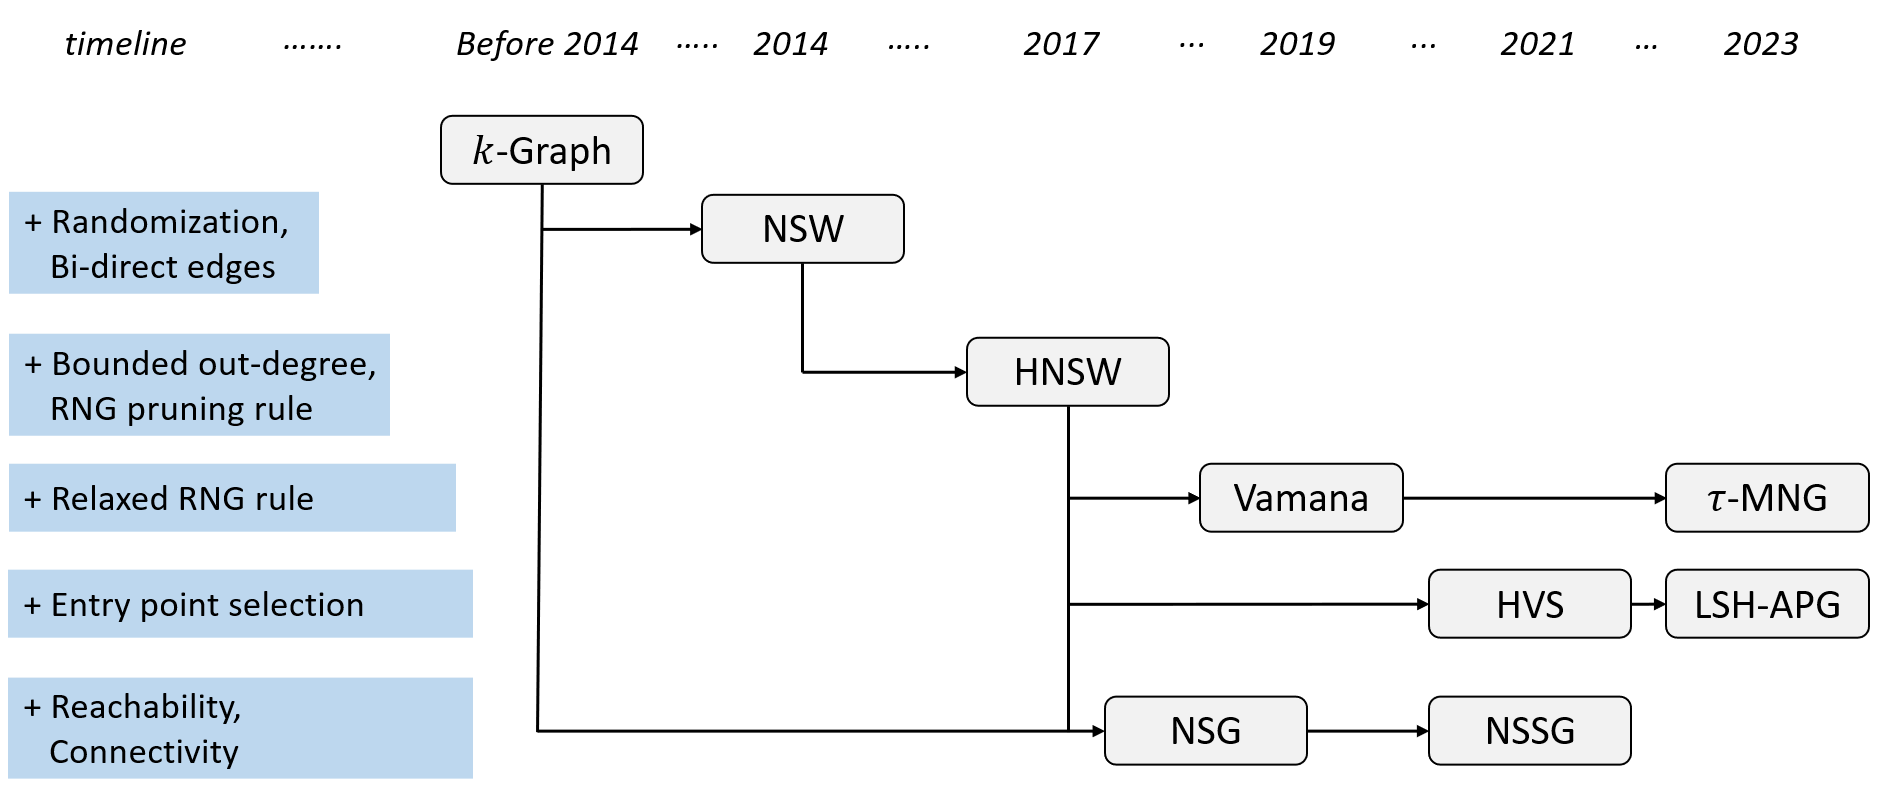
\includegraphics[width=0.8\textwidth]{submissions/Zeyu2023/figs/evo-graph.png}
    \caption{The evolution of the structures of in-memory graph-based indexes. The solid arrows denote the inheritance of designs. }
    \label{zeyu_fig:evo-graph}
\end{figure}

\paragraph{Hierarchical Navigable Small World Graph (HNSW)~\cite{hnsw}}
HNSW has a hierarchical structure where the graph in the lower layer contains all the points in the upper layers and the bottom layer HNSW$_0$ contains all points in the dataset.
The number of points is reduced exponentially bottom-up, and the level of a point is decided randomly.
The query starts from the top layer to find NNs as the entry points of the next layer until reaching the bottom layer.
Like NSW, HNSW is also built by sequential insertion and greedy search, but with a limited out-degree $2M$.
Once a point's out-degree exceeds $2M$, HNSW prunes neighbors using the RNG rule: this is derived from the Relative Neighborhood Graph~\cite{rng}.
Simply speaking, the RNG rule removes the longest edge in the triangles existing in the graph.
In this way, HNSW tries to preserve the reachability of the graph index while limiting the out-degree, by removing the ``redundant'' edges, at the expense of a few more hops when querying.

\paragraph{Relaxed pruning rule: Vamana~\cite{diskann} and $\tau$-MNG~\cite{tau}}
Since the heuristic RNG pruning rule tends to be ``strict'', recent studies have verified that some useful edges are also pruned, which leads to a sub-optimal graph structure.
Vamana relaxes the RNG rule by allowing the inclusion of the longest edge in a triangle, if it is not $1+\alpha$ times longer than the second longest edge, where $\alpha$ is a user-defined relaxing parameter.
In this way, Vamana shortens the search path when querying, which helps reduce random I/Os when the index is on disk.
A recent study~\cite{tau} points out that RNG rule is ineffective when the query does not belong to the dataset, and mitigates this problem by relaxing the RNG pruning rule with a parameter $\tau$.
We omit the details for lack of space.
The resulting approach, $\tau$-MNG, is expected to have a lower search time complexity than other graph-based indexes when the distance between the query and its nearest neighbor is smaller than $\tau$. 
% relaxes the RNG rule by a parameter $\tau$, where if the distance between two points is smaller than $3\tau$, they must connect to each other and for farther points the occlusion area is also narrowed.
% $\tau$-MNG is expected to have better navigability where each step in the search route is closer to the query by $\tau$ under some circumstances.

\paragraph{Better entry points: HVS~\cite{hvs} and LSH-APG~\cite{lsh-apg}}
HVS and LSH-APG use auxiliary data structures to obtain better entry points for the graph-based indexes.
HVS leverages an adaptive hierarchical tree index with quantization techniques, while LSH-APG builds multiple LSB-trees for coarse-grained indexing.
The graph-based index is HNSW$_0$~\cite{hvs}, or even a simpler variant~\cite{lsh-apg}.

\paragraph{Better reachability: NSG~\cite{nsg} and NSSG~\cite{nssg}}
Although HNSW achieves prominent \emph{average} query performance, it cannot guarantee the reachability to any point in the graph index.
Since accomplishing the reachability starting from any point in the graph is intractable, recent graph-based indexes opt to fix the entry point(s) and guarantee the reachability from these entry points.
NSG uses the medoid point of the dataset as the entry point, and refines $K$-Graph to ensure reachability.
Specifically, for a specific point $v$, NSG regards $v$ as a query and performs approximate greedy search in the graph index.
The visited points during the search (along with the neighbors of $v$ in $K$-Graph) become the candidate neighbors of $v$, and are then pruned by RNG rule to limit the out-degree.
After iterating all the points, NSG tests the reachability with a Deep-First-Search Tree rooted at the entry point.
The isolated points will be linked by the nearest point in the tree.
In contrast to NSG, NSSG randomly selects a group of points as entry points, and only uses two-hop neighbors of a point in $K$-Graph as the candidates of neighbors for pruning.
Besides the reachability to the point in the dataset, NSSG also considers the points that do not belong to the dataset, by studying the trade-off between the navigability and the sparsity of the graph index under the RNG rule.
% NSG extends the candidate neighbors by searching $k$NN on existing graphs and uses the RNG rule to prune neighbors like HNSW.
% Furthermore, to ensure connectivity, NSG performs a DFS from the entry point as the root node and adds a link for the point that cannot be reached from the nearest neighbors of the point in the DFS-Tree.~\footnote{todo: decompose}
% In contrast to NSG, NSSG takes two-hop neighbors in $K$-Graph as candidates and tries to add reversed edges for more long-range connections.

\subsection{Understanding the Evolution with Ablation Studies}
Although the heuristics of advanced graph-based indexes have been stated in the papers, it is yet not clear why the proposed techniques work well.
In this subsection, we describe the evolutionary process from $K$-Graph to NSW, HNSW and more optimizations on HNSW by abundant ablation studies.
We aim to help readers understand which techniques actually enhance the performance and the reasons behind their effectiveness from a novel perspective, which can inspire the future designs of ANNS algorithms.

\subsubsection{The problem of $K$-Graph}
\label{zeyu_sec:k-graph}
\begin{wraptable}{r}{0.36\textwidth}
        \centering
        \footnotesize
    \caption{Skewness of in-degree distribution of graph-based indexes}
    \label{zeyu_tab:skewness}
    \begin{tabular}{ccc}\\
    \toprule
              & Deep1M & SIFT1M \\ \midrule
    $K$-Graph & 2.436  & 1.875  \\ \midrule
    NSW       & 4.642  & 4.107  \\ \midrule
    pNSW      & 4.025  & 3.457  \\ \midrule
    HNSW$_0$   & 1.209  & 1.395  \\ \bottomrule
    \end{tabular}
\end{wraptable}
We start by examining the $K$-Graph approach, because not only $K$-Graph is a graph-based index, but it also exhibits some inherent properties (detailed below) of high-dimensional vectors in the context of ANNS problem. 
In this paper, we use \emph{exact} $K$-Graphs instead of approximate ones to avoid the effect of approximation errors.
A common argument in the literature for the unsatisfactory query performance of $K$-Graph is the loss of navigability~\cite{hnsw,wang-survey}, which is verified on real datasets in ~\cite{k-regular}.
However, it is not yet clear the root cause of the loss of navigability.
According to previous studies, the distribution of in-degree of points is very skewed~\cite{hub}.
That is, a small portion of points occupy most of the $k$NN lists for all the points while most of the other points are rarely linked by others.
This is also verified by our experiments on real datasets as shown in Table~\ref{zeyu_tab:skewness} with skewness (standardized third moment).
For simplicity, we denote the in-degree of a point in $K$-Graph by $k$-occurrence~\cite{hub}.
Note that $k$-occurrence is a property of a point in a dataset, independent of the type of index built on the dataset.

Furthermore, we observe that in $K$-Graph the points with high in-degree (i.e., hubs) always interconnect with each other.
To describe this phenomenon, we define the out-link density of a group of points $X\subset V$ as $\rho_{out-link}(X) = \frac{|\{(x,y)|x, y\in X \wedge (x,y)\in E\}|}{|\{(x,y)|x \in X \wedge y \in V \wedge (x,y)\in E\}|}$.The out-link density describes how much a group of points is interconnected.
A high out-link density means these points tend to connect to themselves rather than other points in the graph.
In Figure~\ref{zeyu_fig:outlink-density}, we select different number of hubs and compute the average out-link density of these hubs.
The baseline is a random graph, where each point has $K$ out-neighbors selected uniformly at random. 
As we can see, the out-link density of the hubs in $K$-Graph is much higher than the random graph and NSW.
Over half of the out-links of the 5\% hubs connect to themselves instead of other points.
\begin{wrapfigure}{r}{0.64\textwidth}
    \centering
    \subfloat[Deep1M]{
    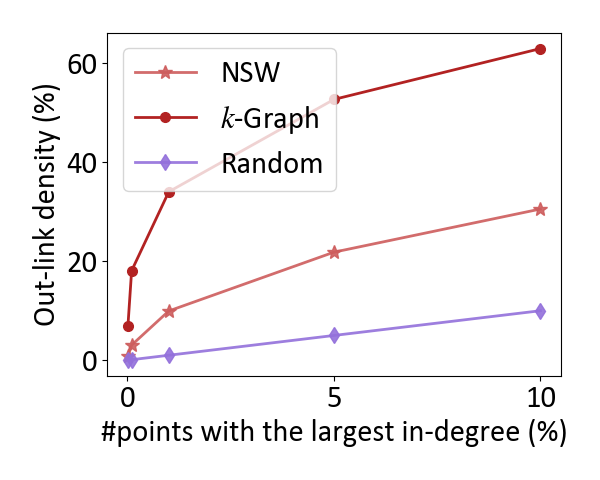
\includegraphics[width=0.32\textwidth]{submissions/Zeyu2023/figs/deep-outlink-density.png}
    \label{zeyu_fig:outlink-density-deep}
    }
    \subfloat[Sift1M]{
    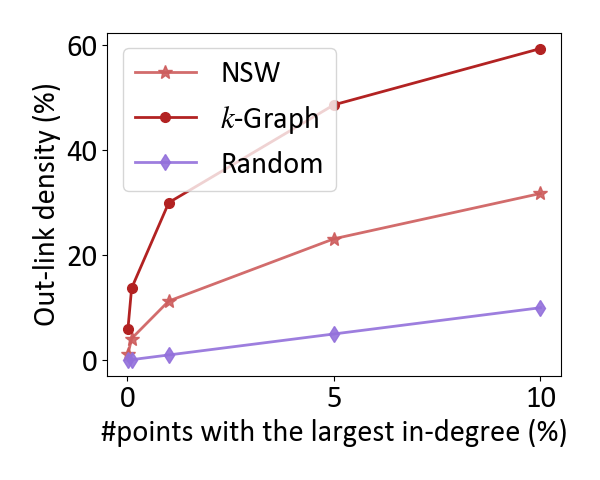
\includegraphics[width=0.32\textwidth]{submissions/Zeyu2023/figs/sift-outlink-density.png}
    \label{zeyu_fig:outlink-density-sift}
    }
    \caption{Out-link density of the group of points with the largest in-degree.}
    \label{zeyu_fig:outlink-density}
\end{wrapfigure}

This phenomenon leads to local optima in $K$-Graph, which is a classical problem of the greedy search algorithm.
Consider an extreme case where $ef=1$ for querying, i.e., $Res$ only contains the nearest checked point to the query, which means that the points further than the current visited point will never be visited.
In other words, no backtracking exists in the search route.
In this case, if the search route steps into a point which is closer to the query than all its neighbors, the search algorithm terminates directly, as shown in Figure~\ref{zeyu_fig:local-optimum}, and the actual nearest neighbors (that could be reached by detouring) are missed.
The termination point is a local optimum, in contrast to the global optimum (i.e., real $k$NN).
\begin{wrapfigure}{r}{0.36\textwidth}
    \centering
    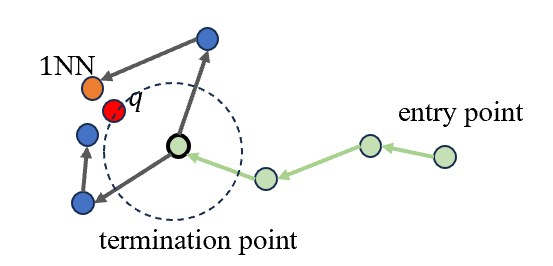
\includegraphics[width=0.36\textwidth]{submissions/Zeyu2023/figs/local-optimum.png}
    \caption{An example of local optimum in the greedy search algorithm.}
    \label{zeyu_fig:local-optimum}
\end{wrapfigure}
Since in $K$-Graph, most of the out-neighbors of a hub are also hubs, once the search route steps into one hub, it is hard to escape from the local optimum to other regions, which may actually contain the true nearest neighbors.
Worse still, the hubs are frequently visited when querying since the points with high in-degree have a higher probability to be visited when starting from a random point.
As a result, $K$-Graph shows weak navigability to acquire real $k$NN even with a large $ef$.

We further verify this impact by analyzing the returned results of the greedy search algorithms.
Formally, given a query $q$, we collect the true positive set $S_{TP} = A(q) \cap kNN(q)$, the false positive set $S_{FP} = A(q) - kNN(q)$ and the false negative set $S_{FN} = kNN(q) - A(q)$, and compute the average $k$-occurrence of these point sets, denoted by $k^{occur}_{S_{TP}}$, $k^{occur}_{S_{FP}}$ and $k^{occur}_{S_{FN}}$, respectively.
% Recall that the properties on $K$-Graph, as we mentioned at the beginning, are at the same time the properties of the distribution of the data.
In the experiments, we use the same query algorithm and the same sparsity of the graphs with $K$=32 for $K$-Graph and $M$=16 for the other three.
As shown in Table~\ref{zeyu_tab:query-analyses}, for $K$-Graph, the difference between $k^{occur}_{S_{TP}}$ and $k^{occur}_{S_{FN}}$ is the largest, indicating that the points with higher in-degree are easier to be recalled whereas the missing points are markedly less connected.
Moreover, the average $k$-occurrence of points in $S_{FP}$ is also higher than $S_{FN}$ for $K$-Graph, and to achieve a higher recall (95\%), $K$-Graph needs the most number of steps compared with other indexes.
These results verify the above inference that the search route in $K$-Graph is prone to get stuck in the local optimum formed by the hubs and thus needs to pay more effort to escape from this trap.

\begin{table}[t]
\centering
\footnotesize
\caption{Average $k$-occurrence of different sets returned by the greedy search algorithm on different graph-based indexes. \#hops are the average number of points visited in the search route. NDC stands for the average Number of Distance Calculations during search, which represents the time cost.}
\label{zeyu_tab:query-analyses}
\begin{tabular}{ccccccccc}\\
\toprule
Dataset              & Accuracy & Index    & $k^{occur}_{S_{TP}}$    & $k^{occur}_{S_{FP}}$    & $k^{occur}_{S_{FN}}$    & $k^{occur}_{S_{TP}} - k^{occur}_{S_{FN}}$ & \#hops & NDC  \\ \midrule
\multicolumn{1}{c}{\multirow{8}{*}[-6.5mm]{Deep1M}} & \multirow{4}{*}[-3mm]{recall@50=0.90} & $K$-Graph & 61.08 & 41.86 & 14.44 & 46.64 & 116 & 1716 \\ \cmidrule{3-9}
\multicolumn{1}{c}{} &          & NSW      & 61.06 & 40.72 & 32.99 & 28.07   & \textbf{57}     & 1709 \\\cmidrule{3-9}
\multicolumn{1}{c}{} &          & pNSW     & 62.15 & 46.36 & 24.66 & 37.49   & 90     & 1379 \\\cmidrule{3-9}
\multicolumn{1}{c}{} &          & HNSW$_0$ & 61.00 & 45.46 & 37.05 & \textbf{23.95}   & 79     & \textbf{1287} \\\cmidrule{2-9}
\multicolumn{1}{c}{}                        & \multirow{4}{*}[-3mm]{recall@50=0.95} & $K$-Graph & 60.38 & 27.30 & 7.62  & 52.76 & 176 & 2319 \\\cmidrule{3-9}
\multicolumn{1}{c}{} &          & NSW      & 60.17 & 28.28 & 19.55 & 40.62   & \textbf{108}    & 2734 \\\cmidrule{3-9}
\multicolumn{1}{c}{} &          & pNSW     & 61.22 & 31.96 & 15.37 & 45.85  & 162    & 2170 \\\cmidrule{3-9}
\multicolumn{1}{c}{} &          & HNSW$_0$ & 60.72 & 32.57 & 24.39 & \textbf{36.33}   & \textbf{108}    & \textbf{1781} \\\cmidrule{1-9} \cmidrule{1-9}
\multirow{8}{*}[-6.5mm]{SIFT1M}                     & \multirow{4}{*}[-3mm]{recall@50=0.90} & $K$-Graph & 53.81 & 28.90 & 11.72 & 42.09 & 386 & 4927 \\\cmidrule{3-9}
                     &          & NSW      & 54.07 & 41.78 & 37.86 & 16.21   & \textbf{70}     & 2015 \\\cmidrule{3-9}
                     &          & pNSW     & 54.98 & 45.44 & 31.84 & 23.14   & 106    & 1690 \\\cmidrule{3-9}
                     &          & HNSW$_0$ & 54.18 & 44.40 & 40.10 & \textbf{14.08}   & 71     & \textbf{1336} \\\cmidrule{2-9}
                                            & \multirow{4}{*}[-3mm]{recall@50=0.95} & $K$-Graph & 52.86 & 37.27 & 17.17 & 35.69 & 423 & 5336 \\\cmidrule{3-9}
                     &          & NSW      & 54.03 & 32.77 & 27.71 & 26.32   & 112    & 2881 \\\cmidrule{3-9}
                     &          & pNSW     & 54.55 & 35.59 & 23.01 & 31.54   & 169    & 2464 \\\cmidrule{3-9}
                     &          & HNSW$_0$ & 54.03 & 34.04 & 29.70 & \textbf{24.33}   & \textbf{108}    & \textbf{1890}\\\bottomrule
\end{tabular}
\end{table}


Recall that the problems of $K$-Graph is an intrinsic problem for all graph-based indexes on high-dimensional data.
% The dilemma is between local proximity and global navigability.
On the one hand, the local proximity of $K$-Graph is crucial in the recall stage during the search process~\cite{note}.
On the other, over-rich local connections in the graph lead to more local optimum which hinders the search accuracy.
% The global navigability can be achieved by diversified edges in different lengths and directions, which however, turn to be burdens on the recall stage.
% In the following, we will show how the following works face this dilemma and improve the overall performance of the index. 
\begin{table}[tb]
\begin{minipage}{.4\linewidth}
    % \centering
    \footnotesize
        \caption{Pearson correlation coefficients between in-degree and insertion-order/$k$-occurrence of points on different indexes.}
    \begin{tabular}{ccccc}\\
\toprule
& \multicolumn{2}{c}{Deep1M} & \multicolumn{2}{c}{Sift1M} \\\midrule
& Ins. ord.     & $k$-occur.    & Ins. ord.     & $k$-occur.    \\\midrule
$K$-Graph & 0.00  & 1.00 & 0.00 & 1.00  \\ \midrule
NSW       & -0.53  & 0.56 & -0.53 & 0.56  \\ \midrule
pNSW      & -0.44  & 0.68 & -0.43 & 0.67 \\ \midrule
HNSW$_0$   & -0.63  & 0.22 & -0.52 & 0.26  \\ \bottomrule \\
\end{tabular}
    \label{zeyu_tab:corr}
\end{minipage}%
\hspace{6mm}
\begin{minipage}{.31\linewidth}
    \centering
    \footnotesize
    % \scriptsize
     \caption{Query analyses under recall@1=99\%, on different graph-based indexes.}
\begin{tabular}{cccc}\\
\toprule
 \multicolumn{2}{c}{Deep1M} & \multicolumn{2}{c}{Sift1M} \\\midrule
 \#hops     & NDC    & \#hops     & NDC  \\\midrule
  5001  & 29315 & 2047 & 17698  \\ \midrule
        137  & 3244 & 150 & 3644  \\ \midrule
      156  & 3074 & 663 & 7246 \\ \midrule
    156  & 2422 & 111 & 1943  \\ \bottomrule \\
\end{tabular}   
    \label{zeyu_tab:high-recall}
\end{minipage}%
\hspace{2mm}
\begin{minipage}{.22\linewidth}
    \centering
    \footnotesize
    % \scriptsize
\caption{Graph quality of different indexes, where $K$=32 and $M$=16}
\begin{tabular}{cc}\\
\toprule
          Deep1M & Sift1M \\ \midrule
          GQ & GQ \\\midrule
 100\%  & 100\%  \\ \midrule
 51.84\%  & 53.76\%  \\ \midrule
51.82\%  & 52.71\%  \\ \midrule
30.80\%  & 32.17\%  \\ \bottomrule \\
\end{tabular}
    \label{zeyu_tab:graph-quality}
\end{minipage}%
\end{table}

\subsubsection{The Benefit of Long-range Connections}

%Traditional view is small-world graph
% But now we explain it from the hubness
% more tractbale, more comprehensive
% provide a novel view to understand it
% overcome hubness is not easy: recall stage and trap
% conclusion: randomize incur long edges
To mitigate the problem of $K$-Graph, NSW introduces long-range connections to break the traps formed by hubs, and enhance global navigability.
The long-range connections can be defined as the edges that do not exist in the $K$-Graph (whose graph sparsity is similar to NSW).
NSW introduces these connections by randomization.
Recall that when inserting a point, NSW finds its nearest neighbors by greedy search on the \emph{existing} graph, and then builds bi-directional links with these neighbors.
In this way, the degree~\footnote{Note that in NSW, the \emph{in-degree} of a point is equal to its \emph{out-degree} since all edges are bi-directional. Thus, we simply use the term \emph{degree}.} of points in NSW is significantly influenced by the insertion order: the points inserted earlier have a higher possibility to be linked by other points than the later ones.
This is demonstrated in Table~\ref{zeyu_tab:corr}, where the NSW (second line) Pearson correlation coefficients for $k$-occurrence and insertion order are (almost) the same.  
Given that the insertion order is usually random, the lengths of the new links introduced in NSW also tend to be random.
Thus, long-range connections are introduced.

We quantify the size of long-range connections by graph quality~\cite{k-regular,wang-survey}, which is defined as the overlapping ratio of edges with $K$-Graph under similar sparsity.
As shown in Table~\ref{zeyu_tab:graph-quality}, NSW preserves nearly half of the short edges belonging to $K$-Graph, while introducing long-range connections for the other half.
Although affected by the random selection of the previously inserted points, these connections can substantially improve the navigability of graph indexes, as we explain below.
We note that the hubs do not necessarily have high $k$-occurrence, but are also determined by the insertion order.
In other words, the distribution of hubs is ``disrupted'' by randomization.
As a result, the hubs in NSW are not interconnected, and the out-link density of hubs significantly drops compared to $K$-Graph (see Figure~\ref{zeyu_fig:outlink-density}).
It means that although the hubs are still visited frequently, the cases of local optimum are reduced and thus the navigability on NSW is enhanced.
% In contrast to $K$-Graph where the in-degree only relates to $k$-occurrence as defined, in NSW, the insertion order has nearly the same influence as $k$-occurrence on the in-degree of nodes, as shown in Table~\ref{zeyu_tab:corr}.
% Since the insertion order is random in NSW, it can be viewed that the influence of hubness is ``disrupted'' by randomization.
% As a result, the new hubs in NSW are not necessarily close to a large number of points.
% Also, in Figure~\ref{zeyu_fig:outlink-density}, we can see a significant drop from $K$-Graph to NSW w.r.t. out-link density, which means the interconnection of the hubs is weakened.
% In this way, NSW breaks the local optimum formed by the hubs and enhances the navigability.

% In addition, NSW also preserves the local proximity by adding the reversed edges.
% It can be proved that the bi-directional $k$NN of a point $v$, defined as $\{x|x\in kNN(v) \wedge v\in kNN(x)\}$, will be $v$'s neighbors in NSW, {\color{red}under the assumption that the greedy search during constructing NSW is accurate}.

% {\footnote{todo: what does this paragraph mean? it's not clear}}
% Table~\ref{zeyu_tab:graph-quality} shows that the graph quality~\cite{wang-survey,k-regular}~\footnote{todo:add definition of graph quality} of NSW is over 50\%, indicating that over half of the edges in $K$-Graph are preserved in NSW.
Table~\ref{zeyu_tab:query-analyses} shows that in order to achieve the same recall, NSW needs on average only \textbf{32}\% of the $K$-Graph steps.
The difference between $k^{occur}_{S_{TP}}$ and $k^{occur}_{S_{FN}}$ is reduced by half, clearly demonstrating that the missing nearest neighbors are less susceptible to local optima, and leading to performance improvements. % beyond $K$-Graph on some settings, verifying our analyses beforehand.
In some cases though, e.g., in the Deep1M dataset, the improvement is marginal and even negative, despite the short search paths.
The reason is that the degree of NSW is not fixed.
Since the search cost of the greedy search algorithm is the product of the length of the search route and the out-degree of each point in the route, a high out-degree will linearly increase the time complexity.
Worse still, the distribution of degree of points in NSW is even more skewed than $K$-Graph (see Table~\ref{zeyu_tab:skewness}), which further degrades the worst-case time complexity.

% not necessarily with low $k$-occurrence; NSW is not trapped by interconnected hubs, despite that the search algorithm still shows bias on points with high $k$-occurrence.

% {\footnote{todo: pNSW is for the benefit of long-range connections}}
% Although NSW provides better navigability than $K$-Graph, a nice property that {\footnote{todo:rewrite}} the out-degree of each node is fixed, is violated.
% It leads to the distribution of out-degree (equally to in-degree) is severely skewed in NSW, as shown in Table~\ref{zeyu_tab:skewness}.
% Since the search cost of the greedy search algorithm is the product of the length of the search route and the out-degree of each point in the route, a high out-degree will linearly increase the time complexity.
% {\footnote{todo: why NSW is not good, table 2}}

A simple optimization is to restrict the out-degree to $2M$ by selecting the nearest $2M$ neighbors.
We call this method pruned-NSW (pNSW).
pNSW mainly removes the long-range connections, which can be verified by the fact that the graph quality is nearly the same as NSW (see Table~\ref{zeyu_tab:graph-quality}).
% The graph quality of pNSW is nearly the same as NSW (see Table~\ref{zeyu_tab:graph-quality}), verifying that the local proximity remains unchanged.
As shown in Table~\ref{zeyu_tab:query-analyses} pNSW seems have a better performance than NSW by sacrificing a little navigability and achieves a remarkable gain in overall performance.
However, as shown in Table~\ref{zeyu_tab:high-recall}, under high-recall constraint (99\% recall@1), pNSW suffers a significant degradation on Sift1M dataset, nearly two times slower than NSW.
The results of pNSW further demonstrate that the long-range connections, especially the links of the hubs, significantly influence the global navigability of the graph index.
% It results from the reduction of long-range links.
% However, the reduction of long-range links, especially the links coming from the hubs, significantly impairs global navigability.
% \begin{wrapfigure}{r}{0.38\textwidth}
%     \centering
%     \includegraphics[width=0.38\textwidth]{figs/triangle.png}
%     \caption{Tree design principles of graph-based indexes.}
%     \label{zeyu_fig:triangle}
% \end{wrapfigure}

% The results of pNSW inspire us that an efficient graph-based index 
% Therefore, the technical challenge lies in the triangle that what will be the optimal edge allocation strategy that satisfies local proximity, global navigability and low out-degree at the same time, as shown in Figure~\ref{zeyu_fig:triangle}.
% To overcome this challenge, it is intuitive to satisfy the low out-degree by a fixed parameter, and then balance the local proximity and navigability given the limited edge budget.

\subsubsection{The RNG Pruning Rule}
Up to this point, there seems to exist a tradeoff in the design of graph indexes between search efficiency and navigability.
If we limit the (out-)degree of points for efficiency, navigability will be hurt, as in $K$-Graph and pNSW.
If we break the degree limit, the search efficiency will degrade, as in NSW.
To address this situation, we observe that the distribution skewness of the points' in-degree is a key point.
A skewed distribution means the existence of hubs in the graph, and given the high visit frequency of these hubs, these hubs bear the responsibility of high navigability.
In order to provide navigability, hubs need a high degree and more long-range connections, causing the problem mentioned above.
Therefore, if we can render in-degree distribution less skewed, then hubs will no longer exist and the navigability will be provided equally by all the points in the graph.
In this case, the bounded degree and the navigability can be achieved at the same time.

HNSW is a nice example of this rationale.
Given that the skewness of the $k$-occurrence distribution is an inherent property of high-dimensional vectors, ``amortizing'' the navigability to all points is very challenging.
HNSW leverages two techniques to accomplish this target.
One is randomization, like NSW, which disrupts the distribution of hubs.
The other is RNG pruning rule, which is a key design inherited by most of the following graph-based techniques~\cite{nsg,nssg,wang-survey}.
Specifically, for a point $v$ to be inserted, HNSW first collects sufficient nearest neighbors on the existing graph as candidates by greedy search, and then prunes these candidate neighbors down to $M$, using the RNG rule.
Finally, like NSW, HNSW tries to add $M$ reversed links from the $M$ selected neighbors to $v$.
Once the reversed link exceeds the out-degree limit $2M$, the RNG rule will be used to prune these neighbors to no more than $2M$.
For clarity, we only consider HNSW$_0$ in this section to avoid the influence of the hierarchy, which will be discussed separately in the next section.

When pruning candidate neighbors, HNSW sorts them according to the distance to the inserted point $v$ and checks them in order.
The inserted neighbor $c$ should satisfy that $\forall c'\in C(v), dist(v,c)<dist(c,c')$, where $C(v)$ is the set of already selected neighbor points. 
Consider the example in Figure~\ref{zeyu_fig:rng} (left), where $C=\{c_1,c_2\}$.
The next candidate neighbor $c$ will be pruned, because $dist(v,c)>dist(c,c_2)$.
The heuristic behind the RNG rule is that for the pruned neighbors like $c$, even though $v$ does not directly link to $c$, $v$ can reach $c$ by detouring from $c_2$.
Since $c_2$ is closer to $c$, $v$ must not be the local optimum if the query is on, or near to $c$.
As a result, compared to NSW, HNSW filters out many of the $M$ nearest neighbors found during the greedy search, without losing the reachability to them~\footnote{This is not strict since there is no guarantee on the existence of edge ($c_2,c$).}.
In this way, the saved slots of out-neighbors can be used to accommodate more long-range connections. 
As shown in Table~\ref{zeyu_tab:graph-quality}, only about 30\% of the edges in $K$-Graph are preserved in HNSW. 

\begin{wrapfigure}{r}{0.36\textwidth}
    \centering
    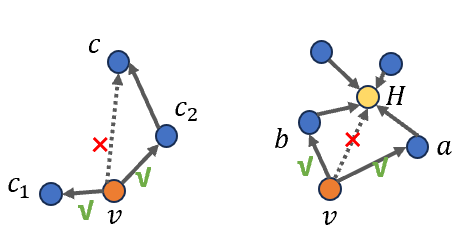
\includegraphics[width=0.36\textwidth]{submissions/Zeyu2023/figs/rng.png}
    \caption{RNG rule.}
    \label{zeyu_fig:rng}
\end{wrapfigure}


Besides pruning some ``unnecessary'' edges, the RNG rule also helps mitigate the skewness of in-degree distribution for high-dimensional vectors.
Specifically, the points with high $k$-occurrence tend to reject more in-links from other points because of the RNG rule.
Consider the example in Figure~\ref{zeyu_fig:rng} (right), where $C(v)=\{a,b\}$, and the candidate neighbor $H$ has been linked by some points because of closeness.
In this case, $H$ will be pruned since it can be reached indirectly from $a$ and $b$.
This example indicates that if a point is close to many other points (i.e., points with high $k$-occurrence like $H$), it has to ``compete'' against these close points for becoming the neighbor of an inserted point.
Naturally, the probability of building links with such points is lower than the point with low $k$-occurrence.
This is exactly the opposite to the linking strategy of the $K$-Graph index.
As shown in Table~\ref{zeyu_tab:corr}, the correlation coefficient between the in-degree and $k$-occurrence for HNSW is less than 0.3, indicating a very weak correlation.
As a result, the inherent skewness of the in-degree distribution of high-dimensional vectors is optimized by the RNG rule: the skewness value drops to nearly a half when compared to $K$-Graph, as shown in Table~\ref{zeyu_tab:skewness}. 
% In this way, the difference of visit frequency among the points in the graph is not outstanding and the navigability is achieved by all the points. 
Moreover, for every point in HNSW, there exists a sufficient number of short edges for local proximity, but also enough long-range connections for global navigability, which ensure the query efficiency in the recall and navigation stage respectively.
As shown in Tables~\ref{zeyu_tab:query-analyses} and~\ref{zeyu_tab:high-recall}, even though HNSW has a limited out-degree, it uses a similar number of steps to NSW in order to reach a low/high recall.
This demonstrates that the RNG rule successfully preserves the navigability in these datasets.
As for the overall query performance, HNSW always achieves the best results (well ahead of the second best), across all settings.  

% and the current point $x$ that regards $H$, $a$ and $b$ as candidates of neighbors.
% When selecting neighbors, the nearest $a$ is first selected and then $b$ is also selected since $b$ is closer to $x$ than to $a$.
% The third candidate is $H$, which will be rejected since $x$ can already access $H$ by $a$ or $b$.
% In addition, RNG rule also effectively mitigates the skewness of the in-degree distribution, a significant drop as shown in Table~\ref{zeyu_tab:skewness}.
% Specifically, the points with high $k$-occurrence tend to reject more in-links from other points due to RNG rule.
% As we have described in Section~\ref{zeyu_sec:k-graph}, the hubs are usually close to many other points.
% Consider the point $H$ in Figure~\ref{zeyu_fig:rng} that has been linked by some points, and the current point $x$ that regards $H$, $a$ and $b$ as candidates of neighbors.
% When selecting neighbors, the nearest $a$ is first selected and then $b$ is also selected since $b$ is closer to $x$ than to $a$.
% The third candidate is $H$, which will be rejected since $x$ can already access $H$ by $a$ or $b$.
% Therefore, more old hubs from $K$-Graph are removed, and the points far from the center, in a relative sense, obtain more opportunities to absorb links from other points.
% This result is consistent with our inference above that achieving low out-degree and navigability requires less skewed distribution and fewer hubs.
% As a result, HNSW allows more effective long-range connections for navigability (see Table~\ref{zeyu_tab:high-recall}), and preserves the efficiency in the local recall stage (see Table~\ref{zeyu_tab:query-analyses}).




% An inspiration from pNSW is that once the out-degree is bounded, the navigability of any point in the graph is also bounded, including the hubs that provide the function of navigability in NSW.
% To overcome the trade-off between low out-degree and navigability, a latent requirement is that the skewness of in-degree distribution should be weakened.
% In this case, the function of navigability should be transferred equally to all the points in the space, that is, the hubs no longer exist.

% \footnote{todo: HNSW does what I say before}
% In HNSW, the RNG-based pruning rule is used to remove unnecessary edges in the graph, especially in the local neighborhood of a point, and thus leaves more space for long-range connections.
% The core technique of HNSW is the RNG-based pruning rule (RNG rule for short).
% \footnote{todo: cannot get why short edges are removed}
% Simply speaking, given the nearer neighbors are considered first, RNG rule removes the longest edge in any triangle of the graph, as shown in Figure~\ref{zeyu_fig:rng}.
% ~\footnote{rewrite the follwing sentence}
% The heuristic is that the current node, though cannot visit the removed neighbors directly, can access them by a hop of existing neighbors.
% In this way, HNSW preserves the local proximity with much fewer edges, about 30\% of slots as shown in Table.~\ref{zeyu_tab:graph-quality} at the cost of several additional hops.
% The same heuristic also holds for the pruning of long-range links, allowing longer and diversified connections to enhance navigability.



\subsubsection{Hierarchy and Selection of Entry Points}
The classical hierarchical index structure of HNSW is widely employed in both research and industrial settings~\cite{k-regular,diskann,nsg,milvus}.
Intuitively, the upper layers in HNSW form long-range connections providing navigability, while the bottom layer uses small-range links to cover ``the last mile''.
However, we claim that this strategy does not provide any significant benefits in the case of high-dimensional spaces.
As shown in Figure~\ref{zeyu_fig:ablation}, using HNSW$_0$ (the bottom layer of HNSW) alone, leads to nearly the same query performance as (the original, hierarchical) HNSW. 
This result, which is verified on a dozen of public datasets (omitted due to lack of space) as well as by other studies~\cite{promise}, casts some doubt about the usefulness of the hierarchical structure.
We make the following two observations that try to explain the above result:
% \begin{itemize}
(i) Due to the distance concentration phenomenon~\cite{dist-concentrate}, the query is not far away from a random point in the same dataset.
For example, in Sift1M and Deep1M datasets, the average distance between a random point and the query is merely \textbf{5.3}x and \textbf{3.5}x, respectively, larger than the average length of the short edges in $K$-Graph.
(ii) The bottom layer can provide the navigability necessary to quickly approach the local neighborhood.
For example, to achieve 99\% recall@1, HNSW$_0$ needs 111 hops on the Sift1M dataset, compared to 108 hops for HNSW; on Deep1M, HNSW$_0$ needs 156 hops, compared to 151 hops for HNSW.
These small differences verify the efficient navigability of HNSW$_0$.
% \end{itemize}

% \begin{wrapfigure}{r}{0.3\textwidth}
%     \centering
%     \includegraphics[width=0.3\textwidth]{figs/upper-layer.png}
%     \caption{Quality of entry points in HNSW.}
%     \label{zeyu_fig:upperlayer}
% \end{wrapfigure}
\begin{figure}[tb]
    \centering
    \subfloat[Sift1M]{
    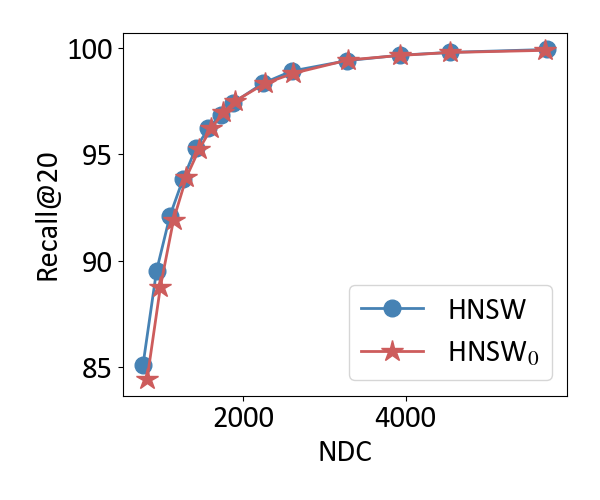
\includegraphics[width=0.33\textwidth]{submissions/Zeyu2023/figs/sift-upper-layer.png}
    }
    \subfloat[Deep1M]{
    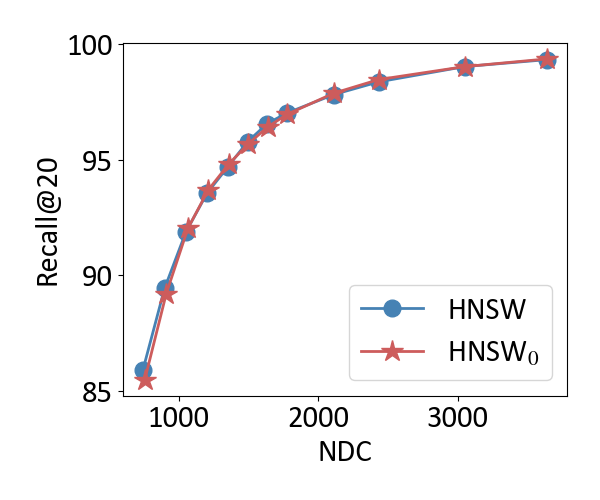
\includegraphics[width=0.33\textwidth]{submissions/Zeyu2023/figs/deep-upper-layer.png}
    \label{zeyu_fig:ndc-deep}
    }
    \subfloat[Deep10M]{
    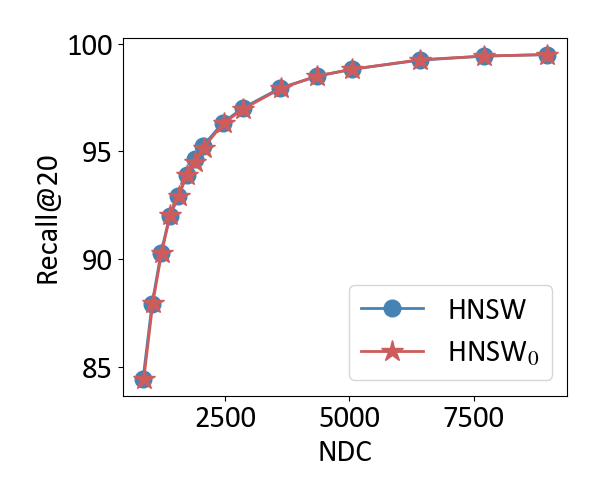
\includegraphics[width=0.33\textwidth]{submissions/Zeyu2023/figs/deep10M-upper-layer.png}
    \label{zeyu_fig:ndc-deep10M}
    }
    \caption{The query performance of HNSW and HNSW$_0$: the difference is negligible.}
    \label{zeyu_fig:ablation}
\end{figure}
In this case, the benefit of the selection of entry points for graph-based indexes relies on the accuracy of the entry points and the cost of obtaining these entry points.
Unfortunately, the upper layers of HNSW do not show an obvious benefit since they only contain a small portion of data.
According to our experiments, only less than half of the queries obtain one of the 50NN in the upper layers, which means that a significant part of the work actually takes place at the bottom layer. 
To break this limit, subsequent works, including HVS~\cite{hvs} and LSH-APG~\cite{lsh-apg} (both discussed earlier), use another index as an auxiliary structure to help obtain high-quality entry points.
% Certainly, the auxiliary index contains all the points of the dataset and is able to quickly acquire approximate $k$NN which are good enough to act as the entry points for HNSW$_0$.
The quality of entry points is largely improved, and as reported, HVS achieves over 3x faster query answering time than HNSW on hard datasets and high recall range, while LSH-APG achieves 1.5x faster query answering time, while offering more efficient index construction.





% \subsubsection{$K$-Graph: Trapped by Clustered Hubs}



\section{Tree-based Index Family}
\label{zeyu_sec:tree}
% basic structure (definition), query algorithms, 
% In this section, we will survey and analyze another important index family for high-dimensional data, the tree-based index family.
The tree-based index family hierarchically partitions the high-dimensional space, which may be transformed or projected, and groups similar vectors in the same partition as leaf nodes.
Usually, the root node of the tree-based indexes covers the whole high-dimensional space and the children nodes of it cover disjoint or overlapped sub-spaces.
When querying, we traverse the tree-based index from the root node to one or more leaf nodes by judging which sub-spaces the query vector belongs to or is close to.
Then the data inside these leaf nodes are candidates of $kNN$.
In this section, we will survey the latest tree-based indexes proposed in the past five years and summarize the evolution in Figure~\ref{zeyu_fig:evo-tree}.
It can be viewed as an extension of the previous survey of tree-based indexes~\cite{evolution}.
% We summarize there are three main directions that recent progress of tree-based indexes lie on, including optimized index structure, parallel and distributed execution.

\subsection{Preliminaries and Overview}
The designs of tree-based indexes (in a single machine) can be decomposed into three parts, including data summarization (i.e., dimension reduction), indexing, and querying algorithms.
In this subsection, we briefly describe the preliminaries of these techniques leveraged in recent works.

\paragraph{iSAX-index family}
iSAX summarization is a dynamic prefix of SAX words~\cite{sax}, and SAX is a symbolization of Piecewise Aggregate Approximation (PAA for short).
PAA represents a vector with the means of disjoint equal-length segments, and SAX discretizes PAA with symbols.
iSAX word is a prefix of the corresponding SAX word, which can flexibly represent a sub-space in the reduced space.
Based on iSAX, the iSAX index family~\cite{evolution} organizes data in a tree structure, where each node is summarized by an iSAX word.
The root node covers the whole space and it can be split by refining one segment of its iSAX word.
The children nodes own disjoint sub-spaces of their parent.
When querying, the iSAX word of each node can be used to prune irrelevant data benefiting from that the distance between iSAX summarization lower bounds the actual distance.

\paragraph{EAPCA-index family}
The EAPCA-index family~\cite{dstree} differs itself from iSAX by 1) using dynamic segmentation that is determined on the fly when building index, 2) using mean and standard deviation to represent each segment and thus providing tighter bounds when querying, 3) more splitting choices and adaptive split criteria.

\paragraph{Ordered-index family}
The Ordered-index family~\cite{coconut} sorts high-dimensional data with space-filling curves (e.g., Z-order curve, Hilbert-order curve) and then index them with classical B-tree, etc.
Space-filling curves approximately preserve the proximity between points that are close in high-dimensional space.
The approximation error increases as the dimensionality goes larger.
So usually dimension-reduction techniques are used beforehand.
% However, space-filling curves are not sufficient to describe the proximity on tens, hundreds or more dimensions.
% That is, the points that are close in high-dimensional space are not necessarily close on the space-filling curve in low-dimensional space.
% So before sorting with these curves, other dimension reduction techniques are usually first adopted to reduce data to several dimensions.
% As a result, the search accuracy of ordered-index family depends both on the dimension reduction technique and the following sorting mechanism.

\begin{figure}[t]
\centering
    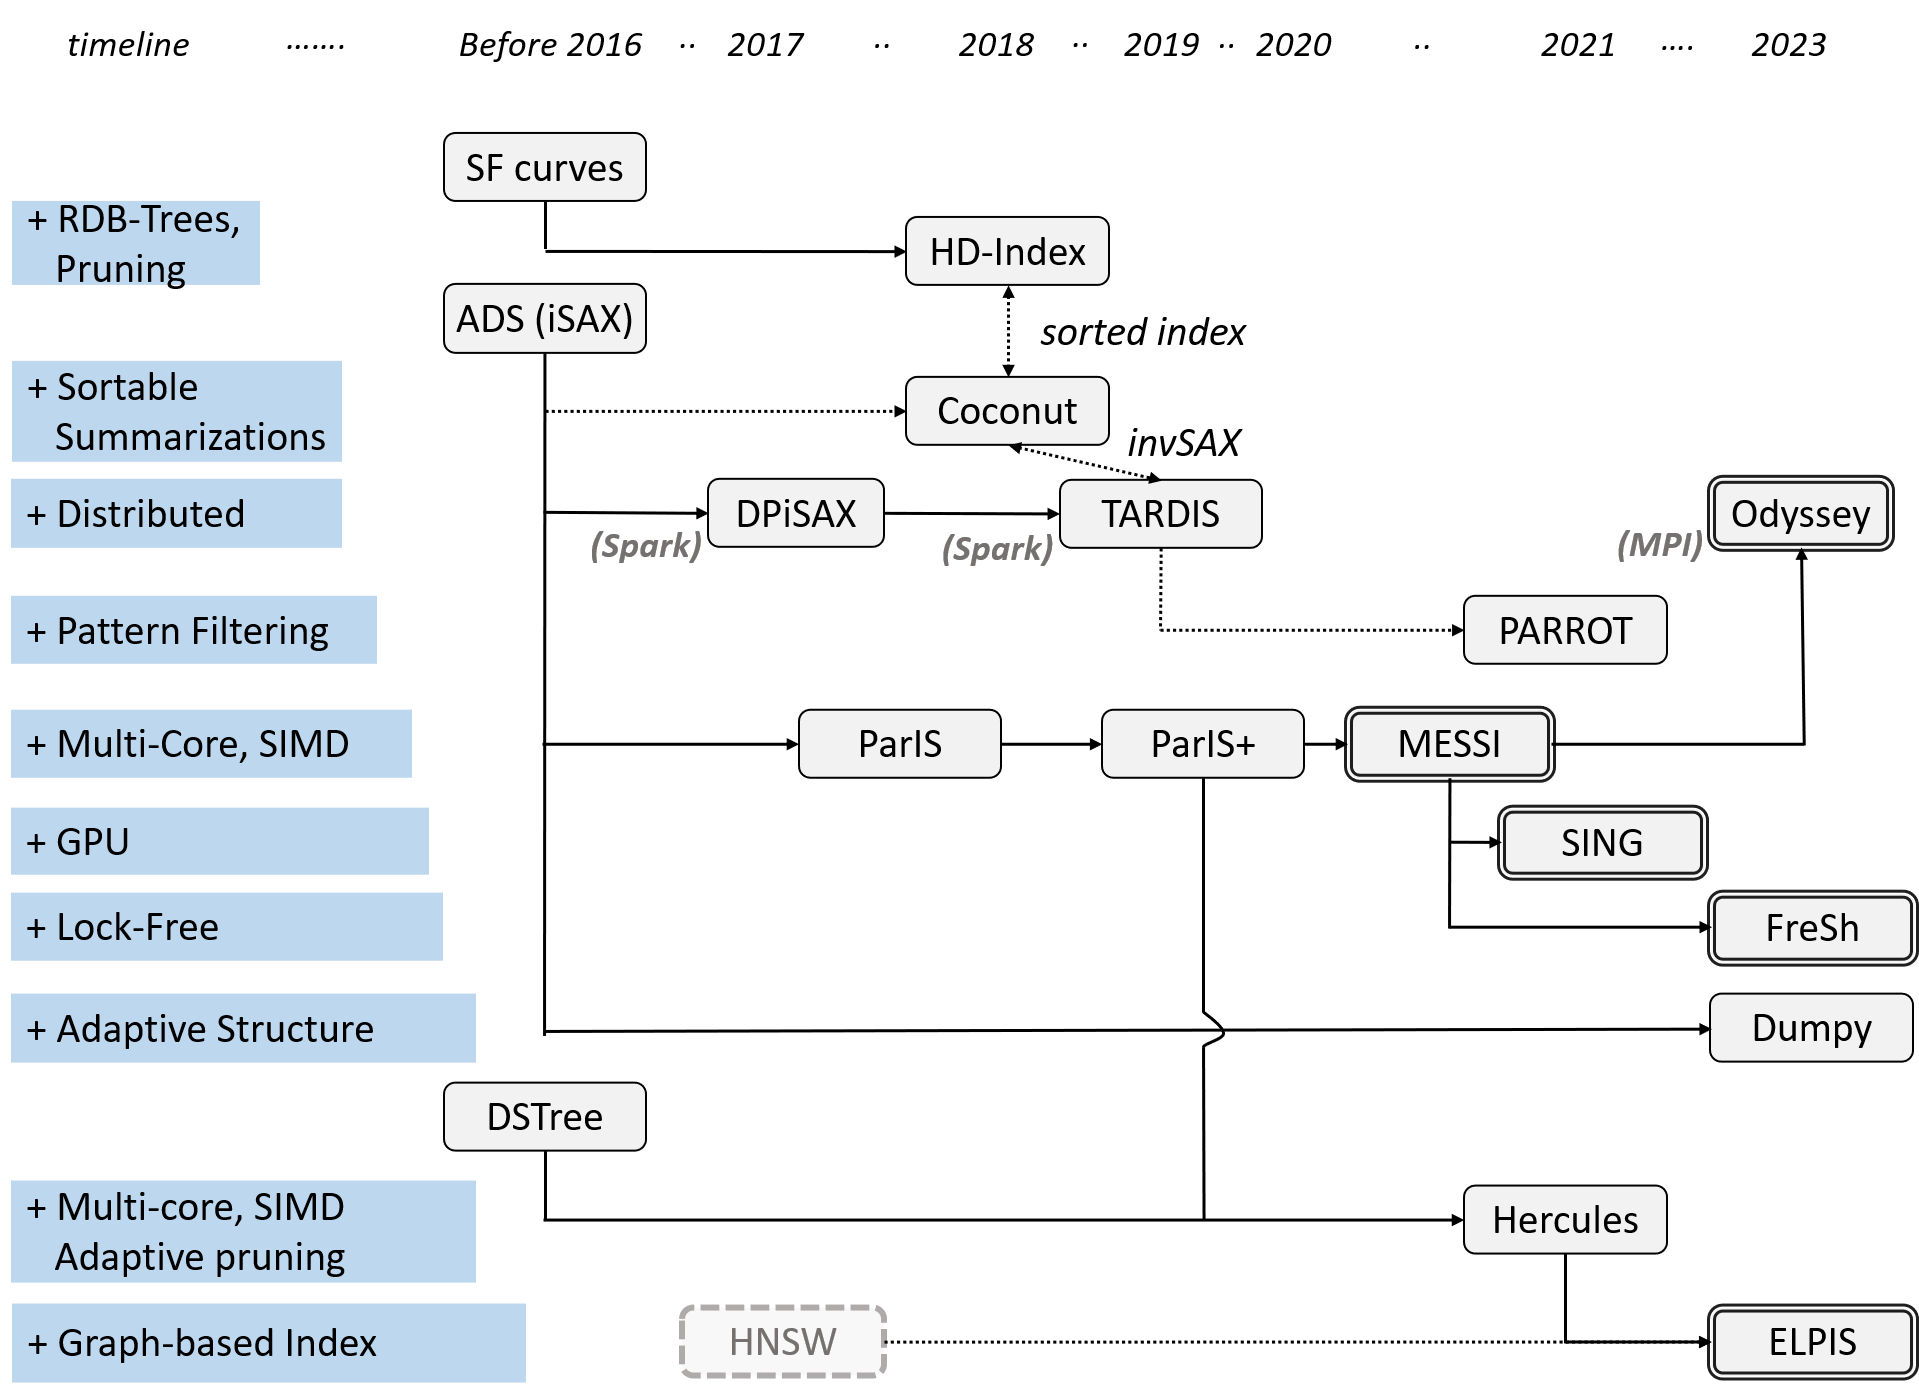
\includegraphics[width=0.8\textwidth]{submissions/Zeyu2023/figs/tree-evo.png}
    \caption{
    %zeyu: add Elpis
    The evolution of tree-based index in the past 6 years, as an extended figure of~\cite{evolution}. The solid arrows denote the inheritance of the index design; the dashed arrows denote the correlation of the design features; indexes in double-lined boxes are in-memory solutions, while the rest are on-disk solutions. Note that HNSW is not a tree-based index; it is included, because ELPIS (discussed in Section~\ref{zeyu_sec:combination}) inherits some of its features.}
    \label{zeyu_fig:evo-tree}
\end{figure}

\subsection{Optimized Disk Index Structure}
Managing large-scale high-dimensional vectors on disk is challenging since the data locality (i.e., similar vectors should be placed together such that they can be fetched by one I/O) and the index quality (i.e., nearest neighbors should be quickly located by the index) should be considered at the same time.
% Most advanced works before the following recent progress, like iSAX2+~\cite{isax2+} need days to index billion-level data and minutes to execute a query.
Recent progress has remarkably advanced the state-of-the-art to hour-level indexing time and ms-level query time on billion-sized datasets.

% zeyu: shortened
\paragraph{HD-Index~\cite{hd-index}.}
HD-Index, as an ordered index, builds multiple B+ trees each of which stores the Hilbert keys of a segment of dimensions.
In this way, HD-Index mitigates the loss of accuracy due to the dimensionality reduction.
To facilitate the refinement, HD-Index randomly places pivots and stores in the index the distance between an entry and the nearest reference point, which provides the ability to prune when querying.
However, the search cost of HD-Index increases linearly with dimensionality, leading to an inefficient solution for very high-dimensional vectors.

% zeyu: I'd like to discuss Coconut again for its prominent merits and defects.
\paragraph{Coconut~\cite{coconut}.}
In contrast to HD-Index which sorts raw (sub)-vectors, Coconut first reduces dimensionality using SAX, and then sorts SAX words by the z-order curve.
In this way, the most significant dimensions (i.e., bits) of the SAX words are considered first.
This process matches exactly the principle of SAX summarization, i.e., coarse-grained partitioning is encoded in the most significant bits, while fine-grained partitioning in the least significant bits. 
Using only one B-tree to index the keys, Coconut has a very fast query time, and the highly packed leaves also lead to a small improvement in the results of approximate search.
%However, as Coconut does not implement any special approximate search algorithm, it is hard to achieve a high recall with a limited number of candidates.

\paragraph{Dumpy~\cite{dumpy}.}
Dumpy is an iSAX-based index designed for high-precision approximate search and fast index-building for large datasets.
Dumpy leverages the trade-off between the proximity inside the leaf node and the compactness (i.e., the fill factor) of these nodes by dynamically selecting the number of segments and which segments to split along according to the data distribution.
It also proposes a leaf node packing algorithm and a vector duplication mechanism that further optimizes the data layout on the index.
As a result, Dumpy can provide high-recall answers with much fewer random I/Os. % with the preserved pruning ability of iSAX.


\subsection{Parallel Processing}
Parallel indexing and querying on the tree-based index is not trivial for dynamic structure and pruning-based query~\cite{paris,messi}.
The difficulties include the reduction of race conditions and load balancing among threads.
The ParIS+ index~\cite{paris}, parallelizes the building and querying algorithms of ADS+~\cite{ads}, an adaptive variant of the iSAX index.
MESSI~\cite{messi} further optimizes the race conditions for in-memory datasets, while SING~\cite{sing} extends the query answering algorithm to make use of GPUs.
In recent years, the research boundary has been pushed by a parallel and fully-materialized disk index, and a novel lock-free parallelism mechanism.


\paragraph{Hercules~\cite{hercules}.}
Hercules is an EAPCA-based parallel disk-based index.
Designed for large-scale datasets, Hercules optimizes memory management with a two-level buffer model to reduce the time cost of memory management.
Besides that, Hercules delicately schedules different tasks with a given number of threads, resulting in (1) CPU-intensive tasks being executed in parallel to I/O-intensive tasks, (2) the number of I/Os being significantly reduced, and (3) avoiding race conditions.
Moreover, Hercules proposes a composite query algorithm with hierarchical pruning by different distance approximations.
Being the first parallel dynamic (EAPCA-based) tree index, Hercules shows robust and remarkable index-building and query answering performance improvements. % beyond sequential index building and querying algorithms.
(Hercules also inherits properties to ELPIS~\cite{elpis}, a parallel in-memory index for approximate search, which we discuss in Section~\ref{zeyu_sec:combination}.)

\paragraph{FreSh~\cite{fresh}.}
FreSh is an iSAX-based parallel in-memory index, proposing a novel lock-free approach for building and querying the index.
FreSh modularizes iSAX-based indexes, and parallelizes the tasks of these modules under Refresh, a generic framework that can be applied on top of any locality-aware data series algorithm to ensure lock-freedom.
FreSh also designs a helping mechanism with a small synchronization cost for load balancing among threads.
The combination of the tree-based index and lock-free mechanism opens more directions for improving the parallelism of tree-based indexes.

\subsection{Distributed Processing}
The core challenges of distributed indexes are how to place the dataset into different machines, how to achieve load balancing among these machines, and how to coordinate these machines to serve queries. 
The previous study in this area, i.e., DPiSAX~\cite{dpisax}, partitions data by the distribution on the SAX space of the sampling data and dispatches queries to corresponding partitions.
Recent studies have advanced it from the aspects of partition quality, load balance, and scalability of indexing and querying, by introducing and designing novel techniques for distributed systems.

\paragraph{TARDIS~\cite{tardis}.}
As an iSAX-based index, the rationale of TARDIS is to cluster similar nodes into the same pack.
The pack is organized as middle-sized and the placement of these packs depends on the downstream distributed file systems (e.g., HDFS).
The clustering is based on a variant of iSAX, invSAX, which places the prior bits into the first positions and then the later bits.
TARDIS prominently advances DPiSAX~\cite{dpisax} by load balancing and cooperative querying.
However, it loses the ability to prune and suffers from the low proximity of data inside a pack, limiting the practicability and the improvement.

\paragraph{PARROT~\cite{parrot}.}
PARROT is built as a secondary index for a partitioned data warehouse.
PARROT identifies patterns by clustering on dimension-reduced SAX space, and stores the distribution of patterns in a global index with exception points.
However, PARROT relies on the existence of a strong correlation pattern between the partition key and the vector inside.
Otherwise, the vectors of the same pattern will distribute sparsely across the data warehouse and querying will deteriorate to a linear scan.

\paragraph{Odyssey~\cite{odyssey}.}
Odyssey is a scalable framework for distributed in-memory data series similarity search in clusters with multi-core servers, thus, exploiting parallelization both inside and across system nodes.
Odyssey follows the classical design principle of horizontal splitting and vertical duplication in distributed systems.
Unlike TARDIS, Odyssey tries to achieve load balancing through carefully partitioning the data across machines (by storing similar series to different machines), assigning queries to machines using a clever scheduling algorithm (by estimating the execution time of each query), and employing more resources for hard queries (by using a light-weight work-stealing technique).
Odyssey also duplicates the data splits across several machines, which enables further parallelization in query answering, as well as load-balancing (through work-stealing).
%Moreover, Odyssey introduces a work-stealing mechanism that helps load balancing among the threads that own the same data splits.
As a result, Odyssey achieves nearly linear scalability on an increasing number of machines, or queries.

\subsection{Discussion}
\label{zeyu_sec:discuss}
From the summarization and analyses above, we can observe that tree-based indexes are developed toward practical, large-scale, parallel, and distributed scenarios.
These extensions fully leverage the data locality and high efficiency of tree-based indexes.
On the other hand, an inherent drawback of the tree-based indexes is that it is hard to overcome the curse of dimensionality.
The similarity between the points in a partition of a tree index is decided by a hyperplane in high dimensions, which usually needs to balance separability and the proximity of the data.
As the height of a tree is limited (which influences the search performance), only limited dimensions and features are considered to form the hyperplane.
Therefore, it is not easy to quickly locate all the nearest neighbors in a tree index.

\section{Comparative Study and Open Directions}
\label{zeyu_sec:compare}
\subsection{Comparison Between Graph- and Tree-based Indexes}
\begin{table}[t]
\centering
\footnotesize
\caption{A comparative study of graph- and tree-based indexes.}
\label{zeyu_tab:compare}
\begin{tabular}{cccc}\toprule
                                  \multicolumn{2}{c}{Comparison Items}                          & Graph            & Tree               \\ \midrule
\multirow{3}{*}[-1.5mm]{Basic Properties} & Rationale               & Navigability     & Space-partitioning \\\cmidrule{2-4}
                                  & Data locality           & $\times$         & $\checkmark$       \\\cmidrule{2-4}
                                  & Dimension reduction     & $\times$         & $\checkmark$       \\\midrule
\multirow{6}{*}[-8mm]{Query Answering} &
  Search pattern &
  Best-first-search &
  Prioritized tree traversal \\\cmidrule{2-4}
                                  & Two-stage search        & $\checkmark$     & $\checkmark$       \\\cmidrule{2-4}
                                  & Navigating stage        & Fast & Fast               \\\cmidrule{2-4}
                                  & Recall stage            & Fast             & Slow               \\\cmidrule{2-4}
                                  & Progressive search   &  $\checkmark$ & $\checkmark$ \\\cmidrule{2-4}
 &
  \begin{tabular}[c]{@{}c@{}}Pruning/ $\epsilon$-accuracy\\ guarantee\end{tabular} &
  $\times$ &
  $\checkmark$ \\\cmidrule{2-4}
 &
  \begin{tabular}[c]{@{}c@{}}Early termination of\\ distance calculation\end{tabular} &
  $\checkmark$ &
  $\checkmark$ \\\midrule
\multirow{2}{*}[-1mm]{Parallelism}      & Index construction      & $\checkmark$     & $\checkmark$       \\\cmidrule{2-4}
                                  & Intra-query parallelism & $\checkmark$     & $\checkmark$       \\\midrule
\multirow{2}{*}[-1mm]{\begin{tabular}[c]{@{}c@{}}Distributed\\ indexing\end{tabular}} &
  Load balance &
  $\times$ &
  $\checkmark$ \\\cmidrule{2-4}
                                  & Query collaboration     & $\times$         & $\checkmark$      \\ \bottomrule
\end{tabular}
\end{table}

As shown in Table~\ref{zeyu_tab:compare}, we compare graph- and tree-based indexes along four dimensions, namely, basic properties, query answering, parallelism, and distributed indexing.

\paragraph{Basic properties.}
The motivations of these two kinds of indexes are different.
Graph-based indexes are motivated by the navigability of a small-world graph model whereas tree-based indexes organize data according to the proximity of neighboring vectors.
Therefore, tree-based indexes group similar vectors together and own data locality while graph-based indexes are not aware of the data locality explicitly.
Since graph-based indexes only use the absolute distance between points for indexing, the dimensions of the vectors are usually ignored and hence no dimension reduction techniques are used, despite that the dimensions of space are impacting the quality of indexes implicitly.
On the contrary, tree-based indexes need to explicitly split the partitions and a high dimensionality will severely impact the quality of splits.
Thus, dimensionality reduction has become the rule of thumb for tree-based indexes.

%\paragraph{Scalability and index update.}
Tree-based indexes can usually be deployed either on disk or in memory, and enjoy cache acceleration by virtue of the data locality.
However, it is hard for graph-based indexes to leverage data locality as they are secondary indexes (i.e., the data is not stored inside the index).
% However, when placing graph-based indexes on disk, the query performance will deteriorate due to frequent random accesses, which significantly limits the scalability of graph-based indexes.
Moreover, inserting a vector into a graph-based index usually means a change in the topology of the graph.
This indicates that ingestion throughput is limited, especially when the graph is large.
Some promising studies propose efficient on-disk solutions~\cite{diskann,spann,grip} and effective update strategies~\cite{freshdiskann} to address these problems, which nevertheless, remain interesting research directions for graph-based indexes.

\paragraph{Query answering.}
As for querying, graph-based indexes follow a best-first-search pattern on the graph, while tree-based indexes find the closest partitions to the query vector by prioritized tree traversal.
Nevertheless, both these two algorithms are reminiscent of two-stage searching~\cite{osdi} (i.e., navigating and recall stages).
For both algorithms, the navigating stage can be very fast while in the recall stage, graph-based indexes are far more efficient than the tree-based ones.
This is because the $k$NN of the candidates are directly linked in the graph index.
On the other hand, the tree-based index provides a bound for the query vector and a group of database vectors, allowing multi-level pruning with no false negatives, which can also be used to build mechanisms that provide (deterministic or probabilistic) guarantees for the approximate search answers~\cite{hydra2,pros}.
On the contrary, graph-based indexes cannot safely prune any of the visited points. 
As a common point, when pruning fails, both graph- and tree-based indexes can early stop the exact distance calculations between the query and the candidate answers (i.e., without having to process all the dimensions)~\cite{adsampling,kdd11}.
Note that while graph-based indexes can only support ANNS (with no quality guarantees), the tree-based indexes discussed in this paper support all flavors of similarity search, ranging from ANNS without and with (probabilistic and deterministic) quality guarantees to exact similarity search. 

%\paragraph{Progressive search.}
Another direction that has been studied in the context of both graph- and tree-based indexes is progressive search~\cite{pros,panene,early-termination,leqat}.
In the recall stage, ANNS tries to answer two questions:
(i) Is the current Best-So-Far (BSF) answer the exact $k$NN?
(ii) If not, when will the exact $k$NN occur?
Note that the answers to these questions are not known during query answering. 
However, estimations of the answers to these questions can benefit the query algorithms.
First, if the answer to the first question is positive, the query algorithm can terminate immediately.
As demonstrated in an earlier study~\cite{pros}, the time needed for ANNS to determine the answer to the first question after having already found the exact $k$NN, corresponds to the vast majority of the total query answering time.
Therefore, an agile termination can significantly accelerate high-precision search.
Recently, ProS~\cite{pros} proposed the use of simple machine learning models to provide various probabilistic quality guarantees (such as, on the current result being the exact $k$NN, the distance of the current answer being less than $\epsilon$ from the exact $k$NN distance, and others) for intermediate (i.e., progressive) results during the query answering process.
Moreover, by answering the second question, we can dynamically schedule the computing resources by controlling the search parameters, such as $ef$, and the number of leaves to visit for a precision target.
To achieve this, for tree-based indexes, ProS uses quantile regression that estimates the $1-\phi$ quantile of the time needed to find the exact answer with the BSF answers.
For graph-based indexes, a recent study~\cite{early-termination} enriches the features by (a) the query itself, (b) the progress made from the start point to the current point, and (c) the ratio of existing features.
With these features, it trains Gradient Boosting Decision Trees for regression.


\paragraph{Parallelism.}
Both kinds of indexes have been extended to support parallelization.
For index construction, tree-based indexes have evolved to the solutions described above, and such parallelism for graph-based indexes is also natural.
For intra-query parallelism, these two kinds of index families also propose corresponding extensions, like Hercules~\cite{hercules}, MESSI~\cite{messi}, SING~\cite{sing}, FreSh~\cite{fresh} and ELPIS~\cite{elpis} for tree-based indexes, and SONG~\cite{song} and iQAN~\cite{iqan} for graph-based indexes.

\paragraph{Distributed indexing.}
While some studies have focused on distributed solutions for tree-based indexes~\cite{dpisax,tardis,parrot,odyssey}, the direction of distributed graph-based indexes has not been studied in depth. 
Existing solutions~\cite{milvus,nsg} use random data partitioning and independent building of the corresponding parts of the index.
Therefore, the computing power of the machines is not fully leveraged, and there are untapped opportunities for improving scalability~\cite{pyramid,leqat}.







\subsection{Existing Combinations of the Two Kinds of Indexes}
\label{zeyu_sec:combination}

In this subsection, we survey the existing solutions that combine these two kinds of indexes and analyze their common points and design principles.

\paragraph{SPTAG~\cite{sptag} and SPANN~\cite{spann}.}
Similar to HVS and LSH-APG, SPTAG adopts a balanced K-means tree~\cite{bkt} to locate better entry points.
While SPANN as a disk index, partitions data by a balanced K-means tree, and each partition is stored sequentially on disk.
The data partitions are further refined by duplication.
To quickly find the nearest partitions, SPANN builds a SPTAG index in memory for the partition centroids.
% In this way, SPANN uses an in-memory graph-based index to find the nearest clusters and refines the vectors in these clusters.
As a result, it shows remarkable improvement compared with dumping an optimized graph into the disk~\cite{diskann}.


\paragraph{LANNS~\cite{lanns} and ELPIS~\cite{elpis}.}
Another family of solutions constructs a tree index to partition the data, and builds a graph within each partition (leaf node).
LANNS uses a learned hyperplane for splitting and a multi-path search in the tree.
ELPIS~\cite{elpis} leverages Hercules~\cite{hercules} to partition the data.
In contrast to LANNS, ELPIS can prioritize the leaf node according to the lower bound distance to the EAPCA of the query.
In this way, ELPIS provides higher intra-query parallelism, leading to a remarkable improvement in query performance on large-scale datasets.
Since the indexing cost of the tree index is lower than a graph index, ELPIS significantly improves indexing efficiency by 3x-8x, and reduces memory consumption by 40\%.
Interestingly, ELPIS shows the trade-off between query efficiency and accuracy when varying the number of partitions.
That is, more partitions improve search efficiency at the expense of accuracy, but there exists a sweet point that optimizes performance.
% Since the routing cost in the tree index of LANNS and Elpis is more slight than the K-means tree in SPANN, we do not need an extra graph-based index for finding 

\paragraph{Discussion.}
So far we have studied three kinds of combinations of graph- and tree-based indexes, including
(1) using the tree index to obtain better entry points for the graph index (HVS, LSH-APG, and SPTAG);
(2) using the graph index to find the closest leaf nodes in the tree index (SPANN);
(3) using the tree index to partition data and building graph indexes on each leaf node (LANNS and ELPIS).
We can deduce the following key ideas from these combinations. 
(i) The tree index can promote the representation granularity from vector-level to node level, even in sub-tree level, which makes it easy to handle large-scale and disk-resident datasets.
(ii) The cases in large-sized datasets (billion-level) are not the same as middle-sized (million-level), where the pros and cons of different index families should be re-considered carefully. 
(iii) The tree index still suffers from the boundary issue and must be adapted to improve the search accuracy (e.g., duplication). 
(iv) It is yet intractable to build the graph index on the whole dataset, while at the same time, the graph index is irreplaceable for achieving high recall efficiently.
Based on these explorations, in the next section, we will introduce more possible directions where tree-based, as well as other kinds of indexes can assist the graph index to overcome more inherent limitations.


% As we have analyzed and extensively verified, graph-based indexes are irreplaceable for the efficiency in recall stage.
% At the same time, there are many problems when using only the graph-based index such as high construction cost, high memory footprint, no accuracy guarantee for approximate search, weak scalability and etc.

% In addition to use tree-based indexes as an auxiliary data structure to acquire better entry points for graph-based indexes, there exist another two ways to combine these two indexes together as described in this section, i.e., 



\subsection{Open Problems and Promising Future Directions}
In this subsection, we propose four open problems that are crucial for solving ANNS problems in practice and at scale. 
More importantly, combining the techniques from the tree- and graph-based index is a promising way to solve these problems. 

\paragraph{Dimension reduction and pruning.}
The most costly operation for graph-based indexes is the distance calculation, reducing dimensions can provide a linear improvement on query~\cite{adsampling}.
For example, by rotating the vectors in the directions of the principal component vectors, the early termination mechanisms can behave more efficiently as most of the variations are concentrated in the first dimensions.
The results are shown in Figure~\ref{zeyu_fig:pca}, where the query time is reduced to \textbf{50}\% with this simple optimization.
% It demonstrates that vector-level pruning with appropriate dimension reduction still has a large improvement space that is under exploration.
Moreover, representation learning is also a promising way of embedding high-dimensional vectors in a low-dimensional space. % with the loss of reconstruction error.
A lower bound of the distance measure in the embedded space is often designed at the same time, in order to safely perform pruning.
As demonstrated by GRAIL~\cite{grail} and SEAnet~\cite{seanet}, representation learning is more flexible in capturing the ``shape'' of high-dimensional vectors than traditional methods, because it can adapt to the data at hand.
Similar data-adaptive techniques have been studied in the context of quantization~\cite{vaq,lvq}.
Besides that, inspired by the hierarchical structure of tree-based indexes, after dimension reduction (or rotation, projection), it would be helpful if different vectors can be summarized with a common representation and be safely pruned, i.e., through node-level pruning.
\begin{wrapfigure}{r}{0.5\textwidth}
\centering
\includegraphics[width=0.75\linewidth]{submissions/Zeyu2023/figs/ann-bulletin-gist.png}
\caption{Early termination techniques in HNSW on Gist1M. ADS~\cite{adsampling} is the state-of-the-art technique.}
\label{zeyu_fig:pca}
\end{wrapfigure}
% \begin{wrapfigure}{r}{0.65\textwidth}
% \subfloat[Gist1M]{
% \includegraphics[width=0.48\linewidth]{figs/ann-bulletin-gist.png}
% }
% \subfloat[MNIST]{
% \includegraphics[width=0.48\linewidth]{figs/ann-bulletin-mnist.png}
% }
% \caption{Improve HNSW by more efficient early termination of distance calculation. ADSampling (ADS for short) is the state-of-the-art early termination techniques. PCA is to rotate the dataset by PCA first.}
% \label{zeyu_fig:pca}
% \end{wrapfigure}



% In this way, the $\epsilon$ accuracy guarantee would also become possible.

\paragraph{Distributed indexing.}
% Unlike tree-based indexes that are naturally could be split into disjoint parts, the splitting of graph-based indexes severely degrades the overall query performance compared with indexing on a single complete dataset.
% Moreover, there is no load balancing techniques that could balance the jobs among different machines like Odyssey.
% Besides, the duplication of splits and the collaboration scheme of different machines for efficient querying remain technical challenges for graph-based indexes.
Distributed indexing is a must for managing large-scale high-dimensional data in production.
Distributed tree-based indexes, like Odyssey, have been designed for exact $k$NN search; their ANNS performance can be further improved. % whose efficiency is not satisfactory ($<200$ QPS).
On the other hand, partitioning a graph index is inherently difficult since it is not evident how to partition the graph with load-balanced partitions.
% A naive random splitting degrades the overall performance.
As demonstrated in ~\cite{leqat}, combining the results from multiple disjoint graph indexes split at random is sub-optimal for this problem, and other clustering algorithms like k-means, suffer from imbalance problems.
Therefore, designing a load-balance-oriented data partition scheme that minimizes the loss of efficiency will provide substantial improvements to vector database performance~\cite{milvus,adbv,pinecone}.
In this case, a promising direction is to leverage the space-partitioning scheme of tree-based indexes for splitting data, while estimating the load of each split dynamically, in order to provide more opportunities for collaborative (parallel) work during query answering time. 

\paragraph{Reliable ANNS.}
Current ANNS algorithms are not reliable.
In different datasets (similar cardinality and dimensionality), the search performance is significantly different.
For example, to achieve 90\% recall@20 on HNSW, the search cost is 90x larger for Glove dataset than Deep1M dataset.
Such a result is not a special case~\cite{tau,adsampling,promise,note}.
The reason is closely related to our analyses in Section~\ref{zeyu_sec:graph}.
Although HNSW removes the hubs and mitigates the skewness, the effect of these techniques actually depends on the distribution of the original dataset.
If the distribution of the original dataset is very skewed, the phenomenon that hubs are clustered to trap the search route occurs again in HNSW.
It means that the high efficiency for navigation, and the high local proximity for recalling no longer exist in graph-based indexes.
To further mitigate the skewness, it will be helpful to use (approximate) range search to further filter edges.
It is possible to remove the bias on the nodes with high $k$-occurrence and provide a robust performance over datasets of any distribution.
% This becomes the root cause of the loss of the robustness.
% todo: connectivity of GT in k-Graph

\paragraph{Reliable benchmarks.}
With the rapid growth of the ANNS area, the development of appropriate benchmarks is urgently required, in order to evaluate the solutions based on the different index families we outlined earlier, as well as new solutions that combine and extend the ideas of existing techniques.
Some works in the literature~\cite{hydra1,hydra2,tkde-survey} have been pioneering in this respect, but the latest techniques are not included in them.
Other benchmarks such as~\cite{competition} and~\cite{ann-benchmark,lid} provide an open framework to evaluate the performance of different ANNS algorithms.
However, many engineering tricks can be added to improve the literal performance which on the other hand, might confuse readers without detailed ablation studies.
Moreover, common public datasets such as Sift~\cite{sift}, Gist~\cite{sift}, Deep~\cite{deep}, were produced over a decade ago representing the application of ANNS in the machine learning era.
As the model architecture has evolved significantly in the past decade, it would be beneficial to produce and use newer datasets that correspond to modern applications (e.g., Transformer-based models).

Furthermore, it would be interesting to assess the difficulty of similarity search queries: the different difficulty levels represented by various datasets, as well as various queries on the same dataset, have been observed in the literature~\cite{hardness,lid}. 
However, we still lack a comprehensive analysis and theoretical characterization of the difficulty level of datasets and queries alike, which directly affect the performance of the various indexing approaches, and may also lead to biased evaluation results.
Previous work has studied local intrinsic dimensionality~\cite{lid}, as well as measures related to the tightness of lower bound and data distribution~\cite{hardness}, in order to evaluate the difficulty of a query and a dataset, or more precisely, of a query with respect to a given dataset.
These approaches study the difficulty of pruning candidate points in the dataset, in response to a given $k$NN query. 
% LID and similar pruning-based measures are effective to indicate the difficulty of a query on space-partitioning-based indexes~\cite{hardness}, but not on graph-based indexes~\cite{lid}.
% The reason is two-fold: 
% (1) The rationale of the graph-based index is connectivity instead of distance-based clustering, and thus the distance-based pruning cannot capture the difficulty of connecting the graph
% % (1) Graph-based indexes do not cluster data, or prune irrelevant data based on distance. 
% (2) Due to the randomness of graph-based indexes, the same query will have different difficulties when building the index with different order to insert~\cite{hnsw,shuffle} or refine~\cite{nsg} the vectors in the dataset.
Nevertheless, more extensive and comprehensible studies and benchmarks are needed to more accurately and fairly characterize and evaluate the performance of different ANNS indexes. 
% Previous work~\cite{hardness,lid} describes it by the difficulty of pruning other points from $k$NN, which might be ineffective for graph-based indexes. 

\section{Conclusions}
\label{zeyu_sec:conclude}
In this paper, we study the evolution of the graph-based index family with ablation studies and observe that the keys to its success lie in the randomization and the RNG-based pruning rule.
These techniques preserve the local proximity with fewer edges while building effective long-range connections to enhance navigability. 
We also survey the recent progress of the tree-based index family and discuss their relationships.
Moreover, we conduct a comparative study over these two index families and observe that several of these techniques can complement each other in solving practical problems in ANNS. 
Finally, we point to some interesting research directions in the context of ANNS.

% less than two pages
\begin{thebibliography}{10}
\itemsep=1pt
\begin{footnotesize}
\bibitem{openai} OpenAI. \newblock  Chatgpt-retrieval-plugin. \newblock  {\em \url{https://github.com/openai/chatgpt-retrieval-plugin}}, Accessed Sep. 3, 2023.
\bibitem{postgres}Pgvector. \newblock  \url{https://github.com/pgvector/pgvector/} \newblock  Accessed Sep. 4, 2023.
\bibitem{pinecone}Pinecone. \newblock  \url{https://www.pinecone.io/} \newblock  Accessed Sep. 4, 2023.
\bibitem{scikit-leran}Scikit-learn: Machine Learning in Python. \newblock \url{https://scikit-learn.org/} \newblock  Accessed Sep. 4, 2023.
\bibitem{deep}Skoltech Computer Vision. \newblock  Deep Billion-Scale Indexing. \newblock  {\em \url{http://sites.skoltech.ru/compvision/noimi}}, 2018.  
\bibitem{sift}TEXMEX Research Team. \newblock  Datasets for Approximate Nearest Neighbor Search. \newblock  {\em \url{http://corpus-texmex.irisa.fr/}}, 2018.  
\bibitem{lvq}C.~Aguerrebere, I.~Bhati, M.~Hildebrand, M.~Tepper and T.~Willke. \newblock  Similarity Search In The Blink Of An Eye With Compressed Indices. \newblock  {\em PVLDB}, 2023.
\bibitem{focslsh}A.~Andoni and P.~Indyk. \newblock  Near-optimal Hashing Algorithms for Approximate Nearest Neighbor in High Dimensions. \newblock  {\em FOCS}, 2006.
\bibitem{hd-index}A.~Arora, S.~Sinha, P.~Kumar, and A.~Bhattacharya. \newblock  Hd-index: Pushing The Scalability-accuracy Boundary For Approximate KNN Search In High-dimensional Spaces. \newblock  {\em PVLDB}, 2018.
\bibitem{lid}M.~Aumüller and M.~Ceccarello. \newblock  The Role of Local Dimensionality Measures in Benchmarking Nearest Neighbor Search. \newblock  {\em Inform. Syst.}, 2021.
\bibitem{ann-benchmark}M.~Aumüller, E.~Bernhardsson and A.~Faithfull. \newblock  ANN-Benchmarks: A Benchmarking Tool For Approximate Nearest Neighbor Algorithms. \newblock  {\em Inform. Syst.}, 2020.
\bibitem{ball-tree}L.~Cayton. \newblock   Fast Nearest Neighbor Retrieval for Bregman Divergences. \newblock  {\em ICML}, 2008.  
\bibitem{odyssey}M.~Chatzakis, P.~Fatourou, E.~Kosmas, T.~Palpanas, and B.~Peng. \newblock  Odyssey: A Journey In The Land of Distributed Data Series Similarity Search. \newblock  {\em PVLDB}, 2023.
\bibitem{openqa} D.~Chen, A.~Fisch, J.~Weston, and A.~Bordes. \newblock  Reading Wikipedia to Answer Open-domain Questions. \newblock  {\em ACL}, 2017.
\bibitem{spann} Q.~Chen, B.~Zhao, H.~Wang, M.~Li, C.~Liu, Z.~Li, M.~Yang and J.Wang \newblock  SPANN: Highly-efficient Billion-scale Approximate Nearest Neighbor Search. \newblock  {\em NeurIPS}, 2021.
\bibitem{sptag}Q.~Chen, H.~Wang, M.~Li, G.~Ren, S.~Li, J.~Zhu, J.~Li, C.~Liu, L.~Zhang, and J.~Wang. \newblock  SPTAG: A Library for Fast Approximate Nearest Neighbor Search. \newblock  \url{https://github.com/Microsoft/SPTAG}, 2018.
\bibitem{finger}P.~Chen, W.~Chang, J.~Jiang, H.~Yu, I.~Dhillon, and C.~Hsieh \newblock  FINGER: Fast Inference for Graph-based Approximate Nearest Neighbor Search. \newblock  {\em WWW}, 2023.  
\bibitem{10.1145/1242572.1242610} A.~Das, M.~Datar, A.~Garg, and S.~Rajaram. \newblock  Google News Personalization: Scalable Online Collaborative Filtering. \newblock  {\em WWW}, 2007.
\bibitem{nn-descent}W.~Dong, C.~Moses, and K.~Li. \newblock Efficient K-nearest Neighbor Graph Construction for Generic Similarity Measures \newblock  {\em WWW}, 2011.
\bibitem{lanns}I.~Doshi, D.~Das, A.~Bhutani, R.~Kumar, R.~Bhatt, and N.~Balasubramanian. \newblock LANNS: A Web-scale Approximate Nearest Neighbor Lookup System. \newblock  {\em PVLDB}, 2022.
\bibitem{pyramid}S.~Deng, X.~Yan, K.~Kelvin, C.~Jiang, and J.~Cheng. \newblock Pyramid: A General Framework for Distributed Similarity Search on Large-scale Datasets. \newblock  {\em BIGDATA}, 2019.
\bibitem{hercules}K.~Echihabi, P.~Fatourou, K.~Zoumpatianos, T.~Palpanas, and H.~Benbrahim. \newblock Hercules Against Data Series Similarity Search. \newblock  {\em PVLDB}, 2022.
\bibitem{elpis}K.~Echihabi, K.~Zoumpatianos, and T.~Palpanas. \newblock ELPIS: Graph-Based Similarity Search for Scalable Data Science. \newblock  {\em PVLDB}, 2023.  
\bibitem{hydra2}K.~Echihabi, K.~Zoumpatianos, T.~Palpanas, and H.~Benbrahim. \newblock Return of The Lernaean Hydra: Experimental Evaluation of Data Series Approximate Similarity Search. \newblock  {\em PVLDB}, 2019.
\bibitem{hydra1}K.~Echihabi, K.~Zoumpatianos, T.~Palpanas, and H.~Benbrahim. \newblock The Lernaean Hydra of Data Series Similarity Search: An Experimental Evaluation of the State Of The Art. \newblock  {\em PVLDB}, 2018.
\bibitem{fresh}P.~Fatourou, E.~Kosmas, T.~Palpanas and G.~Paterakis. \newblock  FreSh: A Lock-Free Data Series Index. \newblock  {\em SRDS}, 2023.
\bibitem{dist-concentrate}D.~Francois, V.~Wertz, and M.~Verleysen. \newblock The Concentration of Fractional Distances. \newblock  {\em TKDE}, 2007.  
\bibitem{efanna}C.~Fu and D.~Cai. \newblock EFANNA: An Extremely Fast Approximate Nearest Neighbor Search Algorithm Based on kNN Graph. \newblock  {\em arXiv}, 2016.
\bibitem{nsg}C.~Fu, C.~Xiang, C.~Wang, and D.~Cai. \newblock Fast Approximate Nearest Neighbor Search with The Navigating Spreading-out Graph. \newblock  {\em PVLDB}, 2019.
\bibitem{nssg}C.~Fu, C.~Wang, and D.~Cai. \newblock High Dimensional Similarity Search with Satellite System Graph: Efficiency, Scalability, and Unindexed Query Compatibility. \newblock  {\em TPAMI}, 2021.
\bibitem{adsampling}J.~Gao, and C.~Long. \newblock High-dimensional Approximate Nearest Neighbor Search: with Reliable and Efficient Distance Comparison Operations. \newblock  {\em SIGMOD}, 2023.
\bibitem{pros}A.~Gogolou, T.~Tsandilas, K.~Echihabi, A.~Bezerianos, and T.~Palpanas. \newblock  ProS: Data Series Progressive k-NN Similarity Search and Classification with Probabilistic Quality Guarantees. \newblock  {\em VLDBJ}, 2023.
\bibitem{pmlr-v119-guu20a} K.~Guu, K.~Lee, Z.~Tung, P.~Pasupat, and M.~Chang. \newblock Retrieval Augmented Language Model Pre-training. \newblock  {\em PMLR}, 2020.
\bibitem{k-regular}N.~Hezel, K.~Barthel, K.~Schall, and K.~Jung. \newblock Fast Approximate Nearest Neighbor Search with a Dynamic Exploration Graph Using Continuous Refinement. \newblock  {\em arXiv}, 2023.
\bibitem{panene}J.~Jo, J.~Seo, and J.~Fekete. \newblock PANENE: A Progressive Algorithm for Indexing and Querying Approximate K-Nearest Neighbors. \newblock  {\em TVCG}, 2018.  
\bibitem{faiss}J.~Johnson, M.~Douze, and H.~J{\'e}gou. \newblock Billion-scale Similarity Search with GPUs. \newblock  {\em TBD}, 2019.
\bibitem{coconut}H.~Kondylakis, N.~Dayan, K.~Zoumpatianos, and T.~Palpanas. \newblock Coconut: A Scalable Bottom-up Approach for Building Data Series Indexes. \newblock  {\em PVLDB}, 2018.
\bibitem{learnedanns}M.~Li, Y.~Zhang, Y.~Sun, W.~Wang, I.~W.~Tsang and X.~Lin. \newblock {I/O} Efficient Approximate Nearest Neighbour Search Based on Learned Functions. \newblock  {\em ICDE}, 2020.
\bibitem{pdci}K.~Li and J.~Malik. \newblock  Fast k-nearest Neighbour Search via Prioritized {DCI}. \newblock  {\em ICML}, 2017.
\bibitem{li2022survey} H.~Li, Y.~Su, D.~Cai, Y.~Wang, and L.~Liu. \newblock A Survey on Retrieval-Augmented Text Generation. \newblock  {\em arXiv}, 2022.
\bibitem{tkde-survey}W.~Li, Y.~Zhang, Y.~Sun, W.~Wang, M.~Li, W.~Zhang, and X.~Lin. \newblock Approximate Nearest Neighbor Search on High Dimensional Data — Experiments, Analyses, And Improvement. \newblock  {\em TKDE}, 2019.
\bibitem{early-termination}C.~Li, M.~Zhang, D.~Andersen, and Y.~He. \newblock Improving Approximate Nearest Neighbor Search Through Learned Adaptive Early Termination. \newblock  {\em SIGMOD}, 2020.
\bibitem{promise}P.~Lin and W.~Zhao. \newblock  Graph-based Nearest Neighbor Search: Promises and Failures. \newblock  {\em arXiv}, 2019.
\bibitem{sax}J.~Lin and E.~Keogh. \newblock  A Symbolic Representation of Time Series, with Implications for Streaming Algorithms. \newblock  {\em DMKD}, 2003.
\bibitem{bkt}H.~Liu, Z.~Huang, Q.~Chen, M.~Li, Y.~Fu, and L.~Zhang. \newblock Fast Clustering with Flexible Balance Constraints. \newblock  {\em BIGDATA}, 2018.
\bibitem{shuffle}J.~Liu, Z.~Zhu, J.~Hu, H.~Sun, L.~Liu, L.~Liu, G.~Dai, H.~Yang, and Y.~Wang. \newblock Optimizing Graph-based Approximate Nearest Neighbor Search: Stronger and Smarter. \newblock  {\em MDM}, 2022.  
\bibitem{hvs}K.~Lu, M.~Kudo, C.~Xiao, and Y.~Ishikawa. \newblock HVS: Hierarchical Graph Structure Based on Voronoi Diagrams for Solving Approximate Nearest Neighbor Search. \newblock  {\em PVLDB}, 2022.
\bibitem{hnsw} Y.~Malkov and D.~Yashunin. \newblock  Efficient and Robust Approximate Nearest Neighbor Search Using Hierarchical Navigable Small World Graphs. \newblock  {\em TPAMI}, 2018.
\bibitem{nsw}Y.~Malkov, A.~Ponomarenko, A.~Logvinov, and V.~Krylov. \newblock Approximate Nearest Neighbor Algorithm Based on Navigable Small World Graphs \newblock  {\em Inform Syst}, 2014.
\bibitem{pq} Y.~Matsui, Y.~Uchida, H.~j{\'e}gou, and S.~Satoh. \newblock A Survey of Product Quantization. \newblock  {\em ITE Transactions on Media Technology and Applications}, 2018.
\bibitem{evolution}T.~Palpanas. \newblock  Evolution of A Data Series Index: the iSAX Family of Data Series Indexes. \newblock  {\em CCIS}, 2020.
\bibitem{vaq}J.~Paparrizos, I.~Edian, C.~Liu, A.~J. Elmore and M.~Franklin. \newblock Fast Adaptive Similarity Search Through Variance-Aware Quantization. \newblock  {\em ICDE}, 2022.
\bibitem{grail}J.~Paparrizos and M.~Franklin. \newblock  GRAIL: Efficient Time-series Representation Learning. \newblock  {\em PVLDB}, 2019.
\bibitem{messi}B.~Peng, P.~Fatourou, and T.~Palpanas. \newblock MESSI: In-memory Data Series Indexing. \newblock  {\em ICDE}, 2020.
\bibitem{tau}Y.~Peng, B.~Choi, T.~Chan, J.~Yang, and J.~Xu. \newblock Efficient Approximate Nearest Neighbor Search in Multi-dimensional Databases. \newblock  {\em SIGMOD}, 2023.
\bibitem{sing}B.~Peng, P.~Fatourou, and T.~Palpanas. \newblock SING: Sequence Indexing Using GPUs. \newblock  {\em ICDE}, 2021.
\bibitem{paris}B.~Peng, P.~Fatourou, and T.~Palpanas. \newblock  ParIS+: Data Series Indexing on Multi-core Architectures. \newblock  {\em TKDE}, 2020.
\bibitem{iqan}Z.~Peng, M.~Zhang, K.~Li, R.~Jin and B.~Ren \newblock iQAN: Fast and Accurate Vector Search with Efficient Intra-Query Parallelism On Multi-Core Architectures. \newblock  {\em PPoPP}, 2023.  
\bibitem{hub}M.~Radovanovic, A.~Nanopoulos and M.~Ivanovic. \newblock Nearest Neighbors in High-dimensional Data: the Emergence and Influence of Hubs. \newblock  {\em ICML}, 2009.
\bibitem{kdd11}T.~Rakthanmanon, B.~Campana, A.~Mueen, G.~Batista, B.~Westover, Q.~Zhu, J.~Zakaria, and E.~Keogh. \newblock  Searching and Mining Trillions of Time Series Subsequences Under Dynamic Time Warping. \newblock  {\em KDD}, 2012.
\bibitem{kd-tree}C.~Silpa-Anan and R.~Hartley. \newblock   Optimised KD-trees for Fast Image Descriptor Matching. \newblock  {\em CVPR}, 2008.  
\bibitem{competition}H.~Simhadri, G.~Williams, M.~Aumüller, M.~Douze, A.~Babenko, D.~Baranchuk, Q.~Chen, L.~Hosseini, R.~Krishnaswamy, G.~Srinivasa, S.~Subramanya and J.~Wang. \newblock  Results of the NeurIPS'21 Challenge on Billion-scale Approximate Nearest Neighbor Search. \newblock  {\em NeurIPS (Competition and Demos)}, 2021.
\bibitem{freshdiskann}A.~Singh, S.~Subramanya, R.~Krishnaswamy, and H.~Simhadri \newblock FreshDiskANN: A Fast and Accurate Graph-Based ANN Index for Streaming Similarity Search. \newblock  {\em arXiv}, 2021.  
\bibitem{diskann}S.~Subramanya, Devvrit, R.~Kadekodi, R.~Krishaswamy and H.~Simhadri. \newblock DiskANN: Fast Accurate Billion-point Nearest Neighbor Search on A Single Node. \newblock  {\em NeurIPS}, 2021.
\bibitem{rng}G.~Toussaint. \newblock  The Relative Neighbourhood Graph of A Finite Planar Set. \newblock  {\em Pattern recognition}, 1980.  
\bibitem{milvus}J.~Wang, X.~Yi, R.~Guo, H.~Jin, P.~Xu, S.~Li, X.~Wang, X.~Guo, C.~Li, X.~Xu, K.~Yu, Y.~Yuan, Y.~Zou, J.~Long, Y.~Cai, Z.~Li, Z.~Zhang, Y.~Mo, J.~Gu, R.~Jiang, Y.~Wei, C.~Xie. \newblock Milvus: A Purpose-built Vector Data Management System. \newblock  {\em SIGMOD}, 2021.
\bibitem{dumpy}Z.~Wang, Q.~Wang, P.~Wang, T.~Palpanas, and W.~Wang. \newblock Dumpy: A Compact and Adaptive Index for Large Data Series Collections. \newblock  {\em SIGMOD}, 2023.
\bibitem{note}H.~Wang, Z.~Wang, W.~Wang, Y.~Xiao, Z.~Zhao, and K.~Yang. \newblock A Note on Graph-based Nearest Neighbor Search. \newblock  {\em arXiv}, 2020.
\bibitem{wang-survey}M.~Wang, X.~Xu, Q.~Yue, and Y.~Wang. \newblock A Comprehensive Survey and Experimental Comparison of Graph-based Approximate Nearest Neighbor Search. \newblock  {\em PVLDB}, 2021.
\bibitem{seanet}Q.~Wang and T.~Palpanas. \newblock  SEAnet: A Deep Learning Architecture for Data Series Similarity Search. \newblock  {\em TKDE}, 2023.
\bibitem{dstree}Y.~Wang, P.~Wang, J.~Pei, W.~Wang, and S.~Huang. \newblock A Data-adaptive and Dynamic Segmentation Index for Whole Matching on Time Series. \newblock  {\em PVLDB}, 2013.
\bibitem{adbv}C.~Wei, B.~Wu, S.~Wang, R.~Lou, and C.~Zhan. \newblock  AnalyticDB-V: A Hybrid Analytical Engine towards Query Fusion for Structured and Unstructured data. \newblock  {\em PVLDB}, 2020.
\bibitem{kbs}X.~Xu, M.~Wang, Y.~Wang, and D.~Ma. \newblock Two-stage Routing with Optimized Guided Search and Greedy Algorithm on Proximity Graph. \newblock  {\em KBS}, 2021.
\bibitem{dpisax}D.~Yagoubi, R.~Akbarinia, F.~Masseglia, and T.~Palpanas. \newblock Massively Distributed Time Series Indexing and Querying. \newblock  {\em TKDE}, 2018.
\bibitem{ganns}Y.~Yu, D.~Wen, Y.~Zhang, L.~Qin, W.~Zhang, and X.~Lin. \newblock  GPU-accelerated Proximity Graph Approximate Nearest Neighbor Search and Construction. \newblock  {\em ICDE}, 2022.  
\bibitem{parrot}L.~Zhang, N.~Alghamdi, H.~Zhang, M.~Eltabakh, and E.~Rundensteiner. \newblock PARROT: Pattern-based Correlation Exploitation In Big Partitioned Data Series. \newblock  {\em VLDBJ}, 2022.
\bibitem{osdi}Q.~Zhang, S.~Xu, Q.~Chen, G.~Sui, J.~Xie, Z.~Cai, Y.~Chen, Y.~He, Y.~Yang, F.~Yang, M.~Yang, and L.~Zhou. \newblock {VBASE}: Unifying Online Vector Similarity Search and Relational Queries via Relaxed Monotonicity. \newblock  {\em OSDI}, 2023.
\bibitem{leqat}P.~Zhang, B.~Yao, C.~Gao, B.~Wu, X.~He, F.~Li, Y.~Lu, C.~Zhan, and F.~Tang. \newblock Learning-based Query Optimization for Multi-probe Approximate Nearest Neighbor Search. \newblock  {\em VLDBJ}, 2012.
\bibitem{tardis}L.~Zhang, N.~Alghamdi, M.~Eltabakh, and E.~Rundensteiner. \newblock  TARDIS: Distributed Indexing Framework for Big Time Series Data. \newblock  {\em ICDE}, 2019.
\bibitem{grip}M.~Zhang and Y.~He. \newblock  GRIP: Multi-Store Capacity-Optimized High-Performance
Nearest Neighbor Search for Vector Search Engine. \newblock  {\em CIKM}, 2019.
\bibitem{lsh-apg}X.~Zhao, Y.~Tian, K.~Huang, B.~Zheng, and X.~Zhou. \newblock Towards Efficient Index Construction and Approximate Nearest Neighbor Search in High-dimensional Spaces. \newblock  {\em PVLDB}, 2023.
\bibitem{song}W.~Zhao, S.~Tan, and P.~Li. \newblock  SONG: Approximate Nearest Neighbor Search on GPU. \newblock  {\em ICDE}, 2020.
\bibitem{lsh} B.~Zheng, X.~Zhao, L.~Weng, Q.~Nguyen, H.~Liu, and C.~Jensen. \newblock PM-LSH: A Fast and Accurate In-memory Framework for High-dimensional Approximate NN and Closest Pair Search. \newblock  {\em VLDBJ}, 2021.
\bibitem{ads}K.~Zoumpatianos, S.~Idreos, and T.~Palpanas. \newblock ADS: The Adaptive Data Series Index. \newblock  {\em VLDBJ}, 2016.
\bibitem{hardness}K.~Zoumpatianos, Y.~Lou, I.~Ileana, T.~Palpanas, and J.~Gehrke. \newblock Generating Data Series Query Workloads. \newblock  {\em VLDBJ}, 2018.  
  
\end{footnotesize}
\end{thebibliography}

 \end{document}




\end{article}
\begin{article}
{iQAN: Fast and Accurate Vector Search with Efficient Intra-Query Parallelism on Multi-Core Architectures}
{Minjia Zhang, Jie Ren, Zhen Peng, Ruoming Jin, Dong Li, Bin Ren}
\pdfminorversion=5
\documentclass[11pt]{article}
\usepackage{deauthor,times,graphicx,caption,microtype}
\usepackage{hyperref}
\usepackage{listings}
\usepackage{booktabs}

\begin{document}

\title{Optimistic Lock Coupling: A Scalable and Efficient General-Purpose Synchronization Method}

\author{Viktor Leis, Michael Haubenschild\raisebox{0.9ex}{$\ast$}, Thomas Neumann\\ Technische Universit{\"a}t M{\"u}nchen \hspace{0.7cm} Tableau Software\raisebox{0.9ex}{$\ast$} \\ {\{leis,neumann\}{@}in.tum.de} \hspace{0.7cm} {mhaubenschild{@}tableau.com\raisebox{0.9ex}{$\ast$}}}

\maketitle

\begin{abstract}
As the number of cores on commodity processors continues to increase, scalability becomes more and more crucial for overall performance.
Scalable and efficient concurrent data structures are particularly important, as these are often the building blocks of parallel algorithms.
Unfortunately, traditional synchronization techniques based on fine-grained locking have been shown to be unscalable on modern multi-core CPUs.
Lock-free data structures, on the other hand, are extremely difficult to design and often incur significant overhead.

In this work, we make the case for Optimistic Lock Coupling as a practical alternative to both traditional locking and the lock-free approach.
We show that Optimistic Lock Coupling is highly scalable and almost as simple to implement as traditional lock coupling.
Another important advantage is that it is easily applicable to most tree-like data structures.
We therefore argue that Optimistic Lock Coupling, rather than a complex and error-prone custom synchronization protocol, should be the default choice for performance-critical data structures.
\end{abstract}

\section{Introduction}

% more and more cores
Today, Intel's commodity server processors have up to 28 cores and its upcoming microarchitecture will have up to 48 cores per socket~\cite{intel}.
Similarly, AMD currently stands at 32 cores and this number is expected to double in the next generation~\cite{amd}.
Since both platforms support simultaneous multithreading (also known as hyperthreading), affordable commodity servers (with up to two sockets) will soon routinely have between 100 and 200 hardware threads.

% data structure scalability is important
With such a high degree of hardware parallelism, efficient data processing crucially depends on how well concurrent data structures scale.
Internally, database systems use a plethora of data structures like table heaps, internal work queues, and, most importantly, index structures.
Any of these can easily become a scalability (and therefore overall performance) bottleneck on many-core CPUs.

% traditional synchronization: fine-grained locks, slow, cache invalidation
Traditionally, database systems synchronize internal data structures using fine-grained reader/writer locks\footnote{In this work, we focus on data structure synchronization rather than high-level transaction semantics and therefore use the term {\em lock} for what would typically be called {\em latch} in the database literature. We thus follow common computer science (rather than database) terminology.}.
Unfortunately, while fine-grained locking makes lock contention unlikely, it still results in bad scalability because lock acquisition and release require writing to shared memory.
Due to the way cache coherency is implemented on modern multi-core CPUs, these writes cause additional cache misses\footnote{The cache coherency protocol ensures that all copies of a cache line on other cores are invalidated before the write can proceed.} and the cache line containing the lock's internal data becomes a point of physical contention.
As a result, any frequently-accessed lock (e.g., the lock of the root node of a B-tree) severely limits scalability.

% lock-free bw-tree: no more latches, but indirections, extremely complex
Lock-free data structures like the Bw-tree~\cite{DBLP:conf/icde/LevandoskiLS13a} (a lock-free B-tree variant) or the Split-Ordered List~\cite{DBLP:journals/jacm/ShalevS06} (a lock-free hash table) do not acquire any locks and therefore generally scale much better than locking-based approaches (in particular for read-mostly workloads).
However, lock-free synchronization has other downsides:
First, it is very difficult and results in extremely complex and error-prone code (when compared to locking).
Second, because the functionality of atomic primitives provided by the hardware (e.g., atomically compare-and-swap 8 bytes) is limited, complex operations require additional indirections within the data structure.
For example, the Bw-tree requires an indirection table and the Split-Ordered List requires ``dummy nodes'', resulting in overhead due to additional cache misses.

% OLC for the win
In this paper we make the case for {\em Optimistic Lock Coupling (OLC)}, a synchronization method that combines some of the best properties of lock-based and lock-free synchronization.
OLC utilizes a special lock type that can be used in two modes:
The first mode is similar to a traditional mutex and excludes other threads by physically acquiring the underlying lock.
In the second mode, reads can proceed optimistically by validating a version counter that is embedded in the lock (similar to optimistic concurrency control).
The first mode is typically used by writers and the second mode by readers.
Besides this special lock type, OLC is based on the observation that optimistic lock validations can be interleaved/coupled---similar to the pair-wise interleaved lock acquisition of traditional lock coupling.
Hence, the name Optimistic Lock Coupling.

OLC has a number of desirable features:
\begin{itemize}
\item By reducing the number of writes to shared memory locations and thereby avoiding cache invalidations, it {\bf scales well} for most workloads.
\item In comparison to unsynchronized code, it requires few additional CPU instructions making it {\bf efficient}.
\item OLC is {\bf widely applicable} to different data structures. It has already been successfully used for synchronizing binary search trees~\cite{DBLP:conf/ppopp/BronsonCCO10}, tries~\cite{artsync}, trie/B-tree hybrids~\cite{DBLP:dblp_conf/eurosys/MaoKM12}, and B-trees~\cite{buzzword}.
\item In comparison to the lock-free paradigm, it is also {\bf easy to use} and requires few modifications to existing, single-threaded data structures.
\end{itemize}
Despite these positive features and its simplicity, OLC is not yet widely known.
The goal of this paper is therefore to popularize this simple idea and to make a case for it.
We argue that OLC deserves to be widely known.
It is a good default synchronization paradigm---more complex, data structure-specific protocols are seldom beneficial.

The rest of the paper is organized as follows.
Section~\ref{sec:related} discusses related work, tracing the history of OLC and its underlying ideas in the literature.
The core of the paper is Section~\ref{sec:olc}, which describes the ideas behind OLC and how it can be used to synchronize complex data structures.
In Section~\ref{sec:evaluation} we experimentally show that OLC has low overhead and scales well when used to synchronize an in-memory B-tree.
We summarize the paper in Section~\ref{sec:conc}.

\newpage
\section{Related Work}\label{sec:related}

Lock coupling has been proposed as a method for allowing concurrent operations on B-trees in 1977~\cite{DBLP:journals/acta/BayerS77}.
This traditional and still widely-used method, described in detail in Graefe's B-tree survey~\cite{DBLP:journals/ftdb/Graefe11}, is also called ``latch coupling'', ``hand-over-hand locking'', and ``crabbing''.
Because at most two locks are held at-a-time during tree traversal, this technique seemingly allows for a high degree of parallelism---in particular if read/write locks are used to enable inner nodes to be locked in shared mode.
However, as we show in Section~\ref{sec:evaluation}, on modern hardware lock acquisition (even in shared mode) results in suboptimal scalability.

An early alternative from 1981 is a B-tree variant called B-link tree~\cite{DBLP:journals/tods/LehmanY81}, which only holds a single lock at a time.
It is based on the observation that between the release of the parent lock and the acquisition of the child lock, the only ``dangerous'' thing that could have happened is the split of a child node (assuming one does not implement merge operations).
Thus, when a split happens, the key being searched might end up on a neighboring node to the right of the current child node.
A B-link tree traversal therefore detects this condition and, if needed, transparently proceeds to the neighboring node.
Releasing the parent lock early is highly beneficial when the child node needs to be fetched from disk.
For in-memory workloads, however, the B-link tree has the same scalability issues as lock coupling (it acquires just as many locks).

The next major advance, Optimistic Latch-Free Index Traversal (OLFIT)~\cite{DBLP:conf/vldb/ChaHKK01}, was proposed in 2001.
OLFIT introduced the idea of a combined lock/update counter, which we call {\em optimistic lock}. % , for lack of a better name,
Based on these per-node optimistic locks and the synchronization protocol of the B-link tree, OLFIT finally achieves good scalability on parallel processors.
The OLFIT protocol is fairly complex, as it requires both the non-trivial B-link protocol and optimistic locks.
Furthermore, like the B-link tree protocol, it does not support merging nodes, and is specific to B-trees (cannot easily be applied to other data structures).

In the following two decades, the growth of main-memory capacity led to much research into other data structures besides the venerable B-tree.
Particularly relevant for our discussion is Bronson et al.'s~\cite{DBLP:conf/ppopp/BronsonCCO10} concurrent binary search tree, which is based on optimistic version validation and has a sophisticated, data structure-specific synchronization protocol.
To the best of our knowledge, this 2010 paper is the first that, as part of its protocol, interleaves version validation across nodes---rather than validating each node separately like OLFIT.
In that paper, this idea is called ``hand-over-hand, optimistic validation'', while we prefer the term Optimistic Lock Coupling to highlight the close resemblance to traditional lock coupling.
Similarly, Mao et al.'s~\cite{DBLP:dblp_conf/eurosys/MaoKM12} Masstree (a concurrent hybrid trie/B-tree) is also based on the same ideas, but again uses them as part of a more complex protocol.

The Adaptive Radix Tree (ART)~\cite{art} is another recent in-memory data structure, which we proposed in 2013.
In contrast to the two data structures just mentioned, it was originally designed with single-threaded performance in mind without supporting concurrency.
To add support for concurrency, we initially started designing a custom protocol called Read-Optimized Write Exclusion (ROWEX)~\cite{artsync}, which turned out to be non-trivial and requires modifications of the underlying data structure\footnote{Note that ROWEX is already easier to apply to existing data structures than the lock-free approach. The difficulty depends on the data structure. Applying ROWEX is hard for B-trees with sorted keys and fairly easy for copy-on-write data structures like the Height Optimized Trie~\cite{hot}---with ART being somewhere in the middle.}.
However, fairly late in the project, we also realized, that OLC {\em alone} (rather than as part of a more complex protocol) is sufficient to synchronize ART.
No other changes to the data structure were necessary.
Both approaches were published and experimentally evaluated in a followup paper~\cite{artsync}, which shows that, despite its simplicity, OLC is efficient, scalable, and generally outperforms ROWEX.

Similar results were recently published regarding B-trees~\cite{buzzword}.
In this experimental study a simple OLC-based synchronization outperformed the Bw-tree~\cite{DBLP:conf/icde/LevandoskiLS13a}, a complex lock-free synchronization approach.
Another recent paper shows that for write-intensive workloads, locking often performs better than lock-free synchronization~\cite{DBLP:conf/cidr/FaleiroA17}.
These experiences indicate that OLC is a general-purpose synchronization paradigm and motivate the current paper.

%foster b-tree\cite{DBLP:journals/tods/GraefeKK12}
%Shasha theory~\cite{DBLP:journals/tods/ShashaG88}

\section{Optimistic Lock Coupling}\label{sec:olc}

% locks suck
The standard technique for inter-thread synchronization is mutual exclusion using fine-grained locks.
In a B-tree, for example, every node usually has its own associated lock, which is acquired before accessing that node.
The problem of locking on modern multi- and many-core processors is that lock acquisition and release require writing to the shared memory location that implements the lock.
This write causes exclusive ownership of the underlying cache line and invalidates copies of it on all other processor cores.
For hierarchical, tree-like data structures, the lock of the root node becomes a point of physical contention---even in read-only workloads and even when read/write locks are used.
Depending on the specific data structure, number of cores, cache coherency protocol implementation, cache topology, whether Non-Uniform Memory Access (NUMA) is used, locking can even result in multi-threaded performance that is worse than single-threaded execution.

% in b-trees this happens very much
The inherent pessimism of locking is particularly unfortunate for B-trees:
Despite the fact that logical modifications of the root node are very infrequent, every B-tree operation must lock the root node during tree traversal\footnote{To a lesser extent this obviously applies to all inner nodes, not just the root.}.
Even the vast majority of update operations (with the exception of splits and merges), only modify a single leaf node.
These observations indicate that a more optimistic approach, which does not require locking inner nodes, would be very beneficial for B-trees.

\subsection{Optimistic Locks}

% optimism to the rescue
As the name indicates, optimistic locks try to solve the scalability issues of traditional locks using an optimistic approach.
Instead of always physically acquiring locks, even for nodes that are unlikely to be modified simultaneously, after-the-fact validation is used to detect conflicts.
This is done by augmenting each lock with a version/update counter that is incremented on every modification.
Using this version counter, readers can optimistically proceed before validating that the version did not change to ensure that the read was safe.
If validation fails, the operation is restarted.

% details on opt locks
Using optimistic locks, a read-only node access (i.e., the majority of all operations in a B-tree) does not acquire the lock and does not increment the version counter.
Instead, it performs the following steps:
\begin{enumerate}
\item read lock version (restart if lock is not free)
\item access node
\item read the version again and validate that it has not changed in the meantime
\end{enumerate}
If the last step (the validation) fails, the operation has to be restarted.
Write operations, on the other hand, are more similar to traditional locking:
\begin{enumerate}
\item acquire lock (wait if necessary)
\item access/write to node
\item increment version and unlock node
\end{enumerate}
Writes can therefore protect a node from other writes.

% similar to locks
As we observed in an earlier paper~\cite{artsync}, because of similar semantics, optimistic locks can be hidden behind an API very similar to traditional read/write locks.
Both approaches have an exclusive lock mode, and acquiring a traditional lock in shared mode is analogous to optimistic version validation.
Furthermore, like with some implementations of traditional read/write locks, optimistic locks allow upgrading a shared lock to an exclusive lock.
Lock upgrades are, for example, used to avoid most B-tree update operations from having to lock inner nodes.
In our experience, the close resemblance of optimistic and traditional locks simplifies the reasoning about optimistic locks;
one can apply similar thinking as in traditional lock-based protocols.

\subsection{Lock Coupling with Optimistic Locks}

\begin{figure}
  \centering
  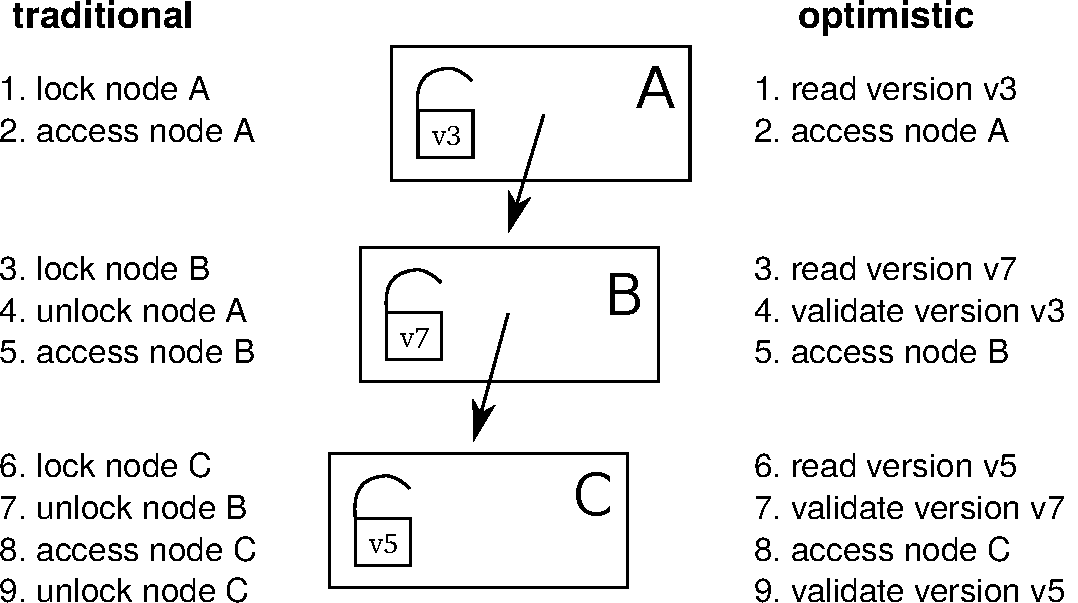
\includegraphics[width=0.65\linewidth]{olcall.pdf}
  \vspace{0.2cm}
  \caption{Comparison of a lookup operation in a 3-level tree using traditional lock coupling (left-hand side) vs.~optimistic lock coupling (right-hand side).}
  \label{fig:olc}
\end{figure}

The traditional and most common lock-based synchronization protocol for B-trees is lock coupling, which interleaves lock acquisitions while holding at most two locks at a time.
If, as we observed earlier, optimistic locks have similar semantics as traditional locks, it is natural to ask whether lock coupling can be combined with optimistic locks.
And indeed the answer is yes: One can almost mechanically translate traditional lock coupling code to optimistic lock coupling code.
This is illustrated in Figure~\ref{fig:olc}, which compares the traversal in a tree of height 3 using traditional and optimistic locks.
As the figure shows, the main difference is that locking is translated to reading the version and that unlocking becomes validation of the previously read version.
This simple change provides efficient lock-free tree traversal without the need to design a complex synchronization protocol.

It is important to emphasize the conceptual simplicity of OLC in comparison to data structures that use custom protocols like the Bw-tree~\cite{DBLP:conf/icde/LevandoskiLS13a}.
To implement lock-free access, the Bw-tree requires an indirection table, delta nodes, complex splitting and merging logic, retry logic, etc.
OLC, on the other hand, can directly be applied to B-trees mostly by adding the appropriate optimistic locking code and without modifying the node layout itself.
Therefore, OpenBw-Tree, an open source implementation of the Bw-tree, requires an order of magnitude more code than a B-tree based on OLC\footnote{Both implementations are available on GitHub: \url{https://github.com/wangziqi2016/index-microbench}}.
Given how difficult it is to develop, validate, and debug lock-free code, simplicity is obviously a major advantage.

\subsection{Correctness Aspects}

\begin{figure}
  % \centering
  %[basicstyle=\normalsize\ttfamily,showstringspaces=false,columns=fullflexible,breaklines=false,breakatwhitespace=true,numbers=none,numberstyle=\small,style=C,keepspaces=true]
\begin{lstlisting}[basicstyle=\ttfamily,language=C++,numbers=left,numberstyle=\small]
std::atomic<BTreeNode*> root;

// search for key in B+tree, returns payload in resultOut
bool lookup(Key key, Value& resultOut) {
   BTreeNode* node = root.load();
   uint64_t nodeVersion = node->readLockOrRestart();
   if (node != root.load()) // make sure the root is still the root
      restart();

   BTreeInner<Key>* parent = nullptr;
   uint64_t parentVersion = 0;

   while (node->isInner()) {
      auto inner = (BTreeInner*)node;

      // unlock parent and make current node the parent
      if (parent)
         parent->readUnlockOrRestart(parentVersion);
      parent = inner;
      parentVersion = nodeVersion;

      // search for next node
      node = inner->findChild(key);
      // validate 'inner' to ensure that 'node' pointer is valid
      inner->checkOrRestart(nodeVersion);
      // now it safe to dereference 'node' pointer (read its version)
      nodeVersion = node->readLockOrRestart();
   }

   // search in leaf and retrieve payload
   auto leaf = (BTreeLeaf*)node;
   bool success = leaf->findValue(key, resultOut);

   // unlock everything
   if (parent)
      parent->readUnlockOrRestart(parentVersion);
   node->readUnlockOrRestart(nodeVersion);

   return success;
}
\end{lstlisting}
  \vspace{0.2cm}
  \caption{B-tree lookup code using OLC. For simplicity, the restart logic is not shown.}
  \label{fig:lookup}
\end{figure}

So far, we have introduced the high-level ideas behind OLC and have stressed its similarity to traditional lock coupling.
Let us now discuss some cases where the close similarity between lock coupling and OLC breaks down.
To make this more concrete, we show the B-tree lookup code in Figure~\ref{fig:lookup}.
In the code, \texttt{readLockOrRestart} reads the lock version and \texttt{readUnlockOrRestart} validates that the read was correct.

One issue with OLC is that any pointer speculatively read from a node may point to invalid memory (if that node is modified concurrently).
Dereferencing such a pointer (e.g., to read its optimistic lock), may cause a segmentation fault or undefined behavior.
In the code shown in Figure~\ref{fig:lookup}, this problem is prevented by the extra check in line 25, which ensures that the read from the node containing the pointer was correct.
Without this additional validation, the code would in line 27 dereference the pointer speculatively read in line 23.
Note that the implementation of \texttt{checkOrRestart} is actually identical to \texttt{readUnlockOrRestart}.
We chose to give it a different name to highlight the fact that this extra check would not be necessary with read/write locks.

Another potential issue with optimistic locks is code that does not terminate.
Code that speculatively accesses a node, like an intra-node binary search, should be written in a way such that it always terminates---even in the presence of concurrent writes.
Otherwise, the validation code that detects the concurrent write will never run.
The binary search of a B-tree, for example, needs to be written in such a way that each comparison makes progress.
For some data structures that do not require loops in the traversal code (like ART) termination is trivially true.

\subsection{Implementation Details}

% implementation, efficiency
To implement an optimistic lock, one can combine the lock and the version counter into a single 64-bit\footnote{Even after subtracting one bit for the lock status, a back-of-the-envelope calculation can show that 63 bits are large enough to never overflow in practice.} word~\cite{artsync}.
A typical read operation will therefore merely consist of reading this version counter atomically.
In C++11 this can be implemented using the \texttt{std::atomic} type.

On x86, atomic reads are cheap because of x86's strong memory order guarantees.
No memory fences are required for sequentially-consistent loads, which are translated (by both GCC and clang) into standard \texttt{MOV} instructions.
Hence, the only effect of \texttt{std::atomic} for loads is preventing instruction re-ordering.
This makes version access and validation cheap.
Acquiring and releasing an optimistic lock in exclusive mode has comparable cost to a traditional lock:
A fairly expensive sequentially-consistent store is needed for acquiring a lock, while a standard \texttt{MOV} suffices for releasing it.
A simple sinlock-based implementation of optimistic locks can be found in the appendix of an earlier paper~\cite{artsync}.

OLC code must be able to handle restarts since validation or lock upgrade can fail due to concurrent writers.
Restarts can easily be implemented by wrapping the data structure operation in a loop (for simplicity not shown in Figure~\ref{fig:lookup}).
Such a loop also enables limiting the number of optimistic retry operations and falling back to pessimistic locking in cases of very heavy contention.
The ability to fall back to traditional locking is a major advantage of OLC in terms of robustness over lock-free approaches, which do not have this option.

In addition to the optimistic shared mode and the exclusive mode, optimistic locks also support a ``shared pessimistic'' mode, which physically acquires the lock in shared mode (allowing multiple concurrent readers but no writers).
This mode is useful for table (or range) scans that touch many tuples on a leaf page (which would otherwise easily abort).
Finally, let us mention that large range scans and table scans, should be broken up into several per-node traversals as is done in the LeanStore~\cite{leanstore} system.

Like all lock-free data structures, but unlike traditional locking and Hardware Transactional Memory~\cite{DBLP:conf/hpca/KarnagelDRLLSL14,DBLP:journals/pvldb/MakreshanskiLS15,htmtkde}, OLC requires care when deleting (and reusing) nodes.
The reason is that a deleting thread can never be sure that a node can be reclaimed because other threads might still be optimistically reading from that node.
Therefore, standard solutions like epoch-based reclamation~\cite{DBLP:conf/sosp/TuZKLM13}, hazard pointers~\cite{DBLP:journals/tpds/Michael04}, or optimized hazard pointers~\cite{DBLP:conf/spaa/BalmauGHZ16} need to be used.
These memory reclamation techniques are, however, largely orthogonal to the synchronization protocol itself.

%-lock-free is not a strong guarantee

\newpage
\section{Evaluation}\label{sec:evaluation}

Let us now experimentally evaluate the overhead and scalability of OLC.
For the experiments, we use an in-memory B+tree implemented in C++11 using templates, which is configured to use nodes of 4096 bytes, random 8 byte keys, and 8 byte payloads.
Based on this B-tree, we compare the following synchronization approaches:
\begin{itemize}
\item an OLC implementation\footnote{An almost identical OLC implementation is available on github: \url{https://github.com/wangziqi2016/index-microbench/tree/master/BTreeOLC}}
\item a variant based on traditional lock coupling and read/write locks
\item the unsynchronized B-tree, which obviously is only correct for read-only workloads but allows measuring the overhead of synchronization
\end{itemize}
Note that earlier work has compared the OLC implementation with a Bw-tree implementation~\cite{buzzword} and other state-of-the-art in-memory index structures.

We use a Haswell EP system with an Intel Xeon E5-2687W v3 CPU, which has 10 cores (20 ``Hyper-Threads'') and 25~MB of L3 cache.
The system is running Ubuntu 18.10 and we use GCC 8.2.0 to compile our code.
The CPU counters are obtained using the Linux perf API\footnote{We use the following convenience wrapper: \url{https://github.com/viktorleis/perfevent}}.

\begin{table}
  \caption{Performance and CPU counters for lookup and insert operations in a B-tree with 100M keys. We perform 100M operations and normalize the CPU counters by that number.}
  \label{tab:overhead}
  \centering
  \begin{tabular}{lrrrrrrr}\toprule
                    &         &        &        & instruc-  & L1     & L3     & branch \\
                    & threads & M op/s & cycles & tions & misses & misses & misses \\\midrule
lookup (no sync.)   & 1       & 1.72   & 2028   & 283     & 39.1   & 14.9   & 16.1   \\
lookup (OLC)        & 1       & 1.65   & 2107   & 370     & 43.9   & 15.1   & 16.7   \\
lookup (lock coup.) & 1       & 1.72   & 2078   & 365     & 42.3   & 16.9   & 15.7   \\\midrule
insert (no sync.)   & 1       & 1.51   & 2286   & 530     & 59.8   & 31.1   & 17.3   \\
insert (OLC)        & 1       & 1.50   & 2303   & 629     & 61.2   & 31.1   & 16.5   \\
insert (lock coup.) & 1       & 1.41   & 2473   & 644     & 61.0   & 31.0   & 17.2   \\\midrule
lookup (no sync.)   & 10      & 15.48  & 2058   & 283     & 38.6   & 15.5   & 16.0   \\
lookup (OLC)        & 10      & 14.60  & 2187   & 370     & 43.8   & 15.8   & 16.8   \\
lookup (lock coup.) & 10      & 5.71   & 5591   & 379     & 54.2   & 17.0   & 14.8   \\\midrule
insert (no sync.)   & 10      & -      & -      & -       & -      & -      & -      \\
insert (OLC)        & 10      & 10.46  & 2940   & 656     & 62.0   & 32.5   & 16.8   \\
insert (lock coup.) & 10      & 7.55   & 4161   & 667     & 75.0   & 28.6   & 16.2   \\
    \bottomrule
\end{tabular}
\end{table}

Table~\ref{tab:overhead} compares the performance and CPU counters for lookup and insert operations in a B-tree with 100M keys.
With {\em single-threaded} execution, we observe that all three approaches have very similar performance.
Adding traditional or optimistic locks to unsynchronized B-tree code results in up to 30\% of additional instructions without affecting single-threaded performance much.

\begin{figure}
  \centering
  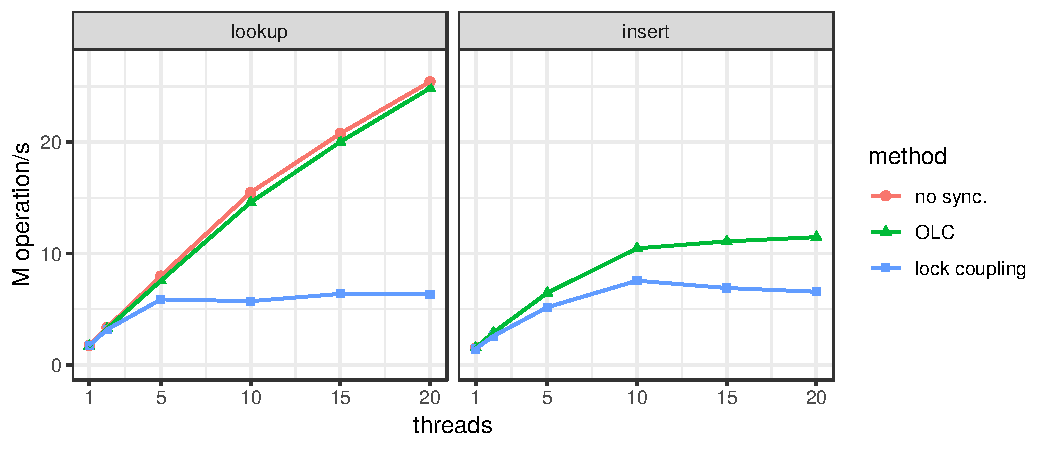
\includegraphics[width=\linewidth]{scale.pdf}
  \vspace{0.2cm}
  \caption{Scalability on 10-core system for B-tree operations (100M values).}
  \label{fig:scale}
\end{figure}

As Figure~\ref{fig:scale} shows, the results change dramatically once we use multiple threads.
For lookup, the scalability of OLC is near-linear up to 20 threads, even though the system has only 10 ``real cores''.
The OLC scalability for insert is also respectable (though not quite as linear because multi-threaded insertion approaches the memory bandwidth of our processor).
The figure also shows that the results of traditional lock coupling with read/write locks are significantly worse than OLC.
With 20 threads, lookup with OLC is 3.9$\times$ faster than traditional lock coupling.

\section{Summary}\label{sec:conc}

Optimistic Lock Coupling (OLC) is an effective synchronization method that combines the simplicity of traditional lock coupling with the superior scalability of lock-free approaches.
OLC is widely applicable and has already been successfully used to synchronize several data structures, including B-trees, binary search trees, and different trie variants.
These features make it highly attractive for modern database systems as well as performance-critical systems software in general.

\begin{thebibliography}{10}

\bibitem{DBLP:conf/spaa/BalmauGHZ16}
O.~Balmau, R.~Guerraoui, M.~Herlihy, and I.~Zablotchi.
\newblock Fast and robust memory reclamation for concurrent data structures.
\newblock In {\em SPAA}, 2016.

\bibitem{DBLP:journals/acta/BayerS77}
R.~Bayer and M.~Schkolnick.
\newblock Concurrency of operations on {B}-trees.
\newblock {\em Acta Informatica}, 9, 1977.

\bibitem{hot}
R.~Binna, E.~Zangerle, M.~Pichl, G.~Specht, and V.~Leis.
\newblock {HOT}: A height optimized trie index for main-memory database
  systems.
\newblock In {\em SIGMOD}, 2018.

\bibitem{DBLP:conf/ppopp/BronsonCCO10}
N.~G. Bronson, J.~Casper, H.~Chafi, and K.~Olukotun.
\newblock A practical concurrent binary search tree.
\newblock In {\em PPOPP}, 2010.

\bibitem{DBLP:conf/vldb/ChaHKK01}
S.~K. Cha, S.~Hwang, K.~Kim, and K.~Kwon.
\newblock Cache-conscious concurrency control of main-memory indexes on
  shared-memory multiprocessor systems.
\newblock In {\em VLDB}, 2001.

\bibitem{intel}
I.~Cutress.
\newblock {Intel} goes for 48-cores: {Cascade-AP} with multi-chip package
  coming soon.
\newblock
  \url{https://www.anandtech.com/show/13535/intel-goes-for-48cores-cascade-ap},
  2018 (accessed January, 2019).

\bibitem{DBLP:conf/cidr/FaleiroA17}
J.~M. Faleiro and D.~J. Abadi.
\newblock Latch-free synchronization in database systems: Silver bullet or
  fool's gold?
\newblock In {\em CIDR}, 2017.

\bibitem{DBLP:journals/ftdb/Graefe11}
G.~Graefe.
\newblock Modern {B}-tree techniques.
\newblock {\em Foundations and Trends in Databases}, 3(4), 2011.

\bibitem{DBLP:conf/hpca/KarnagelDRLLSL14}
T.~Karnagel, R.~Dementiev, R.~Rajwar, K.~Lai, T.~Legler, B.~Schlegel, and
  W.~Lehner.
\newblock Improving in-memory database index performance with
  {Intel}\({}^{\mbox{{\textregistered}}}\) transactional synchronization
  extensions.
\newblock In {\em HPCA}, 2014.

\bibitem{DBLP:journals/tods/LehmanY81}
P.~L. Lehman and S.~B. Yao.
\newblock Efficient locking for concurrent operations on {B}-trees.
\newblock {\em {ACM} Trans. Database Syst.}, 6(4), 1981.

\bibitem{leanstore}
V.~Leis, M.~Haubenschild, A.~Kemper, and T.~Neumann.
\newblock Leanstore: In-memory data management beyond main memory.
\newblock In {\em ICDE}, 2018.

\bibitem{art}
V.~Leis, A.~Kemper, and T.~Neumann.
\newblock The adaptive radix tree: {ARTful} indexing for main-memory databases.
\newblock In {\em ICDE}, 2013.

\bibitem{htmtkde}
V.~Leis, A.~Kemper, and T.~Neumann.
\newblock Scaling {HTM}-supported database transactions to many cores.
\newblock {\em {IEEE} Trans. Knowl. Data Eng.}, 28(2), 2016.

\bibitem{artsync}
V.~Leis, F.~Scheibner, A.~Kemper, and T.~Neumann.
\newblock The {ART} of practical synchronization.
\newblock In {\em DaMoN}, 2016.

\bibitem{DBLP:conf/icde/LevandoskiLS13a}
J.~J. Levandoski, D.~B. Lomet, and S.~Sengupta.
\newblock The {Bw}-tree: A {B}-tree for new hardware platforms.
\newblock In {\em ICDE}, 2013.

\bibitem{DBLP:journals/pvldb/MakreshanskiLS15}
D.~Makreshanski, J.~J. Levandoski, and R.~Stutsman.
\newblock To lock, swap, or elide: On the interplay of hardware transactional
  memory and lock-free indexing.
\newblock {\em {PVLDB}}, 8(11), 2015.

\bibitem{DBLP:dblp_conf/eurosys/MaoKM12}
Y.~Mao, E.~Kohler, and R.~T. Morris.
\newblock Cache craftiness for fast multicore key-value storage.
\newblock In {\em EuroSys}, 2012.

\bibitem{DBLP:journals/tpds/Michael04}
M.~M. Michael.
\newblock Hazard pointers: Safe memory reclamation for lock-free objects.
\newblock {\em {IEEE} Trans. Parallel Distrib. Syst.}, 15(6), 2004.

\bibitem{DBLP:journals/jacm/ShalevS06}
O.~Shalev and N.~Shavit.
\newblock Split-ordered lists: Lock-free extensible hash tables.
\newblock {\em J. {ACM}}, 53(3), 2006.

\bibitem{amd}
A.~Shilov.
\newblock {AMD} previews {EPYC} ‘{Rome}’ processor: Up to 64 {Zen} 2 cores.
\newblock
  \url{https://www.anandtech.com/show/13561/amd-previews-epyc-rome-processor-up-to-64-zen-2-cores},
  2018 (accessed January, 2019).

\bibitem{DBLP:conf/sosp/TuZKLM13}
S.~Tu, W.~Zheng, E.~Kohler, B.~Liskov, and S.~Madden.
\newblock Speedy transactions in multicore in-memory databases.
\newblock In {\em SOSP}, 2013.

\bibitem{buzzword}
Z.~Wang, A.~Pavlo, H.~Lim, V.~Leis, H.~Zhang, M.~Kaminsky, and D.~Andersen.
\newblock Building a {Bw}-tree takes more than just buzz words.
\newblock In {\em SIGMOD}, 2018.

\end{thebibliography}


%\bibliographystyle{abbrv}
%\bibliography{main}

\end{document}

\end{article}
\begin{article}
{Approximate Nearest Neighbor Search in High Dimensional Vector Databases: Current Research and Future Directions}
{Yao Tian, Ziyang Yue, Ruiyuan Zhang, Xi Zhao, Bolong Zhen, Xiaofang Zhou}
\pdfminorversion=5
\documentclass[11pt]{article}
\usepackage{deauthor,times,graphicx,caption,microtype}
\usepackage{hyperref}
\usepackage{listings}
\usepackage{booktabs}

\begin{document}

\title{Optimistic Lock Coupling: A Scalable and Efficient General-Purpose Synchronization Method}

\author{Viktor Leis, Michael Haubenschild\raisebox{0.9ex}{$\ast$}, Thomas Neumann\\ Technische Universit{\"a}t M{\"u}nchen \hspace{0.7cm} Tableau Software\raisebox{0.9ex}{$\ast$} \\ {\{leis,neumann\}{@}in.tum.de} \hspace{0.7cm} {mhaubenschild{@}tableau.com\raisebox{0.9ex}{$\ast$}}}

\maketitle

\begin{abstract}
As the number of cores on commodity processors continues to increase, scalability becomes more and more crucial for overall performance.
Scalable and efficient concurrent data structures are particularly important, as these are often the building blocks of parallel algorithms.
Unfortunately, traditional synchronization techniques based on fine-grained locking have been shown to be unscalable on modern multi-core CPUs.
Lock-free data structures, on the other hand, are extremely difficult to design and often incur significant overhead.

In this work, we make the case for Optimistic Lock Coupling as a practical alternative to both traditional locking and the lock-free approach.
We show that Optimistic Lock Coupling is highly scalable and almost as simple to implement as traditional lock coupling.
Another important advantage is that it is easily applicable to most tree-like data structures.
We therefore argue that Optimistic Lock Coupling, rather than a complex and error-prone custom synchronization protocol, should be the default choice for performance-critical data structures.
\end{abstract}

\section{Introduction}

% more and more cores
Today, Intel's commodity server processors have up to 28 cores and its upcoming microarchitecture will have up to 48 cores per socket~\cite{intel}.
Similarly, AMD currently stands at 32 cores and this number is expected to double in the next generation~\cite{amd}.
Since both platforms support simultaneous multithreading (also known as hyperthreading), affordable commodity servers (with up to two sockets) will soon routinely have between 100 and 200 hardware threads.

% data structure scalability is important
With such a high degree of hardware parallelism, efficient data processing crucially depends on how well concurrent data structures scale.
Internally, database systems use a plethora of data structures like table heaps, internal work queues, and, most importantly, index structures.
Any of these can easily become a scalability (and therefore overall performance) bottleneck on many-core CPUs.

% traditional synchronization: fine-grained locks, slow, cache invalidation
Traditionally, database systems synchronize internal data structures using fine-grained reader/writer locks\footnote{In this work, we focus on data structure synchronization rather than high-level transaction semantics and therefore use the term {\em lock} for what would typically be called {\em latch} in the database literature. We thus follow common computer science (rather than database) terminology.}.
Unfortunately, while fine-grained locking makes lock contention unlikely, it still results in bad scalability because lock acquisition and release require writing to shared memory.
Due to the way cache coherency is implemented on modern multi-core CPUs, these writes cause additional cache misses\footnote{The cache coherency protocol ensures that all copies of a cache line on other cores are invalidated before the write can proceed.} and the cache line containing the lock's internal data becomes a point of physical contention.
As a result, any frequently-accessed lock (e.g., the lock of the root node of a B-tree) severely limits scalability.

% lock-free bw-tree: no more latches, but indirections, extremely complex
Lock-free data structures like the Bw-tree~\cite{DBLP:conf/icde/LevandoskiLS13a} (a lock-free B-tree variant) or the Split-Ordered List~\cite{DBLP:journals/jacm/ShalevS06} (a lock-free hash table) do not acquire any locks and therefore generally scale much better than locking-based approaches (in particular for read-mostly workloads).
However, lock-free synchronization has other downsides:
First, it is very difficult and results in extremely complex and error-prone code (when compared to locking).
Second, because the functionality of atomic primitives provided by the hardware (e.g., atomically compare-and-swap 8 bytes) is limited, complex operations require additional indirections within the data structure.
For example, the Bw-tree requires an indirection table and the Split-Ordered List requires ``dummy nodes'', resulting in overhead due to additional cache misses.

% OLC for the win
In this paper we make the case for {\em Optimistic Lock Coupling (OLC)}, a synchronization method that combines some of the best properties of lock-based and lock-free synchronization.
OLC utilizes a special lock type that can be used in two modes:
The first mode is similar to a traditional mutex and excludes other threads by physically acquiring the underlying lock.
In the second mode, reads can proceed optimistically by validating a version counter that is embedded in the lock (similar to optimistic concurrency control).
The first mode is typically used by writers and the second mode by readers.
Besides this special lock type, OLC is based on the observation that optimistic lock validations can be interleaved/coupled---similar to the pair-wise interleaved lock acquisition of traditional lock coupling.
Hence, the name Optimistic Lock Coupling.

OLC has a number of desirable features:
\begin{itemize}
\item By reducing the number of writes to shared memory locations and thereby avoiding cache invalidations, it {\bf scales well} for most workloads.
\item In comparison to unsynchronized code, it requires few additional CPU instructions making it {\bf efficient}.
\item OLC is {\bf widely applicable} to different data structures. It has already been successfully used for synchronizing binary search trees~\cite{DBLP:conf/ppopp/BronsonCCO10}, tries~\cite{artsync}, trie/B-tree hybrids~\cite{DBLP:dblp_conf/eurosys/MaoKM12}, and B-trees~\cite{buzzword}.
\item In comparison to the lock-free paradigm, it is also {\bf easy to use} and requires few modifications to existing, single-threaded data structures.
\end{itemize}
Despite these positive features and its simplicity, OLC is not yet widely known.
The goal of this paper is therefore to popularize this simple idea and to make a case for it.
We argue that OLC deserves to be widely known.
It is a good default synchronization paradigm---more complex, data structure-specific protocols are seldom beneficial.

The rest of the paper is organized as follows.
Section~\ref{sec:related} discusses related work, tracing the history of OLC and its underlying ideas in the literature.
The core of the paper is Section~\ref{sec:olc}, which describes the ideas behind OLC and how it can be used to synchronize complex data structures.
In Section~\ref{sec:evaluation} we experimentally show that OLC has low overhead and scales well when used to synchronize an in-memory B-tree.
We summarize the paper in Section~\ref{sec:conc}.

\newpage
\section{Related Work}\label{sec:related}

Lock coupling has been proposed as a method for allowing concurrent operations on B-trees in 1977~\cite{DBLP:journals/acta/BayerS77}.
This traditional and still widely-used method, described in detail in Graefe's B-tree survey~\cite{DBLP:journals/ftdb/Graefe11}, is also called ``latch coupling'', ``hand-over-hand locking'', and ``crabbing''.
Because at most two locks are held at-a-time during tree traversal, this technique seemingly allows for a high degree of parallelism---in particular if read/write locks are used to enable inner nodes to be locked in shared mode.
However, as we show in Section~\ref{sec:evaluation}, on modern hardware lock acquisition (even in shared mode) results in suboptimal scalability.

An early alternative from 1981 is a B-tree variant called B-link tree~\cite{DBLP:journals/tods/LehmanY81}, which only holds a single lock at a time.
It is based on the observation that between the release of the parent lock and the acquisition of the child lock, the only ``dangerous'' thing that could have happened is the split of a child node (assuming one does not implement merge operations).
Thus, when a split happens, the key being searched might end up on a neighboring node to the right of the current child node.
A B-link tree traversal therefore detects this condition and, if needed, transparently proceeds to the neighboring node.
Releasing the parent lock early is highly beneficial when the child node needs to be fetched from disk.
For in-memory workloads, however, the B-link tree has the same scalability issues as lock coupling (it acquires just as many locks).

The next major advance, Optimistic Latch-Free Index Traversal (OLFIT)~\cite{DBLP:conf/vldb/ChaHKK01}, was proposed in 2001.
OLFIT introduced the idea of a combined lock/update counter, which we call {\em optimistic lock}. % , for lack of a better name,
Based on these per-node optimistic locks and the synchronization protocol of the B-link tree, OLFIT finally achieves good scalability on parallel processors.
The OLFIT protocol is fairly complex, as it requires both the non-trivial B-link protocol and optimistic locks.
Furthermore, like the B-link tree protocol, it does not support merging nodes, and is specific to B-trees (cannot easily be applied to other data structures).

In the following two decades, the growth of main-memory capacity led to much research into other data structures besides the venerable B-tree.
Particularly relevant for our discussion is Bronson et al.'s~\cite{DBLP:conf/ppopp/BronsonCCO10} concurrent binary search tree, which is based on optimistic version validation and has a sophisticated, data structure-specific synchronization protocol.
To the best of our knowledge, this 2010 paper is the first that, as part of its protocol, interleaves version validation across nodes---rather than validating each node separately like OLFIT.
In that paper, this idea is called ``hand-over-hand, optimistic validation'', while we prefer the term Optimistic Lock Coupling to highlight the close resemblance to traditional lock coupling.
Similarly, Mao et al.'s~\cite{DBLP:dblp_conf/eurosys/MaoKM12} Masstree (a concurrent hybrid trie/B-tree) is also based on the same ideas, but again uses them as part of a more complex protocol.

The Adaptive Radix Tree (ART)~\cite{art} is another recent in-memory data structure, which we proposed in 2013.
In contrast to the two data structures just mentioned, it was originally designed with single-threaded performance in mind without supporting concurrency.
To add support for concurrency, we initially started designing a custom protocol called Read-Optimized Write Exclusion (ROWEX)~\cite{artsync}, which turned out to be non-trivial and requires modifications of the underlying data structure\footnote{Note that ROWEX is already easier to apply to existing data structures than the lock-free approach. The difficulty depends on the data structure. Applying ROWEX is hard for B-trees with sorted keys and fairly easy for copy-on-write data structures like the Height Optimized Trie~\cite{hot}---with ART being somewhere in the middle.}.
However, fairly late in the project, we also realized, that OLC {\em alone} (rather than as part of a more complex protocol) is sufficient to synchronize ART.
No other changes to the data structure were necessary.
Both approaches were published and experimentally evaluated in a followup paper~\cite{artsync}, which shows that, despite its simplicity, OLC is efficient, scalable, and generally outperforms ROWEX.

Similar results were recently published regarding B-trees~\cite{buzzword}.
In this experimental study a simple OLC-based synchronization outperformed the Bw-tree~\cite{DBLP:conf/icde/LevandoskiLS13a}, a complex lock-free synchronization approach.
Another recent paper shows that for write-intensive workloads, locking often performs better than lock-free synchronization~\cite{DBLP:conf/cidr/FaleiroA17}.
These experiences indicate that OLC is a general-purpose synchronization paradigm and motivate the current paper.

%foster b-tree\cite{DBLP:journals/tods/GraefeKK12}
%Shasha theory~\cite{DBLP:journals/tods/ShashaG88}

\section{Optimistic Lock Coupling}\label{sec:olc}

% locks suck
The standard technique for inter-thread synchronization is mutual exclusion using fine-grained locks.
In a B-tree, for example, every node usually has its own associated lock, which is acquired before accessing that node.
The problem of locking on modern multi- and many-core processors is that lock acquisition and release require writing to the shared memory location that implements the lock.
This write causes exclusive ownership of the underlying cache line and invalidates copies of it on all other processor cores.
For hierarchical, tree-like data structures, the lock of the root node becomes a point of physical contention---even in read-only workloads and even when read/write locks are used.
Depending on the specific data structure, number of cores, cache coherency protocol implementation, cache topology, whether Non-Uniform Memory Access (NUMA) is used, locking can even result in multi-threaded performance that is worse than single-threaded execution.

% in b-trees this happens very much
The inherent pessimism of locking is particularly unfortunate for B-trees:
Despite the fact that logical modifications of the root node are very infrequent, every B-tree operation must lock the root node during tree traversal\footnote{To a lesser extent this obviously applies to all inner nodes, not just the root.}.
Even the vast majority of update operations (with the exception of splits and merges), only modify a single leaf node.
These observations indicate that a more optimistic approach, which does not require locking inner nodes, would be very beneficial for B-trees.

\subsection{Optimistic Locks}

% optimism to the rescue
As the name indicates, optimistic locks try to solve the scalability issues of traditional locks using an optimistic approach.
Instead of always physically acquiring locks, even for nodes that are unlikely to be modified simultaneously, after-the-fact validation is used to detect conflicts.
This is done by augmenting each lock with a version/update counter that is incremented on every modification.
Using this version counter, readers can optimistically proceed before validating that the version did not change to ensure that the read was safe.
If validation fails, the operation is restarted.

% details on opt locks
Using optimistic locks, a read-only node access (i.e., the majority of all operations in a B-tree) does not acquire the lock and does not increment the version counter.
Instead, it performs the following steps:
\begin{enumerate}
\item read lock version (restart if lock is not free)
\item access node
\item read the version again and validate that it has not changed in the meantime
\end{enumerate}
If the last step (the validation) fails, the operation has to be restarted.
Write operations, on the other hand, are more similar to traditional locking:
\begin{enumerate}
\item acquire lock (wait if necessary)
\item access/write to node
\item increment version and unlock node
\end{enumerate}
Writes can therefore protect a node from other writes.

% similar to locks
As we observed in an earlier paper~\cite{artsync}, because of similar semantics, optimistic locks can be hidden behind an API very similar to traditional read/write locks.
Both approaches have an exclusive lock mode, and acquiring a traditional lock in shared mode is analogous to optimistic version validation.
Furthermore, like with some implementations of traditional read/write locks, optimistic locks allow upgrading a shared lock to an exclusive lock.
Lock upgrades are, for example, used to avoid most B-tree update operations from having to lock inner nodes.
In our experience, the close resemblance of optimistic and traditional locks simplifies the reasoning about optimistic locks;
one can apply similar thinking as in traditional lock-based protocols.

\subsection{Lock Coupling with Optimistic Locks}

\begin{figure}
  \centering
  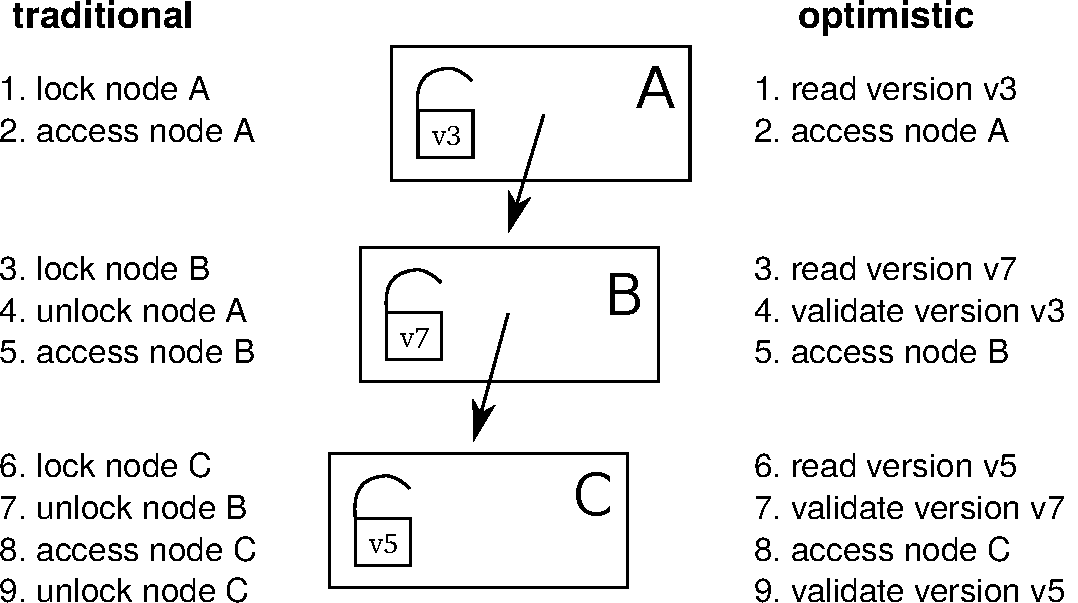
\includegraphics[width=0.65\linewidth]{olcall.pdf}
  \vspace{0.2cm}
  \caption{Comparison of a lookup operation in a 3-level tree using traditional lock coupling (left-hand side) vs.~optimistic lock coupling (right-hand side).}
  \label{fig:olc}
\end{figure}

The traditional and most common lock-based synchronization protocol for B-trees is lock coupling, which interleaves lock acquisitions while holding at most two locks at a time.
If, as we observed earlier, optimistic locks have similar semantics as traditional locks, it is natural to ask whether lock coupling can be combined with optimistic locks.
And indeed the answer is yes: One can almost mechanically translate traditional lock coupling code to optimistic lock coupling code.
This is illustrated in Figure~\ref{fig:olc}, which compares the traversal in a tree of height 3 using traditional and optimistic locks.
As the figure shows, the main difference is that locking is translated to reading the version and that unlocking becomes validation of the previously read version.
This simple change provides efficient lock-free tree traversal without the need to design a complex synchronization protocol.

It is important to emphasize the conceptual simplicity of OLC in comparison to data structures that use custom protocols like the Bw-tree~\cite{DBLP:conf/icde/LevandoskiLS13a}.
To implement lock-free access, the Bw-tree requires an indirection table, delta nodes, complex splitting and merging logic, retry logic, etc.
OLC, on the other hand, can directly be applied to B-trees mostly by adding the appropriate optimistic locking code and without modifying the node layout itself.
Therefore, OpenBw-Tree, an open source implementation of the Bw-tree, requires an order of magnitude more code than a B-tree based on OLC\footnote{Both implementations are available on GitHub: \url{https://github.com/wangziqi2016/index-microbench}}.
Given how difficult it is to develop, validate, and debug lock-free code, simplicity is obviously a major advantage.

\subsection{Correctness Aspects}

\begin{figure}
  % \centering
  %[basicstyle=\normalsize\ttfamily,showstringspaces=false,columns=fullflexible,breaklines=false,breakatwhitespace=true,numbers=none,numberstyle=\small,style=C,keepspaces=true]
\begin{lstlisting}[basicstyle=\ttfamily,language=C++,numbers=left,numberstyle=\small]
std::atomic<BTreeNode*> root;

// search for key in B+tree, returns payload in resultOut
bool lookup(Key key, Value& resultOut) {
   BTreeNode* node = root.load();
   uint64_t nodeVersion = node->readLockOrRestart();
   if (node != root.load()) // make sure the root is still the root
      restart();

   BTreeInner<Key>* parent = nullptr;
   uint64_t parentVersion = 0;

   while (node->isInner()) {
      auto inner = (BTreeInner*)node;

      // unlock parent and make current node the parent
      if (parent)
         parent->readUnlockOrRestart(parentVersion);
      parent = inner;
      parentVersion = nodeVersion;

      // search for next node
      node = inner->findChild(key);
      // validate 'inner' to ensure that 'node' pointer is valid
      inner->checkOrRestart(nodeVersion);
      // now it safe to dereference 'node' pointer (read its version)
      nodeVersion = node->readLockOrRestart();
   }

   // search in leaf and retrieve payload
   auto leaf = (BTreeLeaf*)node;
   bool success = leaf->findValue(key, resultOut);

   // unlock everything
   if (parent)
      parent->readUnlockOrRestart(parentVersion);
   node->readUnlockOrRestart(nodeVersion);

   return success;
}
\end{lstlisting}
  \vspace{0.2cm}
  \caption{B-tree lookup code using OLC. For simplicity, the restart logic is not shown.}
  \label{fig:lookup}
\end{figure}

So far, we have introduced the high-level ideas behind OLC and have stressed its similarity to traditional lock coupling.
Let us now discuss some cases where the close similarity between lock coupling and OLC breaks down.
To make this more concrete, we show the B-tree lookup code in Figure~\ref{fig:lookup}.
In the code, \texttt{readLockOrRestart} reads the lock version and \texttt{readUnlockOrRestart} validates that the read was correct.

One issue with OLC is that any pointer speculatively read from a node may point to invalid memory (if that node is modified concurrently).
Dereferencing such a pointer (e.g., to read its optimistic lock), may cause a segmentation fault or undefined behavior.
In the code shown in Figure~\ref{fig:lookup}, this problem is prevented by the extra check in line 25, which ensures that the read from the node containing the pointer was correct.
Without this additional validation, the code would in line 27 dereference the pointer speculatively read in line 23.
Note that the implementation of \texttt{checkOrRestart} is actually identical to \texttt{readUnlockOrRestart}.
We chose to give it a different name to highlight the fact that this extra check would not be necessary with read/write locks.

Another potential issue with optimistic locks is code that does not terminate.
Code that speculatively accesses a node, like an intra-node binary search, should be written in a way such that it always terminates---even in the presence of concurrent writes.
Otherwise, the validation code that detects the concurrent write will never run.
The binary search of a B-tree, for example, needs to be written in such a way that each comparison makes progress.
For some data structures that do not require loops in the traversal code (like ART) termination is trivially true.

\subsection{Implementation Details}

% implementation, efficiency
To implement an optimistic lock, one can combine the lock and the version counter into a single 64-bit\footnote{Even after subtracting one bit for the lock status, a back-of-the-envelope calculation can show that 63 bits are large enough to never overflow in practice.} word~\cite{artsync}.
A typical read operation will therefore merely consist of reading this version counter atomically.
In C++11 this can be implemented using the \texttt{std::atomic} type.

On x86, atomic reads are cheap because of x86's strong memory order guarantees.
No memory fences are required for sequentially-consistent loads, which are translated (by both GCC and clang) into standard \texttt{MOV} instructions.
Hence, the only effect of \texttt{std::atomic} for loads is preventing instruction re-ordering.
This makes version access and validation cheap.
Acquiring and releasing an optimistic lock in exclusive mode has comparable cost to a traditional lock:
A fairly expensive sequentially-consistent store is needed for acquiring a lock, while a standard \texttt{MOV} suffices for releasing it.
A simple sinlock-based implementation of optimistic locks can be found in the appendix of an earlier paper~\cite{artsync}.

OLC code must be able to handle restarts since validation or lock upgrade can fail due to concurrent writers.
Restarts can easily be implemented by wrapping the data structure operation in a loop (for simplicity not shown in Figure~\ref{fig:lookup}).
Such a loop also enables limiting the number of optimistic retry operations and falling back to pessimistic locking in cases of very heavy contention.
The ability to fall back to traditional locking is a major advantage of OLC in terms of robustness over lock-free approaches, which do not have this option.

In addition to the optimistic shared mode and the exclusive mode, optimistic locks also support a ``shared pessimistic'' mode, which physically acquires the lock in shared mode (allowing multiple concurrent readers but no writers).
This mode is useful for table (or range) scans that touch many tuples on a leaf page (which would otherwise easily abort).
Finally, let us mention that large range scans and table scans, should be broken up into several per-node traversals as is done in the LeanStore~\cite{leanstore} system.

Like all lock-free data structures, but unlike traditional locking and Hardware Transactional Memory~\cite{DBLP:conf/hpca/KarnagelDRLLSL14,DBLP:journals/pvldb/MakreshanskiLS15,htmtkde}, OLC requires care when deleting (and reusing) nodes.
The reason is that a deleting thread can never be sure that a node can be reclaimed because other threads might still be optimistically reading from that node.
Therefore, standard solutions like epoch-based reclamation~\cite{DBLP:conf/sosp/TuZKLM13}, hazard pointers~\cite{DBLP:journals/tpds/Michael04}, or optimized hazard pointers~\cite{DBLP:conf/spaa/BalmauGHZ16} need to be used.
These memory reclamation techniques are, however, largely orthogonal to the synchronization protocol itself.

%-lock-free is not a strong guarantee

\newpage
\section{Evaluation}\label{sec:evaluation}

Let us now experimentally evaluate the overhead and scalability of OLC.
For the experiments, we use an in-memory B+tree implemented in C++11 using templates, which is configured to use nodes of 4096 bytes, random 8 byte keys, and 8 byte payloads.
Based on this B-tree, we compare the following synchronization approaches:
\begin{itemize}
\item an OLC implementation\footnote{An almost identical OLC implementation is available on github: \url{https://github.com/wangziqi2016/index-microbench/tree/master/BTreeOLC}}
\item a variant based on traditional lock coupling and read/write locks
\item the unsynchronized B-tree, which obviously is only correct for read-only workloads but allows measuring the overhead of synchronization
\end{itemize}
Note that earlier work has compared the OLC implementation with a Bw-tree implementation~\cite{buzzword} and other state-of-the-art in-memory index structures.

We use a Haswell EP system with an Intel Xeon E5-2687W v3 CPU, which has 10 cores (20 ``Hyper-Threads'') and 25~MB of L3 cache.
The system is running Ubuntu 18.10 and we use GCC 8.2.0 to compile our code.
The CPU counters are obtained using the Linux perf API\footnote{We use the following convenience wrapper: \url{https://github.com/viktorleis/perfevent}}.

\begin{table}
  \caption{Performance and CPU counters for lookup and insert operations in a B-tree with 100M keys. We perform 100M operations and normalize the CPU counters by that number.}
  \label{tab:overhead}
  \centering
  \begin{tabular}{lrrrrrrr}\toprule
                    &         &        &        & instruc-  & L1     & L3     & branch \\
                    & threads & M op/s & cycles & tions & misses & misses & misses \\\midrule
lookup (no sync.)   & 1       & 1.72   & 2028   & 283     & 39.1   & 14.9   & 16.1   \\
lookup (OLC)        & 1       & 1.65   & 2107   & 370     & 43.9   & 15.1   & 16.7   \\
lookup (lock coup.) & 1       & 1.72   & 2078   & 365     & 42.3   & 16.9   & 15.7   \\\midrule
insert (no sync.)   & 1       & 1.51   & 2286   & 530     & 59.8   & 31.1   & 17.3   \\
insert (OLC)        & 1       & 1.50   & 2303   & 629     & 61.2   & 31.1   & 16.5   \\
insert (lock coup.) & 1       & 1.41   & 2473   & 644     & 61.0   & 31.0   & 17.2   \\\midrule
lookup (no sync.)   & 10      & 15.48  & 2058   & 283     & 38.6   & 15.5   & 16.0   \\
lookup (OLC)        & 10      & 14.60  & 2187   & 370     & 43.8   & 15.8   & 16.8   \\
lookup (lock coup.) & 10      & 5.71   & 5591   & 379     & 54.2   & 17.0   & 14.8   \\\midrule
insert (no sync.)   & 10      & -      & -      & -       & -      & -      & -      \\
insert (OLC)        & 10      & 10.46  & 2940   & 656     & 62.0   & 32.5   & 16.8   \\
insert (lock coup.) & 10      & 7.55   & 4161   & 667     & 75.0   & 28.6   & 16.2   \\
    \bottomrule
\end{tabular}
\end{table}

Table~\ref{tab:overhead} compares the performance and CPU counters for lookup and insert operations in a B-tree with 100M keys.
With {\em single-threaded} execution, we observe that all three approaches have very similar performance.
Adding traditional or optimistic locks to unsynchronized B-tree code results in up to 30\% of additional instructions without affecting single-threaded performance much.

\begin{figure}
  \centering
  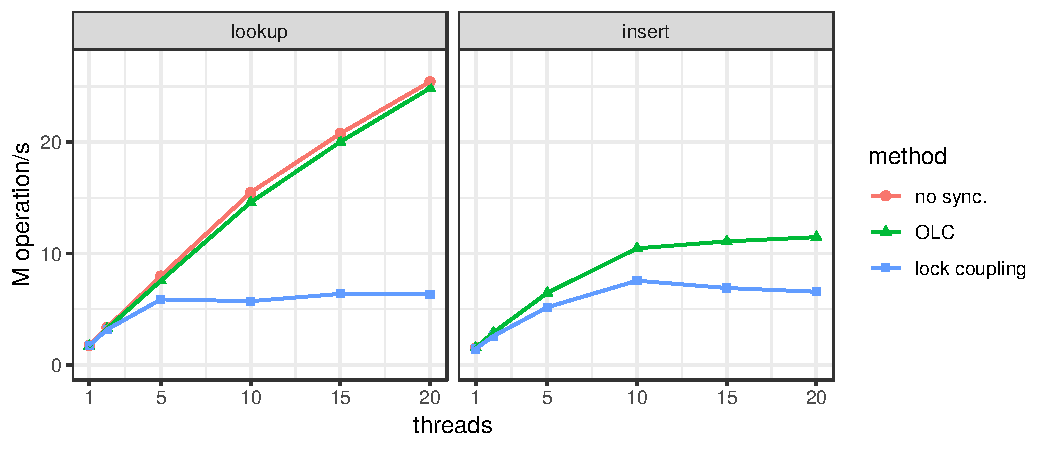
\includegraphics[width=\linewidth]{scale.pdf}
  \vspace{0.2cm}
  \caption{Scalability on 10-core system for B-tree operations (100M values).}
  \label{fig:scale}
\end{figure}

As Figure~\ref{fig:scale} shows, the results change dramatically once we use multiple threads.
For lookup, the scalability of OLC is near-linear up to 20 threads, even though the system has only 10 ``real cores''.
The OLC scalability for insert is also respectable (though not quite as linear because multi-threaded insertion approaches the memory bandwidth of our processor).
The figure also shows that the results of traditional lock coupling with read/write locks are significantly worse than OLC.
With 20 threads, lookup with OLC is 3.9$\times$ faster than traditional lock coupling.

\section{Summary}\label{sec:conc}

Optimistic Lock Coupling (OLC) is an effective synchronization method that combines the simplicity of traditional lock coupling with the superior scalability of lock-free approaches.
OLC is widely applicable and has already been successfully used to synchronize several data structures, including B-trees, binary search trees, and different trie variants.
These features make it highly attractive for modern database systems as well as performance-critical systems software in general.

\begin{thebibliography}{10}

\bibitem{DBLP:conf/spaa/BalmauGHZ16}
O.~Balmau, R.~Guerraoui, M.~Herlihy, and I.~Zablotchi.
\newblock Fast and robust memory reclamation for concurrent data structures.
\newblock In {\em SPAA}, 2016.

\bibitem{DBLP:journals/acta/BayerS77}
R.~Bayer and M.~Schkolnick.
\newblock Concurrency of operations on {B}-trees.
\newblock {\em Acta Informatica}, 9, 1977.

\bibitem{hot}
R.~Binna, E.~Zangerle, M.~Pichl, G.~Specht, and V.~Leis.
\newblock {HOT}: A height optimized trie index for main-memory database
  systems.
\newblock In {\em SIGMOD}, 2018.

\bibitem{DBLP:conf/ppopp/BronsonCCO10}
N.~G. Bronson, J.~Casper, H.~Chafi, and K.~Olukotun.
\newblock A practical concurrent binary search tree.
\newblock In {\em PPOPP}, 2010.

\bibitem{DBLP:conf/vldb/ChaHKK01}
S.~K. Cha, S.~Hwang, K.~Kim, and K.~Kwon.
\newblock Cache-conscious concurrency control of main-memory indexes on
  shared-memory multiprocessor systems.
\newblock In {\em VLDB}, 2001.

\bibitem{intel}
I.~Cutress.
\newblock {Intel} goes for 48-cores: {Cascade-AP} with multi-chip package
  coming soon.
\newblock
  \url{https://www.anandtech.com/show/13535/intel-goes-for-48cores-cascade-ap},
  2018 (accessed January, 2019).

\bibitem{DBLP:conf/cidr/FaleiroA17}
J.~M. Faleiro and D.~J. Abadi.
\newblock Latch-free synchronization in database systems: Silver bullet or
  fool's gold?
\newblock In {\em CIDR}, 2017.

\bibitem{DBLP:journals/ftdb/Graefe11}
G.~Graefe.
\newblock Modern {B}-tree techniques.
\newblock {\em Foundations and Trends in Databases}, 3(4), 2011.

\bibitem{DBLP:conf/hpca/KarnagelDRLLSL14}
T.~Karnagel, R.~Dementiev, R.~Rajwar, K.~Lai, T.~Legler, B.~Schlegel, and
  W.~Lehner.
\newblock Improving in-memory database index performance with
  {Intel}\({}^{\mbox{{\textregistered}}}\) transactional synchronization
  extensions.
\newblock In {\em HPCA}, 2014.

\bibitem{DBLP:journals/tods/LehmanY81}
P.~L. Lehman and S.~B. Yao.
\newblock Efficient locking for concurrent operations on {B}-trees.
\newblock {\em {ACM} Trans. Database Syst.}, 6(4), 1981.

\bibitem{leanstore}
V.~Leis, M.~Haubenschild, A.~Kemper, and T.~Neumann.
\newblock Leanstore: In-memory data management beyond main memory.
\newblock In {\em ICDE}, 2018.

\bibitem{art}
V.~Leis, A.~Kemper, and T.~Neumann.
\newblock The adaptive radix tree: {ARTful} indexing for main-memory databases.
\newblock In {\em ICDE}, 2013.

\bibitem{htmtkde}
V.~Leis, A.~Kemper, and T.~Neumann.
\newblock Scaling {HTM}-supported database transactions to many cores.
\newblock {\em {IEEE} Trans. Knowl. Data Eng.}, 28(2), 2016.

\bibitem{artsync}
V.~Leis, F.~Scheibner, A.~Kemper, and T.~Neumann.
\newblock The {ART} of practical synchronization.
\newblock In {\em DaMoN}, 2016.

\bibitem{DBLP:conf/icde/LevandoskiLS13a}
J.~J. Levandoski, D.~B. Lomet, and S.~Sengupta.
\newblock The {Bw}-tree: A {B}-tree for new hardware platforms.
\newblock In {\em ICDE}, 2013.

\bibitem{DBLP:journals/pvldb/MakreshanskiLS15}
D.~Makreshanski, J.~J. Levandoski, and R.~Stutsman.
\newblock To lock, swap, or elide: On the interplay of hardware transactional
  memory and lock-free indexing.
\newblock {\em {PVLDB}}, 8(11), 2015.

\bibitem{DBLP:dblp_conf/eurosys/MaoKM12}
Y.~Mao, E.~Kohler, and R.~T. Morris.
\newblock Cache craftiness for fast multicore key-value storage.
\newblock In {\em EuroSys}, 2012.

\bibitem{DBLP:journals/tpds/Michael04}
M.~M. Michael.
\newblock Hazard pointers: Safe memory reclamation for lock-free objects.
\newblock {\em {IEEE} Trans. Parallel Distrib. Syst.}, 15(6), 2004.

\bibitem{DBLP:journals/jacm/ShalevS06}
O.~Shalev and N.~Shavit.
\newblock Split-ordered lists: Lock-free extensible hash tables.
\newblock {\em J. {ACM}}, 53(3), 2006.

\bibitem{amd}
A.~Shilov.
\newblock {AMD} previews {EPYC} ‘{Rome}’ processor: Up to 64 {Zen} 2 cores.
\newblock
  \url{https://www.anandtech.com/show/13561/amd-previews-epyc-rome-processor-up-to-64-zen-2-cores},
  2018 (accessed January, 2019).

\bibitem{DBLP:conf/sosp/TuZKLM13}
S.~Tu, W.~Zheng, E.~Kohler, B.~Liskov, and S.~Madden.
\newblock Speedy transactions in multicore in-memory databases.
\newblock In {\em SOSP}, 2013.

\bibitem{buzzword}
Z.~Wang, A.~Pavlo, H.~Lim, V.~Leis, H.~Zhang, M.~Kaminsky, and D.~Andersen.
\newblock Building a {Bw}-tree takes more than just buzz words.
\newblock In {\em SIGMOD}, 2018.

\end{thebibliography}


%\bibliographystyle{abbrv}
%\bibliography{main}

\end{document}

\end{article}
\begin{article}
{Learning Space Partitions for Nearest Neighbor Search}
{Yihe Dong, Piotr Indyk, Ilya Razenshteyn, Tal Wagner}
\documentclass[11pt]{article}
\usepackage{deauthor}
\usepackage{enumitem}
\usepackage{algorithm}
\usepackage{xcolor}
\usepackage{xspace}
\usepackage{graphicx}
%\usepackage[caption=false]{subfig}
\usepackage{footnote}
\usepackage{hyperref}
\usepackage{multirow}
\usepackage{subfig}
\usepackage{enumitem}
\usepackage{comment}
%\usepackage{url}
\usepackage{booktabs} % for professional tables
\usepackage{amssymb,amsmath,sectsty,url}



    



\renewcommand\thesection{\arabic{section}}
\setcounter{section}{0}
\setcounter{figure}{0}
\setcounter{table}{0}

%\begin{abstract}
Online crowdsourcing platforms have proliferated over the last few years and cover a number of important domains, these platforms include from worker-task platforms such Amazon Mechanical Turk, worker-for-hire platforms such as TaskRabbit to specialized platforms with specific tasks such as ridesharing like Uber, Lyft, Ola etc.
An increasing proportion of human workforce will be employed by these platforms in the near future.
The crowdsourcing community has done yeoman's work in designing
effective algorithms for various key components, such as incentive design, task assignment and quality control. Given the increasing importance of these crowdsourcing platforms,
it is now time to design mechanisms so that it is easier to evaluate the effectiveness of these platforms. Specifically, we advocate developing benchmarks for crowdsourcing research.

Benchmarks often identify important issues for the community to focus and improve upon.
This has played a key role in the development of research domains as diverse as
databases and deep learning.
We believe that developing appropriate benchmarks for crowdsourcing will ignite further innovations.
However, crowdsourcing -- and future of work, in general -- is a very diverse field
that makes developing benchmarks much more challenging.
Substantial effort is needed that spans across developing benchmarks for
datasets, metrics, algorithms, platforms and so on.
In this article, we initiate some discussion into this important problem and
issue a call-to-arms for the community to work on this important initiative.
\end{abstract}

%\section{Introduction}
\label{sec:intro}

Federated Learning (FL) is a distributed machine learning (ML) paradigm that trains a model across a number of participating entities holding local data samples.
% , without exchanging them. 
In this work, we focus on \emph{cross-device} FL that harnesses a large number (up to hundreds of millions) of edge devices with disparate characteristics such as availability, compute, memory, or connectivity
resources~\citep{kairouz2019advances}. %that harnesses potential
% Current applications of FL are designed to scale up to client populations of hundreds of millions or even billions. 
Two challenges to the success of cross-device FL are privacy and scalability. 
FL was originally motivated for improving privacy since data points remain on client devices. 
% and only small model updates were shared to a co-ordinating server.
However, as with other forms of ML, information about training data can be extracted via membership inference or reconstruction attacks on a trained model \citep{carlini2021membership,carlini2020extracting}, or leaked through local updates~\citep{MelisSCS19,geiping2020inverting}. 
Consequently, Secure Aggregation (\SecAgg) protocols were introduced to prevent the server from directly observing individual client updates, which is a major vector for information leakage~\citep{bonavitz2019federated,huba2021papaya}. 
Additional mitigations such as  Differential Privacy (DP) may be required to offer further protection 
against attacks~\citep{dwork2006calibrating,abadi2016deep}, as discussed in Section~\ref{sec:discussion}.
% , as discussed in Section~\ref{sec:discussion}.
%As an additional layer of protection against statistical inference attacks, SecAgg is usually paired with Differential Privacy (DP) \citep{dwork2006calibrating}. To realize the full promise of FL as a privacy-enhancing technology, we need both SecAgg and Differential Privacy.

Ensuring scalability to populations of heterogeneous clients is the second challenge for FL.
% There are many aspects for FL scalability, such as ensuring that model updates can be calculated efficiently 
% by devices with various capabilities and intermittent availability~\citep{bonavitz2019federated}.
% Here, we focus on the communication bottleneck as the primary concern.
Indeed, wall-clock training times are highly correlated with increasing model and batch sizes~\citep{huba2021papaya}, even with recent efforts such as FedBuff~\citep{nguyen2021federated},
% With increasing model and batch sizes, the wall-clock training time increases accordingly~\citep{huba2021papaya}. 
% Despite efforts such as buffered asynchronous aggregation~\cite{nguyen2021federated}, 
and communication overhead between the server and clients dominates model convergence time.
% cross-device FL remains bottlenecked by communication latency between the server and the clients. 
% \karthik{should we mention this paper in a different way? Fedbuff paper doesn't explicitly call out latency as an issue, nor do we run experiments to on async fl ourselves}  \ashkan{I also think the transition can be smoother: first we focus on scalability and billions. Then we say communication is the bottleneck} 
Consequently, compression techniques were used to reduce the communication bandwidth while maintaining model accuracy.
However, a fundamental problem has been largely overlooked in the literature: in their native form, standard compression methods such as scalar quantization and pruning are not compatible with \SecAgg. 
This makes it challenging to ensure both security and communication efficiency.
% at the same time.
% the default method to provide security for client update, 
% presenting an unpleasant dichotomy between security or efficiency. 


% Second, this is the most restricted direction, since upload bandwidth remains more restricted than download. 
% In the US, fixed-line broadband speeds typically achieve a ratio of $3\times$ to $20\times$ more download bandwidth than upload
% bottlenecks remain, and so we seek to reduce the message size of clients by \textit{compression}. 
% Compression has been widely proposed in various ML scenarios, in the form of pruning (removing model parameters) and quantization (reducing fidelity of parameter representation). 
% Indeed, these techniques have been successfully used in FL settings with appreciable improvements in communication while maintaining model accuracy. 
% However, there is a fundamental problem which has been largely overlooked in the literature: in their native form, these compression methods are not compatible with SecAgg, the default method to provide security for client updates. 
% This presents an unpleasant dichotomy: we can have security or efficiency, but not both. 
%
%
% In this paper, we resolve this gap by showing how to modify FL compression techniques to make them security-friendly. We focus on compressing \emph{uplink} updates from clients to the server for two reasons. 
% First, uplink communications are subject to Secure Aggregation protocols to ensure a high security bar, while downlink updates broadcasted by the server are deemed public. 
% Second, upload bandwidth is generally more restricted than download. For instance, according to the most recent FCC report, the ratio of download to upload speeds for DSL/cable providers\footnote{Fixed-line broadband is most relevant since FL is typically restricted to using unmetered connections, usually over Wi-Fi~\citep{huba2021papaya}.} in the US ranges between 3$\times$ to 20$\times$~\citep{fcc-broadband}.
% % This requires some meticulous changes to coordinate clients to use the same global (non-private) hyperparameters, and show that this coordination does not damage model quality. 
% % For the strongest compression methods, we step outside of the SecAgg primitive and propose a new secure primitive, Secure Indexing, which enables the best compression ratios without sacrificing utility. 
% Finally, efficient and secure uplink communication brings several benefits beyond speeding up convergence: 
% lowering communication cost reduces selection bias due to undersampling clients with limited connectivity, improving fairness and inclusivity metrics. 
% It also shrinks the carbon footprint of FL, whose fraction attributable to communication can reach 95\%~\citep{qiu2021first}.
%
%In this paper, w
We address this gap by adapting compression techniques to make them compatible with \SecAgg. We focus on compressing \emph{uplink} updates from clients to the server for three reasons. 
First, uplink communication is more sensitive and so is subject to a high security bar, whereas downlink updates broadcast by the server are deemed public. 
Second, upload bandwidth is generally more restricted than download bandwidth. For instance, according to 
a recent FCC report, 
%the most recent \modif{FCC\footnote{\modif{US Federal Communications Commission.}} report}, 
the ratio of download to upload speeds for DSL and cable providers\footnote{FL is typically restricted to using unmetered connections, usually over Wi-Fi~\citep{huba2021papaya}.} in the US ranges between 3$\times$ to~20$\times$~\citep{fcc-broadband}.
% Fixed-line broadband is most relevant since
% This requires some meticulous changes to coordinate clients to use the same global (non-private) hyperparameters, and show that this coordination does not damage model quality. 
% For the strongest compression methods, we step outside of the SecAgg primitive and propose a new secure primitive, Secure Indexing, which enables the best compression ratios without sacrificing utility. 
Efficient uplink communication brings several benefits beyond speeding up convergence: 
lowering communication cost reduces selection bias due to under-sampling clients with limited connectivity, improving fairness and inclusiveness. 
It shrinks the carbon footprint of FL, the fraction of which attributable to communication can reach 95\%~\citep{qiu2021first}.
In summary, we present the following contributions: 
\begin{itemize}
    \item We highlight the fundamental mismatch between two critical components of the FL stack: \SecAgg protocols and uplink compression mechanisms.
    
    \item We formulate solutions by imposing a linearity constraint on the decompression operator, as illustrated in Figure~\ref{fig:secagg_summary} in the case of TEE-based \SecAgg.
    
    \item We adapt the popular scalar quantization and (random) pruning compression methods for compatibility with the FL stack that require no changes to the \SecAgg protocol.
    
    \item For extreme uplink compression without compromising security, we propose Secure Indexing (\SecInd), a variant of \SecAgg that supports product quantization. %and admits a secure implementation.
\end{itemize}

\begin{figure*}[t]
    \centering
    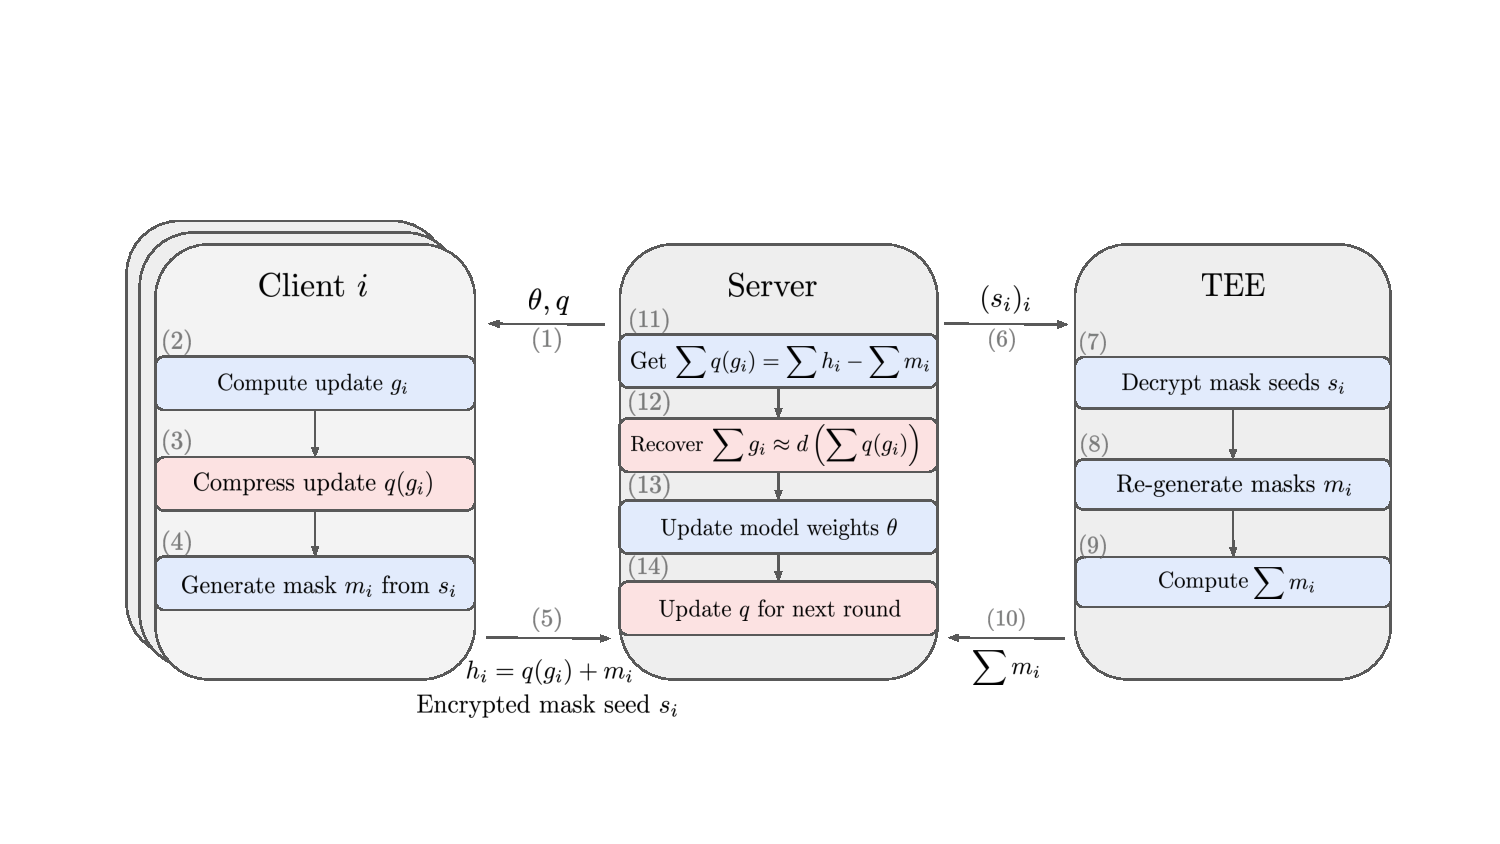
\includegraphics[width=0.8\textwidth]{figs/secagg_summary_new.pdf}
    %\vspace{-5mm}
    \caption{\label{fig:secagg_summary}
    Summary of the proposed approach for one FL round, where we omit the round dependency and \modif{Differential Privacy (DP)} for clarity. Blue boxes denote standard steps and red boxes denote additional steps for uplink compression. Client $i$ computes local model update $g_i$, compresses it with the compression operator $q$, and encrypts it by adding a random mask $m_i$ in the compressed domain, hence reducing the uplink bandwidth (steps 2--4). The server recovers the aggregate in the compressed domain by leveraging any \SecAgg protocol \modif{(steps 7--13, with a TEE-based \SecAgg, see Section~\ref{subsec:secagg})}. Since the decompression operator $d$ is linear, the server can convert the aggregate back to the non-compressed domain, up to compression error (step 12). As with the model weights $\theta$, the compression operator $q$ are also periodically updated and broadcast by the server (step 14). 
    In Section~\ref{sec:method}, we apply the proposed method to scalar quantization and pruning without impacting \SecAgg and propose Secure Indexing, a variant of \SecAgg for extreme uplink compression with product quantization. See Section~\ref{subsec:secagg} for details about \SecAgg and Section~\ref{sec:discussion} for a discussion on~DP.
    }
    \vspace{-3mm}
\end{figure*}



% Our focus in this paper is on 

%Second, scaling cross-device (synchronous) FL to millions of clients with various capabilities and intermittent availability \citep{bonavitz2019federated} suffers from diminishing returns: the wall-clock training time plateaus as the number of clients keeps increasing~\citep{huba2021papaya}. Even though this challenge can be addressed by leveraging the buffered asynchronous aggregation technique proposed by \cite{nguyen2021federated}, compatible with DP and SecAgg, the asynchronous protocol remains bottlenecked by communication latency between the server and the clients.


%Considering the above privacy and scalability goals, we focus on enabling efficient FL communications while keeping a high privacy bar. In addition to the primary objective of speeding up convergence, reducing communication costs brings other significant benefits. Lowering communication requirements addresses selection bias due to undersampling clients with limited connectivity, improving fairness and inclusivity metrics. Better communication efficiency shrinks the carbon footprint of FL, whose fraction attributable to communication can reach 95\%~\citep{qiu2021first}. %Finally, training larger model in FL would be a possibility, when the communication cost is reduced, because local memory or compute requirements can be addressed by modifying the local training loop, for instance with gradient checkpointing \citep{chen2016training}. However, some form of compression would be required to enable efficient communication.


%First, compressing model updates from the client to the server presents several challenges due to compatibility with SecAgg and is an area suitable for further research. 
%Second, upload bandwidth is generally more restricted than download. For instance, according to the most recent FCC report, the ratio of download to upload speeds for DSL/cable providers in the US ranges between 3$\times$ to 20$\times$~\citep{fcc-broadband}. We consider broadband speeds here because devices participate in the FL training while connected to fixed broadband, usually through Wi-Fi~\citep{huba2021papaya}.




% Hence, FL provides the ability to leverage data from massive client populations while ensuring the security and privacy of the client data.
% Go further: compatibility with DP / compression as a mitigation techniques of attacks
% Model and gradient compression intrinsically different.
%  Why not having the secure enclave perform the aggregation?
%%!TEX root = ../main.tex

\section{Concluding Remarks}
\label{conclusion}

There exist many systems for monitoring and analyzing spatio-temporal data, such as a dashboard for visually tracking the outbreak of COVID-19~\cite{dong2020interactive} and a tweet stream sentiment analysis system for US election 2016~\cite{DBLP:conf/kdd/PaulLTYF17}. 
One lesson from the existing systems is  that they are usually designed on a case-by-case basis and built from scratch, which cannot fully leverage the recent techniques for data integration and automatic visualization.

On the one side, \sys-COVID-19 shares many common visualizations as the other popular websites for tracking COVID-19 cases.
On the other side, it differs from the others in 
(1) \sys-COVID-19 is based on a general end-to-end framework \sys, and leverages recent techniques for data preparation (\eg~{\sc VisClean}~\cite{visclean-icde}) and for visualization recommendation (\eg~{\sc DeepEye}~\cite{deepeyeicde});
%
(2) it supports linked visualization for the users to easily zoom in/out multiple visualizations by a single click; and
%
(3) it also obtains some private data that is not publicly available, so it can demonstrate some unique features.
%
%Hopefully we can survive the war of fighting COVID-19 with the minimum cost, and by the time of VLDB 2020, we will have much more to demonstrate.

%\add{Open Challenges: (1) Smart and Effective Data Preparation. (2) Data Sharing Platform. (3) Intelligent Data Analysis (4) Abstract general modules, the system supports reusability}





% Optional math commands from https://github.com/goodfeli/dlbook_notation.
%%%%%% NEW MATH DEFINITIONS %%%%%

\usepackage{amsmath,amsfonts,bm}

% Mark sections of captions for referring to divisions of figures
\newcommand{\figleft}{{\em (Left)}}
\newcommand{\figcenter}{{\em (Center)}}
\newcommand{\figright}{{\em (Right)}}
\newcommand{\figtop}{{\em (Top)}}
\newcommand{\figbottom}{{\em (Bottom)}}
\newcommand{\captiona}{{\em (a)}}
\newcommand{\captionb}{{\em (b)}}
\newcommand{\captionc}{{\em (c)}}
\newcommand{\captiond}{{\em (d)}}

% Highlight a newly defined term
\newcommand{\newterm}[1]{{\bf #1}}


% Figure reference, lower-case.
\def\figref#1{figure~\ref{#1}}
% Figure reference, capital. For start of sentence
\def\Figref#1{Figure~\ref{#1}}
\def\twofigref#1#2{figures \ref{#1} and \ref{#2}}
\def\quadfigref#1#2#3#4{figures \ref{#1}, \ref{#2}, \ref{#3} and \ref{#4}}
% Section reference, lower-case.
\def\secref#1{section~\ref{#1}}
% Section reference, capital.
\def\Secref#1{Section~\ref{#1}}
% Reference to two sections.
\def\twosecrefs#1#2{sections \ref{#1} and \ref{#2}}
% Reference to three sections.
\def\secrefs#1#2#3{sections \ref{#1}, \ref{#2} and \ref{#3}}
% Reference to an equation, lower-case.
\def\eqref#1{equation~\ref{#1}}
% Reference to an equation, upper case
\def\Eqref#1{Equation~\ref{#1}}
% A raw reference to an equation---avoid using if possible
\def\plaineqref#1{\ref{#1}}
% Reference to a chapter, lower-case.
\def\chapref#1{chapter~\ref{#1}}
% Reference to an equation, upper case.
\def\Chapref#1{Chapter~\ref{#1}}
% Reference to a range of chapters
\def\rangechapref#1#2{chapters\ref{#1}--\ref{#2}}
% Reference to an algorithm, lower-case.
\def\algref#1{algorithm~\ref{#1}}
% Reference to an algorithm, upper case.
\def\Algref#1{Algorithm~\ref{#1}}
\def\twoalgref#1#2{algorithms \ref{#1} and \ref{#2}}
\def\Twoalgref#1#2{Algorithms \ref{#1} and \ref{#2}}
% Reference to a part, lower case
\def\partref#1{part~\ref{#1}}
% Reference to a part, upper case
\def\Partref#1{Part~\ref{#1}}
\def\twopartref#1#2{parts \ref{#1} and \ref{#2}}

\def\ceil#1{\lceil #1 \rceil}
\def\floor#1{\lfloor #1 \rfloor}
\def\1{\bm{1}}
\newcommand{\train}{\mathcal{D}}
\newcommand{\valid}{\mathcal{D_{\mathrm{valid}}}}
\newcommand{\test}{\mathcal{D_{\mathrm{test}}}}

\def\eps{{\epsilon}}


% Random variables
\def\reta{{\textnormal{$\eta$}}}
\def\ra{{\textnormal{a}}}
\def\rb{{\textnormal{b}}}
\def\rc{{\textnormal{c}}}
\def\rd{{\textnormal{d}}}
\def\re{{\textnormal{e}}}
\def\rf{{\textnormal{f}}}
\def\rg{{\textnormal{g}}}
\def\rh{{\textnormal{h}}}
\def\ri{{\textnormal{i}}}
\def\rj{{\textnormal{j}}}
\def\rk{{\textnormal{k}}}
\def\rl{{\textnormal{l}}}
% rm is already a command, just don't name any random variables m
\def\rn{{\textnormal{n}}}
\def\ro{{\textnormal{o}}}
\def\rp{{\textnormal{p}}}
\def\rq{{\textnormal{q}}}
\def\rr{{\textnormal{r}}}
\def\rs{{\textnormal{s}}}
\def\rt{{\textnormal{t}}}
\def\ru{{\textnormal{u}}}
\def\rv{{\textnormal{v}}}
\def\rw{{\textnormal{w}}}
\def\rx{{\textnormal{x}}}
\def\ry{{\textnormal{y}}}
\def\rz{{\textnormal{z}}}

% Random vectors
\def\rvepsilon{{\mathbf{\epsilon}}}
\def\rvtheta{{\mathbf{\theta}}}
\def\rva{{\mathbf{a}}}
\def\rvb{{\mathbf{b}}}
\def\rvc{{\mathbf{c}}}
\def\rvd{{\mathbf{d}}}
\def\rve{{\mathbf{e}}}
\def\rvf{{\mathbf{f}}}
\def\rvg{{\mathbf{g}}}
\def\rvh{{\mathbf{h}}}
\def\rvu{{\mathbf{i}}}
\def\rvj{{\mathbf{j}}}
\def\rvk{{\mathbf{k}}}
\def\rvl{{\mathbf{l}}}
\def\rvm{{\mathbf{m}}}
\def\rvn{{\mathbf{n}}}
\def\rvo{{\mathbf{o}}}
\def\rvp{{\mathbf{p}}}
\def\rvq{{\mathbf{q}}}
\def\rvr{{\mathbf{r}}}
\def\rvs{{\mathbf{s}}}
\def\rvt{{\mathbf{t}}}
\def\rvu{{\mathbf{u}}}
\def\rvv{{\mathbf{v}}}
\def\rvw{{\mathbf{w}}}
\def\rvx{{\mathbf{x}}}
\def\rvy{{\mathbf{y}}}
\def\rvz{{\mathbf{z}}}

% Elements of random vectors
\def\erva{{\textnormal{a}}}
\def\ervb{{\textnormal{b}}}
\def\ervc{{\textnormal{c}}}
\def\ervd{{\textnormal{d}}}
\def\erve{{\textnormal{e}}}
\def\ervf{{\textnormal{f}}}
\def\ervg{{\textnormal{g}}}
\def\ervh{{\textnormal{h}}}
\def\ervi{{\textnormal{i}}}
\def\ervj{{\textnormal{j}}}
\def\ervk{{\textnormal{k}}}
\def\ervl{{\textnormal{l}}}
\def\ervm{{\textnormal{m}}}
\def\ervn{{\textnormal{n}}}
\def\ervo{{\textnormal{o}}}
\def\ervp{{\textnormal{p}}}
\def\ervq{{\textnormal{q}}}
\def\ervr{{\textnormal{r}}}
\def\ervs{{\textnormal{s}}}
\def\ervt{{\textnormal{t}}}
\def\ervu{{\textnormal{u}}}
\def\ervv{{\textnormal{v}}}
\def\ervw{{\textnormal{w}}}
\def\ervx{{\textnormal{x}}}
\def\ervy{{\textnormal{y}}}
\def\ervz{{\textnormal{z}}}

% Random matrices
\def\rmA{{\mathbf{A}}}
\def\rmB{{\mathbf{B}}}
\def\rmC{{\mathbf{C}}}
\def\rmD{{\mathbf{D}}}
\def\rmE{{\mathbf{E}}}
\def\rmF{{\mathbf{F}}}
\def\rmG{{\mathbf{G}}}
\def\rmH{{\mathbf{H}}}
\def\rmI{{\mathbf{I}}}
\def\rmJ{{\mathbf{J}}}
\def\rmK{{\mathbf{K}}}
\def\rmL{{\mathbf{L}}}
\def\rmM{{\mathbf{M}}}
\def\rmN{{\mathbf{N}}}
\def\rmO{{\mathbf{O}}}
\def\rmP{{\mathbf{P}}}
\def\rmQ{{\mathbf{Q}}}
\def\rmR{{\mathbf{R}}}
\def\rmS{{\mathbf{S}}}
\def\rmT{{\mathbf{T}}}
\def\rmU{{\mathbf{U}}}
\def\rmV{{\mathbf{V}}}
\def\rmW{{\mathbf{W}}}
\def\rmX{{\mathbf{X}}}
\def\rmY{{\mathbf{Y}}}
\def\rmZ{{\mathbf{Z}}}

% Elements of random matrices
\def\ermA{{\textnormal{A}}}
\def\ermB{{\textnormal{B}}}
\def\ermC{{\textnormal{C}}}
\def\ermD{{\textnormal{D}}}
\def\ermE{{\textnormal{E}}}
\def\ermF{{\textnormal{F}}}
\def\ermG{{\textnormal{G}}}
\def\ermH{{\textnormal{H}}}
\def\ermI{{\textnormal{I}}}
\def\ermJ{{\textnormal{J}}}
\def\ermK{{\textnormal{K}}}
\def\ermL{{\textnormal{L}}}
\def\ermM{{\textnormal{M}}}
\def\ermN{{\textnormal{N}}}
\def\ermO{{\textnormal{O}}}
\def\ermP{{\textnormal{P}}}
\def\ermQ{{\textnormal{Q}}}
\def\ermR{{\textnormal{R}}}
\def\ermS{{\textnormal{S}}}
\def\ermT{{\textnormal{T}}}
\def\ermU{{\textnormal{U}}}
\def\ermV{{\textnormal{V}}}
\def\ermW{{\textnormal{W}}}
\def\ermX{{\textnormal{X}}}
\def\ermY{{\textnormal{Y}}}
\def\ermZ{{\textnormal{Z}}}

% Vectors
\def\vzero{{\bm{0}}}
\def\vone{{\bm{1}}}
\def\vmu{{\bm{\mu}}}
\def\vtheta{{\bm{\theta}}}
\def\va{{\bm{a}}}
\def\vb{{\bm{b}}}
\def\vc{{\bm{c}}}
\def\vd{{\bm{d}}}
\def\ve{{\bm{e}}}
\def\vf{{\bm{f}}}
\def\vg{{\bm{g}}}
\def\vh{{\bm{h}}}
\def\vi{{\bm{i}}}
\def\vj{{\bm{j}}}
\def\vk{{\bm{k}}}
\def\vl{{\bm{l}}}
\def\vm{{\bm{m}}}
\def\vn{{\bm{n}}}
\def\vo{{\bm{o}}}
\def\vp{{\bm{p}}}
\def\vq{{\bm{q}}}
\def\vr{{\bm{r}}}
\def\vs{{\bm{s}}}
\def\vt{{\bm{t}}}
\def\vu{{\bm{u}}}
\def\vv{{\bm{v}}}
\def\vw{{\bm{w}}}
\def\vx{{\bm{x}}}
\def\vy{{\bm{y}}}
\def\vz{{\bm{z}}}

% Elements of vectors
\def\evalpha{{\alpha}}
\def\evbeta{{\beta}}
\def\evepsilon{{\epsilon}}
\def\evlambda{{\lambda}}
\def\evomega{{\omega}}
\def\evmu{{\mu}}
\def\evpsi{{\psi}}
\def\evsigma{{\sigma}}
\def\evtheta{{\theta}}
\def\eva{{a}}
\def\evb{{b}}
\def\evc{{c}}
\def\evd{{d}}
\def\eve{{e}}
\def\evf{{f}}
\def\evg{{g}}
\def\evh{{h}}
\def\evi{{i}}
\def\evj{{j}}
\def\evk{{k}}
\def\evl{{l}}
\def\evm{{m}}
\def\evn{{n}}
\def\evo{{o}}
\def\evp{{p}}
\def\evq{{q}}
\def\evr{{r}}
\def\evs{{s}}
\def\evt{{t}}
\def\evu{{u}}
\def\evv{{v}}
\def\evw{{w}}
\def\evx{{x}}
\def\evy{{y}}
\def\evz{{z}}

% Matrix
\def\mA{{\bm{A}}}
\def\mB{{\bm{B}}}
\def\mC{{\bm{C}}}
\def\mD{{\bm{D}}}
\def\mE{{\bm{E}}}
\def\mF{{\bm{F}}}
\def\mG{{\bm{G}}}
\def\mH{{\bm{H}}}
\def\mI{{\bm{I}}}
\def\mJ{{\bm{J}}}
\def\mK{{\bm{K}}}
\def\mL{{\bm{L}}}
\def\mM{{\bm{M}}}
\def\mN{{\bm{N}}}
\def\mO{{\bm{O}}}
\def\mP{{\bm{P}}}
\def\mQ{{\bm{Q}}}
\def\mR{{\bm{R}}}
\def\mS{{\bm{S}}}
\def\mT{{\bm{T}}}
\def\mU{{\bm{U}}}
\def\mV{{\bm{V}}}
\def\mW{{\bm{W}}}
\def\mX{{\bm{X}}}
\def\mY{{\bm{Y}}}
\def\mZ{{\bm{Z}}}
\def\mBeta{{\bm{\beta}}}
\def\mPhi{{\bm{\Phi}}}
\def\mLambda{{\bm{\Lambda}}}
\def\mSigma{{\bm{\Sigma}}}

% Tensor
\DeclareMathAlphabet{\mathsfit}{\encodingdefault}{\sfdefault}{m}{sl}
\SetMathAlphabet{\mathsfit}{bold}{\encodingdefault}{\sfdefault}{bx}{n}
\newcommand{\tens}[1]{\bm{\mathsfit{#1}}}
\def\tA{{\tens{A}}}
\def\tB{{\tens{B}}}
\def\tC{{\tens{C}}}
\def\tD{{\tens{D}}}
\def\tE{{\tens{E}}}
\def\tF{{\tens{F}}}
\def\tG{{\tens{G}}}
\def\tH{{\tens{H}}}
\def\tI{{\tens{I}}}
\def\tJ{{\tens{J}}}
\def\tK{{\tens{K}}}
\def\tL{{\tens{L}}}
\def\tM{{\tens{M}}}
\def\tN{{\tens{N}}}
\def\tO{{\tens{O}}}
\def\tP{{\tens{P}}}
\def\tQ{{\tens{Q}}}
\def\tR{{\tens{R}}}
\def\tS{{\tens{S}}}
\def\tT{{\tens{T}}}
\def\tU{{\tens{U}}}
\def\tV{{\tens{V}}}
\def\tW{{\tens{W}}}
\def\tX{{\tens{X}}}
\def\tY{{\tens{Y}}}
\def\tZ{{\tens{Z}}}


% Graph
\def\gA{{\mathcal{A}}}
\def\gB{{\mathcal{B}}}
\def\gC{{\mathcal{C}}}
\def\gD{{\mathcal{D}}}
\def\gE{{\mathcal{E}}}
\def\gF{{\mathcal{F}}}
\def\gG{{\mathcal{G}}}
\def\gH{{\mathcal{H}}}
\def\gI{{\mathcal{I}}}
\def\gJ{{\mathcal{J}}}
\def\gK{{\mathcal{K}}}
\def\gL{{\mathcal{L}}}
\def\gM{{\mathcal{M}}}
\def\gN{{\mathcal{N}}}
\def\gO{{\mathcal{O}}}
\def\gP{{\mathcal{P}}}
\def\gQ{{\mathcal{Q}}}
\def\gR{{\mathcal{R}}}
\def\gS{{\mathcal{S}}}
\def\gT{{\mathcal{T}}}
\def\gU{{\mathcal{U}}}
\def\gV{{\mathcal{V}}}
\def\gW{{\mathcal{W}}}
\def\gX{{\mathcal{X}}}
\def\gY{{\mathcal{Y}}}
\def\gZ{{\mathcal{Z}}}

% Sets
\def\sA{{\mathbb{A}}}
\def\sB{{\mathbb{B}}}
\def\sC{{\mathbb{C}}}
\def\sD{{\mathbb{D}}}
% Don't use a set called E, because this would be the same as our symbol
% for expectation.
\def\sF{{\mathbb{F}}}
\def\sG{{\mathbb{G}}}
\def\sH{{\mathbb{H}}}
\def\sI{{\mathbb{I}}}
\def\sJ{{\mathbb{J}}}
\def\sK{{\mathbb{K}}}
\def\sL{{\mathbb{L}}}
\def\sM{{\mathbb{M}}}
\def\sN{{\mathbb{N}}}
\def\sO{{\mathbb{O}}}
\def\sP{{\mathbb{P}}}
\def\sQ{{\mathbb{Q}}}
\def\sR{{\mathbb{R}}}
\def\sS{{\mathbb{S}}}
\def\sT{{\mathbb{T}}}
\def\sU{{\mathbb{U}}}
\def\sV{{\mathbb{V}}}
\def\sW{{\mathbb{W}}}
\def\sX{{\mathbb{X}}}
\def\sY{{\mathbb{Y}}}
\def\sZ{{\mathbb{Z}}}

% Entries of a matrix
\def\emLambda{{\Lambda}}
\def\emA{{A}}
\def\emB{{B}}
\def\emC{{C}}
\def\emD{{D}}
\def\emE{{E}}
\def\emF{{F}}
\def\emG{{G}}
\def\emH{{H}}
\def\emI{{I}}
\def\emJ{{J}}
\def\emK{{K}}
\def\emL{{L}}
\def\emM{{M}}
\def\emN{{N}}
\def\emO{{O}}
\def\emP{{P}}
\def\emQ{{Q}}
\def\emR{{R}}
\def\emS{{S}}
\def\emT{{T}}
\def\emU{{U}}
\def\emV{{V}}
\def\emW{{W}}
\def\emX{{X}}
\def\emY{{Y}}
\def\emZ{{Z}}
\def\emSigma{{\Sigma}}

% entries of a tensor
% Same font as tensor, without \bm wrapper
\newcommand{\etens}[1]{\mathsfit{#1}}
\def\etLambda{{\etens{\Lambda}}}
\def\etA{{\etens{A}}}
\def\etB{{\etens{B}}}
\def\etC{{\etens{C}}}
\def\etD{{\etens{D}}}
\def\etE{{\etens{E}}}
\def\etF{{\etens{F}}}
\def\etG{{\etens{G}}}
\def\etH{{\etens{H}}}
\def\etI{{\etens{I}}}
\def\etJ{{\etens{J}}}
\def\etK{{\etens{K}}}
\def\etL{{\etens{L}}}
\def\etM{{\etens{M}}}
\def\etN{{\etens{N}}}
\def\etO{{\etens{O}}}
\def\etP{{\etens{P}}}
\def\etQ{{\etens{Q}}}
\def\etR{{\etens{R}}}
\def\etS{{\etens{S}}}
\def\etT{{\etens{T}}}
\def\etU{{\etens{U}}}
\def\etV{{\etens{V}}}
\def\etW{{\etens{W}}}
\def\etX{{\etens{X}}}
\def\etY{{\etens{Y}}}
\def\etZ{{\etens{Z}}}

% The true underlying data generating distribution
\newcommand{\pdata}{p_{\rm{data}}}
% The empirical distribution defined by the training set
\newcommand{\ptrain}{\hat{p}_{\rm{data}}}
\newcommand{\Ptrain}{\hat{P}_{\rm{data}}}
% The model distribution
\newcommand{\pmodel}{p_{\rm{model}}}
\newcommand{\Pmodel}{P_{\rm{model}}}
\newcommand{\ptildemodel}{\tilde{p}_{\rm{model}}}
% Stochastic autoencoder distributions
\newcommand{\pencode}{p_{\rm{encoder}}}
\newcommand{\pdecode}{p_{\rm{decoder}}}
\newcommand{\precons}{p_{\rm{reconstruct}}}

\newcommand{\laplace}{\mathrm{Laplace}} % Laplace distribution

\newcommand{\E}{\mathbb{E}}
\newcommand{\Ls}{\mathcal{L}}
\newcommand{\R}{\mathbb{R}}
\newcommand{\emp}{\tilde{p}}
\newcommand{\lr}{\alpha}
\newcommand{\reg}{\lambda}
\newcommand{\rect}{\mathrm{rectifier}}
\newcommand{\softmax}{\mathrm{softmax}}
\newcommand{\sigmoid}{\sigma}
\newcommand{\softplus}{\zeta}
\newcommand{\KL}{D_{\mathrm{KL}}}
\newcommand{\Var}{\mathrm{Var}}
\newcommand{\standarderror}{\mathrm{SE}}
\newcommand{\Cov}{\mathrm{Cov}}
% Wolfram Mathworld says $L^2$ is for function spaces and $\ell^2$ is for vectors
% But then they seem to use $L^2$ for vectors throughout the site, and so does
% wikipedia.
\newcommand{\normlzero}{L^0}
\newcommand{\normlone}{L^1}
\newcommand{\normltwo}{L^2}
\newcommand{\normlp}{L^p}
\newcommand{\normmax}{L^\infty}

\newcommand{\parents}{Pa} % See usage in notation.tex. Chosen to match Daphne's book.

\DeclareMathOperator*{\argmax}{arg\,max}
\DeclareMathOperator*{\argmin}{arg\,min}

\DeclareMathOperator{\sign}{sign}
\DeclareMathOperator{\Tr}{Tr}
\let\ab\allowbreak


% Recommended, but optional, packages for figures and better typesetting:

\newcommand{\todoir}[2]{}
\newcommand{\irnote}[1]{\todoir{red}{IR: ``#1''}}
\newcommand{\pinote}[1]{\todoir{blue}{PI: ``#1''}}
\newcommand{\twnote}[1]{\todoir{orange}{TW: ``#1''}}
\newcommand{\ynote}[1]{\todoir{cyan}{YD: ``#1''}}


% Attempt to make hyperref and algorithmic work together better:
\newcommand{\theHalgorithm}{\arabic{algorithm}}

\newcommand{\R}{\mathbb R}
\newcommand\Rbb{\ensuremath{\mathbb{R}}} 

\iffalse
\title{My Title}

\author{Name1$\dagger$\footnote{work done while working at home}, Name2*, Name3$\ddagger$$^*$, \\ Name4*\\
  *University of Earth \\
  $\dagger$Moon University, email@moon.edu \\
  $\ddagger$University of Mars, email@mars.edu\\
  *{email2, email4}@earth.com
}

\fi


\begin{document}

\title{Learning Space Partitions for Nearest Neighbor Search}


\author{
  Yihe Dong$^\dagger$, 
  Piotr Indyk$^\ddagger$, 
  Ilya Razenshteyn$^\S$, 
  Tal Wagner$^\parallel$ \\
  $^\dagger$Work done at Microsoft Research. Now at Google.\\
  $^\ddagger$MIT.\\
  $^\S$Work done at Microsoft Research. Now at Pyte.\\
  $^\parallel$Work done at Microsoft Research and MIT. Now at Amazon and Tel-Aviv University.\\
  \ \\
  Author names are ordered alphabetically.\\
}



\maketitle
\renewcommand\thesection{\arabic{section}}
\setcounter{section}{0}
\setcounter{figure}{0}
\setcounter{table}{0}
\begin{abstract}
Space partitions of $\mathbb{R}^d$ underlie a vast and important
class of fast nearest neighbor search (NNS) algorithms.
Inspired by recent theoretical work on NNS for general metric spaces~\cite{andoni2018data,andoni2018holder}, we develop a new framework for building space partitions reducing the problem
to \emph{balanced graph partitioning} followed by
\emph{supervised classification.}
We instantiate this general approach with the KaHIP graph partitioner~\cite{sandersschulz2013} and neural networks,
respectively,
to obtain a new partitioning procedure called \emph{Neural Locality-Sensitive Hashing (Neural LSH).}
On several standard benchmarks for NNS~\cite{aumuller2017ann}, our experiments show that the partitions obtained by Neural LSH consistently outperform partitions found by quantization-based and tree-based methods as well as classic, data-oblivious LSH.
\end{abstract}

\section{Introduction}

%\irnote{Add a sentence about scaling.}

The {\it Nearest Neighbor Search (NNS)} problem is defined as follows. Given an $n$-point dataset $P$ in a $d$-dimensional Euclidean space $\mathbb{R}^d$, we would like to preprocess $P$ to answer $k$-nearest neighbor queries quickly.
That is, given a query point $q \in \mathbb{R}^d$, we want to find the $k$ data points from $P$
that are closest to $q$. NNS is a cornerstone of the modern data analysis and, at the same time, a fundamental geometric data structure problem that led to many exciting theoretical developments over the past decades. See, e.g., \cite{wang2016learning,andoni2018approximate} for an overview.

The main two approaches to constructing efficient NNS data structures are \emph{indexing} and \emph{sketching}. The goal of indexing is to construct a data structure that, given a query point, produces a small subset of $P$ (called  \emph{candidate set}) that includes the desired neighbors. Such a data structure can be stored on a single machine,  or (if the data set is very large) distributed among  multiple machines. In contrast, the goal of sketching is to compute compressed representations  of points to enable computing approximate distances quickly (e.g., compact binary hash codes with the Hamming distance used as an estimator, see the surveys~\cite{wang2014hashing,wang2016learning}). 
Indexing and sketching can be (and often are) combined to maximize the overall performance \cite{wu2017multiscale,johnson2017billion}.

Both indexing and sketching have been the topic of a vast amount of theoretical and empirical literature.
In this work, we consider the \emph{indexing} problem. In particular, we focus on indexing  based on \emph{space partitions}.
The overarching idea is to build a partition of the ambient space $\mathbb{R}^d$ and split the dataset $P$ accordingly.
Given a query point  $q$, we identify the bin containing $q$ and
form the resulting list of candidates from the data points residing in the same bin (or, to boost the accuracy, nearby bins as well).
%To boost the search accuracy, it is often necessary to add all data points from  \emph{nearby} bins to the candidate list
%(this is often referred as the \emph{multi-probe} technique).
%The literature about space partitions for NNS is so vast that it would be completely futile to try to give a thorough overview. Instead,
%we list the main classes of methods that have been showing great performance: 

Some of the popular space partitioning methods include the following:

\begin{itemize}
    \item {\em locality-sensitive hashing (LSH)} \cite{indyk1998approximate, andoni2008near,lv2007multi,andoni2015practical}, where the partitioning is obtained by hashing the points into ``bins'' such that the probability of two points colliding dependends on the distance between them,
    \item {\em quantization-based} approaches~\cite{jegou2011product,babenko2012inverted,avq_2020},
where partitions are obtained via $k$-means clustering of the dataset and its generalizations, and
    \item {\em tree-based} methods, such as  random-projection trees, learned trees or PCA trees~\cite{sproull1991refinements,bawa2005lsh,cayton2008learning, li2011learning,dasgupta2013randomized, keivani2018improved}. Here, the partition is defined by a rooted binary tree, where each internal node $v$ is augmented with a hyperplane, and each edge to a child of $v$ corresponds to one of the two halfspaces defined by the hyperplane.  In turn, each leaf $v$ in the tree corresponds to a cell in the partition, defined as the intersection of all halfspaces corresponding to the edges on a path from the root to $v$.
\end{itemize}

Compared to other indexing methods (see Section~\ref{piotr_sec:related}), space partitions have multiple benefits. First, they are naturally applicable in {\em distributed} settings, as different bins can be stored on different machines~\cite{bahmani2012efficient, nidetecting,  li2017losha, bhaskara2018distributed}. Moverover, the computational efficiency of search can be further improved by using any nearest neighbor search algorithm locally on each machine. Second, partition-based indexing is particularly suitable for GPUs due to the simple and predictable memory access pattern~\cite{johnson2017billion}. Finally, partitions can be combined with cryptographic techniques to yield efficient {\em secure} similarity search algorithms~\cite{chen2019sanns}. Thus, in this paper we focus on designing space partitions that optimize the trade-off between their key metrics: the number of reported candidates, the fraction of the true nearest neighbors among the candidates, the number of bins, and the computational efficiency of the point location.


Recently, there has been a large body of work that studies how modern machine learning
techniques (such as neural networks) can help tackle various classic algorithmic problems (a partial list includes~\cite{mousavi2015deep,bora2017compressed,khalil2017learning,kraska2017case, balcan2018learning,lykouris2018competitive,mitz2018model,purohit2018improving}).
Similar methods---under the name ``learn to hash''---have been used to improve the \emph{sketching} approach to NNS~\cite{wang2016learning}. 
%However, when it comes to \emph{indexing}, only rather simple unsupervised techniques such as PCA or $k$-means have been (successfully) used.
%\irnote{This might have triggered the reviewer who mentioned learned kd-trees. I think we need to reformulate this sentence.}\twnote{Suggestion:}
However, when it comes to~\emph{indexing}, while some unsupervised techniques such as PCA or $k$-means have been successfully applied, the full power of modern tools like neural networks has not yet been harnessed. This state of affairs naturally
leads to the following general question:
    \textbf{Can we employ modern (supervised) machine learning techniques
    to find good space partitions for nearest neighbor search?}

%\irnote{The following paragraph needs to be fixed!}
%Recent work has shown that supervised machine learning methods, such as neural networks, can be used to obtain improved solutions for various classic algorithmic problems, including nearest neighbor search~\cite{wang2016learning,kraska2017case, balcan2018learning,lykouris2018competitive,mitz2018model}. However, even though these methods have been applied to the  \emph{sketching} approach  (more on this below), we are not aware of any successful attempts to do the same for the \emph{indexing} approach.
%This state of affairs naturally leads to the following question: 
%
%\begin{center}
%    \textbf{Can we employ (supervised) machine learning
%    techniques
%    to find good space partitions for nearest neighbor search?}
%\end{center}



\subsection{Our contribution}

In this paper we address the aforementioned challenge and present a new framework for finding high-quality space partitions of $\mathbb{R}^d$.
Our approach consists of three major steps:
\begin{CompactEnumerate}
\item Build the $k$-NN graph $G$ of the dataset by connecting each data point to $k$ nearest neighbors;
\item Find a balanced partition $\mathcal{P}$ of the graph $G$ into $m$ parts of nearly-equal size such that the number of edges between different parts is as small as possible;
\item Obtain a partition of $\mathbb{R}^d$ by training a classifier on the data points with labels being the parts of the partition $\mathcal{P}$ found in the second step.
\end{CompactEnumerate}

See Figure~\ref{piotr_fig:pipeline} for illustration.
The new algorithm \emph{directly optimizes} the performance of the partition-based nearest neighbor data structure.
Indeed, if a query is chosen as a uniformly random \emph{data point,} then the average $k$-NN accuracy is exactly equal to the fraction of edges of the $k$-NN
graph $G$ whose endpoints are separated by the partition $\mathcal{P}$. This generalizes to out-of-sample queries provided that
the query and dataset distributions are close, and the test accuracy of the trained classifier is high.

At the same time, our approach is directly related to and inspired by recent theoretical work~\cite{andoni2018data,andoni2018holder} on NNS for general metric spaces.
In particular, using the framework of~\cite{andoni2018data,andoni2018holder}, we prove that, under mild conditions on the dataset $P$, the $k$-NN graph of $P$
can be partitioned with a hyperplane into two parts of comparable size such that only few edges get split by the hyperplane. This gives a partial theoretical justification of our method.

The new framework is very flexible and uses partitioning and learning in a black-box way. This 
    allows us to plug various models (linear models, neural networks,
    etc.) and explore the trade-off between the quality
    and the algorithmic efficiency of the resulting partitions.
We emphasize the importance of~\emph{balanced} partitions for the indexing problem, where all bins contain roughly the same number of data points.
This property is crucial in the distributed setting, since
we naturally would like to assign a similar number
of points to each machine. 
Furthermore, balanced partitions allow tighter control
of the number of candidates simply by varying the number of retrieved parts.
Note that a priori, it is unclear how to partition $\mathbb{R}^d$ so as to induce balanced bins of a given dataset. Here the combinatorial portion of our approach is particularly useful, as balanced graph partitioning is a well-studied problem, and our supervised extension to $\mathbb{R}^d$ naturally preserves the balance by virtue of attaining high training accuracy.

We speculate that the new method might be potentially useful for solving the NNS problem for \emph{non-Euclidean} metrics, such as the edit distance~\cite{zhang2017embedjoin} or optimal transport distance~\cite{kusner2015word}. Indeed, for any metric space,
one can compute the $k$-NN graph and then partition it. The only step
that needs to be adjusted to the specific metric at hand is the learning step.

Let us finally put forward the challenge of scaling our method up to billion-sized or
even
larger datasets. For such scale, one needs
to build an \emph{approximate} $k$-NN
graph as well as using graph partitioning algorithms
that are faster than KaHIP. We leave
this exciting direction to future work. For the current experiments (datasets of size $10^6$ points), preprocessing takes several hours.
%
Another important challenge is to obtain NNS algorithms
based on the above partitioning with \emph{provable}
guarantees in terms of approximation and running time. However, we expect it to be difficult,
in particular, since all the current state-of-the-art NNS algorithms lack such guarantees~(e.g., $k$-means-based~\cite{jegou2011product} or graph methods~\cite{malkov2018efficient}, see also \cite{aumuller2017ann} for a recent SOTA survey).

\paragraph{Evaluation} We instantiate our framework with the KaHIP algorithm~\cite{sandersschulz2013} for the graph partitioning step, and either linear models or small-size neural networks for the learning step.
We evaluate it on several standard benchmarks for NNS~\cite{aumuller2017ann} and conclude that in terms of quality of the resulting partitions, it consistently outperforms quantization-based and tree-based partitioning
procedures, while maintaining comparable algorithmic efficiency. In the high accuracy regime,
our framework yields partitions that lead to processing up to $2.3\times$ fewer candidates than the strongest baseline.

As a baseline method we use $k$-means clustering~\cite{jegou2011product}. It produces a partition of the dataset into $k$ bins, in a way that naturally extends to all of $\mathbb{R}^d$, by assigning a query point $q$ to its nearest centroid. (More generally, for multi-probe querying, we can rank the bins by the distance of their centroids to $q$). This simple scheme yields very high-quality results for indexing. Besides $k$-means, we evaluate LSH~\cite{andoni2015practical}, ITQ~\cite{gong2013iterative}, PCA tree~\cite{sproull1991refinements}, RP tree~\cite{dasgupta2013randomized}, and Neural Catalyzer~\cite{sablayrolles2018spreading}.

%Several algorithms in the latter class, such as 
\subsection{Related work}\label{piotr_sec:related}



On the empirical side, currently the fastest indexing methods for the NNS problem are \emph{greedy graph-based} algorithms, such as HNSW~\cite{malkov2018efficient}, NSG~\cite{fu2019fast} or DiskANN~\cite{jayaram2019diskann}.
Their high-level idea is to construct a graph on the dataset
(it can be the $k$-NN graph, but other constructions are also possible), and then for each query perform a walk, which eventually converges to the nearest neighbor.
Although very fast, graph-based approaches have suboptimal ``locality of reference'', which makes them less suitable for several modern architectures. For instance, this is the case when the algorithm is run on a GPU~\cite{johnson2017billion}, or when the data is stored in external memory~\cite{sun2014srs} or in a distributed manner~\cite{bahmani2012efficient,nidetecting}.
Moreover, graph-based indexing requires many rounds of adaptive access to the dataset, whereas partition-based indexing accesses the dataset in one shot.
This is crucial, for example, for nearest neighbor search over encrypted data~\cite{chen2019sanns}.
These benefits justify further study of partition-based methods.

Machine learning techniques are particularly useful for the \emph{sketching} approach, leading to a vast body of research 
under the label ``learning to hash''~\cite{wang2014hashing,wang2016learning}.
In particular, several recent works employed neural networks to obtain high-quality sketches~\cite{erin2015deep,sablayrolles2018spreading}.
The fundamental difference from our work is that sketching is designed to speed up~\emph{linear scans} over the dataset, by reducing the \emph{cost} of distance evaluation, while indexing is designed for~\emph{sublinear time} searches, by reducing the \emph{number} of distance evaluations.

We note that while sketches are not designed for indexing, they can be used for that purpose, since a $b$-bit hashing scheme induces a partition of $\R^d$ into $2^b$ parts.
%
Nonetheless, our experiments show that partitions induced by these methods (such as Iterative Quantization~\cite{gong2013iterative}) are not well-suited for indexing, and underperform compared to quantization-based indexing, as well as to our methods.

We highlight in particular the recent work of~\cite{sablayrolles2018spreading}, which uses neural networks to learn a mapping $f \colon \mathbb{R}^d \to \mathbb{R}^{d'}$
that improves the geometry of the dataset and the queries to facilitate subsequent sketching.
%It is natural to apply the same family of maps for \emph{partitions}; however,
It is natural to ask whether the same family of maps can be applied to enhance the quality of \emph{partitions} for indexing. However,
as our experiments show, in the high accuracy regime the maps learned using the algorithm of~\cite{sablayrolles2018spreading}
consistently degrade the quality of partitions.

%using partitions obtained this way for indexing is very different from the intended
%use of sketches, and we confirm experimentally that high-quality sketching techniques such as ITQ~\cite{gong2013iterative} produce partitions
%that underperform compared to quantization-based partitions as well as the framework we introduce in this paper.

%A different application of neural networks related to NNS is to optimize the performance of the nearest neighbor~\emph{classifier}.
%Given a labeled dataset in a classification setting, the idea is to learn a representation of the dataset -- either as sketches~\cite{klein2017defense,jain2017subic} or as a high-dimensional embedding~\cite{schmidt2018learning} -- that would render the nearest neighbor classifier (i.e., labeling each query point with the label of its nearest data point) as accurate as possible. Apart from not producing an indexing method, these works are also different from ours by being inherently supervised, relying on a fully labeled dataset, whereas our approach is unsupervised.

Finally, we mention that here is some prior work on learning space partitions: \cite{cayton2008learning,ram2013space,li2011learning}.
However, all these algorithms learn \emph{hyperplane} partitions into two parts (then applying them recursively).
Our method, on the other hand, is much more flexible, since neural networks allow us to learn a much richer class of partitions.

\begin{figure*}%
    \centering
    \subfloat[Dataset]{{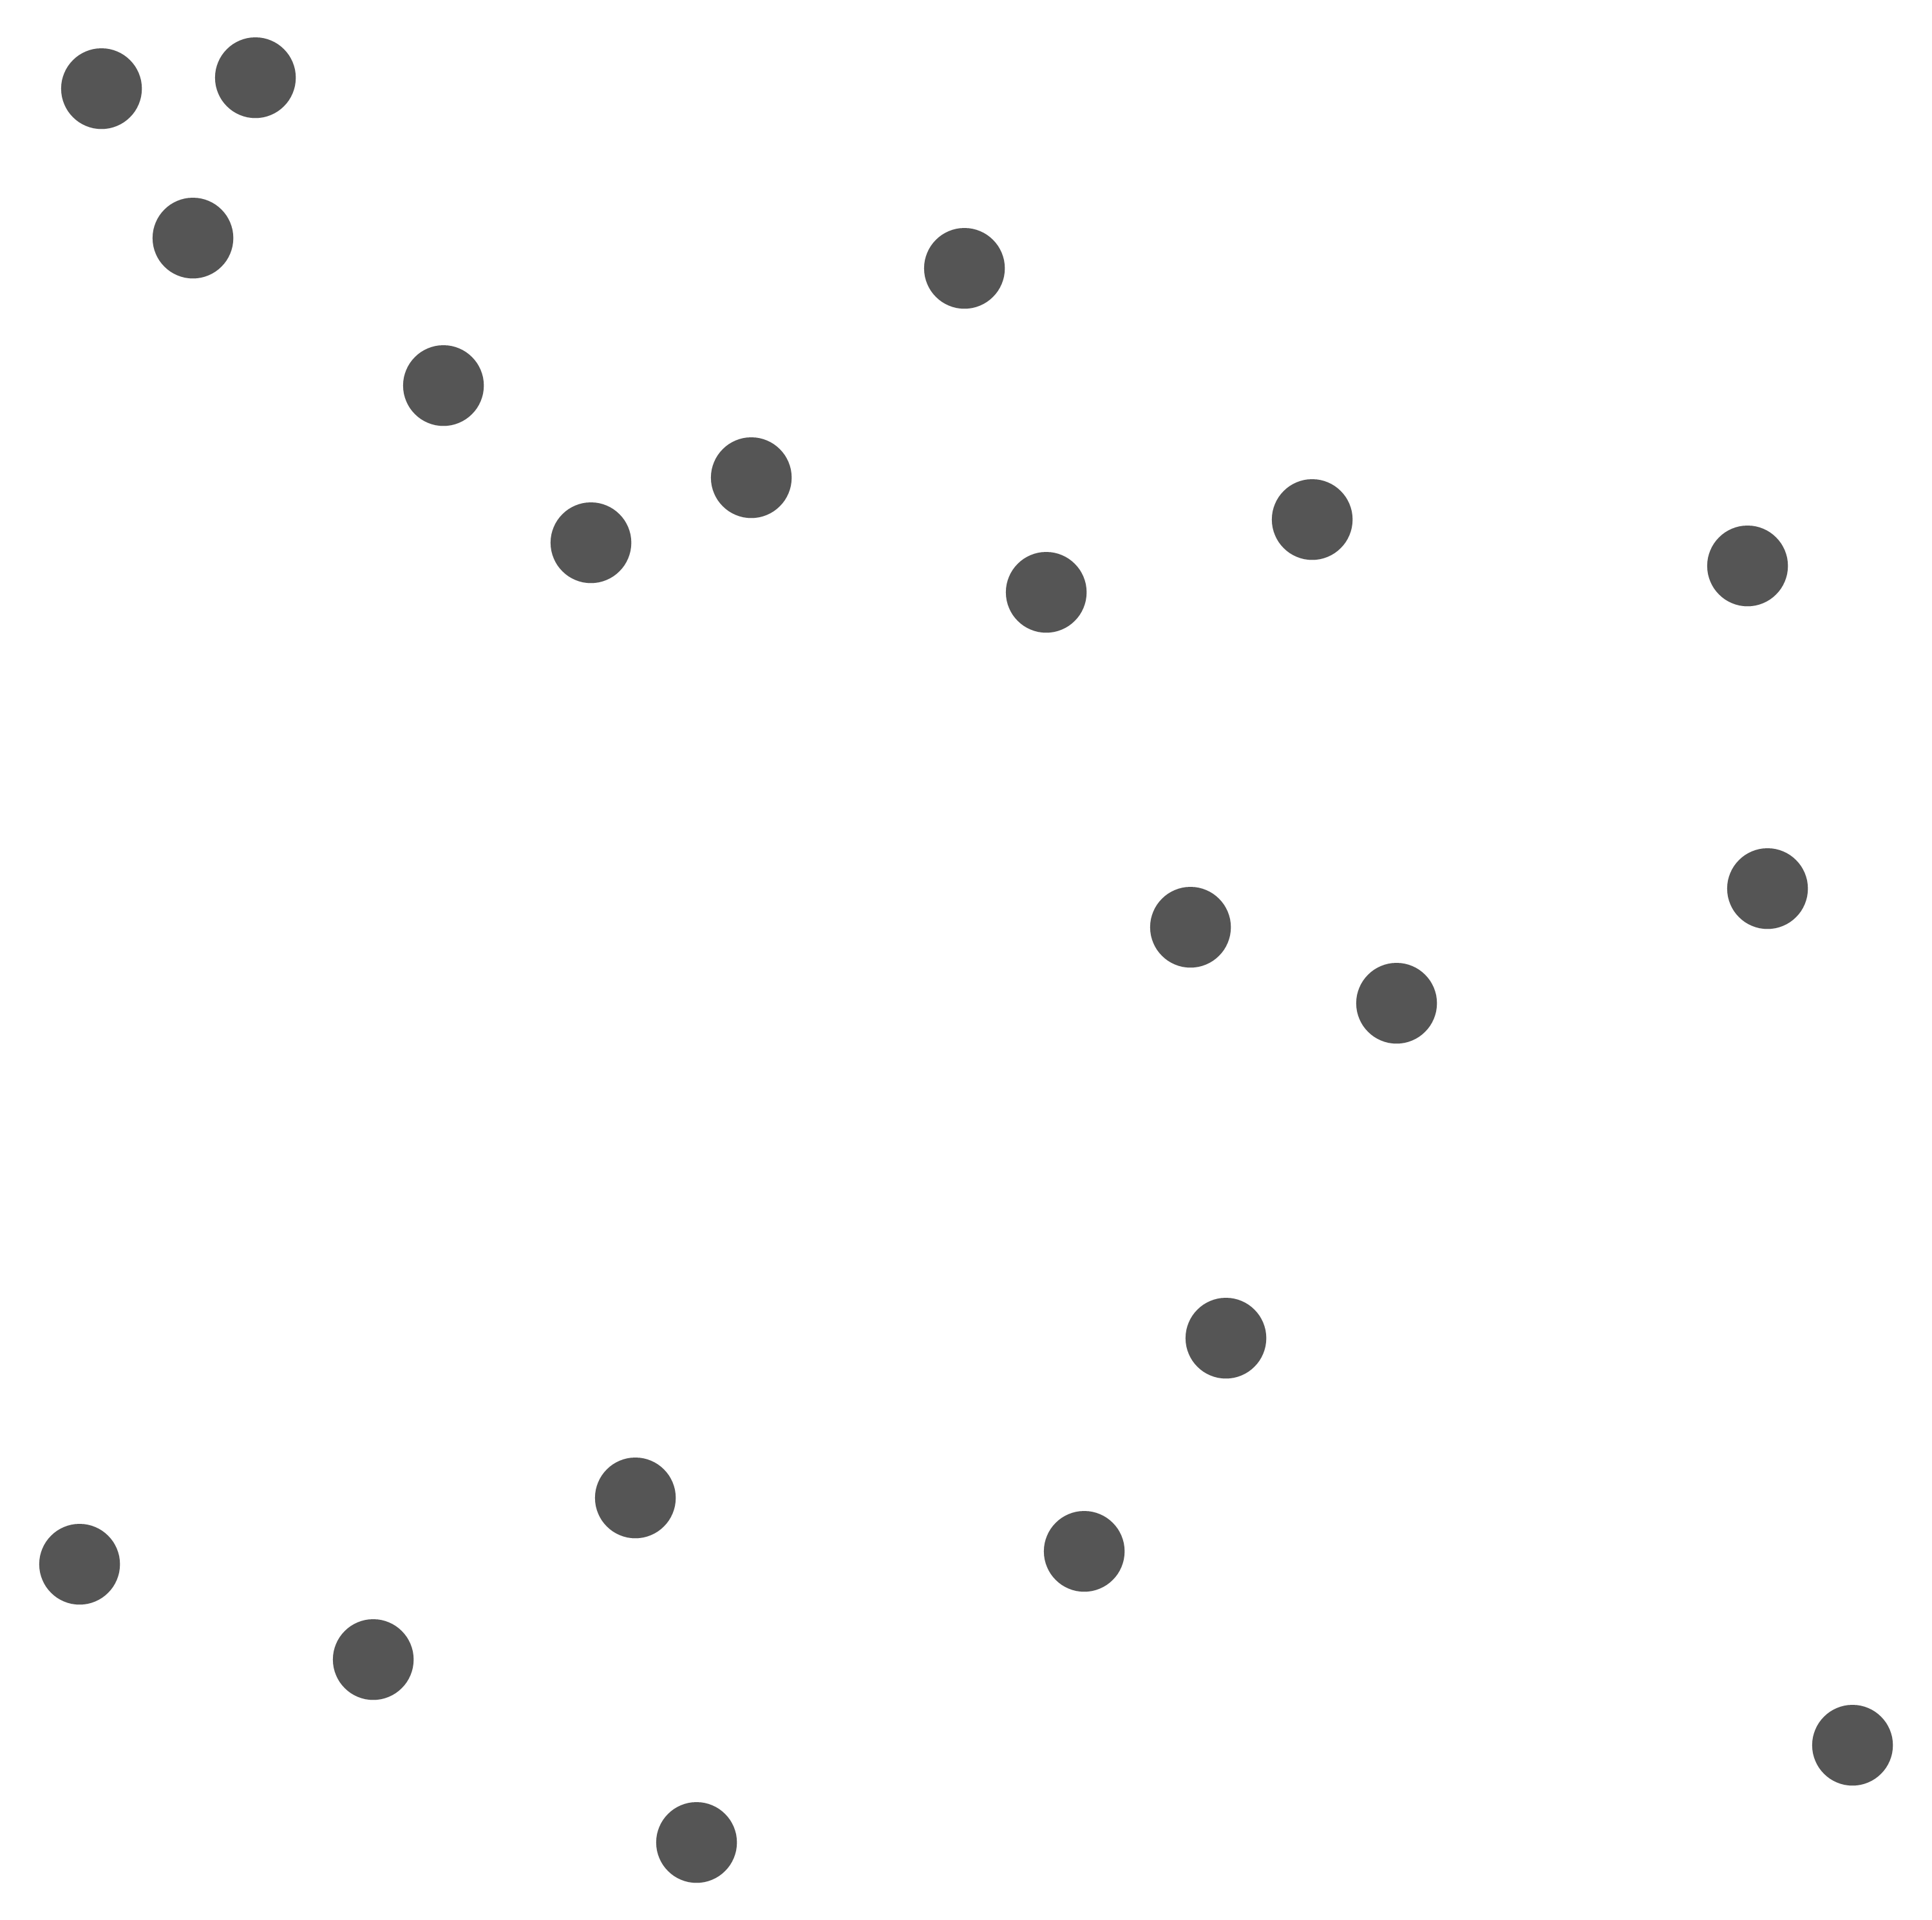
\includegraphics[width=0.23\textwidth]{submissions/Piotr2023/fig/knn1.png}}}%
    \hfill
    \subfloat[$k$-NN graph together with a balanced partition]{{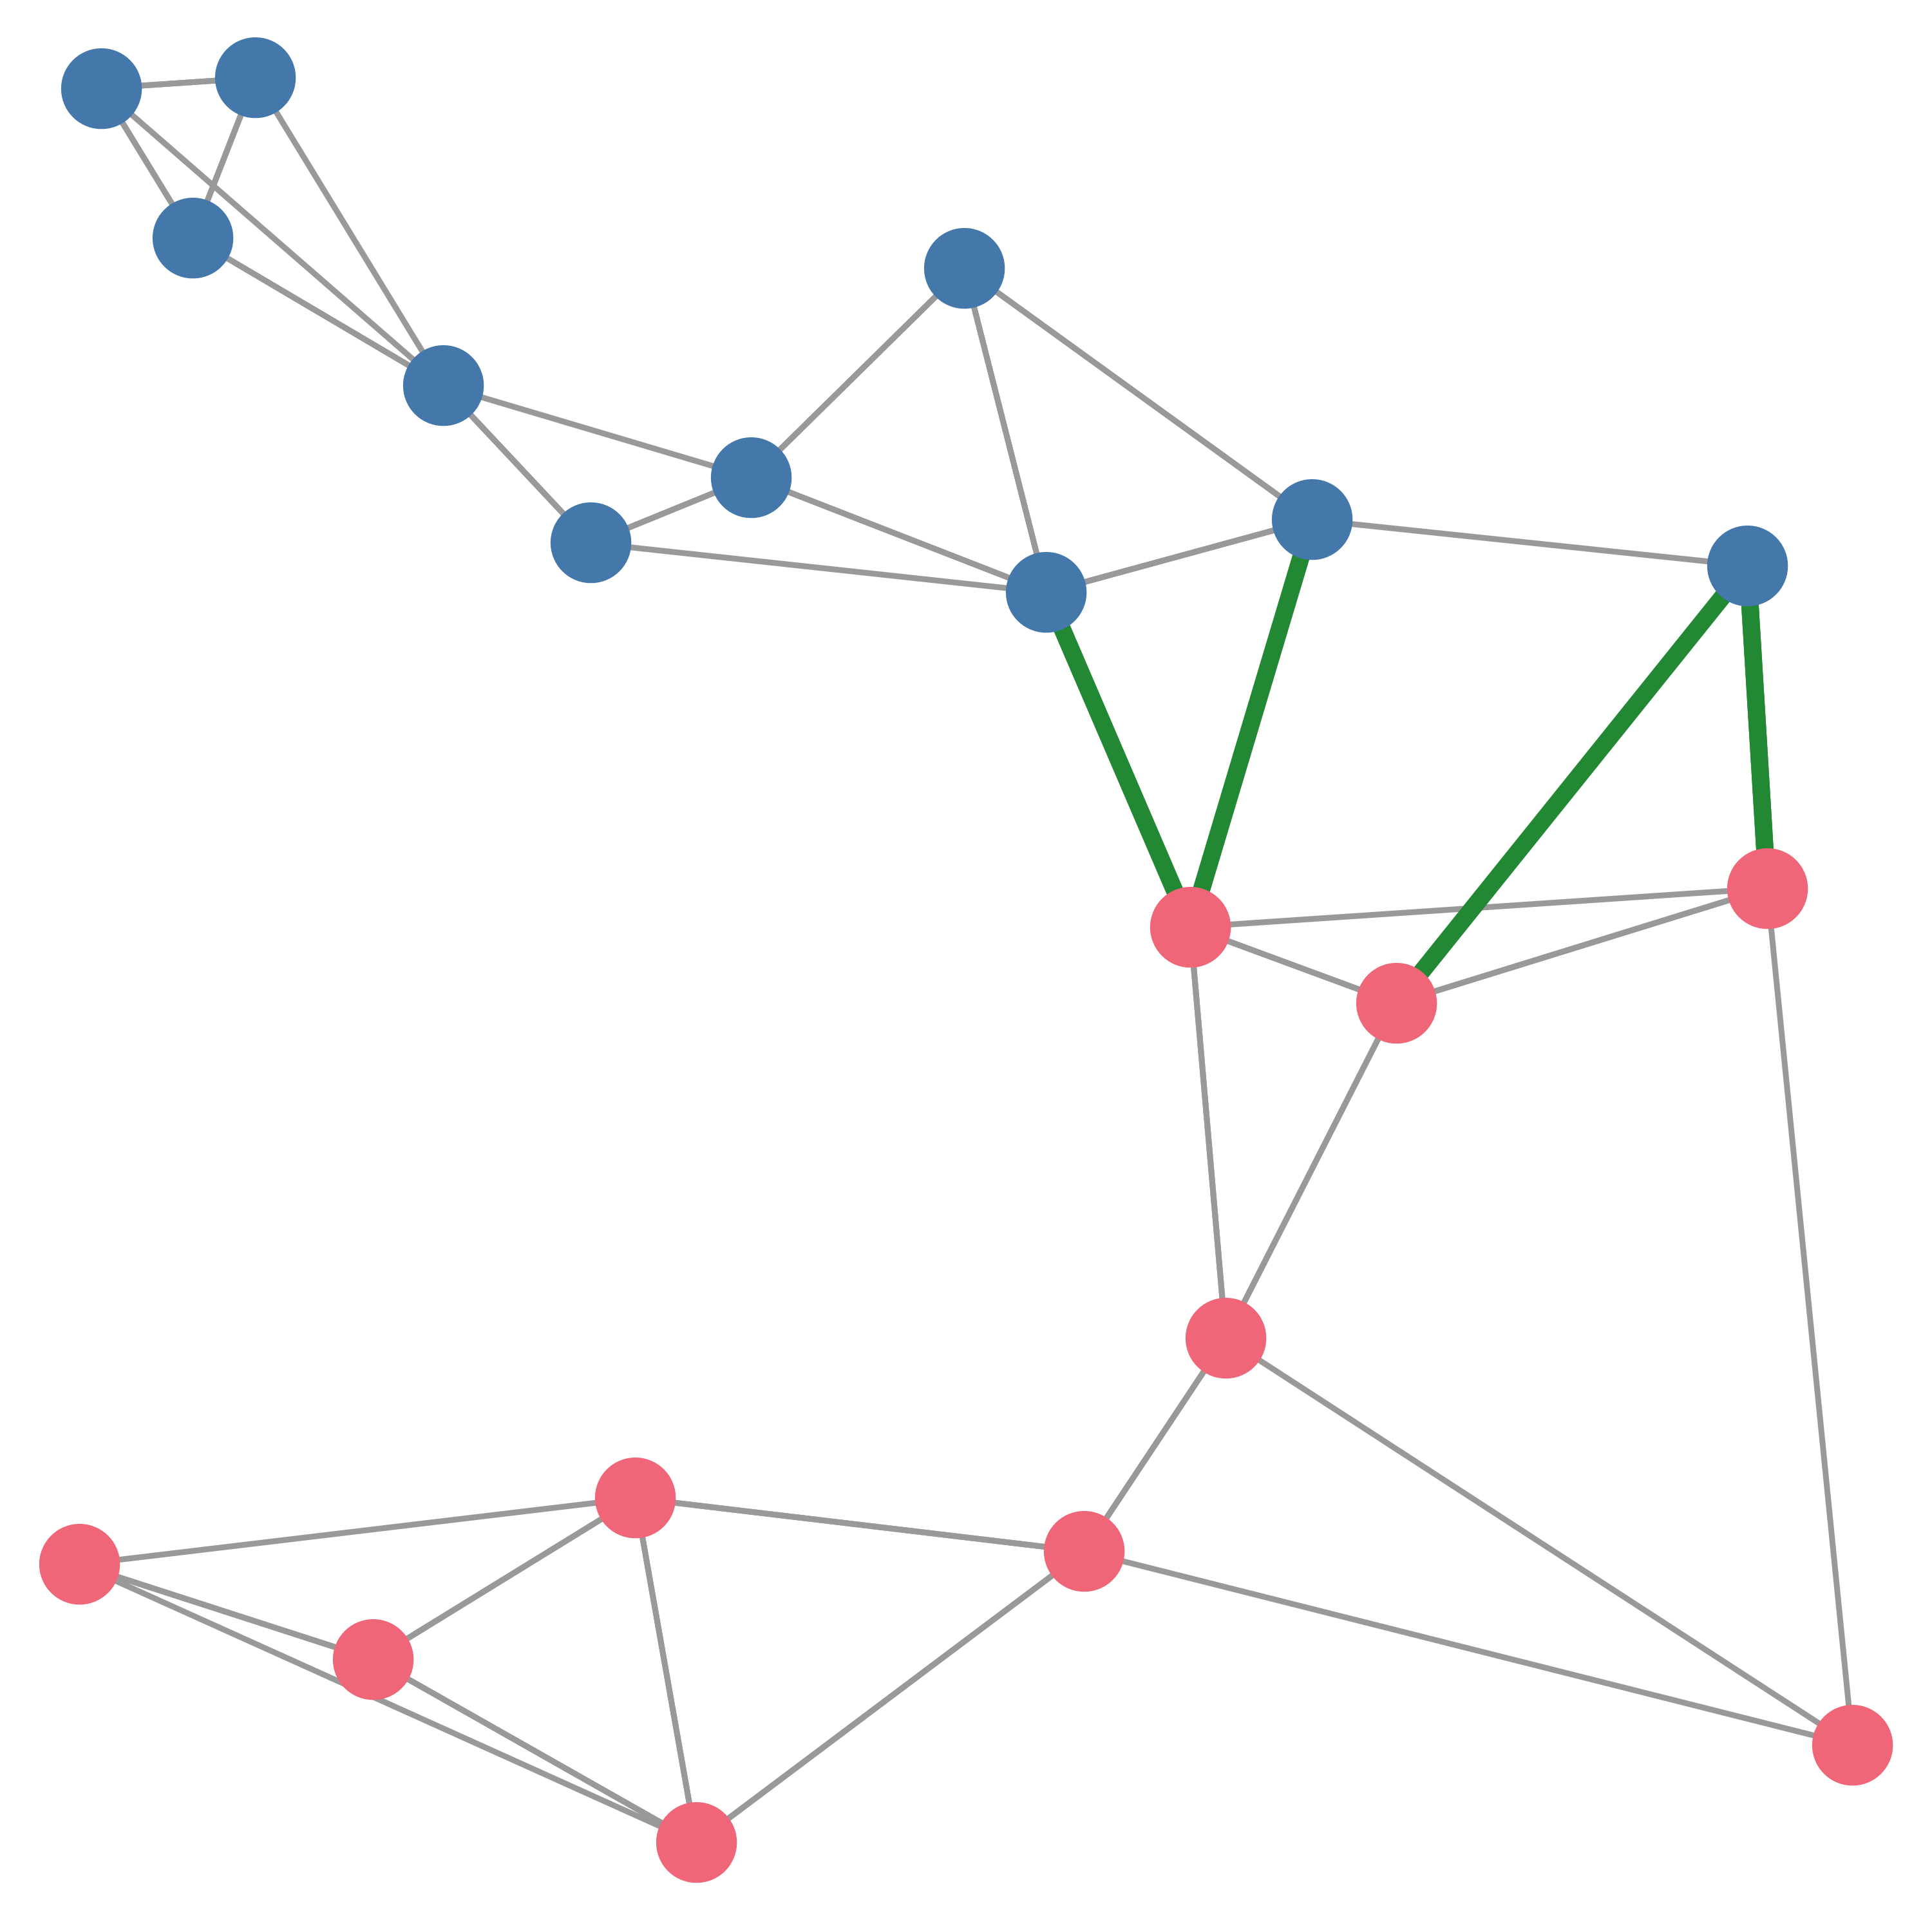
\includegraphics[width=0.23\textwidth]{submissions/Piotr2023/fig/knn2.png}}}%
    \hfill
    \subfloat[Learned partition]{{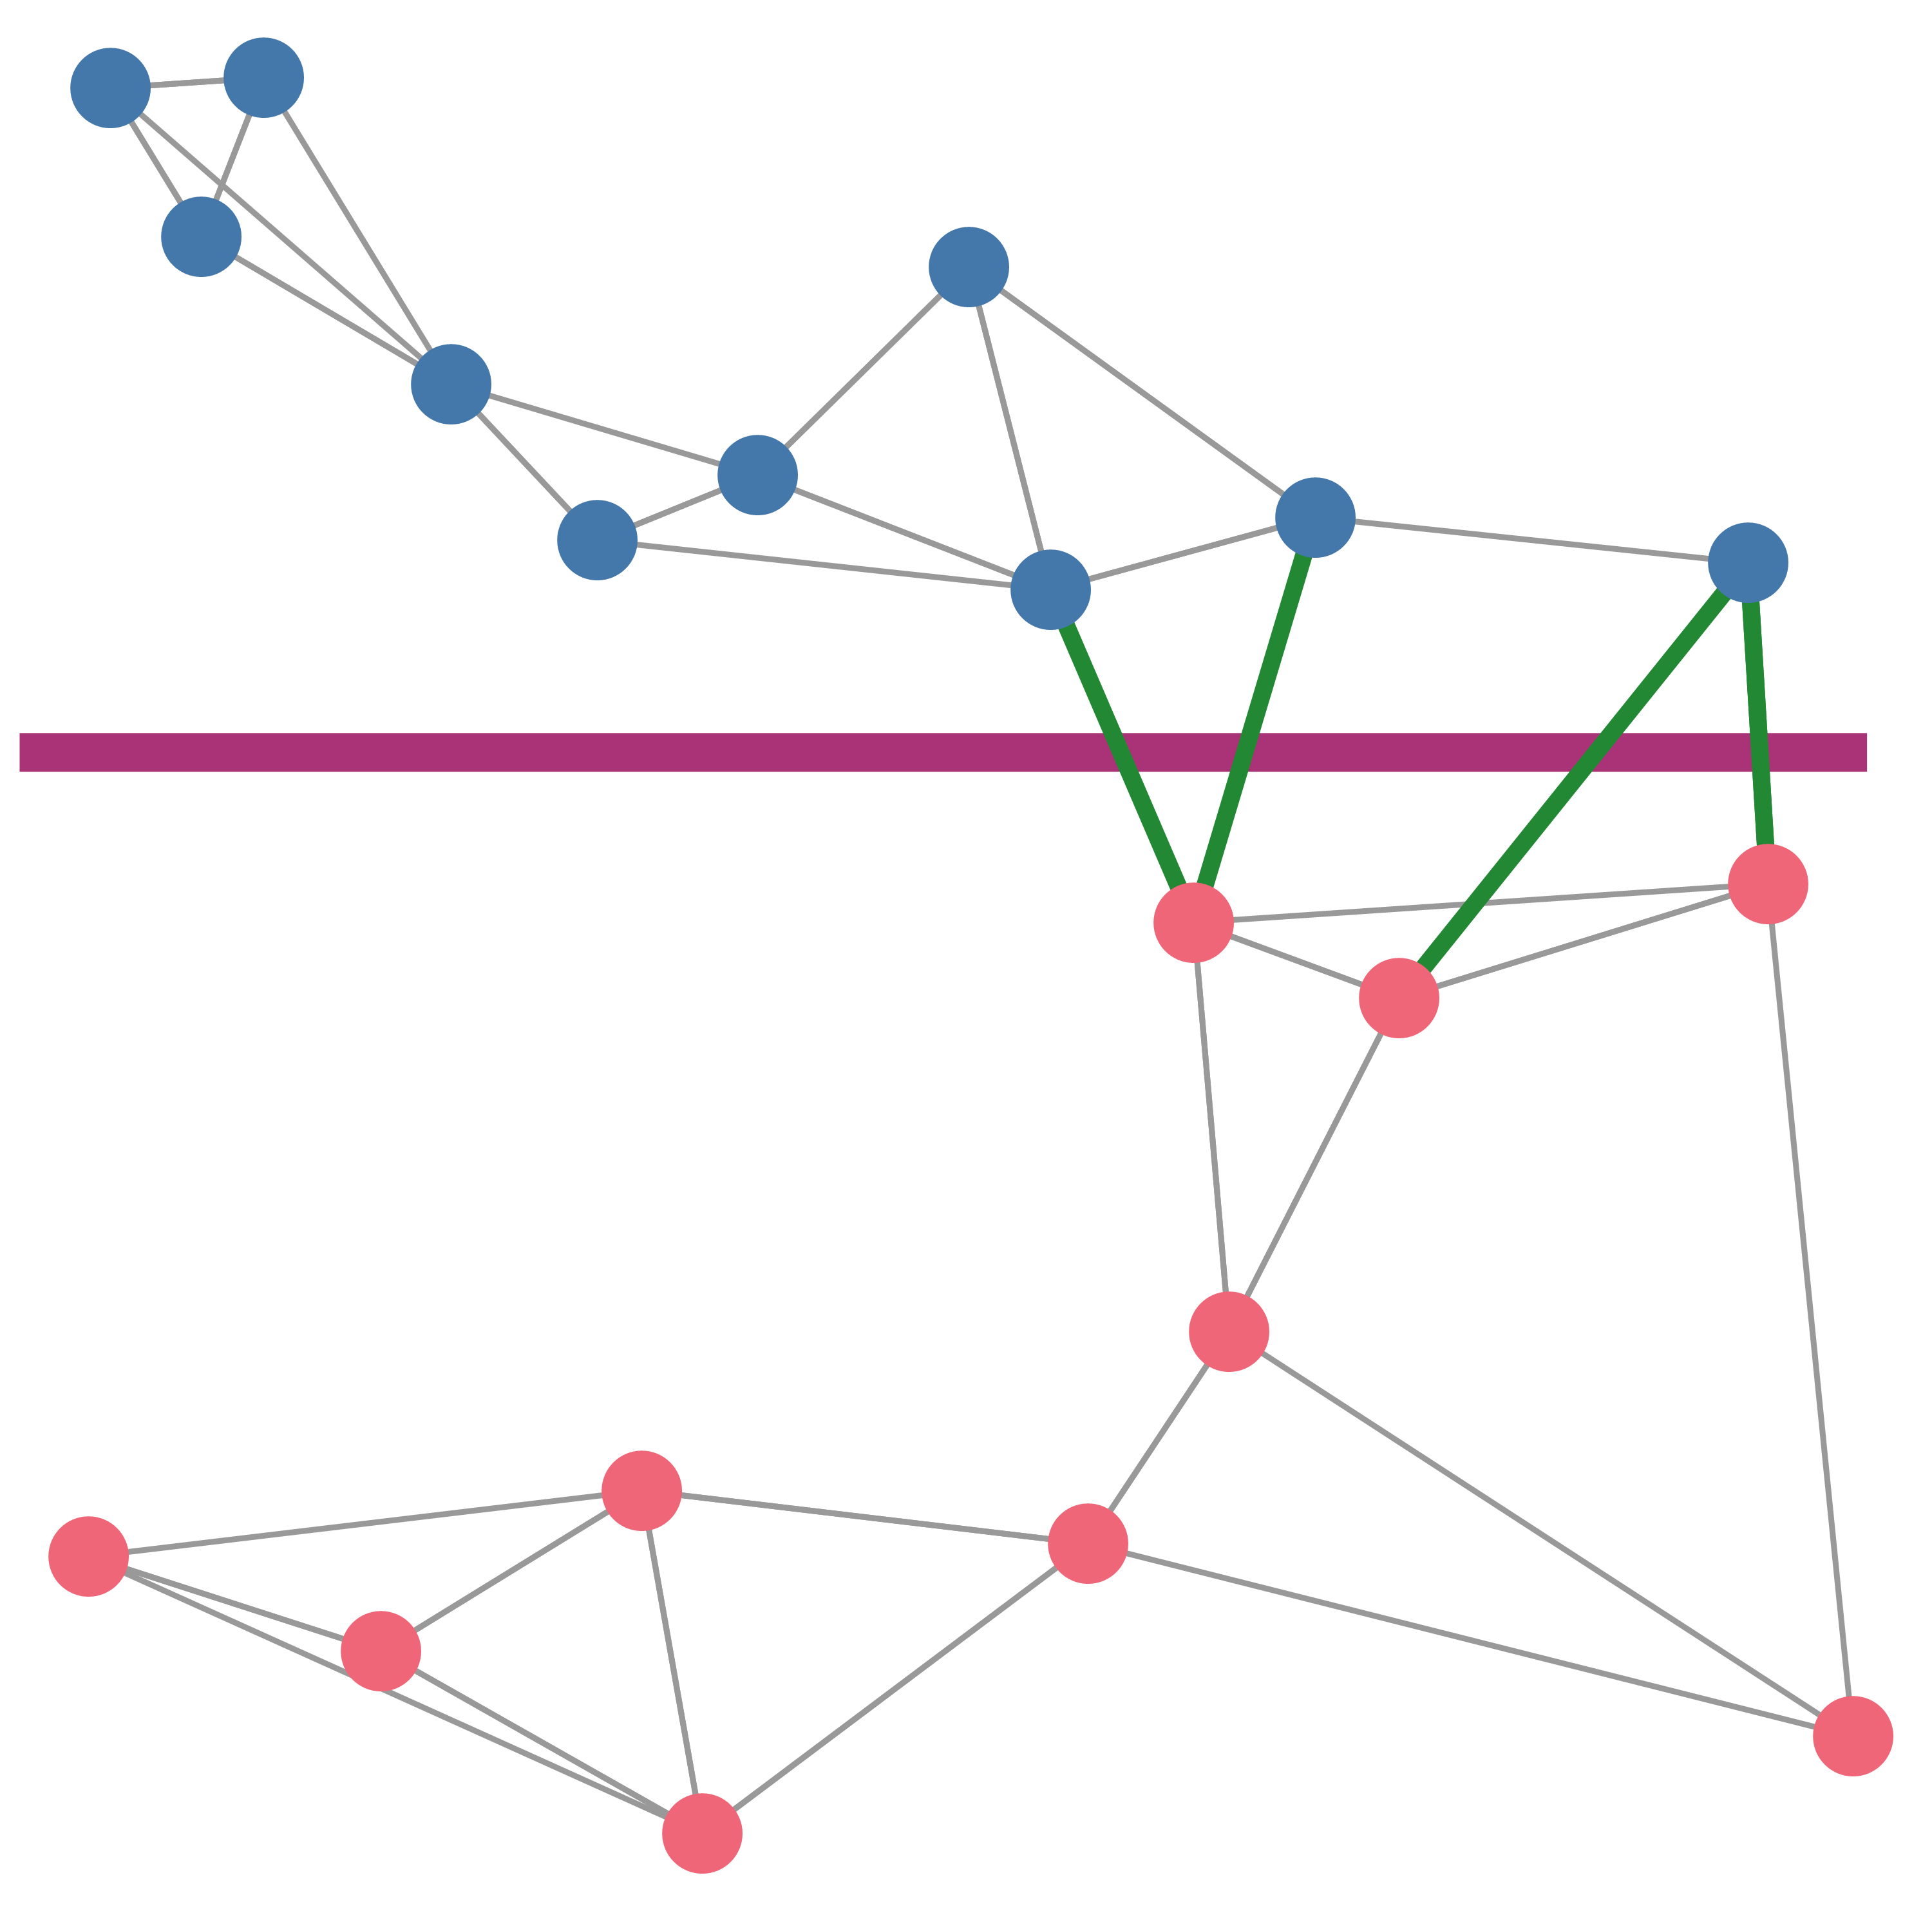
\includegraphics[width=0.23\textwidth]{submissions/Piotr2023/fig/knn3.png}}}%
    \caption{Stages of our framework}
        \label{piotr_fig:pipeline}
\end{figure*}


\section{Our method}

%\paragraph{Training}
Given a dataset $P\subseteq\mathbb{R}^d$ of $n$ points, and a number of bins $m>0$, our goal is to find a partition $\mathcal{R}$ of $\mathbb{R}^d$ into $m$ bins with the following properties:
\begin{CompactEnumerate}
    \item\emph{Balanced:} The number of data points in each bin is not much larger than $n / m$.
    \item\emph{Locality sensitive:} For a typical query point $q \in \mathbb{R}^d$, most of its nearest neighbors belong to the same bin of $\mathcal{R}$. We assume that queries and data points come from similar distributions.
    \item\emph{Simple:} The partition should admit a compact description
    and, moreover, the point location process should be computationally efficient. For example, we might look for a space partition induced by hyperplanes.
\end{CompactEnumerate}

Formally, we want the partition $\mathcal{R}$ that minimizes the loss $E_q\left[\sum_{p\in N_k(q)}\mathbf1_{\mathcal{R}(p)\neq\mathcal{R}(q)}\right]$ s.t.~$\forall_{p\in P}\;|\mathcal{R}(p)|\leq (1+\eta)(n/m)$,
%\[ \E_q\left[\sum_{p\in N_k(q)}\mathbf1_{\mathcal{R}(p)\neq\mathcal{R}(q)}\right] \;\;\;\; s.t. \;\;\;\; \forall_{p\in P}\;|\mathcal{R}(p)|\leq O(m/n) , \]
where $q$ is sampled from the query distribution, $N_k(q)\subset P$ is the set of its $k$ nearest neighbors in $P$, $\eta>0$ is a balance parameter, and $\mathcal{R}(p)$ denotes the part of $\mathcal{R}$ that contains $p$.


First, suppose that the query is chosen as a \emph{uniformly random data point}, $q \sim P$. Let $G$ be the $k$-NN graph of $P$, whose vertices are the data points, and each vertex
is connected to its $k$ nearest neighbors. Then the above problem boils down to partitioning vertices of the graph $G$ into $m$ bins such that each bin contains roughly $n / m$ vertices, and the number of edges crossing between different bins is as small as possible (see Figure~\ref{piotr_fig:pipeline}(b)). This \emph{balanced graph partitioning}
problem is extremely well-studied, and there are available combinatorial partitioning solvers that produce very high-quality solutions.
In our implementation, we use the open-source solver KaHIP~\cite{sandersschulz2013}, which is based on a sophisticated local search.

More generally, we need to handle out-of-sample queries, i.e., which are not contained in $P$.
Let $\widetilde{\mathcal{R}}$ denote the partition of $G$ (equivalently, of the dataset $P$) found by the graph partitioner.
To convert $\widetilde{\mathcal{R}}$ into a solution to our problem, we need to extend it to a partition $\mathcal{R}$ of the whole space $\mathbb{R}^d$ that would work well for query points.
In order to accomplish this, we train a model that, given a query point $q \in \mathbb{R}^d$,
predicts which of the $m$ bins of $\widetilde{\mathcal{R}}$ the point $q$ belongs to (see Figure~\ref{piotr_fig:pipeline}(c)). We use the dataset $P$ as a training set,
and the partition $\widetilde{\mathcal{R}}$ as the labels -- i.e., each data point is labeled with the ID of the bin of $\widetilde{\mathcal{R}}$ containing it. 
The method is summarized in Algorithm~\ref{piotr_alg:main}.
The geometric intuition for this learning step is that -- even though the partition $\widetilde{\mathcal{R}}$ is obtained by combinatorial means, and in principle might consist of ill-behaved subsets of $\mathbb{R}^d$ -- in most practical scenarios, we actually expect it to be close to being induced by a simple partition of the ambient space.
For example, if the dataset
is fairly well-distributed on the unit sphere, %$S^{d-1} \subset \mathbb{R}^d$
and the number of bins is $m = 2$,
a balanced cut of $G$ should be close to a hyperplane.

The choice of model to train depends on the desired properties of the output partition $\mathcal{R}$.
For instance, if we are interested in a hyperplane partition,
we can train a linear model using SVM or regression.  In this paper, we instantiate the learning step with both \emph{linear models}
and \emph{small-sized neural networks.}
Here, there is natural tension between the size of the model we train and the accuracy of the resulting classifier, and hence the quality of the partition we produce.
A larger model yields better NNS accuracy, at the expense of computational efficiency.
We discuss this in Section 3.

\paragraph{Multi-probe querying}
Given a query point $q$, the trained model can be used to assign it to a bin of a partition $\mathcal{R}$, and search for nearest neighbors within the data points in that part.
In order to achieve high search accuracy,
we actually train the model to predict \emph{several} bins for a given query point,
which are likely to contain nearest neighbors.
For neural networks, this can
be done naturally by taking several largest outputs of the last layer.
By searching through more bins (in the order of preference predicted by the model) we can achieve better accuracy, allowing for a trade-off between computational resources and accuracy.


\paragraph{Hierarchical partitions} When the required number of bins $m$ is large, in order to improve the efficiency of the resulting partition,
it pays off to produce it in a hierarchical manner. Namely, we first find a partition of $\mathbb{R}^d$ into $m_1$ bins, then recursively partition each
of the bins into $m_2$ bins, and so on, repeating the partitioning for $L$ levels.
The total number of bins in the overall partition is $m = m_1 \cdot m_2 \cdot \ldots m_L$.
See Figure~\ref{piotr_fig:hierarchical} for illustration.
The advantage of such a hierarchical partition is that it is much simpler to navigate
than a one-shot partition with $m$ bins.

\begin{figure}
    \centering
    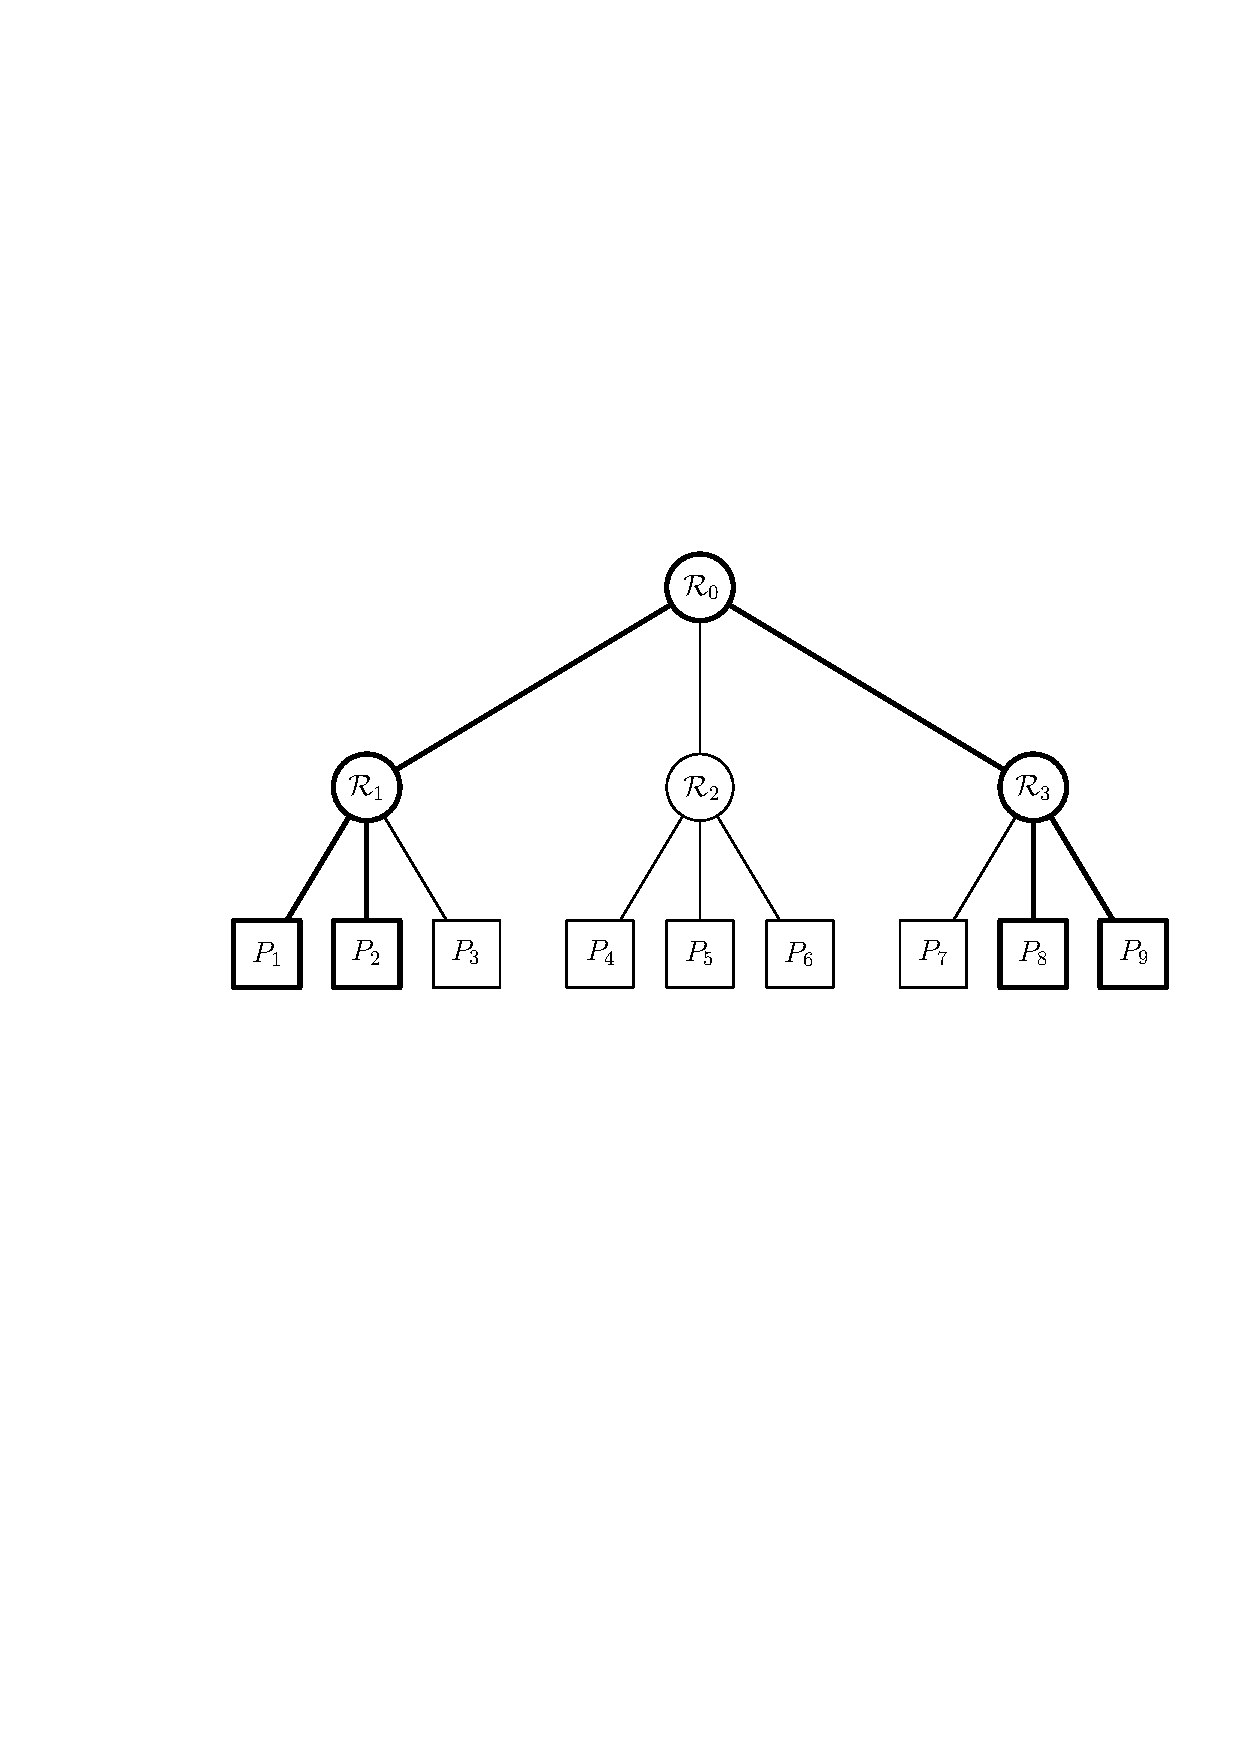
\includegraphics[width=0.47\textwidth]{submissions/Piotr2023/fig/tree.pdf}
    \caption{Hierarchical partition into $9$ bins with $m_1 = m_2 = 3$. $\mathcal{R}_i$'s are partitions,
    $P_j$'s are the bins of the dataset. Multi-probe query procedure, which descends into $2$ bins, may visit the bins marked in bold.}
        \label{piotr_fig:hierarchical}
\end{figure}

\newcommand{\INDENT}{\hspace{1em}}
\begin{algorithm}[!t]
\caption{Nearest neighbor search with a learned space partition}
\label{piotr_alg:main}
%\smallskip{\hrule height.2pt}\smallskip
\smallskip
\textbf{Preprocessing}\\ 
Input: Dataset $P\subset\R^d$, integer parameter $k>0$, number of bins $m>0$
\smallskip{\hrule height.2pt}\smallskip
\smallskip
\begin{algorithmic}[1]
   \STATE Build a $k$-NN graph $G$ of $P$.
   \STATE Run a balanced graph partitioning algorithm on $G$ into $m$ parts. Number the parts arbitrarily as $1,\ldots,m$. Let $\pi(p)\in\{1,\ldots,m\}$ denote the part containing $p$, for every $p\in P$.
   \STATE Train a machine learning model $M$ with training set $P$ and labels $\{\pi(p)\}_{p\in P}$. For every $x\in\R^d$, let $M(x)\in\{1,\ldots,m\}$ denote the prediction of $M$ on $x$.
\smallskip
\end{algorithmic}
\smallskip
$M(\cdot)$ defines our $m$-way partition of $\R^d$. Note that it is possible that $\pi(p)\neq M(p)$ for some $p\in P$, if $M$ attains imperfect training accuracy.
\smallskip{\hrule height.2pt}\smallskip
\smallskip
\textbf{Query}\\ 
Input: query point $q\in\R^d$, number of bins to search $b$
\smallskip{\hrule height.2pt}\smallskip
\smallskip
\begin{algorithmic}[1]
   \STATE Run inference on $M$ to compute $M(q)$.
   \STATE Search for a near neighbor of $q$ in the bin $M(q)$, i.e., among the candidates $\{p\in P:M(p)=M(q)\}$.
   \STATE If $M$ furthermore predicts a~\emph{distribution} over bins, search for a near neighbor in the $b$ top-ranked bins according to the ranking induced by the distribution (i.e., from the most likely bin to less likely ones).
\smallskip
\end{algorithmic}
\end{algorithm}

%\subsection{Neural LSH}
\paragraph{Neural LSH with soft labels}
In the primary instantiation of our framework, we set the supervised learning component to a a neural network with a small number of layers and constrained hidden dimensions (the exact parameters are specified in the next section).
%In one instantiation of the supervised learning component, we use neural networks with a small number of layers and constrained hidden dimensions. The exact parameters are specified in the next section.
%The exact parameters depend on the size of the training set, and are specified in the next section.
%
%The depths of the networks and the hidden dimension are intentionally constrained, to reduce overfitting, memory usage, and training time.
%
%\irnote{Soft labels!}
%
%\paragraph{Soft labels}
In order to support effective multi-probe querying, we need to infer not just the bin that contains the query point, but rather a \emph{distribution} over bins that are likely to contain this point and its neighbors.
A $T$-probe candidate list is then formed from all data points in the $T$ most likely bins.
%
In order to accomplish this, we use~\emph{soft labels} for data points generated as follows. For $S \geq 1$ and a data point $p$, the soft label
$\mathcal{P} = (p_1, p_2, \ldots, p_m)$ is a distribution over the bin containing a point chosen uniformly at random among $S$ nearest neighbors of $p$ (including $p$ itself).
Now, for a predicted distribution $\mathcal{Q}=(q_1, q_2,\ldots,q_m)$, we seek to minimize the KL divergence between $\mathcal{P}$ and $\mathcal{Q}$:
$\sum_{i=1}^m p_i \log \frac{p_i}{q_i}$.
Intuitively, soft labels help guide the neural network with information about multiple bin ranking. $S$ is a hyperparameter that needs to be tuned; we study its setting in the appendix (cf.~Figure~\ref{piotr_fig:hyper_plots_s}).
%Section~\ref{piotr_sec:additional_experiments}.
%We study its setting in Section~\ref{piotr_sec:additional_experiments}.

%The purpose of the soft labels is to guide the neural network with information about the ranking of bins for searching nearest neighbors. Optimizing w.r.t.~$\mathcal{P}$ allows the model to predict multiple bins more accurately, which is necessary for achieving high accuracy via multi-probe querying.
%
%$S$ is a hyperparameter that needs to be tuned. In practice, the accuracy in the objective function increases in the regime where $S$ is larger than $k$, as more neighbors give the network a more ``complete'' distribution over bins.

\section{Sparse hyperplane-induced cuts in $k$-NN graphs}

We state and prove a theorem that shows, under certain mild assumptions, that the $k$-NN graph of a dataset $P \subseteq \Rbb^d$ can be partitioned
by a hyperplane such that the induced cut is sparse (i.e., has few crossing edges while the sizes of two parts are similar).
The theorem is based on the framework of~\cite{andoni2018data,andoni2018holder}
and uses spectral techniques.

We start with some notation.
Let $N_k(p)$ be the set of $k$ nearest neighbors of $p$ in $P$.
The degree of $p$ in the $k$-NN graph is $\deg(p) = |N_k(p)\cup\{p' \in P \mid p \in N_k(p')\}|$.
Let $\mathcal{D}$ be the distribution over the dataset $P$, where a point $p \in P$ is sampled with probability proportional to its degree $\deg(p)$.
Let $\mathcal{D}_{\mathrm{close}}$ be the distribution over pairs $(p, p') \in P \times P$,
where $p \in P$ is uniformly random, and $p'$ is a uniformly random element of $N_k(p)$. 
%(the set of $k$ nearest neighbors of $p$).
Denote $\alpha = \mathrm{E}_{(p, p') \in \mathcal{D}_{\mathrm{close}}}[\|p - p'\|_2^2]$
and $\beta = \mathrm{E}_{x_1 \sim \mathcal{D}, x_2 \sim \mathcal{D}}[\|p_1 - p_2\|_2^2]$.
We will proceed assuming that $\alpha$ (typical distance between a data point and its
nearest neighbors) is noticeably smaller than $\beta$ (typical distance between two
independent data points).

The following theorem implies, informally speaking, that if
$\alpha \ll \beta$, then there exists a hyperplane
which splits the dataset into two parts of not too different size
while separating only few pairs of $(p, p')$, where $p'$ is
one of the $k$ nearest neighbors of $p$.
For the proof of the theorem, see \cite{arxiv}.

\begin{theorem}
\label{piotr_spectral_thm}
There exists a hyperplane $H = \{x \in \Rbb^d \mid \langle a, x\rangle = b\}$ such that the following holds.
Let $P = P_1 \cup P_2$ be the partition of $P$ induced by $H$: $P_1 = \{p \in P \mid \langle a, p \rangle \leq b\}$,
$P_2 = \{p \in P \mid \langle a, p \rangle > b\}$. Then, one has:
\begin{equation}
\label{piotr_eqeqeq3}
\frac{\mathrm{Pr}_{(p, p') \sim \mathcal{D}_{\mathrm{close}}}[\mbox{$p$ and $p'$ are separated by $H$}]}{\min\{\mathrm{Pr}_{p \sim \mathcal{D}}[p \in P_1],\mathrm{Pr}_{p \sim \mathcal{D}}[p \in P_2]\}} \leq \sqrt{\frac{2 \alpha}{\beta}}.
\end{equation}
\end{theorem}


\section{Experiments}\label{piotr_sec:experiments}

\paragraph{Datasets}
For the experimental evaluation, we use three standard ANN benchmarks~\cite{aumuller2017ann}: SIFT (image descriptors, 1M 128-dimensional points), GloVe (word embeddings~\cite{pennington2014glove}, approximately 1.2M 100-dimensional points, normalized), and MNIST (images of digits, 60K 784-dimensional points).
All three datasets come with $10\,000$ query points, which are used for evaluation. 
We include the results for SIFT and GloVe in the main text, and MNIST in \cite{arxiv}.

\paragraph{Evaluation metrics}
We mainly investigate the trade-off between the number of candidates generated for a query point, and the $k$-NN accuracy, defined as the fraction of its $k$ nearest neighbors that are among those candidates.
The number of candidates determines the processing time of an individual query.
Over the entire query set, we report both the \emph{average}
as well as the \emph{$0.95$-th quantile} of the number of candidates.
The former measures the \emph{throughput}\footnote{Number of queries per second.} of the data structure, while the latter measures its \emph{latency.}\footnote{Maximum time per query, modulo a small fraction of outliers.}
We focus on parameter regimes that yield $k$-NN accuracy of at least $0.75$, in the setting $k=10$.
Additional results with broader regimes of accuracy and of $k$ are included in the appendix.
%We mostly focus on parameter regimes that lead to $k$-NN accuracy of at least $0.8$.
%The experiments in this section use $k = 10$; see appendix for other values of $k$.

\paragraph{Our methods}
We evaluate two variants of our method, with two different choices of the supervised learning component:% in our framework.

\begin{CompactItemize}
\item\textbf{Neural LSH:}
In this variant we use small neural networks.
%Their exact architecture is detailed in the next section.
%We compare Neural LSH to partitions obtained by $k$-means clustering. As mentioned in Section 1, this method produces high quality partitions, and the other methods we evaluate (LSH and
%and Iterative Quantization) do not match it.
We compare this method with $k$-means clustering, Iterative Quantization (ITQ)~\cite{gong2013iterative}, Cross-polytope LSH~\cite{andoni2015practical}, and Neural Catalyzer~\cite{sablayrolles2018spreading} composed over $k$-means clustering.
We evaluate partitions into $16$ bins and $256$ bins. 
We test both one-level (non-hierarchical) and two-level (hierarchical) partitions.
Queries are multi-probe.

\item\textbf{Regression LSH:} This variant uses logistic regression as the supervised learning component
and, as a result, produces very simple partitions induced by \emph{hyperplanes.}
We compare this method with PCA trees~\cite{sproull1991refinements,kumar2008good,abdullah2014spectral}, random projection trees~\cite{dasgupta2013randomized}, and recursive bisections using $2$-means clustering.
We build trees of hierarchical bisections of depth up to $10$ (thus total number of leaves up to $1024$).
The query procedure descends a single root-to-leaf path and returns the candidates in that leaf.
\end{CompactItemize}

\subsection{Implementation details}

Neural LSH uses a fixed neural network architecture for the top-level partition,
and a fixed architecture for all second-level partitions.
Both architectures consist of several blocks, where each block is a fully-connected layer + batch normalization~\cite{ioffe2015batch} + ReLU activations.
The final block is followed by a fully-connected layer and a softmax layer.
The resulting network predicts a distribution over the bins of the partition.
%
The only difference between the top-level network the second-level network architecture is their number of blocks ($b$) and the size of their hidden layers ($s$).
In the top-level network we use $b=3$ and $s=512$.
In the second-level networks we use $b=2$ and $s=390$.
%
%The only differences between the two architectures are the number of blocks and the sizes of hidden layers: for the top-level partition, we have three blocks and the hidden layers are of size $512$, while for the second-level partitions, one has two blocks, and the size of the hidden layers is $390$.
%
To reduce overfitting, we use dropout with probability $0.1$ during training.
The networks are trained using the Adam optimizer \cite{adam2015} for under $20$ epochs on both levels. We reduce the learning rate multiplicatively at regular intervals. The weights are initialized with Glorot initialization~\cite{glorot2010}.
To tune soft labels, we try different values of $S$ between $1$ and $120$.

We evaluate two settings for the number of bins in each level, $m=16$ and $m=256$ (leading to a total number of bins of the total number of bins in the two-level experiments are $16^2=256$ and $256^2 = 65\,536$, respectively).
In the two-level setting with $m=256$ the bottom level of Neural LSH uses $k$-means instead of a neural network, to avoid overfitting when the number of points per bin is tiny. The other configurations (two-levels with $m=16$ and one-level with either $m=16$ or $m=256$) we use Neural LSH at all levels.

We slightly modify the KaHIP partitioner to make it more efficient on the $k$-NN graphs. Namely, we introduce a hard threshold
of $2000$ on the number of iterations for the local search part of the algorithm, which speeds up the partitioning dramatically,
while barely affecting the quality of the resulting partitions.

%\irnote{Compress it.} A hierarchical partition produces a tree in which each node corresponds to a partition into $m$ bins. In our experiments, we evaluate $m=16$ and $m=256$, thus the total number of bins in the two-level experiments are $16^2=256$ and $256^2 = 65\,536$ respectively. In the latter case, each bin contains fewer than $20$ data points, which is too small for supervised learning without overfitting. Therefore, in the two-level experiment with $m=256$, we use Neural LSH at the top-level and $k$-means clustering at the bottom level. In the other experiments (two-levels with $m=16$ and one-level with $m\in\{16,256\}$) we use Neural LSH at all levels.

%\irnote{This paragraph can go.} Note that multiple partitions of $\mathbb{R}^d$ can be combined in ways other than the hierarchical approach we evaluate.
%For example, the common technique Product Quantization combines multiple invocations of $k$-means in a Cartesian product fashion, over a decomposition of $\mathbb{R}^d$ into orthogonal subspaces~\cite{jegou2011product,babenko2012inverted}.
%There are various techniques to tune and improve this approach~\cite{norouzi2013cartesian,ge2014optimized,wu2017multiscale}.
%Since the focus of our paper is to compare the quality of individual partitions, we use hierarchical partitioning as a baseline approach to combining partitions.
%Nonetheless, we note that the above Cartesian product approach and related ideas can be readily applied to Neural LSH as well.

%multiple partitions of $\mathbb{R}^d$ can be combined in ways other than the hierarchical approach we evaluate.
%For example, Product Quantization
%uses partitioning vectors into blocks~\cite{jegou2011product,babenko2012inverted}, which was improved further in~\cite{norouzi2013cartesian,ge2014optimized}.
%Since the focus of this paper is to compare quality of individual partitions, we choose the hierarchical
%approach as the simplest and perhaps the cleanest. Note that the block partitioning and related ideas
%can be readily applied to Neural LSH as well.


%when $10$-NN accuracy varies from $0.85$ and higher.
%\irnote{Should we report the preprocessing times?}
%\ynote{We decided not to.}
%\twnote{Then I am commenting this out!}

\subsection{Comparison with multi-bin methods}\label{piotr_sec:kmeanscomparison}
Figure~\ref{piotr_fig:kmeans_plots} shows the empirical comparison of Neural LSH with $k$-means clustering, ITQ, Cross-polytope LSH, and Neural Catalyzer composed over $k$-means clustering.
It turns out that $k$-means is the strongest among these baselines.\footnote{It is important to note that ITQ is not designed to produce space partitions; as explained in Section 1, it does so as a side-effect. Simiarly, Neural Catalyzer is not designed to enhance partitions. The comparison is intended to show that they do not outperform indexing techniques despite being outside their intended application.} 
% We evaluate these methods outside their intended application.}
The points depicted in Figure~\ref{piotr_fig:kmeans_plots} are those that attain accuracy $\geq0.75$. In~\cite{arxiv} we include the full accuracy range for all methods.

%However, if one wishes to use partitions to split points across machines to build a distributed NNS data structure, then a
%single-level settings seems to be more suitable.

In all settings considered, 
Neural LSH yields consistently better partitions than $k$-means.\footnote{We note that two-level partitioning with $m=256$ is the best performing configuration of $k$-means, for both SIFT and GloVe, in terms of the minimum number of candidates that attains $0.9$ accuracy. Thus we evaluate this baseline at its optimal performance.} Depending on the setting, $k$-means requires significantly more candidates to achieve the same accuracy:
\begin{CompactItemize}
    \item Up to $117\%$ more for the average number of candidates for GloVe;
    \item Up to $130\%$ more for the $0.95$-quantiles of candidates for GloVe;
    \item Up to $18\%$ more for the average number of candidates for SIFT;
    \item Up to $34\%$ more for the $0.95$-quantiles of candidates for SIFT;
\end{CompactItemize}
Figure~\ref{piotr_table_kmeans} lists the largest multiplicative advantage in the number of candidates of Neural LSH compared to $k$-means, for accuracy values of at least $0.85$.
Specifically, for every configuration of $k$-means, we compute the ratio between the number of candidates in that configuration and the number of candidates of Neural LSH in its optimal configuration, among those that attained at least the same accuracy as that $k$-means configuration.


\begin{figure*}
\centering
\begin{tabular}{|r|r|cc|cc|}
\hline
 && \textbf{GloVe} &  & \textbf{SIFT} & \\
 && Averages & $0.95$-quantiles  & Averages & $0.95$-quantiles \\
 \hline
\textbf{One level} & $16$ bins & 1.745 & 2.125 & 1.031 & 1.240 \\
& $256$ bins & 1.491 & 1.752 & 1.047 & 1.348 \\
\hline
\textbf{Two levels} & $16$ bins & 2.176 & 2.308 & 1.113 & 1.306 \\
& $256$ bins & 1.241 & 1.154 & 1.182 & 1.192 \\
\hline
\end{tabular}
\caption{Largest ratio between the number of candidates for Neural LSH and $k$-means over the settings where both attain the same target $10$-NN accuracy, over accuracies of at least $0.85$.
%for which Neural LSH obtains no worse accuracy than $k$-means.
See details in Section~\ref{piotr_sec:kmeanscomparison}.}
\label{piotr_table_kmeans}
\end{figure*}

We also note that in all settings except two-level partitioning with $m=256$,\footnote{As mentioned earlier, in this setting Neural LSH uses $k$-means at the second level, due to the large overall number of bins compared to the size of the datasets. This explains why the gap between the average and the $0.95$-quantile number of candidates of Neural LSH is larger for this setting.}
Neural LSH produces partitions for which the 
$0.95$-quantiles for the number of candidates are very close to the average number of candidates, which indicates very little variance between query times over different query points.
In contrast, the respective gap in the partitions produced by $k$-means is much larger, since unlike Neural LSH, it does not directly favor balanced partitions.
This implies that Neural LSH might be particularly suitable for latency-critical
NNS applications.

%We also note that for all the settings except ``two levels, $256$ bins on each'' (where we use $k$-means for the second level) Neural LSH finds partitions, for which the $0.95$-quantiles for the number of candidates are very close to the average number of candidates, however for the $k$-means the respective gap is significant. This disparity leads to the gap between $k$-means and Neural LSH significantly increasing when one passes from averages to the $0.95$-quantiles. Hence, Neural LSH might be particularly suitable for latency-critical NNS applications.

\begin{figure*}%
    \centering
    \subfloat[GloVe, one level, $16$ bins]{{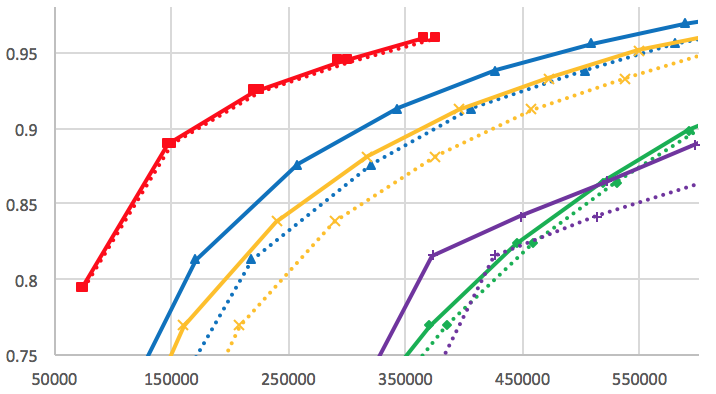
\includegraphics[width=0.50\textwidth]{submissions/Piotr2023/fig/nlsh_glove_1_16}}}%
    \subfloat[SIFT, one level, $16$ bins]{{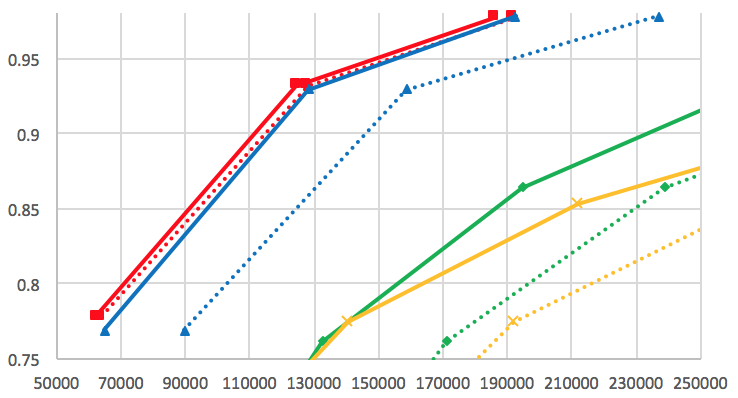
\includegraphics[width=0.50\textwidth]{submissions/Piotr2023/fig/nlsh_sift_1_16}}}%

    \subfloat[GloVe, one level, $256$ bins]{{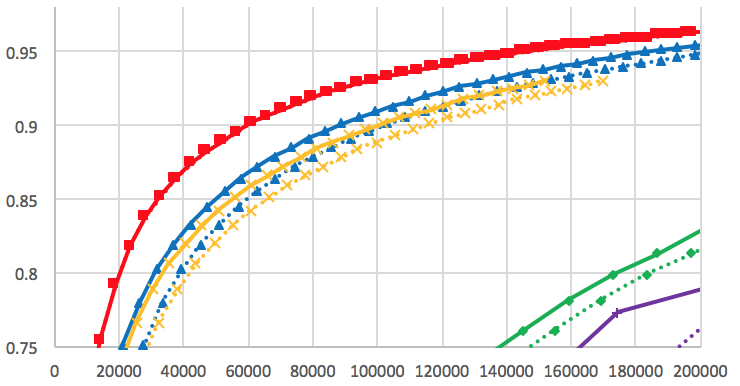
\includegraphics[width=0.50\textwidth]{submissions/Piotr2023/fig/nlsh_glove_1_256}}}%
    \subfloat[SIFT, one level, $256$ bins]{{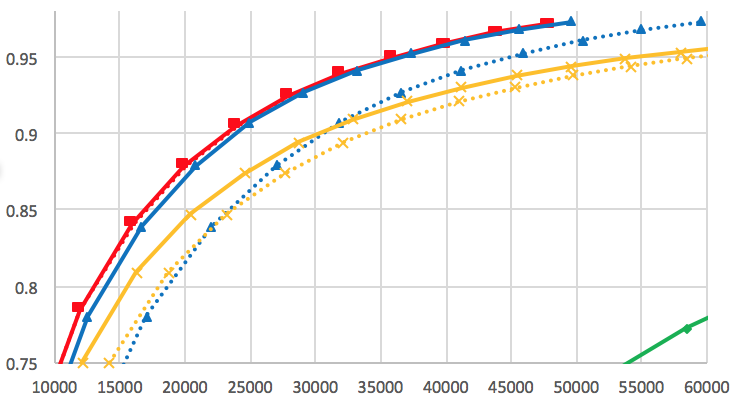
\includegraphics[width=0.50\textwidth]{submissions/Piotr2023/fig/nlsh_sift_1_256}}}%
    
    \subfloat[GloVe, two levels, $16$ bins]{{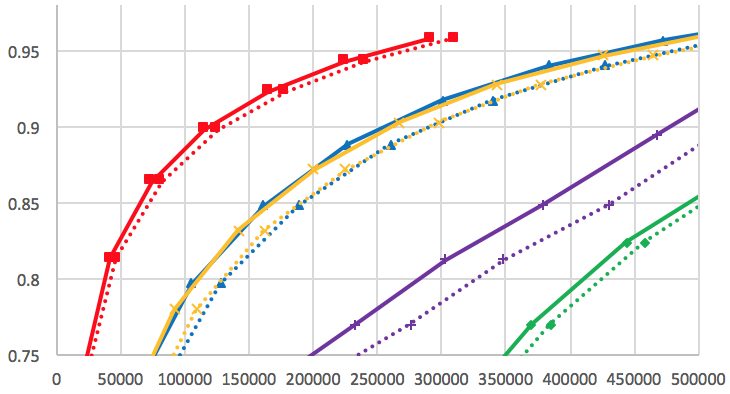
\includegraphics[width=0.50\textwidth]{submissions/Piotr2023/fig/nlsh_glove_2_16}}}%
    \subfloat[SIFT, two levels, $16$ bins]{{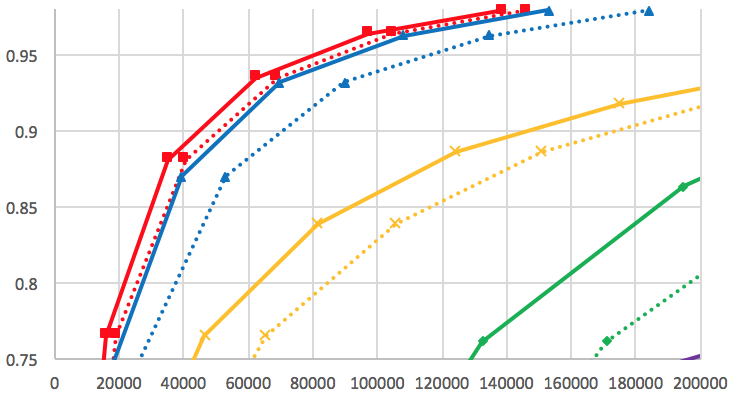
\includegraphics[width=0.50\textwidth]{submissions/Piotr2023/fig/nlsh_sift_2_16}}}%

    \subfloat[GloVe, two levels, $256$ bins, $k$-means at 2nd level]{{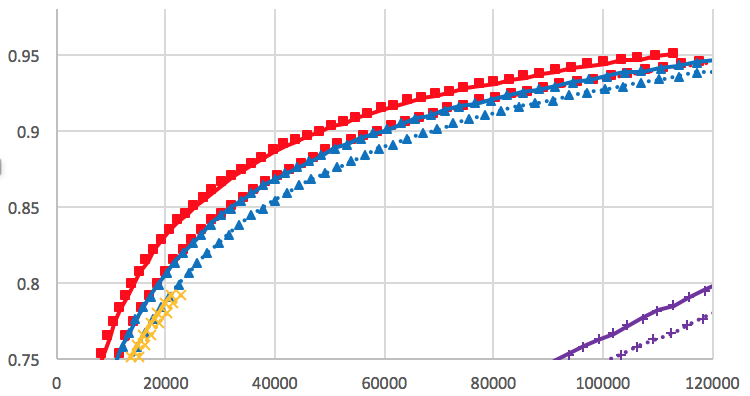
\includegraphics[width=0.50\textwidth]{submissions/Piotr2023/fig/nlsh_glove_2_256}}}%
    \subfloat[SIFT, two levels, $256$ bins, $k$-means at 2nd level]{{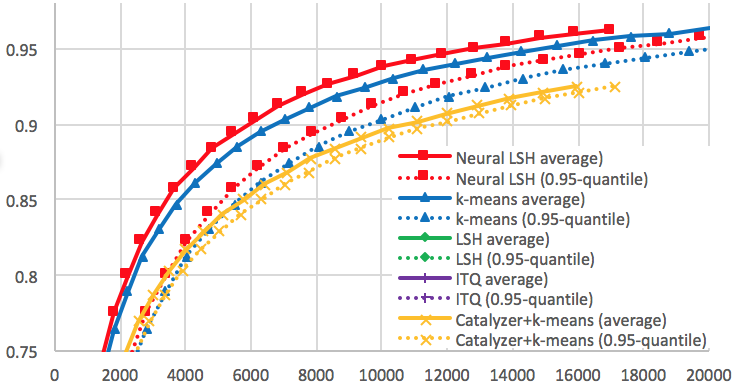
\includegraphics[width=0.50\textwidth]{submissions/Piotr2023/fig/nlsh_sift_2_256}}}%
    \caption{Comparison of Neural LSH with baselines; x-axis is the number of candidates, y-axis is the $10$-NN accuracy}%
    \label{piotr_fig:kmeans_plots}
\end{figure*}


\paragraph{Model sizes.}
The largest model size learned by Neural LSH is equivalent to storing about $\approx 5700$ points for SIFT, or $\approx 7100$ points for GloVe.%\footnote{The difference accounts for the different network architecture used for them, as well as their different dimensionality.}
This is considerably larger than $k$-means with $k\leq256$, which stores at most $256$ points.
Nonetheless, we believe the larger model size is acceptable for Neural LSH, for the following reasons.
%\begin{itemize}
    %\item
    First, in most of the NNS applications, especially for the distributed setting, the bottleneck in the high accuracy regime is the memory accesses needed to retrieve candidates and the further processing (such as distance computations, exact or approximate). The model size is not a hindrance as long as does not exceed certain reasonable limits (e.g., it should fit into a CPU cache).
    Neural LSH significantly reduces the memory access cost, while increasing the model size by an acceptable amount.
    %\item
    Second, we have observed that the quality of the Neural LSH partitions is not too sensitive to decreasing the sizes
    the hidden layers. The model sizes we report are, for the sake of concreteness, the largest ones that still lead to improved performance. Larger models do not increase the accuracy, and sometimes decrease it due to overfitting.
%\end{itemize}



\subsection{Comparison with tree-based methods}

Next we compare binary decision trees, where in each tree node a \emph{hyperplane} is used to determine which of the two subtrees to descend into. We generate hyperplanes with the following methods: Regression LSH, the Learned KD-tree of~\cite{cayton2008learning}, the Boosted Search Forest of~\cite{li2011learning}, cutting the dataset into two equal halves along the top PCA direction~\cite{sproull1991refinements,kumar2008good},
$2$-means clustering, and random projections of the centered dataset~\cite{dasgupta2013randomized,keivani2018improved}.
We build trees of depth up to $10$, which correspond to hierarchical partitions with the up to $2^{10} = 1024$ bins. Results for GloVe and SIFT are summarized in Figure~\ref{piotr_fig:trees_results} (see appendix).
For random projections, we run each configuration $30$ times and average the results.

For GloVe, Regression LSH significantly outperforms $2$-means,
while for SIFT, Regression LSH essentially matches $2$-means in terms of the \emph{average} number of candidates,
but shows a noticeable advantage in terms of the $0.95$-percentiles.
In both instances, Regression LSH significantly outperforms PCA tree, and all of the above methods
dramatically improve upon random projections.

Note, however, that random projections have an additional benefit: in order to boost search
accuracy, one can simply repeat the sampling process several times and generate an ensemble of
decision trees instead of a single tree. This allows making each individual tree relatively deep,
which decreases the overall number of candidates, trading space for query time. Other considered approaches (Regression LSH, $2$-means, PCA tree) are inherently deterministic, and boosting their accuracy requires more care:
for instance, one can use partitioning into blocks as in~\cite{jegou2011product}, or alternative approaches like~\cite{keivani2018improved}. Since we focus
on individual partitions and not ensembles, we leave this issue out of the scope.

\begin{figure*}%
    \centering
    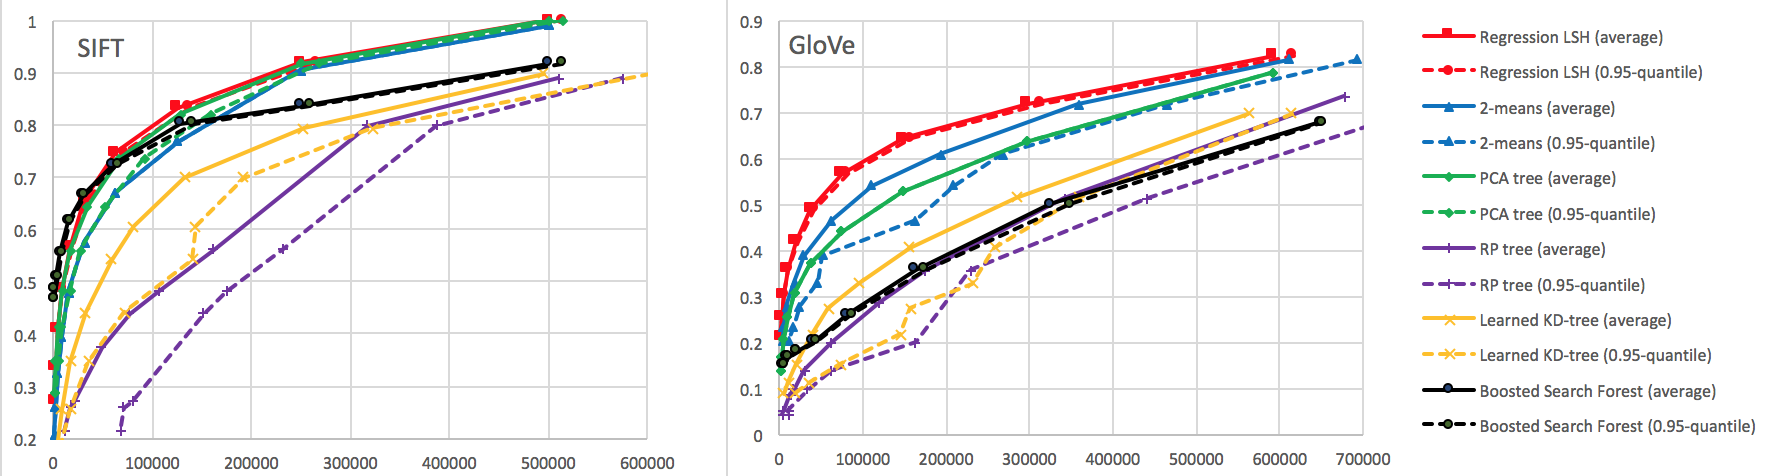
\includegraphics[width=\textwidth]{submissions/Piotr2023/fig/plot_trees.png}

    \caption{Comparison of decision trees built from hyperplanes: x-axis -- number of candidates, y-axis -- $10$-NN accuracy}%
    \label{piotr_fig:trees_results}
\end{figure*}

%\subsection{Additional experiments}\label{piotr_sec:additional_experiments}
%\paragraph{Additional experiments.}
%In the appendix we inlclude several additional experiments: \emph{(i)} We evaluate the $50$-NN accuracy of Neural LSH when the partitioning step is run on either the $10$-NN or the $50$-NN graph.\footnote{Neural LSH can solve $k$-NNS by partitioning the $k'$-NN graph, for any $k,k'$; they do not have to be equal.}
%Both settings outperform $k$-means, and the gap
%between using the $10$-NN and $50$-NN graphs is negligible,
%which indicates the robustness of Neural LSH.
%\emph{(ii)} We study the effect of tuning the size of soft labels $S$.
%We show that setting $S$ to be at least $15$ is immensely beneficial
%compared to $S = 1$, but beyond that we start observing diminishing returns.

\subsection{Additional experiments}
In this section we include several additional experiments.

First, we study the effect of setting $k$.
We evaluate the $50$-NN accuracy of Neural LSH when the partitioning step is run on either the $10$-NN or the $50$-NN graph.\footnote{Neural LSH can solve $k$-NNS by partitioning the $k'$-NN graph, for any $k,k'$; they do not have to be equal.} We compare both algorithms to $k$-means with $k = 50$. 
Figure~\ref{piotr_fig:hyper_plots_k} compares these three algorithms on
GloVe for $16$ bins reporting
average numbers of candidates. From this plot,
we can see that for $k = 50$, Neural LSH
convincingly outperforms $k$-means,
and whether we use $10$-NN or $50$-NN graph matters very little.

Second, we study the effect of varying $S$ (the soft labels parameter) for Neural LSH on GloVe for $256$ bins.
See Figure~\ref{piotr_fig:hyper_plots_s} where we report the average number of candidates. As we can see from the plot,
the setting $S = 15$ yields much better results
compared to the vanilla case of $S = 1$. However,
increasing $S$ beyond $15$ brings diminishing returns  on the overall
accuracy.



\begin{figure*}%
    \centering
    \subfloat[\label{piotr_fig:hyper_plots_k}GloVe, one level, $16$ bins, $50$-NN accuracy using $10$-NN and $50$-NN graphs]{{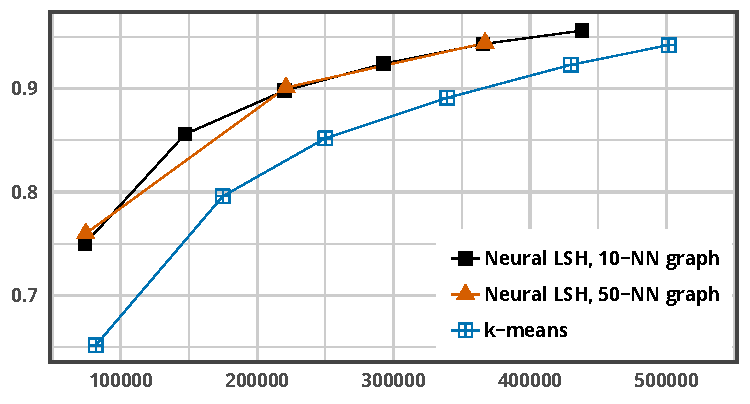
\includegraphics[width=0.50\textwidth]{submissions/Piotr2023/fig/k_plot.pdf}}}%
    \subfloat[\label{piotr_fig:hyper_plots_s}GloVe, one level, $256$ bins, varying $S$]{{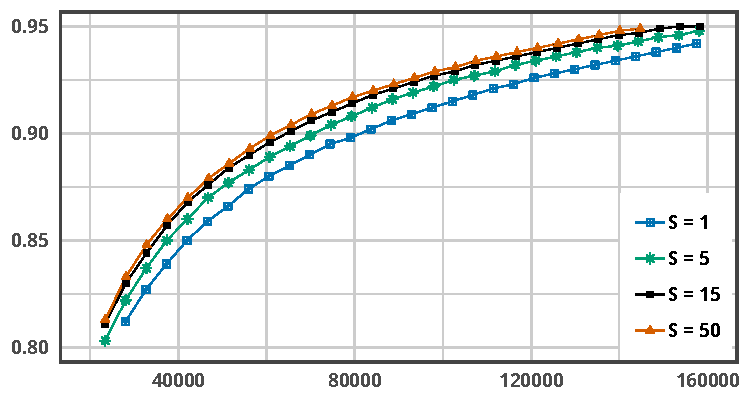
\includegraphics[width=0.50\textwidth]{submissions/Piotr2023/fig/s_plot.pdf}}}%
    \caption{Effect of various hyperparameters}
    \label{piotr_fig:hyper_plots}
\end{figure*}




\section{Conclusions and future directions}

%In this paper, 
We presented a new technique for finding partitions of $\mathbb{R}^d$ which support high-performance indexing for sublinear-time NNS.
It proceeds in two major steps:
%\begin{CompactItemize}
%    \item We start with combinatorial balanced partitioning of the $k$-NN graph of the dataset;
%    \item We extend the resulting partition to the whole ambient space $\mathbb{R}^d$ by using
%    supervised classification (such as logistic regression, neural networks, etc.).
%\end{CompactItemize}
%
(1) We perform a combinatorial balanced partitioning of the $k$-NN graph of the dataset;
(2) We extend the resulting partition to the whole ambient space $\mathbb{R}^d$ by using
    supervised classification (such as logistic regression, neural networks, etc.).
Our experiments show that the new approach consistently outperforms quantization-based and tree-based
partitions.

Our work leads to multiple exciting open problems. Perhaps the most important one is whether it is possible to design a variant of Neural LSH that has {\em provable correctness guarantees}, without sacrificing the empirical performance. Such guarantees could take multiple forms:
\begin{enumerate}
\item {\em approximate nearest neighbor:} the data structure guarantees that, given a query $q$, it returns a point $p'$ whose distance to $q$ is at most some factor $c>1$ greater than the distance from $q$ to its true nearest neighbor.
\item {\em probabilistic near neighbor:} for a given scale parameter $r$ and probability parameter $\delta>0$, given a query $q$, each point $p$ within a distance $r$ from $q$ is returned with probability $1-\delta$.
\end{enumerate}

Algorithms based on locality-sensitive hashing satisfy guarantees (1)~\cite{indyk1998approximate} or (2)~\cite{andoni2005locality}, depending on the implementation. Similarly, some tree-based methods such as~\cite{bawa2005lsh} and \cite{dasgupta2013randomized} satisfy such guarantees. It is thus plausible that one could achieve SOTA empirical performance while guaranteeing some form of correctness. At the same time, we expect this challenge to be somewhat difficult, as the current state-of-the-art indexing algorithms typically lack correctness guarantees. For example,~\cite{haike2023} has recently demonstrated that there exist data sets for which graph-based algorithms such as HNSW~\cite{malkov2018efficient}, NSG~\cite{fu2019fast} or DiskANN~\cite{jayaram2019diskann} must scan a large percentage of data point to return a reasonable approximate nearest neighbor.  
Nevertheless, an initial progress towards this goal has been already made in~\cite{andoni2022learning}.

\iffalse
There is a number of exciting open problems we would like to highlight:

\begin{CompactItemize}
    \item Can we use our approach for NNS over \emph{non-Euclidean} geometries,
    such as the edit distance~\cite{zhang2017embedjoin} or the optimal transport
    distance~\cite{kusner2015word}?
    The graph partitioning step directly carries through,
    but the learning step may need to be adjusted.
    \item Can we jointly optimize a graph partition \emph{and} 
    a classifier at the same time?
    By making the two components aware of each other,
    we expect the quality of the resulting partition of $\mathbb{R}^d$ to improve.
    A related approach has been successfully applied in~\cite{li2011learning} for hyperplane tree partitions.
    \item Can our approach be extended to learning \emph{several} high-quality partitions that complement each other?
    Such an ensemble might be useful to trade query time for
    memory usage~\cite{andoni2017optimal}.
    \item Can we use machine learning techniques to improve \emph{graph-based} indexing techniques~\cite{malkov2018efficient} for NNS? 
    (This is in contrast to partition-based indexing, as done in this work).
    \item Our framework is an example of combinatorial tools aiding
    ``continuous'' learning techniques.
    A more open-ended question is whether other problems can benefit from such symbiosis.
\end{CompactItemize}

\fi

%\bibliography{bibfile}
%\itemsep=1pt

%\bibliographystyle{amsalpha}

\bibliographystyle{plainnat}
\begin{thebibliography}{10}
\itemsep=1pt
\begin{small}
\newcommand{\etalchar}[1]{$^{#1}$}
\providecommand{\bysame}{\leavevmode\hbox to3em{\hrulefill}\thinspace}
\providecommand{\MR}{\relax\ifhmode\unskip\space\fi MR }
% \MRhref is called by the amsart/book/proc definition of \MR.
\providecommand{\MRhref}[2]{%
  \href{http://www.ams.org/mathscinet-getitem?mr=#1}{#2}
}
\providecommand{\href}[2]{#2}


\bibitem{abdullah2014spectral}
Amirali Abdullah, Alexandr Andoni, Ravindran Kannan, and Robert Krauthgamer, \emph{Spectral approaches to nearest neighbor search}, arXiv preprint arXiv:1408.0751 (2014).

\bibitem{andoni2022learning}
Alexandr Andoni and Daniel Beaglehole, \emph{Learning to hash robustly, guaranteed}, International Conference on Machine Learning, PMLR, 2022, pp.~599--618.

\bibitem{aumuller2017ann}
Martin Aum{\"u}ller, Erik Bernhardsson, and Alexander Faithfull, \emph{Ann-benchmarks: A benchmarking tool for approximate nearest neighbor algorithms}, International Conference on Similarity Search and Applications, Springer, 2017, pp.~34--49.

\bibitem{andoni2005locality}
Alexandr Andoni, Mayur Datar, Nicole Immorlica, Piotr Indyk, and Vahab Mirrokni, \emph{Locality-sensitive hashing using stable distributions}, Nearest-Neighbor Methods in Learning and Vision (2005), 61--72.

\bibitem{andoni2008near}
Alexandr Andoni and Piotr Indyk, \emph{Near-optimal hashing algorithms for approximate nearest neighbor in high dimensions}, Communications of the ACM \textbf{51} (2008), no.~1, 117--122.

\bibitem{andoni2015practical}
Alexandr Andoni, Piotr Indyk, Thijs Laarhoven, Ilya Razenshteyn, and Ludwig Schmidt, \emph{Practical and optimal lsh for angular distance}, Advances in Neural Information Processing Systems, 2015, pp.~1225--1233.

\bibitem{andoni2018approximate}
Alexandr Andoni, Piotr Indyk, and Ilya Razenshteyn, \emph{Approximate nearest neighbor search in high dimensions}, arXiv preprint arXiv:1806.09823 (2018).

\bibitem{andoni2018data}
Alexandr Andoni, Assaf Naor, Aleksandar Nikolov, Ilya Razenshteyn, and Erik Waingarten, \emph{Data-dependent hashing via nonlinear spectral gaps}, Proceedings of the 50th Annual ACM SIGACT Symposium on Theory of Computing (2018), 787--800.

\bibitem{andoni2018holder}
\bysame, \emph{H{\"o}lder homeomorphisms and approximate nearest neighbors}, 2018 IEEE 59th Annual Symposium on Foundations of Computer Science (FOCS), IEEE, 2018, pp.~159--169.

\bibitem{bawa2005lsh}
Mayank Bawa, Tyson Condie, and Prasanna Ganesan, \emph{Lsh forest: self-tuning indexes for similarity search}, Proceedings of the 14th international conference on World Wide Web, ACM, 2005, pp.~651--660.

\bibitem{balcan2018learning}
Maria-Florina Balcan, Travis Dick, Tuomas Sandholm, and Ellen Vitercik, \emph{Learning to branch}, International Conference on Machine Learning, 2018.

\bibitem{bahmani2012efficient}
Bahman Bahmani, Ashish Goel, and Rajendra Shinde, \emph{Efficient distributed locality sensitive hashing}, Proceedings of the 21st ACM international conference on Information and knowledge management, ACM, 2012, pp.~2174--2178.

\bibitem{bora2017compressed}
Ashish Bora, Ajil Jalal, Eric Price, and Alexandros~G Dimakis, \emph{Compressed sensing using generative models}, International Conference on Machine Learning, 2017, pp.~537--546.

\bibitem{babenko2012inverted}
Artem Babenko and Victor Lempitsky, \emph{The inverted multi-index}, Computer Vision and Pattern Recognition (CVPR), 2012 IEEE Conference on, IEEE, 2012, pp.~3069--3076.


\bibitem{bhaskara2018distributed}
Aditya Bhaskara and Maheshakya Wijewardena, \emph{Distributed clustering via lsh based data partitioning}, International Conference on Machine Learning, 2018, pp.~569--578.

\bibitem{chen2019sanns}
Hao Chen, Ilaria Chillotti, Yihe Dong, Oxana Poburinnaya, Ilya Razenshteyn, and M~Sadegh Riazi, \emph{Sanns: Scaling up secure approximate k-nearest neighbors search}, arXiv preprint arXiv:1904.02033 (2019).

\bibitem{cayton2008learning}
Lawrence Cayton and Sanjoy Dasgupta, \emph{A learning framework for nearest neighbor search}, Advances in Neural Information Processing Systems, 2007, pp.~233--240.

\bibitem{arxiv}
Yihe Dong, Piotr Indyk, Ilya Razenshteyn, and Tal Wagner, \emph{Learning space partitions for nearest neighbor search}, arXiv preprint arXiv:1901.08544 (2019).

\bibitem{khalil2017learning}
Hanjun Dai, Elias Khalil, Yuyu Zhang, Bistra Dilkina, and Le~Song, \emph{Learning combinatorial optimization algorithms over graphs}, Advances in Neural Information Processing Systems, 2017, pp.~6351--6361.

\bibitem{dasgupta2013randomized}
Sanjoy Dasgupta and Kaushik Sinha, \emph{Randomized partition trees for exact nearest neighbor search}, Conference on Learning Theory, 2013, pp.~317--337.

\bibitem{fu2019fast}
Cong Fu, Chao Xiang, Changxu Wang, and Deng Cai, \emph{Fast approximate nearest neighbor search with the navigating spreading-out graph}, Proceedings of the VLDB Endowment \textbf{12} (2019), no.~5, 461--474.

\bibitem{glorot2010}
Xavier Glorot and Yoshua Bengio, \emph{Understanding the difficulty of training deep feedforward neural networks}, International Conference on Artificial Intelligence and Statistics, 2010, pp.~249--256.

\bibitem{gong2013iterative}
Yunchao Gong, Svetlana Lazebnik, Albert Gordo, and Florent Perronnin, \emph{Iterative quantization: A procrustean approach to learning binary codes for large-scale image retrieval}, IEEE Transactions on Pattern Analysis and Machine Intelligence \textbf{35} (2013), no.~12, 2916--2929.

\bibitem[GSL{\etalchar{+}}20]{avq_2020}
Ruiqi Guo, Philip Sun, Erik Lindgren, Quan Geng, David Simcha, Felix Chern, and Sanjiv Kumar, \emph{Accelerating large-scale inference with anisotropic vector quantization}, International Conference on Machine Learning, 2020.

\bibitem{indyk1998approximate}
Piotr Indyk and Rajeev Motwani, \emph{Approximate nearest neighbors: towards removing the curse of dimensionality}, Proceedings of the thirtieth annual ACM symposium on Theory of computing, 1998, pp.~604--613.

\bibitem{ioffe2015batch}
Sergey Ioffe and Christian Szegedy, \emph{Batch normalization: Accelerating deep network training by reducing internal covariate shift}, arXiv preprint arXiv:1502.03167 (2015).

\bibitem{haike2023}
Piotr Indyk and Haike Xu, \emph{Worst-case performance of popular approximate nearest neighbor search implementations: Guarantees and limitations}, manuscript (2023).

\bibitem{johnson2017billion}
Jeff Johnson, Matthijs Douze, and Herv{\'e} J{\'e}gou, \emph{Billion-scale similarity search with gpus}, arXiv preprint arXiv:1702.08734 (2017).

\bibitem{jegou2011product}
Herve J\'egou, Matthijs Douze, and Cordelia Schmid, \emph{Product quantization for nearest neighbor search}, IEEE transactions on pattern analysis and machine intelligence \textbf{33} (2011), no.~1, 117--128.

\bibitem{jayaram2019diskann}
Suhas Jayaram~Subramanya, Fnu Devvrit, Harsha~Vardhan Simhadri, Ravishankar Krishnawamy, and Rohan Kadekodi, \emph{Diskann: Fast accurate billion-point nearest neighbor search on a single node}, Advances in Neural Information Processing Systems \textbf{32} (2019).

\bibitem{adam2015}
Diederik Kingma and Jimmy Ba, \emph{Adam: A method for stochastic optimization}, International Conference for Learning Representations, 2015.

\bibitem{kraska2017case}
Tim Kraska, Alex Beutel, Ed~H Chi, Jeffrey Dean, and Neoklis Polyzotis, \emph{The case for learned index structures}, Proceedings of the 2018 International Conference on Management of Data, ACM, 2018, pp.~489--504.

\bibitem{keivani2018improved}
Omid Keivani and Kaushik Sinha, \emph{Improved nearest neighbor search using auxiliary information and priority functions}, International Conference on Machine Learning, 2018, pp.~2578--2586.

\bibitem{kusner2015word}
Matt Kusner, Yu~Sun, Nicholas Kolkin, and Kilian Weinberger, \emph{From word embeddings to document distances}, International Conference on Machine Learning, 2015, pp.~957--966.

\bibitem{kumar2008good}
Neeraj Kumar, Li~Zhang, and Shree Nayar, \emph{What is a good nearest neighbors algorithm for finding similar patches in images?}, European conference on computer vision, Springer, 2008, pp.~364--378.

\bibitem{li2017losha}
Jinfeng Li, James Cheng, Fan Yang, Yuzhen Huang, Yunjian Zhao, Xiao Yan, and Ruihao Zhao, \emph{Losha: A general framework for scalable locality sensitive hashing}, Proceedings of the 40th International ACM SIGIR Conference on Research and Development in Information Retrieval, ACM, 2017, pp.~635--644.

\bibitem{lv2007multi}
Qin Lv, William Josephson, Zhe Wang, Moses Charikar, and Kai Li, \emph{Multi-probe lsh: efficient indexing for high-dimensional similarity search}, Proceedings of the 33rd international conference on Very large data bases, VLDB Endowment, 2007, pp.~950--961.

\bibitem{erin2015deep}
Venice~Erin Liong, Jiwen Lu, Gang Wang, Pierre Moulin, and Jie Zhou, \emph{Deep hashing for compact binary codes learning}, Proceedings of the IEEE conference on computer vision and pattern recognition, 2015, pp.~2475--2483.

\bibitem{li2011learning}
Zhen Li, Huazhong Ning, Liangliang Cao, Tong Zhang, Yihong Gong, and Thomas~S Huang, \emph{Learning to search efficiently in high dimensions}, Advances in Neural Information Processing Systems, 2011, pp.~1710--1718.

\bibitem{lykouris2018competitive}
Thodoris Lykouris and Sergei Vassilvitskii, \emph{Competitive caching with machine learned advice}, International Conference on Machine Learning, 2018.

\bibitem{mitz2018model}
Michael Mitzenmacher, \emph{A model for learned bloom filters and optimizing by sandwiching}, Advances in Neural Information Processing Systems, 2018.
2--1783.

\bibitem{mousavi2015deep}
Ali Mousavi, Ankit~B Patel, and Richard~G Baraniuk, \emph{A deep learning approach to structured signal recovery}, Communication, Control, and Computing (Allerton), 2015 53rd Annual Allerton Conference on, IEEE, 2015, pp.~1336--1343.

\bibitem{malkov2018efficient}
Yury~A Malkov and Dmitry~A Yashunin, \emph{Efficient and robust approximate nearest neighbor search using hierarchical navigable small world graphs}, IEEE transactions on pattern analysis and machine intelligence (2018).

\bibitem{nidetecting}
Y~Ni, K~Chu, and J~Bradley, \emph{Detecting abuse at scale: Locality sensitive hashing at uber engineering}, 2017.

\bibitem{purohit2018improving}
Manish Purohit, Zoya Svitkina, and Ravi Kumar, \emph{Improving online algorithms via ml predictions}, Advances in Neural Information Processing Systems, 2018, pp.~9661--9670.

\bibitem{pennington2014glove}
Jeffrey Pennington, Richard Socher, and Christopher Manning, \emph{Glove: Global vectors for word representation}, Proceedings of the 2014 conference on empirical methods in natural language processing (EMNLP), 2014, pp.~1532--1543.

\bibitem{ram2013space}
Parikshit Ram and Alexander Gray, \emph{Which space partitioning tree to use for search?}, Advances in Neural Information Processing Systems, 2013, pp.~656--664.

\bibitem{sablayrolles2018spreading}
Alexandre Sablayrolles, Matthijs Douze, Cordelia Schmid, and Herve J\'egou, \emph{Spreading vectors for similarity search}, International Conference on Learning Representations, 2019.

\bibitem{sproull1991refinements}
Robert~F Sproull, \emph{Refinements to nearest-neighbor searching ink-dimensional trees}, Algorithmica \textbf{6} (1991), no.~1-6, 579--589.

\bibitem{sandersschulz2013}
Peter Sanders and Christian Schulz, \emph{{Think Locally, Act Globally: Highly Balanced Graph Partitioning}}, Proceedings of the 12th International Symposium on Experimental Algorithms (SEA'13), LNCS, vol. 7933, Springer, 2013, pp.~164--175.

\bibitem[SWQ{\etalchar{+}}14]{sun2014srs}
Yifang Sun, Wei Wang, Jianbin Qin, Ying Zhang, and Xuemin Lin, \emph{Srs: solving c-approximate nearest neighbor queries in high dimensional euclidean space with a tiny index}, Proceedings of the VLDB Endowment \textbf{8} (2014), no.~1, 1--12.

\bibitem[WGS{\etalchar{+}}17]{wu2017multiscale}
Xiang Wu, Ruiqi Guo, Ananda~Theertha Suresh, Sanjiv Kumar, Daniel~N Holtmann-Rice, David Simcha, and Felix Yu, \emph{Multiscale quantization for fast similarity search}, Advances in Neural Information Processing Systems, 2017, pp.~5745--5755.

\bibitem{wang2016learning}
Jun Wang, Wei Liu, Sanjiv Kumar, and Shih-Fu Chang, \emph{Learning to hash for indexing big data - a survey}, Proceedings of the IEEE \textbf{104} (2016), no.~1, 34--57.

\bibitem{wang2014hashing}
Jingdong Wang, Heng~Tao Shen, Jingkuan Song, and Jianqiu Ji, \emph{Hashing for similarity search: A survey}, arXiv preprint arXiv:1408.2927 (2014).

\bibitem{zhang2017embedjoin}
Haoyu Zhang and Qin Zhang, \emph{Embedjoin: Efficient edit similarity joins via embeddings}, Proceedings of the 23rd ACM SIGKDD International Conference on Knowledge Discovery and Data Mining, ACM, 2017, pp.~585--594.
\end{small}
\end{thebibliography}

\end{document}



\end{article}
\begin{article}
{Querying Time-Series Data: A Comprehensive Comparison of Distance Measures}
{John Paparrizos, Chunwei Liu, Aaron J. Elmore, Michael J. Franklin}
\pdfminorversion=5
\documentclass[11pt]{article}
\usepackage{deauthor,times,graphicx,caption,microtype}
\usepackage{hyperref}
\usepackage{listings}
\usepackage{booktabs}

\begin{document}

\title{Optimistic Lock Coupling: A Scalable and Efficient General-Purpose Synchronization Method}

\author{Viktor Leis, Michael Haubenschild\raisebox{0.9ex}{$\ast$}, Thomas Neumann\\ Technische Universit{\"a}t M{\"u}nchen \hspace{0.7cm} Tableau Software\raisebox{0.9ex}{$\ast$} \\ {\{leis,neumann\}{@}in.tum.de} \hspace{0.7cm} {mhaubenschild{@}tableau.com\raisebox{0.9ex}{$\ast$}}}

\maketitle

\begin{abstract}
As the number of cores on commodity processors continues to increase, scalability becomes more and more crucial for overall performance.
Scalable and efficient concurrent data structures are particularly important, as these are often the building blocks of parallel algorithms.
Unfortunately, traditional synchronization techniques based on fine-grained locking have been shown to be unscalable on modern multi-core CPUs.
Lock-free data structures, on the other hand, are extremely difficult to design and often incur significant overhead.

In this work, we make the case for Optimistic Lock Coupling as a practical alternative to both traditional locking and the lock-free approach.
We show that Optimistic Lock Coupling is highly scalable and almost as simple to implement as traditional lock coupling.
Another important advantage is that it is easily applicable to most tree-like data structures.
We therefore argue that Optimistic Lock Coupling, rather than a complex and error-prone custom synchronization protocol, should be the default choice for performance-critical data structures.
\end{abstract}

\section{Introduction}

% more and more cores
Today, Intel's commodity server processors have up to 28 cores and its upcoming microarchitecture will have up to 48 cores per socket~\cite{intel}.
Similarly, AMD currently stands at 32 cores and this number is expected to double in the next generation~\cite{amd}.
Since both platforms support simultaneous multithreading (also known as hyperthreading), affordable commodity servers (with up to two sockets) will soon routinely have between 100 and 200 hardware threads.

% data structure scalability is important
With such a high degree of hardware parallelism, efficient data processing crucially depends on how well concurrent data structures scale.
Internally, database systems use a plethora of data structures like table heaps, internal work queues, and, most importantly, index structures.
Any of these can easily become a scalability (and therefore overall performance) bottleneck on many-core CPUs.

% traditional synchronization: fine-grained locks, slow, cache invalidation
Traditionally, database systems synchronize internal data structures using fine-grained reader/writer locks\footnote{In this work, we focus on data structure synchronization rather than high-level transaction semantics and therefore use the term {\em lock} for what would typically be called {\em latch} in the database literature. We thus follow common computer science (rather than database) terminology.}.
Unfortunately, while fine-grained locking makes lock contention unlikely, it still results in bad scalability because lock acquisition and release require writing to shared memory.
Due to the way cache coherency is implemented on modern multi-core CPUs, these writes cause additional cache misses\footnote{The cache coherency protocol ensures that all copies of a cache line on other cores are invalidated before the write can proceed.} and the cache line containing the lock's internal data becomes a point of physical contention.
As a result, any frequently-accessed lock (e.g., the lock of the root node of a B-tree) severely limits scalability.

% lock-free bw-tree: no more latches, but indirections, extremely complex
Lock-free data structures like the Bw-tree~\cite{DBLP:conf/icde/LevandoskiLS13a} (a lock-free B-tree variant) or the Split-Ordered List~\cite{DBLP:journals/jacm/ShalevS06} (a lock-free hash table) do not acquire any locks and therefore generally scale much better than locking-based approaches (in particular for read-mostly workloads).
However, lock-free synchronization has other downsides:
First, it is very difficult and results in extremely complex and error-prone code (when compared to locking).
Second, because the functionality of atomic primitives provided by the hardware (e.g., atomically compare-and-swap 8 bytes) is limited, complex operations require additional indirections within the data structure.
For example, the Bw-tree requires an indirection table and the Split-Ordered List requires ``dummy nodes'', resulting in overhead due to additional cache misses.

% OLC for the win
In this paper we make the case for {\em Optimistic Lock Coupling (OLC)}, a synchronization method that combines some of the best properties of lock-based and lock-free synchronization.
OLC utilizes a special lock type that can be used in two modes:
The first mode is similar to a traditional mutex and excludes other threads by physically acquiring the underlying lock.
In the second mode, reads can proceed optimistically by validating a version counter that is embedded in the lock (similar to optimistic concurrency control).
The first mode is typically used by writers and the second mode by readers.
Besides this special lock type, OLC is based on the observation that optimistic lock validations can be interleaved/coupled---similar to the pair-wise interleaved lock acquisition of traditional lock coupling.
Hence, the name Optimistic Lock Coupling.

OLC has a number of desirable features:
\begin{itemize}
\item By reducing the number of writes to shared memory locations and thereby avoiding cache invalidations, it {\bf scales well} for most workloads.
\item In comparison to unsynchronized code, it requires few additional CPU instructions making it {\bf efficient}.
\item OLC is {\bf widely applicable} to different data structures. It has already been successfully used for synchronizing binary search trees~\cite{DBLP:conf/ppopp/BronsonCCO10}, tries~\cite{artsync}, trie/B-tree hybrids~\cite{DBLP:dblp_conf/eurosys/MaoKM12}, and B-trees~\cite{buzzword}.
\item In comparison to the lock-free paradigm, it is also {\bf easy to use} and requires few modifications to existing, single-threaded data structures.
\end{itemize}
Despite these positive features and its simplicity, OLC is not yet widely known.
The goal of this paper is therefore to popularize this simple idea and to make a case for it.
We argue that OLC deserves to be widely known.
It is a good default synchronization paradigm---more complex, data structure-specific protocols are seldom beneficial.

The rest of the paper is organized as follows.
Section~\ref{sec:related} discusses related work, tracing the history of OLC and its underlying ideas in the literature.
The core of the paper is Section~\ref{sec:olc}, which describes the ideas behind OLC and how it can be used to synchronize complex data structures.
In Section~\ref{sec:evaluation} we experimentally show that OLC has low overhead and scales well when used to synchronize an in-memory B-tree.
We summarize the paper in Section~\ref{sec:conc}.

\newpage
\section{Related Work}\label{sec:related}

Lock coupling has been proposed as a method for allowing concurrent operations on B-trees in 1977~\cite{DBLP:journals/acta/BayerS77}.
This traditional and still widely-used method, described in detail in Graefe's B-tree survey~\cite{DBLP:journals/ftdb/Graefe11}, is also called ``latch coupling'', ``hand-over-hand locking'', and ``crabbing''.
Because at most two locks are held at-a-time during tree traversal, this technique seemingly allows for a high degree of parallelism---in particular if read/write locks are used to enable inner nodes to be locked in shared mode.
However, as we show in Section~\ref{sec:evaluation}, on modern hardware lock acquisition (even in shared mode) results in suboptimal scalability.

An early alternative from 1981 is a B-tree variant called B-link tree~\cite{DBLP:journals/tods/LehmanY81}, which only holds a single lock at a time.
It is based on the observation that between the release of the parent lock and the acquisition of the child lock, the only ``dangerous'' thing that could have happened is the split of a child node (assuming one does not implement merge operations).
Thus, when a split happens, the key being searched might end up on a neighboring node to the right of the current child node.
A B-link tree traversal therefore detects this condition and, if needed, transparently proceeds to the neighboring node.
Releasing the parent lock early is highly beneficial when the child node needs to be fetched from disk.
For in-memory workloads, however, the B-link tree has the same scalability issues as lock coupling (it acquires just as many locks).

The next major advance, Optimistic Latch-Free Index Traversal (OLFIT)~\cite{DBLP:conf/vldb/ChaHKK01}, was proposed in 2001.
OLFIT introduced the idea of a combined lock/update counter, which we call {\em optimistic lock}. % , for lack of a better name,
Based on these per-node optimistic locks and the synchronization protocol of the B-link tree, OLFIT finally achieves good scalability on parallel processors.
The OLFIT protocol is fairly complex, as it requires both the non-trivial B-link protocol and optimistic locks.
Furthermore, like the B-link tree protocol, it does not support merging nodes, and is specific to B-trees (cannot easily be applied to other data structures).

In the following two decades, the growth of main-memory capacity led to much research into other data structures besides the venerable B-tree.
Particularly relevant for our discussion is Bronson et al.'s~\cite{DBLP:conf/ppopp/BronsonCCO10} concurrent binary search tree, which is based on optimistic version validation and has a sophisticated, data structure-specific synchronization protocol.
To the best of our knowledge, this 2010 paper is the first that, as part of its protocol, interleaves version validation across nodes---rather than validating each node separately like OLFIT.
In that paper, this idea is called ``hand-over-hand, optimistic validation'', while we prefer the term Optimistic Lock Coupling to highlight the close resemblance to traditional lock coupling.
Similarly, Mao et al.'s~\cite{DBLP:dblp_conf/eurosys/MaoKM12} Masstree (a concurrent hybrid trie/B-tree) is also based on the same ideas, but again uses them as part of a more complex protocol.

The Adaptive Radix Tree (ART)~\cite{art} is another recent in-memory data structure, which we proposed in 2013.
In contrast to the two data structures just mentioned, it was originally designed with single-threaded performance in mind without supporting concurrency.
To add support for concurrency, we initially started designing a custom protocol called Read-Optimized Write Exclusion (ROWEX)~\cite{artsync}, which turned out to be non-trivial and requires modifications of the underlying data structure\footnote{Note that ROWEX is already easier to apply to existing data structures than the lock-free approach. The difficulty depends on the data structure. Applying ROWEX is hard for B-trees with sorted keys and fairly easy for copy-on-write data structures like the Height Optimized Trie~\cite{hot}---with ART being somewhere in the middle.}.
However, fairly late in the project, we also realized, that OLC {\em alone} (rather than as part of a more complex protocol) is sufficient to synchronize ART.
No other changes to the data structure were necessary.
Both approaches were published and experimentally evaluated in a followup paper~\cite{artsync}, which shows that, despite its simplicity, OLC is efficient, scalable, and generally outperforms ROWEX.

Similar results were recently published regarding B-trees~\cite{buzzword}.
In this experimental study a simple OLC-based synchronization outperformed the Bw-tree~\cite{DBLP:conf/icde/LevandoskiLS13a}, a complex lock-free synchronization approach.
Another recent paper shows that for write-intensive workloads, locking often performs better than lock-free synchronization~\cite{DBLP:conf/cidr/FaleiroA17}.
These experiences indicate that OLC is a general-purpose synchronization paradigm and motivate the current paper.

%foster b-tree\cite{DBLP:journals/tods/GraefeKK12}
%Shasha theory~\cite{DBLP:journals/tods/ShashaG88}

\section{Optimistic Lock Coupling}\label{sec:olc}

% locks suck
The standard technique for inter-thread synchronization is mutual exclusion using fine-grained locks.
In a B-tree, for example, every node usually has its own associated lock, which is acquired before accessing that node.
The problem of locking on modern multi- and many-core processors is that lock acquisition and release require writing to the shared memory location that implements the lock.
This write causes exclusive ownership of the underlying cache line and invalidates copies of it on all other processor cores.
For hierarchical, tree-like data structures, the lock of the root node becomes a point of physical contention---even in read-only workloads and even when read/write locks are used.
Depending on the specific data structure, number of cores, cache coherency protocol implementation, cache topology, whether Non-Uniform Memory Access (NUMA) is used, locking can even result in multi-threaded performance that is worse than single-threaded execution.

% in b-trees this happens very much
The inherent pessimism of locking is particularly unfortunate for B-trees:
Despite the fact that logical modifications of the root node are very infrequent, every B-tree operation must lock the root node during tree traversal\footnote{To a lesser extent this obviously applies to all inner nodes, not just the root.}.
Even the vast majority of update operations (with the exception of splits and merges), only modify a single leaf node.
These observations indicate that a more optimistic approach, which does not require locking inner nodes, would be very beneficial for B-trees.

\subsection{Optimistic Locks}

% optimism to the rescue
As the name indicates, optimistic locks try to solve the scalability issues of traditional locks using an optimistic approach.
Instead of always physically acquiring locks, even for nodes that are unlikely to be modified simultaneously, after-the-fact validation is used to detect conflicts.
This is done by augmenting each lock with a version/update counter that is incremented on every modification.
Using this version counter, readers can optimistically proceed before validating that the version did not change to ensure that the read was safe.
If validation fails, the operation is restarted.

% details on opt locks
Using optimistic locks, a read-only node access (i.e., the majority of all operations in a B-tree) does not acquire the lock and does not increment the version counter.
Instead, it performs the following steps:
\begin{enumerate}
\item read lock version (restart if lock is not free)
\item access node
\item read the version again and validate that it has not changed in the meantime
\end{enumerate}
If the last step (the validation) fails, the operation has to be restarted.
Write operations, on the other hand, are more similar to traditional locking:
\begin{enumerate}
\item acquire lock (wait if necessary)
\item access/write to node
\item increment version and unlock node
\end{enumerate}
Writes can therefore protect a node from other writes.

% similar to locks
As we observed in an earlier paper~\cite{artsync}, because of similar semantics, optimistic locks can be hidden behind an API very similar to traditional read/write locks.
Both approaches have an exclusive lock mode, and acquiring a traditional lock in shared mode is analogous to optimistic version validation.
Furthermore, like with some implementations of traditional read/write locks, optimistic locks allow upgrading a shared lock to an exclusive lock.
Lock upgrades are, for example, used to avoid most B-tree update operations from having to lock inner nodes.
In our experience, the close resemblance of optimistic and traditional locks simplifies the reasoning about optimistic locks;
one can apply similar thinking as in traditional lock-based protocols.

\subsection{Lock Coupling with Optimistic Locks}

\begin{figure}
  \centering
  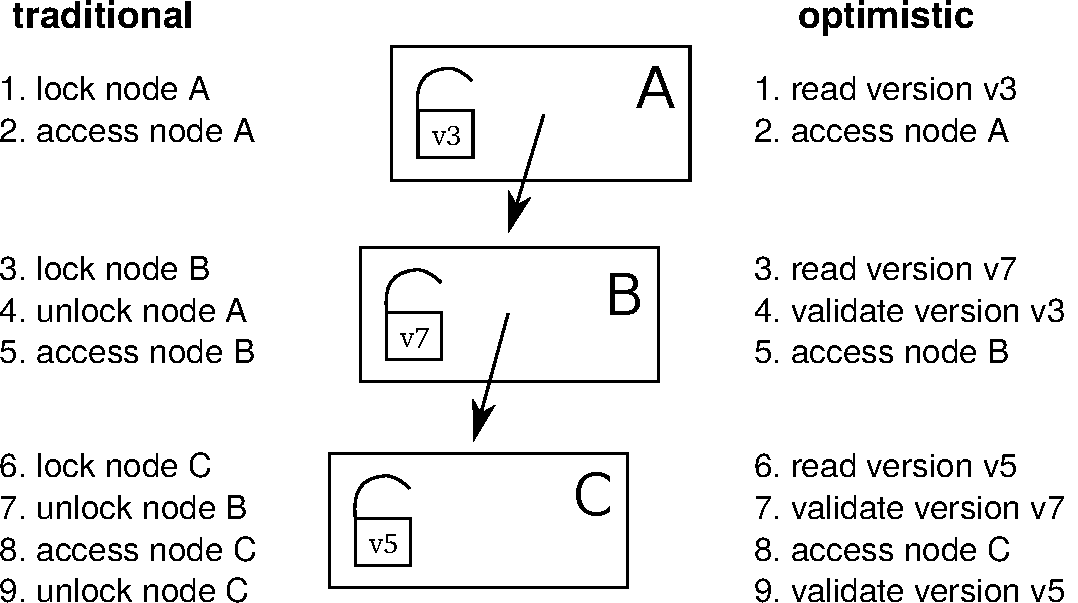
\includegraphics[width=0.65\linewidth]{olcall.pdf}
  \vspace{0.2cm}
  \caption{Comparison of a lookup operation in a 3-level tree using traditional lock coupling (left-hand side) vs.~optimistic lock coupling (right-hand side).}
  \label{fig:olc}
\end{figure}

The traditional and most common lock-based synchronization protocol for B-trees is lock coupling, which interleaves lock acquisitions while holding at most two locks at a time.
If, as we observed earlier, optimistic locks have similar semantics as traditional locks, it is natural to ask whether lock coupling can be combined with optimistic locks.
And indeed the answer is yes: One can almost mechanically translate traditional lock coupling code to optimistic lock coupling code.
This is illustrated in Figure~\ref{fig:olc}, which compares the traversal in a tree of height 3 using traditional and optimistic locks.
As the figure shows, the main difference is that locking is translated to reading the version and that unlocking becomes validation of the previously read version.
This simple change provides efficient lock-free tree traversal without the need to design a complex synchronization protocol.

It is important to emphasize the conceptual simplicity of OLC in comparison to data structures that use custom protocols like the Bw-tree~\cite{DBLP:conf/icde/LevandoskiLS13a}.
To implement lock-free access, the Bw-tree requires an indirection table, delta nodes, complex splitting and merging logic, retry logic, etc.
OLC, on the other hand, can directly be applied to B-trees mostly by adding the appropriate optimistic locking code and without modifying the node layout itself.
Therefore, OpenBw-Tree, an open source implementation of the Bw-tree, requires an order of magnitude more code than a B-tree based on OLC\footnote{Both implementations are available on GitHub: \url{https://github.com/wangziqi2016/index-microbench}}.
Given how difficult it is to develop, validate, and debug lock-free code, simplicity is obviously a major advantage.

\subsection{Correctness Aspects}

\begin{figure}
  % \centering
  %[basicstyle=\normalsize\ttfamily,showstringspaces=false,columns=fullflexible,breaklines=false,breakatwhitespace=true,numbers=none,numberstyle=\small,style=C,keepspaces=true]
\begin{lstlisting}[basicstyle=\ttfamily,language=C++,numbers=left,numberstyle=\small]
std::atomic<BTreeNode*> root;

// search for key in B+tree, returns payload in resultOut
bool lookup(Key key, Value& resultOut) {
   BTreeNode* node = root.load();
   uint64_t nodeVersion = node->readLockOrRestart();
   if (node != root.load()) // make sure the root is still the root
      restart();

   BTreeInner<Key>* parent = nullptr;
   uint64_t parentVersion = 0;

   while (node->isInner()) {
      auto inner = (BTreeInner*)node;

      // unlock parent and make current node the parent
      if (parent)
         parent->readUnlockOrRestart(parentVersion);
      parent = inner;
      parentVersion = nodeVersion;

      // search for next node
      node = inner->findChild(key);
      // validate 'inner' to ensure that 'node' pointer is valid
      inner->checkOrRestart(nodeVersion);
      // now it safe to dereference 'node' pointer (read its version)
      nodeVersion = node->readLockOrRestart();
   }

   // search in leaf and retrieve payload
   auto leaf = (BTreeLeaf*)node;
   bool success = leaf->findValue(key, resultOut);

   // unlock everything
   if (parent)
      parent->readUnlockOrRestart(parentVersion);
   node->readUnlockOrRestart(nodeVersion);

   return success;
}
\end{lstlisting}
  \vspace{0.2cm}
  \caption{B-tree lookup code using OLC. For simplicity, the restart logic is not shown.}
  \label{fig:lookup}
\end{figure}

So far, we have introduced the high-level ideas behind OLC and have stressed its similarity to traditional lock coupling.
Let us now discuss some cases where the close similarity between lock coupling and OLC breaks down.
To make this more concrete, we show the B-tree lookup code in Figure~\ref{fig:lookup}.
In the code, \texttt{readLockOrRestart} reads the lock version and \texttt{readUnlockOrRestart} validates that the read was correct.

One issue with OLC is that any pointer speculatively read from a node may point to invalid memory (if that node is modified concurrently).
Dereferencing such a pointer (e.g., to read its optimistic lock), may cause a segmentation fault or undefined behavior.
In the code shown in Figure~\ref{fig:lookup}, this problem is prevented by the extra check in line 25, which ensures that the read from the node containing the pointer was correct.
Without this additional validation, the code would in line 27 dereference the pointer speculatively read in line 23.
Note that the implementation of \texttt{checkOrRestart} is actually identical to \texttt{readUnlockOrRestart}.
We chose to give it a different name to highlight the fact that this extra check would not be necessary with read/write locks.

Another potential issue with optimistic locks is code that does not terminate.
Code that speculatively accesses a node, like an intra-node binary search, should be written in a way such that it always terminates---even in the presence of concurrent writes.
Otherwise, the validation code that detects the concurrent write will never run.
The binary search of a B-tree, for example, needs to be written in such a way that each comparison makes progress.
For some data structures that do not require loops in the traversal code (like ART) termination is trivially true.

\subsection{Implementation Details}

% implementation, efficiency
To implement an optimistic lock, one can combine the lock and the version counter into a single 64-bit\footnote{Even after subtracting one bit for the lock status, a back-of-the-envelope calculation can show that 63 bits are large enough to never overflow in practice.} word~\cite{artsync}.
A typical read operation will therefore merely consist of reading this version counter atomically.
In C++11 this can be implemented using the \texttt{std::atomic} type.

On x86, atomic reads are cheap because of x86's strong memory order guarantees.
No memory fences are required for sequentially-consistent loads, which are translated (by both GCC and clang) into standard \texttt{MOV} instructions.
Hence, the only effect of \texttt{std::atomic} for loads is preventing instruction re-ordering.
This makes version access and validation cheap.
Acquiring and releasing an optimistic lock in exclusive mode has comparable cost to a traditional lock:
A fairly expensive sequentially-consistent store is needed for acquiring a lock, while a standard \texttt{MOV} suffices for releasing it.
A simple sinlock-based implementation of optimistic locks can be found in the appendix of an earlier paper~\cite{artsync}.

OLC code must be able to handle restarts since validation or lock upgrade can fail due to concurrent writers.
Restarts can easily be implemented by wrapping the data structure operation in a loop (for simplicity not shown in Figure~\ref{fig:lookup}).
Such a loop also enables limiting the number of optimistic retry operations and falling back to pessimistic locking in cases of very heavy contention.
The ability to fall back to traditional locking is a major advantage of OLC in terms of robustness over lock-free approaches, which do not have this option.

In addition to the optimistic shared mode and the exclusive mode, optimistic locks also support a ``shared pessimistic'' mode, which physically acquires the lock in shared mode (allowing multiple concurrent readers but no writers).
This mode is useful for table (or range) scans that touch many tuples on a leaf page (which would otherwise easily abort).
Finally, let us mention that large range scans and table scans, should be broken up into several per-node traversals as is done in the LeanStore~\cite{leanstore} system.

Like all lock-free data structures, but unlike traditional locking and Hardware Transactional Memory~\cite{DBLP:conf/hpca/KarnagelDRLLSL14,DBLP:journals/pvldb/MakreshanskiLS15,htmtkde}, OLC requires care when deleting (and reusing) nodes.
The reason is that a deleting thread can never be sure that a node can be reclaimed because other threads might still be optimistically reading from that node.
Therefore, standard solutions like epoch-based reclamation~\cite{DBLP:conf/sosp/TuZKLM13}, hazard pointers~\cite{DBLP:journals/tpds/Michael04}, or optimized hazard pointers~\cite{DBLP:conf/spaa/BalmauGHZ16} need to be used.
These memory reclamation techniques are, however, largely orthogonal to the synchronization protocol itself.

%-lock-free is not a strong guarantee

\newpage
\section{Evaluation}\label{sec:evaluation}

Let us now experimentally evaluate the overhead and scalability of OLC.
For the experiments, we use an in-memory B+tree implemented in C++11 using templates, which is configured to use nodes of 4096 bytes, random 8 byte keys, and 8 byte payloads.
Based on this B-tree, we compare the following synchronization approaches:
\begin{itemize}
\item an OLC implementation\footnote{An almost identical OLC implementation is available on github: \url{https://github.com/wangziqi2016/index-microbench/tree/master/BTreeOLC}}
\item a variant based on traditional lock coupling and read/write locks
\item the unsynchronized B-tree, which obviously is only correct for read-only workloads but allows measuring the overhead of synchronization
\end{itemize}
Note that earlier work has compared the OLC implementation with a Bw-tree implementation~\cite{buzzword} and other state-of-the-art in-memory index structures.

We use a Haswell EP system with an Intel Xeon E5-2687W v3 CPU, which has 10 cores (20 ``Hyper-Threads'') and 25~MB of L3 cache.
The system is running Ubuntu 18.10 and we use GCC 8.2.0 to compile our code.
The CPU counters are obtained using the Linux perf API\footnote{We use the following convenience wrapper: \url{https://github.com/viktorleis/perfevent}}.

\begin{table}
  \caption{Performance and CPU counters for lookup and insert operations in a B-tree with 100M keys. We perform 100M operations and normalize the CPU counters by that number.}
  \label{tab:overhead}
  \centering
  \begin{tabular}{lrrrrrrr}\toprule
                    &         &        &        & instruc-  & L1     & L3     & branch \\
                    & threads & M op/s & cycles & tions & misses & misses & misses \\\midrule
lookup (no sync.)   & 1       & 1.72   & 2028   & 283     & 39.1   & 14.9   & 16.1   \\
lookup (OLC)        & 1       & 1.65   & 2107   & 370     & 43.9   & 15.1   & 16.7   \\
lookup (lock coup.) & 1       & 1.72   & 2078   & 365     & 42.3   & 16.9   & 15.7   \\\midrule
insert (no sync.)   & 1       & 1.51   & 2286   & 530     & 59.8   & 31.1   & 17.3   \\
insert (OLC)        & 1       & 1.50   & 2303   & 629     & 61.2   & 31.1   & 16.5   \\
insert (lock coup.) & 1       & 1.41   & 2473   & 644     & 61.0   & 31.0   & 17.2   \\\midrule
lookup (no sync.)   & 10      & 15.48  & 2058   & 283     & 38.6   & 15.5   & 16.0   \\
lookup (OLC)        & 10      & 14.60  & 2187   & 370     & 43.8   & 15.8   & 16.8   \\
lookup (lock coup.) & 10      & 5.71   & 5591   & 379     & 54.2   & 17.0   & 14.8   \\\midrule
insert (no sync.)   & 10      & -      & -      & -       & -      & -      & -      \\
insert (OLC)        & 10      & 10.46  & 2940   & 656     & 62.0   & 32.5   & 16.8   \\
insert (lock coup.) & 10      & 7.55   & 4161   & 667     & 75.0   & 28.6   & 16.2   \\
    \bottomrule
\end{tabular}
\end{table}

Table~\ref{tab:overhead} compares the performance and CPU counters for lookup and insert operations in a B-tree with 100M keys.
With {\em single-threaded} execution, we observe that all three approaches have very similar performance.
Adding traditional or optimistic locks to unsynchronized B-tree code results in up to 30\% of additional instructions without affecting single-threaded performance much.

\begin{figure}
  \centering
  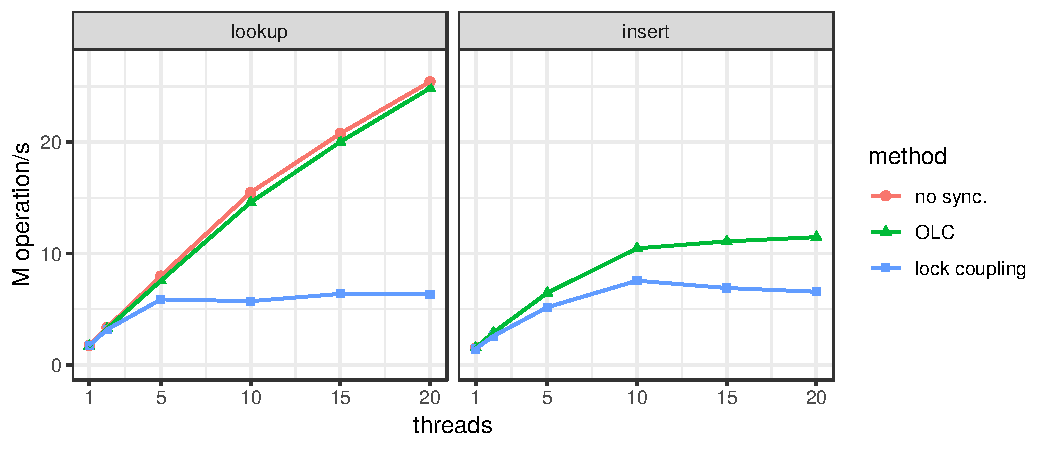
\includegraphics[width=\linewidth]{scale.pdf}
  \vspace{0.2cm}
  \caption{Scalability on 10-core system for B-tree operations (100M values).}
  \label{fig:scale}
\end{figure}

As Figure~\ref{fig:scale} shows, the results change dramatically once we use multiple threads.
For lookup, the scalability of OLC is near-linear up to 20 threads, even though the system has only 10 ``real cores''.
The OLC scalability for insert is also respectable (though not quite as linear because multi-threaded insertion approaches the memory bandwidth of our processor).
The figure also shows that the results of traditional lock coupling with read/write locks are significantly worse than OLC.
With 20 threads, lookup with OLC is 3.9$\times$ faster than traditional lock coupling.

\section{Summary}\label{sec:conc}

Optimistic Lock Coupling (OLC) is an effective synchronization method that combines the simplicity of traditional lock coupling with the superior scalability of lock-free approaches.
OLC is widely applicable and has already been successfully used to synchronize several data structures, including B-trees, binary search trees, and different trie variants.
These features make it highly attractive for modern database systems as well as performance-critical systems software in general.

\begin{thebibliography}{10}

\bibitem{DBLP:conf/spaa/BalmauGHZ16}
O.~Balmau, R.~Guerraoui, M.~Herlihy, and I.~Zablotchi.
\newblock Fast and robust memory reclamation for concurrent data structures.
\newblock In {\em SPAA}, 2016.

\bibitem{DBLP:journals/acta/BayerS77}
R.~Bayer and M.~Schkolnick.
\newblock Concurrency of operations on {B}-trees.
\newblock {\em Acta Informatica}, 9, 1977.

\bibitem{hot}
R.~Binna, E.~Zangerle, M.~Pichl, G.~Specht, and V.~Leis.
\newblock {HOT}: A height optimized trie index for main-memory database
  systems.
\newblock In {\em SIGMOD}, 2018.

\bibitem{DBLP:conf/ppopp/BronsonCCO10}
N.~G. Bronson, J.~Casper, H.~Chafi, and K.~Olukotun.
\newblock A practical concurrent binary search tree.
\newblock In {\em PPOPP}, 2010.

\bibitem{DBLP:conf/vldb/ChaHKK01}
S.~K. Cha, S.~Hwang, K.~Kim, and K.~Kwon.
\newblock Cache-conscious concurrency control of main-memory indexes on
  shared-memory multiprocessor systems.
\newblock In {\em VLDB}, 2001.

\bibitem{intel}
I.~Cutress.
\newblock {Intel} goes for 48-cores: {Cascade-AP} with multi-chip package
  coming soon.
\newblock
  \url{https://www.anandtech.com/show/13535/intel-goes-for-48cores-cascade-ap},
  2018 (accessed January, 2019).

\bibitem{DBLP:conf/cidr/FaleiroA17}
J.~M. Faleiro and D.~J. Abadi.
\newblock Latch-free synchronization in database systems: Silver bullet or
  fool's gold?
\newblock In {\em CIDR}, 2017.

\bibitem{DBLP:journals/ftdb/Graefe11}
G.~Graefe.
\newblock Modern {B}-tree techniques.
\newblock {\em Foundations and Trends in Databases}, 3(4), 2011.

\bibitem{DBLP:conf/hpca/KarnagelDRLLSL14}
T.~Karnagel, R.~Dementiev, R.~Rajwar, K.~Lai, T.~Legler, B.~Schlegel, and
  W.~Lehner.
\newblock Improving in-memory database index performance with
  {Intel}\({}^{\mbox{{\textregistered}}}\) transactional synchronization
  extensions.
\newblock In {\em HPCA}, 2014.

\bibitem{DBLP:journals/tods/LehmanY81}
P.~L. Lehman and S.~B. Yao.
\newblock Efficient locking for concurrent operations on {B}-trees.
\newblock {\em {ACM} Trans. Database Syst.}, 6(4), 1981.

\bibitem{leanstore}
V.~Leis, M.~Haubenschild, A.~Kemper, and T.~Neumann.
\newblock Leanstore: In-memory data management beyond main memory.
\newblock In {\em ICDE}, 2018.

\bibitem{art}
V.~Leis, A.~Kemper, and T.~Neumann.
\newblock The adaptive radix tree: {ARTful} indexing for main-memory databases.
\newblock In {\em ICDE}, 2013.

\bibitem{htmtkde}
V.~Leis, A.~Kemper, and T.~Neumann.
\newblock Scaling {HTM}-supported database transactions to many cores.
\newblock {\em {IEEE} Trans. Knowl. Data Eng.}, 28(2), 2016.

\bibitem{artsync}
V.~Leis, F.~Scheibner, A.~Kemper, and T.~Neumann.
\newblock The {ART} of practical synchronization.
\newblock In {\em DaMoN}, 2016.

\bibitem{DBLP:conf/icde/LevandoskiLS13a}
J.~J. Levandoski, D.~B. Lomet, and S.~Sengupta.
\newblock The {Bw}-tree: A {B}-tree for new hardware platforms.
\newblock In {\em ICDE}, 2013.

\bibitem{DBLP:journals/pvldb/MakreshanskiLS15}
D.~Makreshanski, J.~J. Levandoski, and R.~Stutsman.
\newblock To lock, swap, or elide: On the interplay of hardware transactional
  memory and lock-free indexing.
\newblock {\em {PVLDB}}, 8(11), 2015.

\bibitem{DBLP:dblp_conf/eurosys/MaoKM12}
Y.~Mao, E.~Kohler, and R.~T. Morris.
\newblock Cache craftiness for fast multicore key-value storage.
\newblock In {\em EuroSys}, 2012.

\bibitem{DBLP:journals/tpds/Michael04}
M.~M. Michael.
\newblock Hazard pointers: Safe memory reclamation for lock-free objects.
\newblock {\em {IEEE} Trans. Parallel Distrib. Syst.}, 15(6), 2004.

\bibitem{DBLP:journals/jacm/ShalevS06}
O.~Shalev and N.~Shavit.
\newblock Split-ordered lists: Lock-free extensible hash tables.
\newblock {\em J. {ACM}}, 53(3), 2006.

\bibitem{amd}
A.~Shilov.
\newblock {AMD} previews {EPYC} ‘{Rome}’ processor: Up to 64 {Zen} 2 cores.
\newblock
  \url{https://www.anandtech.com/show/13561/amd-previews-epyc-rome-processor-up-to-64-zen-2-cores},
  2018 (accessed January, 2019).

\bibitem{DBLP:conf/sosp/TuZKLM13}
S.~Tu, W.~Zheng, E.~Kohler, B.~Liskov, and S.~Madden.
\newblock Speedy transactions in multicore in-memory databases.
\newblock In {\em SOSP}, 2013.

\bibitem{buzzword}
Z.~Wang, A.~Pavlo, H.~Lim, V.~Leis, H.~Zhang, M.~Kaminsky, and D.~Andersen.
\newblock Building a {Bw}-tree takes more than just buzz words.
\newblock In {\em SIGMOD}, 2018.

\end{thebibliography}


%\bibliographystyle{abbrv}
%\bibliography{main}

\end{document}

\end{article}
\begin{article}
{Recent Approaches and Trends in Approximate Nearest Neighbor Search, with Remarks on Benchmarking}
{Martin Aum\"{u}ller, Matteo Ceccarello}
\documentclass[11pt]{article} 
\usepackage{deauthor}
\usepackage{enumitem}
\usepackage{algorithmic}
\usepackage{algorithm}
\usepackage{xcolor}
\usepackage{xspace}
\usepackage{graphicx}
\usepackage{footnote}
\usepackage{hyperref}
\usepackage{multirow}
\usepackage{subfig}
\usepackage{enumitem}
\usepackage{comment}
\usepackage{amsmath}
\usepackage{amssymb}

%\usepackage[textsize=tiny]{todonotes}
\newcommand{\matodo}[1]{\todo[inline, color=green!30]{{Martin: #1}}}
\newcommand{\mctodo}[1]{\todo[inline, color=blue!30]{{Matteo: #1}}}

\begin{document}
\title{Recent Approaches and Trends in Approximate Nearest Neighbor
	Search, with Remarks on Benchmarking} \date{}

\author{Martin Aum\"uller$^\dagger$, Matteo Ceccarello$^*$\\ $^\dagger$IT
	University of Copenhagen, maau@itu.dk \\ *University of Padova,
	matteo.ceccarello@unipd.it }



\maketitle \renewcommand\thesection{\arabic{section}}
\setcounter{section}{0} \setcounter{figure}{0} \setcounter{table}{0}

\begin{abstract}

	Nearest neighbor search is a computational primitive whose efficiency is
	paramount to many applications. As such, the literature recently blossomed
	with many works focusing on improving its effectiveness in an approximate setting.
	In this overview paper, we
	review recent advances of the state of the art and discuss some trends.
	%
	Given the practical relevance of the problem, new approaches need to be
	thoroughly benchmarked. We therefore review some recent benchmarking efforts and
	provide advice on the benchmarking pipeline.
\end{abstract}

\section{Introduction}\label{matteo_sec:introduction}

Nearest neighbor search is a key component in many computer science applications.
For example, using CLIP embeddings~\cite{DBLP:conf/icml/RadfordKHRGASAM21} both images and text can be mapped to dense vectors in a vector space; retrieving images that match a text description then boils down to embedding the text into a query vector and searching for images whose vectors are closest to the query vector under some distance measure.
Using nearest neighbor search, large language models (LLMs) can also be augmented with knowledge that was not present in the training data~\cite{DBLP:conf/iclr/KhandelwalLJZL20}.
Unfortunately, \emph{exact} nearest neighbor search in high-dimensional data---such as the dense vectors generated by deep learning-based embedding pipelines---is a notoriously difficult problem that usually requires \emph{scanning} through the whole dataset.
This excludes the possibility of scalable approaches for billion-scale datasets that are common in today's applications.

To enable scalable nearest neighbor search, the research focus turned to \emph{approximate nearest neighbor search} (ANN).
In empirical settings, this usually means that an implementation does not provide a guarantee on the quality of the returned vectors.
Instead, the user provides---based on knowledge of the data distribution and the query workloads---parameters that are used to build and to search the index data structure, respectively.
Given a query point and some search parameters, the index is used to generate a candidate set for the query.
The closest vectors among these candidates are returned as the (presumably) nearest neighbors for a given query.
The smaller the candidate set, the faster the search, but also the lower the result accuracy.
Section~\ref{matteo_sec:overview} gives an overview over general approaches to approximate nearest neighbor search.

ANN-benchmarks~\cite{DBLP:journals/is/AumullerBF20} presents the state-of-the-art benchmark on million-scale approximate nearest neighbor search implementations.
In the benchmarking run published in April 2023, more than 30 implementations were tested on a collection of datasets. Each implementation was run on a single thread.
The results for a single dataset are depicted in Figure~\ref{matteo_fig:glove}.
On a high level, many implementations achieve a throughput of more than 1,000 queries per second at an average recall of at least 90\%.
In particular, many implementations still perform well in the setting of average recall at least 99\%.
As a baseline, a bruteforce solution using BLAS achieved a throughput of 16 queries per second.
Most of the approaches that perform best implement a graph-based approach with the notable exception of Google's ScaNN~\cite{DBLP:conf/icml/GuoSLGSCK20} and Meta's FAISS~\cite{DBLP:journals/tbd/JohnsonDJ21} which both implement a clustering-based approach as their main data structure.
Please see the project website for more details on the used implementations.
We review benchmarking efforts and pitfalls in Section~\ref{matteo_sec:benchmarking}.

\begin{figure}[t!]
	\includegraphics*[width=\textwidth]{submissions/Matteo2023/figures/glove-100-angular.png}
	\caption{April 2023 run of ANN-benchmarks~\cite{DBLP:journals/is/AumullerBF20} (\url{http://ann-benchmarks.com}) on 100-dimensional vectors from GloVe embeddings~\cite{DBLP:conf/emnlp/PenningtonSM14} on a twitter corpus.
		The $x$-axis represents the average fraction of true 10-nearest neighbors returned (on a logarithmic scale); the $y$-axis provides the queries per second achieved, on a logarithmic scale.
		Both index building and searching is conducted on a single thread.
		Reported points represent the Pareto-frontier over a grid search on the parameter space.
		Interactive visualisations are available on the project website.
		Benchmarking run carried out by E. Bernhardsson.}
	\label{matteo_fig:glove}
\end{figure}

This overview paper focuses on approaches that are not covered by the current benchmarking efforts.
While theoretical breakthroughs have been achieved over the last years, for example by Andoni et al.~\cite{DBLP:conf/soda/AndoniNRW21}, our focus lies on approaches that are supported by efficient implementations targeted to solve nearest neighbor search on real-world datasets.
Section~\ref{matteo_sec:new:approaches} is dedicated to this recent work.
Finally, we close the overview by identifying recent trends and promising directions for future work in Section~\ref{matteo_sec:trends}.

\subsection{Problem setup}

Formally, the task in $k$-nearest neighbor search is defined as follows.
Let $(\mathcal{X},
	\textrm{dist})$ be a metric space, and let $k \geq 1$ be an integer. Given
a dataset $S \subseteq \mathcal{X}$ of $n$ data points $(p_1, \ldots, p_n) \in \mathcal{X}^n$, the task is to build an index data
structure that supports the following queries: Given a query point $q \in
	\mathcal{X}$, return a sequence $\mathcal{I}_q = (i_1, \ldots, i_k)$ of unique indices of
data points in $S$ such that $p_{i_1}, \ldots, p_{i_k}$ minimize the
distance to $q$.

For simplicity, we will focus on the case that $\mathcal{X} = \mathbb{R}^d$, i.e., we consider $d$-dimensional real-valued vectors.
Classical distance metrics are $L_p$ norms, in particular for $p = 2$ (Euclidean distance), and inner product dissimilarity, associated with the task commonly known as maximum inner product search.
Other interesting cases are length-$d$ bitstrings $\mathcal{X} = \{0,1\}^d$ under Hamming distance and collections of sets $\mathcal{X} = \mathcal{P}(U)$ under Jaccard similarity over a finite universe $U$ with $\mathcal{P}(U)$ being the power set of $U$.


In the case that distances are unique, we can identify by $\mathcal{I}_q^\ast$ the set of indices of the true $k$-nearest neighbors of a query point $q$.
As a quality measure, we consider the \emph{recall} $|\mathcal{I}_q \cap \mathcal{I}^\ast_q|/k$. We call a method \emph{exact} if it guarantees a recall of 1, and we call it \emph{approximate} otherwise.
In the context of approximate methods, papers often report on the \emph{average recall} over a set $Q$ of queries.
If distances are not unique, distance-based recall variants are available~\cite{DBLP:journals/is/AumullerBF20}.

\section{A general overview over high-dimensional indexing}
\label{matteo_sec:overview}

There exists a plethora of different approaches for solving nearest
neighbor search. The most successful approaches can be categorized
into \textit{clustering-based}, \textit{graph-based},
\textit{hashing-based}, and \textit{tree-based} approaches.
For the notable exception of graph-based approaches, nearest neighbor search is usually solved by partitioning the space $\mathbb{R}^d$ into $M$ disjoint parts $R_1, \ldots, R_M$ such that $\bigcup_{1 \leq i \leq M} R_i = \mathbb{R}^d$.

\subsection{Indexing techniques for high-dimensional data}

We provide a
short overview of approaches and highlight a well-established method from each category.
Each implementation comes with certain parameter choices used during the indexing phase (building the ANN data structure) and the querying phase (searching for the approximate nearest neighbors).
To ease the explanation and make an attempt of unifying the landscape, we provide explanations that focus on a single build parameter $M$ and a single search parameter $\ell$.

\paragraph{Clustering-based approaches
	(IVF~\cite{DBLP:journals/tbd/JohnsonDJ21}).} Given a dataset $S\subseteq
	\mathbb{R}^d$ and two parameters $M$ and $\ell$, run a clustering algorithm
such as $M$-means to find $M$ centroids. By associating each point with its
closest centroid, the space is partitioned into $M$ parts. The data
structure that stores the centroids and the associated lists is referred to
as an inverted file index (IVF). To find nearest neighbors to a query $q
	\in \mathbb{R}^d$, inspect the points associated to the $\ell$ closest
centroids of $q$. Since this itself is a nearest neighbor search task, for large $M$ an index over the centroids is employed.
Clustering-based approaches usually provide very compelling index size since each point is stored only once with its associated centroid.
The build time of a clustering-based approach is dominated by clustering the data points, which is often done on a sample.
The final assignment carries out $O(nM)$ distance computations to centroids if the assignment is exact; as before, this can be sped up by indexing the centroids.

\paragraph{Graph-based approaches
	(HNSW~\cite{DBLP:journals/pami/MalkovY20}).} Given a dataset $S \subseteq
	\mathbb{R}^d$ and parameters $M, \ell$, the goal is to build a graph $G =
	(V, E)$, where each point is represented by a vertex and edges exist
between a point and a ``diverse'' set of at most $M$ points. Let us
assume that such a graph $G$ is given. To find the nearest neighbors of a
query point $q$, HNSW uses a hierarchy of graphs to find a good entry point
into the bottom-layer graph that indexes all points. Given such a start
point, carry out a greedy hill climbing. In each round, consider the
currently closest point to the query not considered before. Inspect the
neighborhood and compute the distances to the query point. After each
round, trim the list of current closest points (inspected and
non-inspected) to $\ell$, which is usually called the beam width. Terminate
if all $\ell$ points have been considered. (Note that this is not a bound
on the number of distance computations, since considered points might be
trimmed off.) To build the graph, order all the points and insert them
one-by-one using the search algorithm¸ often with a smaller $\ell'$ than
used for the queries. From the points inspected in this search, a pruned
set of $M$ points is chosen as neighbors of the inserted point. Additionally, pruning
might be necessary for its neighbors if their degree bound $M$ is not met.
Graph-based indexes usually provide compelling index sizes when $M$ is small (the number of edges can be as large as $Mn$).
The index build time is usually rather high for graph-based approaches, since individual searches are carried out for each data point.


\paragraph{Hashing-based approaches
	(FALCONN~\cite{DBLP:conf/nips/AndoniILRS15})} FALCONN is an approach based
on locality-sensitive hashing optimized for inner product similarity on
unit length vectors.
It uses crosspolytope LSH as its LSH function.
A crosspolytope LSH function is described by a rotation matrix, which is chosen at random.
The hash value of a point is the closest base vector in $\mathbb{R}^d$ when applying the random rotation to the point.
Given a set of points $S$ and two parameter $M, \ell$,
the data structure works as follows.
Choose $M$ random LSH
functions mapping data points to hash values $\mathcal{R}$, where each function is the concatenation of two to three random crosspolytope LSH functions.
Hash each data
point $M$ times with independent hash function choices, and store the point in $M$ buckets, one per hash function.
These buckets together with the collection of hash functions form the index.
Given a query point and collection of $M$ hash tables, hash the query point
using the same hash functions and consider the data points that also reside
in the bucket as candidates.
Traditionally, LSH suffers from large indexes since independent repetitions provide the ``best'' buckets in the sense that among all buckets, it is most likely to find a close points in the bucket identified by the query hash code.
However, if space is a concern, one can use a smaller $M$ value and
if less than $\ell$ points are found, check
neighboring buckets using a multiprobing approach.
The index build time of a hashing-based approach is usually dominated by hashing each data point $M$ times.
Fast evaluation tricks, such as applying the fast Hadamard transform~\cite{DBLP:conf/nips/AndoniILRS15} and pooling/tensoring approaches~\cite{DBLP:conf/sisap/Christiani19} can be employed to lower this cost.

\paragraph{Tree-based approaches
	(MRPT~\cite{DBLP:conf/bigdataconf/HyvonenPTJTWCR16}).} MRPT builds a
collection of trees based on sparse random projections. Given a set of points $S$
and two parameters $M, \ell$, the data structure works as follows. First, a
node in a tree is described by a hyperplane $a$ that splits up a point set
$S' \subseteq S$. At the root, the whole dataset is taken into
consideration, and a leaf is created as soon as the number of points at a
node is below a certain threshold. Instead of a single tree, $M$ trees are
created to boost the quality of the results. Given a query point and a
collection of $M$ trees, carry out root-to-leaf-traversals in each tree for
the query. In MRPT, a voting search is carried out by considering a
point in a leaf as a candidate if it appears in at least $\nu$ different
trees.
MRPT results in compelling index sizes for small $M$ values since each level of the tree contains a single random hyperplane, only storing the split value in a node.
The build time is dominated by finding the individual splits, which typically requires in each node and over all trees, to evaluate the projection value and select the median.
\cite{DBLP:conf/pakdd/JaasaariHR19} describe a method to automatically select hyper-parameters for this approach.


\subsection{System Architecture}

\begin{figure} \includegraphics*[width=\textwidth]{submissions/Matteo2023/figures/pipeline.png}
	\caption{Overview of the phases of a traditional ANN implementation.}
	\label{matteo_fig:pipeline}
\end{figure}

The standard system architecture for ANN search is depicted in
Figure~\ref{matteo_fig:pipeline}.
Given a dataset $S \subseteq \mathcal{X}$ and a set of build parameters $\mathcal{P}_\text{build}$, an index is built following the approaches mentioned in the previous subsection.
Both the build time and the index size is often crucial for the feasibility of an approach.
Given a query point $q \in \mathcal{X}$ and a set of query parameters $\mathcal{P}_{\text{query}}$, the index is used to \emph{generate the candidate set}.
This candidate set is usually \emph{refined} using a \emph{quantization} or \emph{sketching} technique that stores small summaries of each data point.
The goal of the refinement is to discard candidate points that are \emph{unlikely} to be among the $k$ nearest neighbors.
In a final \emph{reranking step}, exact distance computations between the refined candidates and the query point are carried out, and the indices of the $k$ points with smallest distance to the query are returned as the answer to the query.
In the case that memory resources are sparse, for example when dataset vectors do not fit into main memory, the final re-ranking step might not be carried out, which usually results in a loss in precision.


\section{Benchmarking ANN implementations}
\label{matteo_sec:benchmarking}

Assessing the performance of a new method is at the same time crucial and
challenging. The new method itself often has a lot of configurations to
explore, and the number of baselines to compare with grows by the day, with
each baseline featuring a lot of parameters. In such a scenario, benchmarking
efforts such as the ANN-benchmarks~\cite{DBLP:journals/is/AumullerBF20} mentioned in the introduction---
also used for benchmarking in billion-scale settings~\cite{DBLP:conf/nips/SimhadriWADBBCH21}---
and the Lernaean Hydra framework for data series similarity~\cite{DBLP:journals/pvldb/EchihabiZPB19}
provide a very useful stepping stone.

In particular, a benchmarking infrastructure such as ANN-benchmarks provides a
collection of baseline algorithms, along with sensible ranges of their
parameters to test. Algorithms are then evaluated according to a standardized
evaluation protocol: each approach is first set up with indexing parameters;
then it is fed the data to be queried, allowing it to build index structures;
finally several query groups are executed on the same index, with different
query parameters.

We believe that it is much easier to integrate a new method in
an existing benchmarking infrastructure, rather than implementing a custom one
for each new paper. We therefore urge the community to adopt shared benchmarking
infrastructures in order both to avoid reinventing the wheel and to make results
more easily comparable across papers.
Even if the core pipeline cannot be used, the \emph{data preprocessing} (for example, the fixed definition of query workloads) and \emph{result postprocessing} (for example, the availability of groundtruth data and evaluations scripts) can be used in isolation, ensuring reproducibility of results.

Observing the evolution of results of ANN-benchmarks throughout the last couple
of years, and the experimental evaluations of the paper reviewed in this
survey, we formulate in the following a few concrete suggestions on how to
improve benchmarking of future works.

\subsection{Reporting on multiple metrics}

\begin{figure}
	\begin{minipage}{.4\textwidth}
		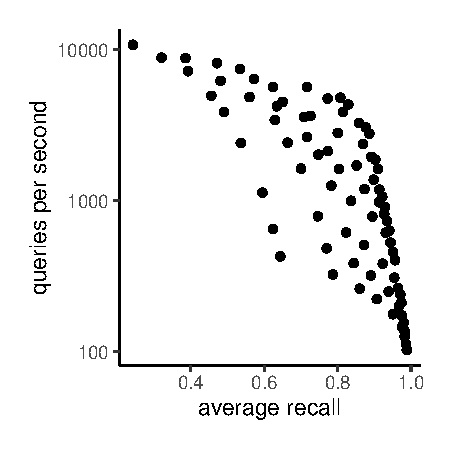
\includegraphics[width=\textwidth]{submissions/Matteo2023/figures/all_params.pdf}
		\caption{Recall/qps performance of several parameter combinations of
			HNSW on the Glove dataset.\label{matteo_fig:allparams}}
	\end{minipage}
	\hfill
	\begin{minipage}{.4\textwidth}
		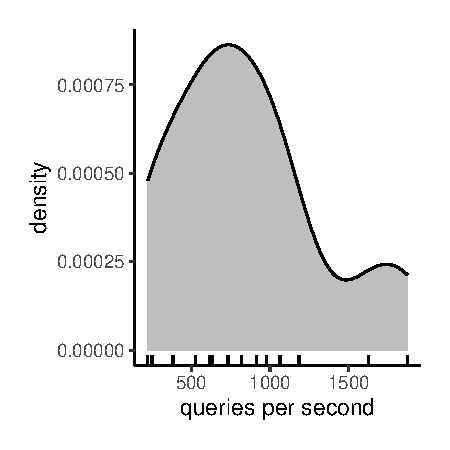
\includegraphics[width=\textwidth]{submissions/Matteo2023/figures/distribution_qps.pdf}
		\caption{Distribution of queries per second of several parameter
			combinations of HNSW achieving at least recall
			0.9.\label{matteo_fig:distribution-qps}}
	\end{minipage}
\end{figure}

Most of the times, the metrics considered for approximate
nearest neighbor queries are the query throughput and the average recall.
The query throughput---or equivalently the query time---are
however very dependent on the implementation, and are thus
measuring the performance of the implementation, rather than assessing the
merits of the underlying algorithm~\cite{DBLP:journals/kais/KriegelSZ17}.

While the actual performance of an implementation is what people are most
interested in, considering other metrics can give further insights into the
behavior of an algorithm. For instance, the number of distance
computations performed can indicate how effective an approach is at reducing
the amount of work to be performed. The interplay between the number of
distance computations and the actual running time is also of interest: a linear
scan through compressed points using product quantization may be faster than a more
sophisticated index due to better use of the cache, despite carrying out more distance
computations.
As highlighted in~\cite{DBLP:journals/corr/abs-2305-04359}, this is for example true for clustering-based
approaches compared to graph-based approaches in million-scale settings.
While the latter only carry out a fraction of distance computations, the more efficient memory layout of clustering-based approaches can make up for the additional calculations.


Furthermore, the index size and the index construction time are important
metrics to complement the execution speed.


\subsection{Selecting parameters}

Many papers evaluate the proposed method by comparing with a few state of
the art approaches, using a few configurations for each.
Some papers use just a single configuration for the baseline,
namely the default one provided by the implementation or the ones discussed in the associated publication.
This approach can however lead to misleading comparisons, in that the
performance of many approaches varies wildly in response to parameter
changes, and differently across datasets.

For instance, HNSW is a commonly used baseline to compare with, and in many
cases only a few parameter combinations are tested.
Figure~\ref{matteo_fig:allparams} reports the results---in terms of average recall
and queries per second---of answering 5\,000 queries on
\texttt{glove-100-angular}\footnote{\url{http://ann-benchmarks.com/glove-100-angular.hdf5}}
using HNSW in the implementation provided by the FAISS library~\cite{DBLP:journals/tbd/JohnsonDJ21}.
The index building parameters being used are
$M \in \{4,8,12,16,24,36,48,64,96\}$ and $efConstruction = 500$; the search parameters are varied in the range
$ef \in \{10, 20, 40, 80, 120, 200, 400, 600, 800\}$.
As one can observe, the outcomes vary wildly, both in terms of recall and
in terms of query throughput. As such, using only a single parameter
configuration as a baseline for comparison is very likely to result in
suboptimal performance for the baseline itself. In this case we consider HNSW
due to its popularity, but the same behavior can be observed with most
approaches.

Even fixing a target recall and focusing on a single configuration
achieving it does not make the performance more stable across parameter
configurations. Figure~\ref{matteo_fig:distribution-qps} shows the distribution of
the query throughput for all the aforementioned configurations that result
in an average recall between 0.9 and 0.95. As we can see, the difference
between the slowest and the fastest configurations is about two orders of
magnitude.

\subsection{Making workloads explicit}

Many papers describe which datasets are part of their experimental section and
then make a generic statement along the lines of \emph{$n$ queries are run from
	the dataset}. The reader is then left to conjecture that possibly queries are
sampled at random from the dataset. However, it has been
shown~\cite{DBLP:journals/is/AumullerC21} that the practical performance of
queries is greatly influenced by the intrinsic dimensionality of the queries
themselves. Some works already address explicitly
workloads with different
difficulties~\cite{DBLP:journals/vldb/ZoumpatianosLIP18,DBLP:journals/pvldb/EchihabiFZPB22}.

We therefore suggest to explicitly design query workloads that span a different
range of difficulties, thus allowing to assess the performance of the
approaches under test in finer detail. We provide Python code to compute
intrinsic dimensionality measures of workloads at the following public
repository: \url{https://github.com/Cecca/workloads-difficulty}.


\subsection{Dangers of reporting on averages}
\begin{figure}
	\centering
	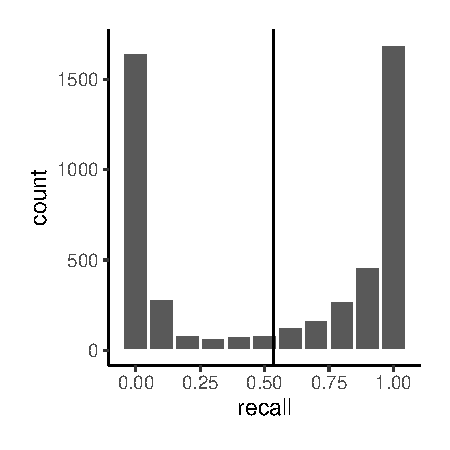
\includegraphics[width=0.4\textwidth]{submissions/Matteo2023/figures/hist_recall.pdf}
	\caption{Histogram of the recall of single queries for a configuration
		of HNSW achieving \emph{average} recall 0.55.\label{matteo_fig:hist-recall}}
\end{figure}

In the previous section we considered the average recall of 5\,000 queries
as a performance indicator.
This can be misleading at times, and hide interesting behavior.

Consider again HNSW. Figure~\ref{matteo_fig:hist-recall} reports the histogram of
the recalls of individual queries of a run attaining average recall
$\approx 0.55$\footnote{
	Using the \texttt{faiss} implementation of HNSW, with $efConstruction = 500$,
	$M = 16$ and $ef = 10$.
	Queries are the ones provided in the \texttt{glove-100-angular.hdf5} file from ANN-benchmarks.
}.
Strikingly, almost a third of the queries have recall 0, and a third
of the queries have recall 1. In this case considering the average hides
this bimodal behavior that may have important practical implications.

Therefore, we suggest to consider the distribution of the performance of
individual queries, rather than drawing conclusions based on averages alone.

\subsection{Implementation accessibility}

The possibility to access the implementation backing the findings reported in
any paper is of paramount importance for the community to verify and build upon
results.
Fortunately, in recent years the number of papers in nearest neighbor search that
make their code accessible (usually as a Git repository hosted on online services
such as GitHub or BitBucket) increased significantly.

Still, we note that code accessibility can be improved further. In some case,
the code linked to a paper fails to compile following the instructions, most
often due to differences between the environments of the code's author and the
reader. Among the many solutions to this problem, we believe the most
straightforward is to pair the code with container environments such as
Docker~\cite{DBLP:journals/sigops/Boettiger15} or
Singularity~\cite{singularity}. Doing so also makes for an easier integration
in existing benchmarking efforts, which often leverage containers in their
infrastructure~\cite{DBLP:journals/is/AumullerBF20}.

\section{New approaches to ANN search}
\label{matteo_sec:new:approaches}

Having covered general approaches to high-dimensional indexing and remarks on benchmarking efforts, we will now focus on recent work.
In the context of this overview paper, we report on approaches that appeared after the publication of the benchmarking paper~\cite{DBLP:journals/is/AumullerBF20}.

\subsection{Hashing-based Approaches}

Recent works based on hashing have focused on extending classic LSH techniques
by using new data structures, new query procedures, and by incorporating
information from the data and query distribution.

\textsc{PUFFINN}~\cite{DBLP:conf/esa/0001CPV19} is an approach whose goal
is to address approximate $k$-nearest neighbor queries while providing theoretical
guarantees on the failure probability. In order to do so, it leverages
the theoretical framework of Locality Sensitive Hashing
(LSH)~\cite{DBLP:conf/sequences/Broder97,DBLP:journals/toc/Har-PeledIM12}.
While providing theoretical
guarantees, LSH is known to have many parameters, whose setting is
crucial to achieve good performance. To overcome this issue,
\textsc{PUFFINN} adopts an \emph{adaptive} approach based on the LSH forest trie data structure~\cite{DBLP:conf/www/BawaCG05}.

\textsc{PM-LSH}~\cite{DBLP:journals/vldb/ZhengZWNLJ22}
% \footnote{Code: \url{}} 
is an approach
focusing on $L_p$ norms. Their key idea is as follows.
A dimensionality reduction using the Johnson-Lindenstrauss transform is applied to project each point into a lower-dimensional space.
The transformed points are then indexed by means of a
PM-tree~\cite{DBLP:conf/dasfaa/SkopalPS05}. Queries are then carried out
by performing several range queries on the PM-tree. While this approach
is reminiscent of the earlier SRS approach~\cite{DBLP:journals/pvldb/SunWQZL14},
there is a somehow subtle difference. Where SRS runs $k$-NN queries in
the projected space, which may suffer from the inaccuracy introduced by
the projection (i.e. the second nearest neighbor in the projected space
might not be the best candidate in the original space) PM-LSH runs a
sequence of range queries, which they demonstrate to be more accurate.

\textsc{FARGO}
% \footnote{Code:
% 	\url{https://github.com/Jacyhust/FARGO}}
~\cite{DBLP:journals/pvldb/ZhaoZYLXZJ23}
focuses on the Maximum Inner Product Search problem (MIPS). In order to
apply LSH to the MIPS problem, the paper proposes an asymmetric
transformation of data and queries so that all data points have the same
norm, while retaining the original inner products with the queries. Then
data points are indexed using LSH, and queried using a multi-probing approach.

\textsc{CEO-MIPS}~\cite{DBLP:conf/kdd/Pham21} targets the MIPS problem as well,
by performing several Gaussian random projections of the data and the queries.
By leveraging the theory of concomitants of extreme order statistics,
\textsc{CEO-MIPS} considers among all the projections of the query only the one
with maximum value. If the $i$-th projection maximizes the absolute inner product, then it considers as candidates the data points
whose $i$-th projection is large. The paper describes several variants of the
approach that reduce the space usage.

\textsc{FALCONN++}~\cite{DBLP:conf/nips/PhamL22} improves on the
Cross-Polytope-based hashing used in the FALCONN
library~\cite{DBLP:conf/nips/AndoniILRS15}.
The main insight is that
mapping a data point into a bucket based on the random vector that
maximizes the inner product (crosspolytope hashing), can also be used as an estimator of the
distance between the point and the query vector, similarly to~\cite{DBLP:conf/kdd/Pham21}.
The paper proposes a
threshold for the inner product to keep a point in a bucket, otherwise it
is filtered away. This is the first practical implementation using the
locality-sensitive filtering technique proposed by Andoni et
al.~\cite{DBLP:conf/soda/AndoniLRW17} and by
Christiani~\cite{DBLP:conf/soda/Christiani17} in the context of
approximate nearest neighbor search. We note that Rashtchian et
al.~\cite{DBLP:conf/www/RashtchianSW20} used this framework for computing similarity joins for skewed data.

\textsc{LSH-co-substring}
% \footnote{Code is available
% 	\url{https://github.com/1flei/lccs-lsh}}
~\cite{DBLP:conf/sigmod/LeiHKT20}
seeks to overcome one of the main hurdles of using LSH, that is selecting
the number of repetitions. The key idea is that, instead of performing
$L$ repetitions of the LSH scheme, each vector is associated with a
string of hash values of length $m$. Then, instead of defining buckets, a
query looks for the hash strings with the longest colliding subsequence,
allowing wraparounds at the string boundaries. The experimental analysis
shows that the approach has an edge over other LSH-based approaches in
terms of query time at a given recall, with markedly smaller index sizes.


\textsc{LSH-APG}
% \footnote{Code: \url{ https://github.com/Jacyhust/LSH-APG
% 	}}
~\cite{DBLP:journals/pvldb/ZhaoTHZZ23} aspires to blend together LSH
and graph-based approaches. In particular, LSH is used to speed up the
construction of a graph-based index. At query time, LSH is again used
to select a few entry points into the graph; these are then used to
handle the search for the best query answers. Experiments show that
LSH-APG has a larger index than graph-based methods, but such index can
indeed be constructed much faster. Furthermore, the query performance at
fixed parameters is shown to be better than other graph-based approaches.

\textsc{DB-LSH}
% \footnote{Code:
% 	\url{https://github.com/Jacyhust/DB-LSH}}
~\cite{DBLP:conf/icde/TianZZ22}
employs a \emph{dynamic bucketing} scheme, modifying the classic LSH
approach, to answer range queries. The traditional LSH approach for the
Euclidean distance requires to project points onto a random direction,
and then to bucket the projections \emph{at indexing time} to build the
hash codes. In \textsc{DB-LSH} such quantization is deferred to
\emph{query time}, so to be able to center the buckets around the query.
In particular, at index time the random projections of the dataset points
are indexed in an R*-tree. At query time, the R*-tree is used to
answer a sequence of (rectangular) range searches, that are equivalent to
dynamically bucketing the hash values around the query.

\textsc{HD-index}~\cite{DBLP:journals/pvldb/AroraSK018} answers
approximate $k$-nearest neighbor queries with the aim to use less space
than LSH. The core idea is to partition the dataset with a regular grid,
which is then traversed using a space-filling curve (such as Hilbert of
Z-order). Points are then inserted in a tree-like data structure using
their position along the space filling curve as keys. The rationale
is that points that are close in a geometric sense are also close along
the space filling curve. The experiments reported in the paper show that,
compared to baselines
the \textsc{HD-index} answers queries with a
better Mean Average Precision, in a shorter time.


\subsection{Graph-based approaches}

Graph-based approaches offer among the largest variety of known methods, see
for example the survey paper by Wang et
al.~\cite{DBLP:journals/pvldb/WangXY021}. In general, recent works have focused
on enabling the use of graph-based approaches on larger-than-memory data,
on addressing the issue of indexing time, and on designing pruning/refinement strategies for the graph building process.

\textsc{DiskANN~\cite{DBLP:conf/nips/SubramanyaDSKK19}}
targets approximate nearest neighbor search in an external memory setting,
where the size of the dataset makes it impossible to store the index and the
data entirely in memory.
Therefore, the main aim is to develop an index that minimizes the number of
disk reads per query to amortize the disk latency.
To this end, \textsc{DiskANN} refines a random
$k$-regular graph using iterated beam searches from a central graph node,
the medoid. It refines the graph in two steps with different pruning
values. In difference to HNSW, no hierarchy is employed.

\textsc{ELPIS}~\cite{DBLP:journals/pvldb/AziziEP23} tackles one of the main
issues of graph-based approaches, which is the index construction time. It
does so by first partitioning the datasets using a tree-based data
structure, and then by using HNSW to build graphs on the leaves. As such,
the graph construction is carried out in parallel on smaller subsets of the
data. This leads to a faster index construction and to a smaller index as
well.
In particular, \textsc{ELPIS} builds its tree by employing dimensionality
reduction techniques borrowed from the \emph{data series} community,
observing that a high-dimensional vector can be considered as an instance of
a data series.

Dobson et al.~\cite{DBLP:journals/corr/abs-2305-04359} give a detailed account on scaling graph-based nearest neighbor search implementations to billion-scale datasets.
In particular, they describe parallelization techniques to deal with the potential data dependencies that can occur during the parallel insertion of points.


\subsection{Clustering-based approaches}

\textsc{\textsc{SCANN}~\cite{DBLP:conf/icml/GuoSLGSCK20}} extends the
standard inverted file index based on (hierarchical) $k$-means
clustering, designed for inner product spaces. Their motivation is that
$\ell_2$-based $k$-means clustering may favor centroids that do not
preserve the ordering under inner product similarity. To mitigate this
issue, they propose an anisotropic quantization technique which is more
accurate for inner product similarity. A significant ingredient to
SCANN's performance is a very efficient product quantization
implementation based on SIMD instructions as described by Andre et
al.~\cite{DBLP:journals/pami/AndreKS21}.
Sun et al.~\cite{DBLP:conf/iclr/SunGK23} extend the approach with an efficient hyper-parameter selection technique.


\subsection{Learning-based approaches}

Algorithms with predictions~\cite{DBLP:conf/sigmod/KraskaBCDP18} is a
recent trend in the development of algorithms and data structures. The idea is that an
oracle, for example a machine learning model, gives predictions for data
that is stored in the data structure. An overview over progress in this
field in general is given by Mitzenmacher and
Vassilvitskii~\cite{DBLP:journals/cacm/MitzenmacherV22}.
A thorough survey of deep learning-based methods for approximate nearest neighbor search is given in~\cite{DBLP:journals/tkde/LiWZWFLW23}.

In the context of ANN search, two main research directions are (i) using a machine learning model to guide the candidate generation and (ii) using a machine learning model to set adaptive stopping criteria in a traditional data structure.
In the former, the indexing part is augmented with a machine learning model; in the latter, the search phase is augmented using such a model.

\textsc{ANN as Multilabel Classification} by Hyvönen et
al.~\cite{DBLP:conf/nips/HyvonenJR22} proposes to formulate the following
multi-label classification problem: Given $S \subseteq \mathcal{X}$ and
$x \in \mathcal{X}$, let $y_i = [p_i \text{ is a $k$-NN of $x$ in $S$}]$.
Thus, the (high-dimensional) label $y = (y_1, \ldots, y_n)$ represents
the set of $k$ nearest neighbors of $x$. Given these pairs $\{(x^{(i)},
	y^{(i)})\}_{1 \leq i \leq n}$, we can train a classifier for this
multi-label classification problem. Applied to space partitioning nearest
neighbor search algorithms, such as trees, LSH, or clustering-based
variants, the authors show that the pre-dominant approach that collects the
points that fall into the same part of the partition (i.e., a leaf or a
bucket) is not the \emph{natural classifier} for the multi-label
classification problem. Instead, one should use a majority vote based on
groundtruth labels $y$ of these points to decide on the candidates to
check.

\textsc{NeuralLSH}~\cite{DBLP:conf/iclr/DongIRW20} proposes to build the
$k$-NN graph on the dataset $S$, and find a balanced partition of this
graph into $m$ disjoint parts. These $m$ parts form the $m$ buckets of
the data structure. The label of a point $x$ is an $m$-bit string, where
the $i$-th bit is set if $x$ has a $k$-NN in part $i$ of the graph. The labeling
is learned by means of a neural network, and the search is guided by
predicting bucket probabilities using the neural network, and checking
all buckets in sorted order, thresholding at a certain value.

\textsc{BLISS}~\cite{DBLP:conf/kdd/GuptaMSS22} applies iterative
repartitioning by \emph{learning the bucket assignment} and
\emph{redistributing points} according to the learned assignments, in rounds. More
precisely, data points are split up at random into $B$ groups/buckets.
The label of a data point $x$ is a length-$B$ bit string; label $i \in
	\{1, \ldots, B\}$ is set if the nearest neighbor of $x$ is in group $i$.
After learning the assignment, a prediction step is carried out for each
data point, the top-$K$ buckets with the highest probability are
retrieved, and the data point is moved to the least loaded bucket among
these top-$K$. The process is repeated $R$ times independently.
Experimentally, a small value of $R$ is sufficient, and $B$ is set to
roughly $\sqrt{n}$.


\textsc{Learning to Hash, Robustly}~\cite{DBLP:conf/icml/AndoniB22} proposes a
learned LSH function for binary data under Hamming distance. In particular,
rather than sampling bit-coordinates uniformly at random as in the standard LSH
scheme, the paper describes a method to optimize the probability distribution
over coordinates, for the given dataset. In contrast to the approaches
mentioned above, they can guarantee worst-case running time comparable to the
best known theoretical approaches, while being able to adapt to the difficulty
of a query dynamically.

Li et al.~\cite{DBLP:conf/sigmod/LiZAH20} note that most approaches using
indexes to reduce the number of candidates to evaluate do not adapt to the
\emph{difficulty} of a query, i.e., use the same stopping condition for all
queries. The consequence is that to achieve a good recall a conservative
stopping condition needs to be used, thus hurting the performance of easier
queries. Therefore, they develop a prediction pipeline based on gradient
boosting decision trees, allowing the implementation of an adaptive stopping
condition. Such an adaptive stopping condition is then implemented in the IVF and
HNSW indexes, with experiments showing a general reduction in latency.


Continuing along the line of the previous paper, Zheng et
al.~\cite{DBLP:conf/icde/ZhengYHYLX0J23} focus on IVF indexes, with the aim of
setting the number of cells to probe on a per query basis. To this end, they
first modify the way data vectors are clustered, so to ensure that each cluster
has a balanced number of entries. Then they use autoencoders, trained offline
on sample queries, to estimate the number of cells to probe for a query.

\subsection{Refining Candidates}

In the context of nearest neighbor search, an important ingredient of the system pipeline is the refinement of a set of candidates.
To this end, one wants to compress vectors in a way such that points \emph{likely to not be part} of the $k$ nearest neighbors are to be excluded without incurring an exact distance computation.
A general overview of the techniques is given by Pagh in~\cite{DBLP:reference/bdt/Pagh19}.
The main technique used is Product Quantization as introduced by Jegou et al.~\cite{DBLP:journals/pami/JegouDS11}.
An overview over this technique and its variants is given by Matsui et al.~\cite{matsui2018survey}.

\textsc{FINGER}~\cite{DBLP:conf/www/ChenCJYDH23} aims at improving the speed
at which nearest neighbor graphs are traversed. The key observation is that
during traversals most of the distances do not need to be computed exactly.
Therefore, the paper proposes an estimation method to quickly estimate distances
that can be used to improve the performance of any graph-based nearest
neighbor algorithm. To showcase the performance of the approach, the paper
integrates it in an HNSW implementation.

\textsc{ADSampling}~\cite{DBLP:journals/pacmmod/GaoL23} aims at optimizing one
of the most basic operations in nearest neighbor search: the distance
comparison operation, which given a pair of points returns whether the points'
distance is above or below a given threshold. First, the same random rotation
is applied to each point. Then, given two vectors their distance is computed by
considering the rotated dimensions one at a time, in a progressive sampling
fashion, conducting a statistical hypothesis test on whether the two vectors
are closer or farther than the threshold.

\textsc{LVQ}~\cite{AuguerrebereBSHT23} describes a locally-adaptive vector quantization technique, which uses scalar quantization with individual lower and upper bounds on the coordinate values.
Employed in a graph-based index, the authors show compelling performance up to billion-scale datasets.

\section{Trends}
\label{matteo_sec:trends}

\subsection{Billion-Scale ANN search}

Scaling ANN search to billion-scale datasets has been one of the core research directions of the past years.
In particular, this is supported by the availability of diverse datasets through the NeurIPS 2021 Billion-Scale ANN challenge~\cite{DBLP:conf/nips/SimhadriWADBBCH21} and other large datasets such as Laion5B~\cite{DBLP:conf/nips/SchuhmannBVGWCC22}.
On this scale, index construction time and index size pose the most challenging part of the indexing pipeline.
Dobson et al.~\cite{DBLP:journals/corr/abs-2305-04359} provide an empirical comparison of the scaling of different approaches from million to billion scale, focusing primarily on graph-based approaches. They discuss different parallelization strategies to efficiently parallelize the index construction and the (batched) search.
They conclude that graph-based nearest neighbor search performs best on billion-scale datasets in the high recall regime.
In terms of index building times and index size, clustering- and hashing-based approaches were shown to be competitive.

\subsection{New Tasks in ANN Search}

In the following we describe extension of nearest neighbor search targeted towards real-world applications.

\paragraph{Filtered Search} When data vectors are associated with some metadata, for example for the \textsc{Yfcc-100M}~\cite{DBLP:journals/cacm/ThomeeSFENPBL16} dataset or the \textsc{Laion5B} dataset~\cite{DBLP:conf/nips/SchuhmannBVGWCC22}, a natural extension to $k$-NN search is to incorporate the metadata into the query.
Technically, each data vector is associated with a bag-of-words representation of its tags. The query vector additionally has tags $t_1,\ldots,t_T$, and the task is to find the (approximate) $k$-NN among all points in the dataset that contain the query's tags. A graph-based solution to this problem is described by Gollapudi et al.~\cite{DBLP:conf/www/GollapudiKSKBRL23-filter}.

\paragraph{Out-of-Distribution Queries}
A common scenario in modern approximate nearest neighbor search is that data and query vectors originate from different distributions, but are embedded into the same space.
For example, the Yandex \textsc{text2image} dataset~\cite{DBLP:conf/nips/SimhadriWADBBCH21} consists of image embeddings produced by the Se-ResNext-101 model described by Hu et al.~\cite{DBLP:conf/cvpr/HuSS18}, while queries are textual embeddings produced by a variant of the DSSM model by Huang et al.~\cite{DBLP:conf/cikm/HuangHGDAH13}.
As described in~\cite{DBLP:conf/nips/SimhadriWADBBCH21}, the mapping to the shared 200-dimensional real valued vectors under inner product similarity is learned via minimizing a variant of the triplet loss using clickthrough data.
A novel approach to explicitly deal with out-of-distribution queries is described in~\cite{DBLP:journals/corr/abs-2211-12850-ood}.
As pointed out in~\cite{DBLP:journals/corr/abs-2305-04359}, cluster- and LSH-based approaches are particularly affected by these changes in distribution.


\paragraph{Streaming Search}
A particular challenge in the index building process is to maintain an index over dynamic insertions and deletions.
Technically, a stream of \emph{add}, \emph{delete}, \emph{search} operations is given, where each search is supposed to return the approximate $k$-nearest neighbors of all the elements that are in the index according to the \emph{add} and \emph{delete} operations.
Simhadri~\footnote{\url{https://harsha-simhadri.org/pubs/ANNS-talk-Sep22.pptx}, (accessed on Sept 25, 2023.)} describes different applications of this setting.
For example, for web search the index may contain roughly a trillion vectors and has to handle billions of updates per day.
Searches have to be handled at a latency of at most 10 milliseconds with a throughput of 10,000-100,000 queries per second.
Naïve solutions such as placing tombstones for deleted items quickly degrade performance, as would a complete rebuild of the index in a given interval size.
Singh et al.~\cite{DBLP:journals/corr/abs-2105-09613-stream} describe a graph-based approach to handle this issue and show competitive performance to the non-stream setting, and a big improvement over previous LSH-based approaches~\cite{DBLP:journals/pvldb/SundaramTSMIMD13}.
Their system handles thousands of add/delete operations per second while maintaining high recall/throughput comparable to the non-streaming setting.
A special case of this dynamic setting is \emph{content drift}, which was studied by Baranchuk et al.~\cite{DBLP:journals/corr/abs-2308-02752-drift}.


\subsection{Conclusions}

In recent years, the field of approximate nearest
neighbor search has witnessed an exciting surge in the development of new approaches and the refinement of existing methods. Alongside the
traditional $k$-nearest neighbor setting, new tasks are emerging:
queries can incorporate different metadata such as tags, an index has to be kept over a dynamic stream of search, insert, and remove operations, or queries might arise from a different
distribution than the data points. Moreover, the scale of today's datasets has reached billions of data points, requiring unprecedented scalability while retaining
accuracy.

Given the practical relevance of the problem, it is crucial that new approaches
are benchmarked thoroughly. Given the effort needed to set up a benchmarking
infrastructure, we invite the research community to adopt and improve shared benchmarks which avoid the pitfalls that commonly affect experimental evaluations.



\paragraph{Acknowledgements:} Martin Aumüller thanks Yusuke Matsui for insightful discussions. He also thanks his collaborators
organizing and working on approximate nearest neighbor search challenges
\cite{DBLP:conf/nips/SimhadriWADBBCH21,sisap23challenge}, and the NeurIPS'23 challenge\footnote{\url{https://big-ann-benchmarks.com/}}. This research was supported by the Innovation Fund Denmark for the project DIREC
(9142-00001B).

\bibliographystyle{plainnat} 
\bibliography{submissions/Matteo2023/references}

\end{document}


\end{article}
\end{articlesection}

% put the news items below- there can be multiple news sections
% each with its own title
% news will usually have an author as well as a title,
% e.g. TCDE elections
% news articles are in the same format as letters
% typically, news articles will be stored in a directory called "news"


% \begin{newssection}{Obituary}
% \begin{news}{Obituary for Professor Gio Wiederhold}
% {Kyu-Young Whang and Marianne Winslett}{Distinguished Professor Emeritus, KAIST\\ Research Professor Emerita, UIUC\\ together with Gio’s other former students}
% \documentclass[11pt]{article} 

\usepackage{deauthor,times,graphicx}
%\usepackage{url}
\usepackage{hyperref}

\begin{document}
%Obituary for Professor Gio Wiederhold
%                                                                  December 26, 2022                                                                         
Professor Gio Wiederhold passed away in the early hours of December 26, 2022, aged 86, just 10 weeks after an unexpected diagnosis of stage 4 liver cancer. Gio died at home, surrounded by his family members who had gathered for Christmas, including his wife of 56 years, Voy Wiederhold, and his sons John and Randy.  


Gio was a great scholar, educator, and mentor. His influence on the database field is immense. As a pioneer in the database field, he wrote the influential 1977 textbook Database Design, one of the first in the field and adopted around the world. In his DARPA-supported Knowledge-Base Management Systems project in the early 1980s, Gio pioneered the concept of integrating databases and AI, a topic that is now enjoying a revival. Beginning in the 1970s, Gio also pursued the application of databases to medical informatics, another area just now entering the mainstream. In 1992, Gio introduced the notion of mediators (IEEE Computer) as a way of intelligently integrating information from large-scale heterogeneous sources such as databases, file systems, and repositories, a seminal idea for the nascent field of information integration. Gio continued to innovate after retirement from Stanford, most notably in establishing an approach for valuing software and the intellectual property of multinational firms.


Gio advised 36 PhD students at Stanford. Today, Gio’s academic descendants can be found in companies and universities all over the world, including early students Hector Garcia-Molina (the late Stanford professor), David Shaw (DE Shaw founder), Ramez Elmasri (the late textbook author and UT Arlington professor), Kyu-Young Whang (KAIST professor and Naver founder’s advisor), and Marianne Winslett (UIUC professor). Gio’s many subsequent students continue to lead the database field today. 


An influential mentor, Gio always emphasized the practical aspects of research, encouraging people to develop both theoretical and engineering approaches to solve real-world problems. This outlook stemmed from his many years of experience in computing practice before he joined the Stanford University faculty.


Gio’s service to the professional community includes serving as the third Editor-in-Chief of ACM Transactions on Databases during 1985-1995, during which time he significantly contributed to making the new journal a top one in the field. Together with five colleagues, Gio co-founded the IEEE International Conference on Data Engineering in 1984. Perhaps the first venue to use the term data engineering, the conference was unique in focusing on engineering aspects of database research; today it stands as one of the three top-tier conferences in database research. Gio also served as the conference’s program committee chair, co-chair, and general chair in its early years. During 1991-1994, Gio served as the program manager for DARPA’s Knowledge-based Systems program, which collaborated with NSF to fund innovative new research related to information integration and digital libraries — including the project that led to the creation of Google.


In recognition of his many contributions, Gio received the IEEE Technical Community on Data Engineering’s Service Award in 2016. He was also a Fellow of the ACM, the IEEE, and the American College of Medical Informatics.




The many accomplishments and contributions listed above do not capture the full extent of Gio’s impact and influence on our community, nor his diligence and persistence. As Gio’s former students, we dearly miss him for his warm heart towards his students, colleagues, and friends, and above all, his love and kindness for everyone he knew. We are deeply saddened by Gio’s unexpected death and send our sincerest condolences to his surviving family and friends.  




%-- Kyu-Young Whang, Distinguished Professor Emeritus, KAIST and Marianne Winslett, Research Professor Emerita, University of Illinois at Urbana-Champaign, together with Gio’s other former students
\end{document}

% \end{news}

% \newpage
% \end{newssection}


\begin{callsection}

%  This section will be empty for your version
%
%  Calls for papers section.  Use the callsection environment.
%  Each call for papers is contained in an call environment, where the single
%  required options to \begin{call} is the name of the conference.
% typically calls are stored in a "calls" directory
%
%\begin{call}{name of conference}
%\centerline{\includegraphics[width=\textwidth, bb= 0 0 590 760]{calls/conference-name.pdf}}
%\end{call}
%\begin{call}{ICDE 2019 Conference}
%\centerline{
\includegraphics[width=\textwidth, bb= 0 0 610 790] {../Dec-2018/calls/icde19.pdf}}
%\centerline{
\includegraphics[width=\textwidth, bb= 0 0 590 760] {calls/icde19.pdf}}
%\end{call}
\begin{call}{TCDE Membership Form}
%\centerline{\includegraphics[width=\textwidth, bb= 0 0 610 790]
%\centerline{
\includegraphics[width=\textwidth, bb= 0 0 590 760] {../Dec-2018/calls/tcde.pdf}}
\centerline{
\includegraphics[width=\textwidth, bb= 0 0 590 760] {./calls/tcde.pdf}}
\end{call}

\end{callsection}

\end{bulletin}
\end{document}
